\documentclass[twoside]{book}

% Packages required by doxygen
\usepackage{fixltx2e}
\usepackage{calc}
\usepackage{doxygen}
\usepackage[export]{adjustbox} % also loads graphicx
\usepackage{graphicx}
\usepackage[utf8]{inputenc}
\usepackage{makeidx}
\usepackage{multicol}
\usepackage{multirow}
\PassOptionsToPackage{warn}{textcomp}
\usepackage{textcomp}
\usepackage[nointegrals]{wasysym}
\usepackage[table]{xcolor}

% Font selection
\usepackage[T1]{fontenc}
\usepackage[scaled=.90]{helvet}
\usepackage{courier}
\usepackage{amssymb}
\usepackage{sectsty}
\renewcommand{\familydefault}{\sfdefault}
\allsectionsfont{%
  \fontseries{bc}\selectfont%
  \color{darkgray}%
}
\renewcommand{\DoxyLabelFont}{%
  \fontseries{bc}\selectfont%
  \color{darkgray}%
}
\newcommand{\+}{\discretionary{\mbox{\scriptsize$\hookleftarrow$}}{}{}}

% Page & text layout
\usepackage{geometry}
\geometry{%
  a4paper,%
  top=2.5cm,%
  bottom=2.5cm,%
  left=2.5cm,%
  right=2.5cm%
}
\tolerance=750
\hfuzz=15pt
\hbadness=750
\setlength{\emergencystretch}{15pt}
\setlength{\parindent}{0cm}
\setlength{\parskip}{0.2cm}
\makeatletter
\renewcommand{\paragraph}{%
  \@startsection{paragraph}{4}{0ex}{-1.0ex}{1.0ex}{%
    \normalfont\normalsize\bfseries\SS@parafont%
  }%
}
\renewcommand{\subparagraph}{%
  \@startsection{subparagraph}{5}{0ex}{-1.0ex}{1.0ex}{%
    \normalfont\normalsize\bfseries\SS@subparafont%
  }%
}
\makeatother

% Headers & footers
\usepackage{fancyhdr}
\pagestyle{fancyplain}
\fancyhead[LE]{\fancyplain{}{\bfseries\thepage}}
\fancyhead[CE]{\fancyplain{}{}}
\fancyhead[RE]{\fancyplain{}{\bfseries\leftmark}}
\fancyhead[LO]{\fancyplain{}{\bfseries\rightmark}}
\fancyhead[CO]{\fancyplain{}{}}
\fancyhead[RO]{\fancyplain{}{\bfseries\thepage}}
\fancyfoot[LE]{\fancyplain{}{}}
\fancyfoot[CE]{\fancyplain{}{}}
\fancyfoot[RE]{\fancyplain{}{\bfseries\scriptsize Generated on Wed Oct 28 2015 02\+:56\+:19 for Mol\+Sim by Doxygen }}
\fancyfoot[LO]{\fancyplain{}{\bfseries\scriptsize Generated on Wed Oct 28 2015 02\+:56\+:19 for Mol\+Sim by Doxygen }}
\fancyfoot[CO]{\fancyplain{}{}}
\fancyfoot[RO]{\fancyplain{}{}}
\renewcommand{\footrulewidth}{0.4pt}
\renewcommand{\chaptermark}[1]{%
  \markboth{#1}{}%
}
\renewcommand{\sectionmark}[1]{%
  \markright{\thesection\ #1}%
}

% Indices & bibliography
\usepackage{natbib}
\usepackage[titles]{tocloft}
\setcounter{tocdepth}{3}
\setcounter{secnumdepth}{5}
\makeindex

% Hyperlinks (required, but should be loaded last)
\usepackage{ifpdf}
\ifpdf
  \usepackage[pdftex,pagebackref=true]{hyperref}
\else
  \usepackage[ps2pdf,pagebackref=true]{hyperref}
\fi
\hypersetup{%
  colorlinks=true,%
  linkcolor=blue,%
  citecolor=blue,%
  unicode%
}

% Custom commands
\newcommand{\clearemptydoublepage}{%
  \newpage{\pagestyle{empty}\cleardoublepage}%
}


%===== C O N T E N T S =====

\begin{document}

% Titlepage & ToC
\hypersetup{pageanchor=false,
             bookmarks=true,
             bookmarksnumbered=true,
             pdfencoding=unicode
            }
\pagenumbering{roman}
\begin{titlepage}
\vspace*{7cm}
\begin{center}%
{\Large Mol\+Sim }\\
\vspace*{1cm}
{\large Generated by Doxygen 1.8.9.1}\\
\vspace*{0.5cm}
{\small Wed Oct 28 2015 02:56:19}\\
\end{center}
\end{titlepage}
\clearemptydoublepage
\tableofcontents
\clearemptydoublepage
\pagenumbering{arabic}
\hypersetup{pageanchor=true}

%--- Begin generated contents ---
\chapter{Namespace Index}
\section{Namespace List}
Here is a list of all namespaces with brief descriptions\+:\begin{DoxyCompactList}
\item\contentsline{section}{\hyperlink{namespaceoutputWriter}{output\+Writer} }{\pageref{namespaceoutputWriter}}{}
\item\contentsline{section}{\hyperlink{namespaceutils}{utils} }{\pageref{namespaceutils}}{}
\item\contentsline{section}{\hyperlink{namespacexml__schema}{xml\+\_\+schema} \\*C++ namespace for the http\+://www.w3.\+org/2001/\+X\+M\+L\+Schema schema namespace }{\pageref{namespacexml__schema}}{}
\item\contentsline{section}{\hyperlink{namespacexml__schema_1_1dom}{xml\+\_\+schema\+::dom} \\*D\+O\+M interaction }{\pageref{namespacexml__schema_1_1dom}}{}
\end{DoxyCompactList}

\chapter{Hierarchical Index}
\section{Class Hierarchy}
This inheritance list is sorted roughly, but not completely, alphabetically\+:\begin{DoxyCompactList}
\item \contentsline{section}{File\+Reader}{\pageref{classFileReader}}{}
\item list\begin{DoxyCompactList}
\item \contentsline{section}{Data\+Array\+List\+\_\+t}{\pageref{classDataArrayList__t}}{}
\begin{DoxyCompactList}
\item \contentsline{section}{Data\+Array\+\_\+t}{\pageref{classDataArray__t}}{}
\end{DoxyCompactList}
\end{DoxyCompactList}
\item \contentsline{section}{Particle}{\pageref{classParticle}}{}
\item \contentsline{section}{Particle\+Container}{\pageref{classParticleContainer}}{}
\item simple\+\_\+type\begin{DoxyCompactList}
\item \contentsline{section}{Data\+Array\+List\+\_\+t}{\pageref{classDataArrayList__t}}{}
\end{DoxyCompactList}
\item string\begin{DoxyCompactList}
\item \contentsline{section}{type}{\pageref{classtype}}{}
\end{DoxyCompactList}
\item type\begin{DoxyCompactList}
\item \contentsline{section}{Cell\+Data}{\pageref{classCellData}}{}
\item \contentsline{section}{Cells}{\pageref{classCells}}{}
\item \contentsline{section}{Piece\+Unstructured\+Grid\+\_\+t}{\pageref{classPieceUnstructuredGrid__t}}{}
\item \contentsline{section}{Point\+Data}{\pageref{classPointData}}{}
\item \contentsline{section}{Points}{\pageref{classPoints}}{}
\item \contentsline{section}{Poly\+Data\+\_\+t}{\pageref{classPolyData__t}}{}
\item \contentsline{section}{Unstructured\+Grid\+\_\+t}{\pageref{classUnstructuredGrid__t}}{}
\item \contentsline{section}{V\+T\+K\+File\+\_\+t}{\pageref{classVTKFile__t}}{}
\end{DoxyCompactList}
\item \contentsline{section}{utils\+:\+:Vector$<$ type, length $>$}{\pageref{classutils_1_1Vector}}{}
\item \contentsline{section}{utils\+:\+:Vector$<$ double, 3 $>$}{\pageref{classutils_1_1Vector}}{}
\item \contentsline{section}{output\+Writer\+:\+:V\+T\+K\+Writer}{\pageref{classoutputWriter_1_1VTKWriter}}{}
\item \contentsline{section}{output\+Writer\+:\+:X\+Y\+Z\+Writer}{\pageref{classoutputWriter_1_1XYZWriter}}{}
\end{DoxyCompactList}

\chapter{Class Index}
\section{Class List}
Here are the classes, structs, unions and interfaces with brief descriptions\+:\begin{DoxyCompactList}
\item\contentsline{section}{\hyperlink{classCellData}{Cell\+Data} \\*Class corresponding to the Cell\+Data schema type }{\pageref{classCellData}}{}
\item\contentsline{section}{\hyperlink{classCells}{Cells} \\*Class corresponding to the Cells schema type }{\pageref{classCells}}{}
\item\contentsline{section}{\hyperlink{classDataArray__t}{Data\+Array\+\_\+t} \\*Class corresponding to the Data\+Array\+\_\+t schema type }{\pageref{classDataArray__t}}{}
\item\contentsline{section}{\hyperlink{classDataArrayList__t}{Data\+Array\+List\+\_\+t} \\*List class corresponding to the Data\+Array\+List\+\_\+t schema type }{\pageref{classDataArrayList__t}}{}
\item\contentsline{section}{\hyperlink{classFileReader}{File\+Reader} }{\pageref{classFileReader}}{}
\item\contentsline{section}{\hyperlink{classParticle}{Particle} }{\pageref{classParticle}}{}
\item\contentsline{section}{\hyperlink{classParticleContainer}{Particle\+Container} }{\pageref{classParticleContainer}}{}
\item\contentsline{section}{\hyperlink{classPieceUnstructuredGrid__t}{Piece\+Unstructured\+Grid\+\_\+t} \\*Class corresponding to the Piece\+Unstructured\+Grid\+\_\+t schema type }{\pageref{classPieceUnstructuredGrid__t}}{}
\item\contentsline{section}{\hyperlink{classPointData}{Point\+Data} \\*Class corresponding to the Point\+Data schema type }{\pageref{classPointData}}{}
\item\contentsline{section}{\hyperlink{classPoints}{Points} \\*Class corresponding to the Points schema type }{\pageref{classPoints}}{}
\item\contentsline{section}{\hyperlink{classPolyData__t}{Poly\+Data\+\_\+t} \\*Class corresponding to the Poly\+Data\+\_\+t schema type }{\pageref{classPolyData__t}}{}
\item\contentsline{section}{\hyperlink{classtype}{type} \\*Enumeration class corresponding to the type schema type }{\pageref{classtype}}{}
\item\contentsline{section}{\hyperlink{classUnstructuredGrid__t}{Unstructured\+Grid\+\_\+t} \\*Class corresponding to the Unstructured\+Grid\+\_\+t schema type }{\pageref{classUnstructuredGrid__t}}{}
\item\contentsline{section}{\hyperlink{classutils_1_1Vector}{utils\+::\+Vector$<$ type, length $>$} }{\pageref{classutils_1_1Vector}}{}
\item\contentsline{section}{\hyperlink{classVTKFile__t}{V\+T\+K\+File\+\_\+t} \\*Class corresponding to the V\+T\+K\+File\+\_\+t schema type }{\pageref{classVTKFile__t}}{}
\item\contentsline{section}{\hyperlink{classoutputWriter_1_1VTKWriter}{output\+Writer\+::\+V\+T\+K\+Writer} }{\pageref{classoutputWriter_1_1VTKWriter}}{}
\item\contentsline{section}{\hyperlink{classoutputWriter_1_1XYZWriter}{output\+Writer\+::\+X\+Y\+Z\+Writer} }{\pageref{classoutputWriter_1_1XYZWriter}}{}
\end{DoxyCompactList}

\chapter{File Index}
\section{File List}
Here is a list of all files with brief descriptions\+:\begin{DoxyCompactList}
\item\contentsline{section}{src/\hyperlink{FileReader_8cpp}{File\+Reader.\+cpp} }{\pageref{FileReader_8cpp}}{}
\item\contentsline{section}{src/\hyperlink{FileReader_8h}{File\+Reader.\+h} }{\pageref{FileReader_8h}}{}
\item\contentsline{section}{src/\hyperlink{MolSim_8cpp}{Mol\+Sim.\+cpp} }{\pageref{MolSim_8cpp}}{}
\item\contentsline{section}{src/\hyperlink{Particle_8cpp}{Particle.\+cpp} }{\pageref{Particle_8cpp}}{}
\item\contentsline{section}{src/\hyperlink{Particle_8h}{Particle.\+h} }{\pageref{Particle_8h}}{}
\item\contentsline{section}{src/\hyperlink{ParticleContainer_8cpp}{Particle\+Container.\+cpp} }{\pageref{ParticleContainer_8cpp}}{}
\item\contentsline{section}{src/\hyperlink{ParticleContainer_8h}{Particle\+Container.\+h} }{\pageref{ParticleContainer_8h}}{}
\item\contentsline{section}{src/\hyperlink{Test_8cpp}{Test.\+cpp} }{\pageref{Test_8cpp}}{}
\item\contentsline{section}{src/output\+Writer/\hyperlink{vtk-unstructured_8cpp}{vtk-\/unstructured.\+cpp} }{\pageref{vtk-unstructured_8cpp}}{}
\item\contentsline{section}{src/output\+Writer/\hyperlink{vtk-unstructured_8h}{vtk-\/unstructured.\+h} \\*Generated from vtk-\/unstructured.\+xsd }{\pageref{vtk-unstructured_8h}}{}
\item\contentsline{section}{src/output\+Writer/\hyperlink{VTKWriter_8cpp}{V\+T\+K\+Writer.\+cpp} }{\pageref{VTKWriter_8cpp}}{}
\item\contentsline{section}{src/output\+Writer/\hyperlink{VTKWriter_8h}{V\+T\+K\+Writer.\+h} }{\pageref{VTKWriter_8h}}{}
\item\contentsline{section}{src/output\+Writer/\hyperlink{XYZWriter_8cpp}{X\+Y\+Z\+Writer.\+cpp} }{\pageref{XYZWriter_8cpp}}{}
\item\contentsline{section}{src/output\+Writer/\hyperlink{XYZWriter_8h}{X\+Y\+Z\+Writer.\+h} }{\pageref{XYZWriter_8h}}{}
\item\contentsline{section}{src/utils/\hyperlink{Vector_8h}{Vector.\+h} }{\pageref{Vector_8h}}{}
\end{DoxyCompactList}

\chapter{Namespace Documentation}
\hypertarget{namespaceoutputWriter}{}\section{output\+Writer Namespace Reference}
\label{namespaceoutputWriter}\index{output\+Writer@{output\+Writer}}
\subsection*{Classes}
\begin{DoxyCompactItemize}
\item 
class \hyperlink{classoutputWriter_1_1VTKWriter}{V\+T\+K\+Writer}
\item 
class \hyperlink{classoutputWriter_1_1XYZWriter}{X\+Y\+Z\+Writer}
\end{DoxyCompactItemize}

\hypertarget{namespaceutils}{}\section{utils Namespace Reference}
\label{namespaceutils}\index{utils@{utils}}
\subsection*{Classes}
\begin{DoxyCompactItemize}
\item 
class \hyperlink{classutils_1_1Vector}{Vector}
\end{DoxyCompactItemize}

\hypertarget{namespacexml__schema}{}\section{xml\+\_\+schema Namespace Reference}
\label{namespacexml__schema}\index{xml\+\_\+schema@{xml\+\_\+schema}}


C++ namespace for the http\+://www.w3.\+org/2001/\+X\+M\+L\+Schema schema namespace.  


\subsection*{Namespaces}
\begin{DoxyCompactItemize}
\item 
 \hyperlink{namespacexml__schema_1_1dom}{dom}
\begin{DoxyCompactList}\small\item\em D\+O\+M interaction. \end{DoxyCompactList}\end{DoxyCompactItemize}
\subsection*{Typedefs}
\begin{DoxyCompactItemize}
\item 
typedef \+::xsd\+::cxx\+::tree\+::type \hyperlink{namespacexml__schema_a3d277dc807f2e4ec4261dcef5c04a836}{type}
\begin{DoxyCompactList}\small\item\em C++ type corresponding to the any\+Type X\+M\+L Schema built-\/in type. \end{DoxyCompactList}\item 
typedef \+::xsd\+::cxx\+::tree\+::simple\+\_\+type$<$ \hyperlink{namespacexml__schema_a3d277dc807f2e4ec4261dcef5c04a836}{type} $>$ \hyperlink{namespacexml__schema_a44789bb4367951bcf8ae867cb983324d}{simple\+\_\+type}
\begin{DoxyCompactList}\small\item\em C++ type corresponding to the any\+Simple\+Type X\+M\+L Schema built-\/in type. \end{DoxyCompactList}\item 
typedef \+::xsd\+::cxx\+::tree\+::type \hyperlink{namespacexml__schema_a395f5179c5fc4643909d66e9ff28d8ca}{container}
\begin{DoxyCompactList}\small\item\em Alias for the any\+Type type. \end{DoxyCompactList}\item 
typedef signed char \hyperlink{namespacexml__schema_a2a462724b41fb68016d13b34f9a84b7d}{byte}
\begin{DoxyCompactList}\small\item\em C++ type corresponding to the byte X\+M\+L Schema built-\/in type. \end{DoxyCompactList}\item 
typedef unsigned char \hyperlink{namespacexml__schema_a876b68656d976c6343512f3d44fe8ca2}{unsigned\+\_\+byte}
\begin{DoxyCompactList}\small\item\em C++ type corresponding to the unsigned\+Byte X\+M\+L Schema built-\/in type. \end{DoxyCompactList}\item 
typedef short \hyperlink{namespacexml__schema_a705720c1fed1575ccdcfd21cb7ab39ab}{short\+\_\+}
\begin{DoxyCompactList}\small\item\em C++ type corresponding to the short X\+M\+L Schema built-\/in type. \end{DoxyCompactList}\item 
typedef unsigned short \hyperlink{namespacexml__schema_a7fc7b4a846c512c370346e15dfdcecaa}{unsigned\+\_\+short}
\begin{DoxyCompactList}\small\item\em C++ type corresponding to the unsigned\+Short X\+M\+L Schema built-\/in type. \end{DoxyCompactList}\item 
typedef int \hyperlink{namespacexml__schema_acfa24ac68e1a188e7f44c36f7a158bf4}{int\+\_\+}
\begin{DoxyCompactList}\small\item\em C++ type corresponding to the int X\+M\+L Schema built-\/in type. \end{DoxyCompactList}\item 
typedef unsigned int \hyperlink{namespacexml__schema_a85ca3205d8af287e149aac54535f57e7}{unsigned\+\_\+int}
\begin{DoxyCompactList}\small\item\em C++ type corresponding to the unsigned\+Int X\+M\+L Schema built-\/in type. \end{DoxyCompactList}\item 
typedef long long \hyperlink{namespacexml__schema_a1d78aacee49e26cb7a69d5aa97df1268}{long\+\_\+}
\begin{DoxyCompactList}\small\item\em C++ type corresponding to the long X\+M\+L Schema built-\/in type. \end{DoxyCompactList}\item 
typedef unsigned long long \hyperlink{namespacexml__schema_a4413fbcf4c65ffc7aaafe465d72fcb33}{unsigned\+\_\+long}
\begin{DoxyCompactList}\small\item\em C++ type corresponding to the unsigned\+Long X\+M\+L Schema built-\/in type. \end{DoxyCompactList}\item 
typedef long long \hyperlink{namespacexml__schema_aaaea7c8ce4dfbe26cc52c91c29c97b7c}{integer}
\begin{DoxyCompactList}\small\item\em C++ type corresponding to the integer X\+M\+L Schema built-\/in type. \end{DoxyCompactList}\item 
typedef long long \hyperlink{namespacexml__schema_a3de6073e510eb8edd71ddc6e0256e2f9}{non\+\_\+positive\+\_\+integer}
\begin{DoxyCompactList}\small\item\em C++ type corresponding to the non\+Positive\+Integer X\+M\+L Schema built-\/in type. \end{DoxyCompactList}\item 
typedef unsigned long long \hyperlink{namespacexml__schema_af42ef5911d65f41a0a03598b056f05aa}{non\+\_\+negative\+\_\+integer}
\begin{DoxyCompactList}\small\item\em C++ type corresponding to the non\+Negative\+Integer X\+M\+L Schema built-\/in type. \end{DoxyCompactList}\item 
typedef unsigned long long \hyperlink{namespacexml__schema_abe9d639a15a121d2868ae2f9c974ca24}{positive\+\_\+integer}
\begin{DoxyCompactList}\small\item\em C++ type corresponding to the positive\+Integer X\+M\+L Schema built-\/in type. \end{DoxyCompactList}\item 
typedef long long \hyperlink{namespacexml__schema_acf9528a84381d07f2802785c947bf441}{negative\+\_\+integer}
\begin{DoxyCompactList}\small\item\em C++ type corresponding to the negative\+Integer X\+M\+L Schema built-\/in type. \end{DoxyCompactList}\item 
typedef bool \hyperlink{namespacexml__schema_ae5ada4ec9c54b51765c3e4c0e9631bba}{boolean}
\begin{DoxyCompactList}\small\item\em C++ type corresponding to the boolean X\+M\+L Schema built-\/in type. \end{DoxyCompactList}\item 
typedef float \hyperlink{namespacexml__schema_ad7e04ab17bba0b3fdde43fb79ef6ed87}{float\+\_\+}
\begin{DoxyCompactList}\small\item\em C++ type corresponding to the float X\+M\+L Schema built-\/in type. \end{DoxyCompactList}\item 
typedef double \hyperlink{namespacexml__schema_aac2d3d3483d3a20e8d96d2e8e5b3a470}{double\+\_\+}
\begin{DoxyCompactList}\small\item\em C++ type corresponding to the double X\+M\+L Schema built-\/in type. \end{DoxyCompactList}\item 
typedef double \hyperlink{namespacexml__schema_a69bfaf24f63a8c18ebd8e21db6b343df}{decimal}
\begin{DoxyCompactList}\small\item\em C++ type corresponding to the decimal X\+M\+L Schema built-\/in type. \end{DoxyCompactList}\item 
typedef \+::xsd\+::cxx\+::tree\+::string$<$ char, \hyperlink{namespacexml__schema_a44789bb4367951bcf8ae867cb983324d}{simple\+\_\+type} $>$ \hyperlink{namespacexml__schema_aefbaf353f9a0043af46d23d9040ef268}{string}
\begin{DoxyCompactList}\small\item\em C++ type corresponding to the string X\+M\+L Schema built-\/in type. \end{DoxyCompactList}\item 
typedef \+::xsd\+::cxx\+::tree\+::normalized\+\_\+string$<$ char, \hyperlink{namespacexml__schema_aefbaf353f9a0043af46d23d9040ef268}{string} $>$ \hyperlink{namespacexml__schema_a429c44c2779bb6c82332127aa59c61fe}{normalized\+\_\+string}
\begin{DoxyCompactList}\small\item\em C++ type corresponding to the normalized\+String X\+M\+L Schema built-\/in type. \end{DoxyCompactList}\item 
typedef \+::xsd\+::cxx\+::tree\+::token$<$ char, \hyperlink{namespacexml__schema_a429c44c2779bb6c82332127aa59c61fe}{normalized\+\_\+string} $>$ \hyperlink{namespacexml__schema_abdb824cb755f58704a95b28f017dd0f7}{token}
\begin{DoxyCompactList}\small\item\em C++ type corresponding to the token X\+M\+L Schema built-\/in type. \end{DoxyCompactList}\item 
typedef \+::xsd\+::cxx\+::tree\+::name$<$ char, \hyperlink{namespacexml__schema_abdb824cb755f58704a95b28f017dd0f7}{token} $>$ \hyperlink{namespacexml__schema_abefc242069a8a8b837230355cbc238a1}{name}
\begin{DoxyCompactList}\small\item\em C++ type corresponding to the Name X\+M\+L Schema built-\/in type. \end{DoxyCompactList}\item 
typedef \+::xsd\+::cxx\+::tree\+::nmtoken$<$ char, \hyperlink{namespacexml__schema_abdb824cb755f58704a95b28f017dd0f7}{token} $>$ \hyperlink{namespacexml__schema_a4de61deb214b4d95f53954ccadaee326}{nmtoken}
\begin{DoxyCompactList}\small\item\em C++ type corresponding to the N\+M\+T\+O\+K\+E\+N X\+M\+L Schema built-\/in type. \end{DoxyCompactList}\item 
typedef \+::xsd\+::cxx\+::tree\+::nmtokens$<$ char, \hyperlink{namespacexml__schema_a44789bb4367951bcf8ae867cb983324d}{simple\+\_\+type}, \hyperlink{namespacexml__schema_a4de61deb214b4d95f53954ccadaee326}{nmtoken} $>$ \hyperlink{namespacexml__schema_af680cdfd739686fb9b689667435092f8}{nmtokens}
\begin{DoxyCompactList}\small\item\em C++ type corresponding to the N\+M\+T\+O\+K\+E\+N\+S X\+M\+L Schema built-\/in type. \end{DoxyCompactList}\item 
typedef \+::xsd\+::cxx\+::tree\+::ncname$<$ char, \hyperlink{namespacexml__schema_abefc242069a8a8b837230355cbc238a1}{name} $>$ \hyperlink{namespacexml__schema_a926a5ddb21b27435d0206310d8fc67b7}{ncname}
\begin{DoxyCompactList}\small\item\em C++ type corresponding to the N\+C\+Name X\+M\+L Schema built-\/in type. \end{DoxyCompactList}\item 
typedef \+::xsd\+::cxx\+::tree\+::language$<$ char, \hyperlink{namespacexml__schema_abdb824cb755f58704a95b28f017dd0f7}{token} $>$ \hyperlink{namespacexml__schema_ae05c7556bd944abd5b9b1ab87dd9c325}{language}
\begin{DoxyCompactList}\small\item\em C++ type corresponding to the language X\+M\+L Schema built-\/in type. \end{DoxyCompactList}\item 
typedef \+::xsd\+::cxx\+::tree\+::id$<$ char, \hyperlink{namespacexml__schema_a926a5ddb21b27435d0206310d8fc67b7}{ncname} $>$ \hyperlink{namespacexml__schema_a398fa1a00d828dc3bd1aadf89e68a3fb}{id}
\begin{DoxyCompactList}\small\item\em C++ type corresponding to the I\+D X\+M\+L Schema built-\/in type. \end{DoxyCompactList}\item 
typedef \+::xsd\+::cxx\+::tree\+::idref$<$ \hyperlink{namespacexml__schema_a3d277dc807f2e4ec4261dcef5c04a836}{type}, char, \hyperlink{namespacexml__schema_a926a5ddb21b27435d0206310d8fc67b7}{ncname} $>$ \hyperlink{namespacexml__schema_ac4af625f2450257be84f5475dbfe8fdd}{idref}
\begin{DoxyCompactList}\small\item\em C++ type corresponding to the I\+D\+R\+E\+F X\+M\+L Schema built-\/in type. \end{DoxyCompactList}\item 
typedef \+::xsd\+::cxx\+::tree\+::idrefs$<$ char, \hyperlink{namespacexml__schema_a44789bb4367951bcf8ae867cb983324d}{simple\+\_\+type}, \hyperlink{namespacexml__schema_ac4af625f2450257be84f5475dbfe8fdd}{idref} $>$ \hyperlink{namespacexml__schema_adb5f7e4c5a09caf31f94ace50b148674}{idrefs}
\begin{DoxyCompactList}\small\item\em C++ type corresponding to the I\+D\+R\+E\+F\+S X\+M\+L Schema built-\/in type. \end{DoxyCompactList}\item 
typedef \+::xsd\+::cxx\+::tree\+::uri$<$ char, \hyperlink{namespacexml__schema_a44789bb4367951bcf8ae867cb983324d}{simple\+\_\+type} $>$ \hyperlink{namespacexml__schema_a2518fddf119bd258d7443408863ee457}{uri}
\begin{DoxyCompactList}\small\item\em C++ type corresponding to the any\+U\+R\+I X\+M\+L Schema built-\/in type. \end{DoxyCompactList}\item 
typedef \+::xsd\+::cxx\+::tree\+::qname$<$ char, \hyperlink{namespacexml__schema_a44789bb4367951bcf8ae867cb983324d}{simple\+\_\+type}, \hyperlink{namespacexml__schema_a2518fddf119bd258d7443408863ee457}{uri}, \hyperlink{namespacexml__schema_a926a5ddb21b27435d0206310d8fc67b7}{ncname} $>$ \hyperlink{namespacexml__schema_af47d5d85d1b1714be503513b1c09c079}{qname}
\begin{DoxyCompactList}\small\item\em C++ type corresponding to the Q\+Name X\+M\+L Schema built-\/in type. \end{DoxyCompactList}\item 
typedef \+::xsd\+::cxx\+::tree\+::buffer$<$ char $>$ \hyperlink{namespacexml__schema_aff62181c1704f35372302e2acde9b0cc}{buffer}
\begin{DoxyCompactList}\small\item\em Binary buffer type. \end{DoxyCompactList}\item 
typedef \+::xsd\+::cxx\+::tree\+::base64\+\_\+binary$<$ char, \hyperlink{namespacexml__schema_a44789bb4367951bcf8ae867cb983324d}{simple\+\_\+type} $>$ \hyperlink{namespacexml__schema_a4d35d3537187e95237936654b31ba164}{base64\+\_\+binary}
\begin{DoxyCompactList}\small\item\em C++ type corresponding to the base64\+Binary X\+M\+L Schema built-\/in type. \end{DoxyCompactList}\item 
typedef \+::xsd\+::cxx\+::tree\+::hex\+\_\+binary$<$ char, \hyperlink{namespacexml__schema_a44789bb4367951bcf8ae867cb983324d}{simple\+\_\+type} $>$ \hyperlink{namespacexml__schema_a8179ecdc89c60ae524aa6b63ee9d7f77}{hex\+\_\+binary}
\begin{DoxyCompactList}\small\item\em C++ type corresponding to the hex\+Binary X\+M\+L Schema built-\/in type. \end{DoxyCompactList}\item 
typedef \+::xsd\+::cxx\+::tree\+::time\+\_\+zone \hyperlink{namespacexml__schema_a8e57a44a0fd5762cb4132689a635d6c3}{time\+\_\+zone}
\begin{DoxyCompactList}\small\item\em Time zone type. \end{DoxyCompactList}\item 
typedef \+::xsd\+::cxx\+::tree\+::date$<$ char, \hyperlink{namespacexml__schema_a44789bb4367951bcf8ae867cb983324d}{simple\+\_\+type} $>$ \hyperlink{namespacexml__schema_ad715e8c0fbf8ec80f67de561627f11bf}{date}
\begin{DoxyCompactList}\small\item\em C++ type corresponding to the date X\+M\+L Schema built-\/in type. \end{DoxyCompactList}\item 
typedef \+::xsd\+::cxx\+::tree\+::date\+\_\+time$<$ char, \hyperlink{namespacexml__schema_a44789bb4367951bcf8ae867cb983324d}{simple\+\_\+type} $>$ \hyperlink{namespacexml__schema_a4e3e937826b835b568d6a97bdaaf0804}{date\+\_\+time}
\begin{DoxyCompactList}\small\item\em C++ type corresponding to the date\+Time X\+M\+L Schema built-\/in type. \end{DoxyCompactList}\item 
typedef \+::xsd\+::cxx\+::tree\+::duration$<$ char, \hyperlink{namespacexml__schema_a44789bb4367951bcf8ae867cb983324d}{simple\+\_\+type} $>$ \hyperlink{namespacexml__schema_acd79b4620c053b211a2e739daed3b2bf}{duration}
\begin{DoxyCompactList}\small\item\em C++ type corresponding to the duration X\+M\+L Schema built-\/in type. \end{DoxyCompactList}\item 
typedef \+::xsd\+::cxx\+::tree\+::gday$<$ char, \hyperlink{namespacexml__schema_a44789bb4367951bcf8ae867cb983324d}{simple\+\_\+type} $>$ \hyperlink{namespacexml__schema_a4beba84e7d1a15ea569cad2c7cc2247a}{gday}
\begin{DoxyCompactList}\small\item\em C++ type corresponding to the g\+Day X\+M\+L Schema built-\/in type. \end{DoxyCompactList}\item 
typedef \+::xsd\+::cxx\+::tree\+::gmonth$<$ char, \hyperlink{namespacexml__schema_a44789bb4367951bcf8ae867cb983324d}{simple\+\_\+type} $>$ \hyperlink{namespacexml__schema_a1ab06e26cf2c2f3ad971f63c143afd7f}{gmonth}
\begin{DoxyCompactList}\small\item\em C++ type corresponding to the g\+Month X\+M\+L Schema built-\/in type. \end{DoxyCompactList}\item 
typedef \+::xsd\+::cxx\+::tree\+::gmonth\+\_\+day$<$ char, \hyperlink{namespacexml__schema_a44789bb4367951bcf8ae867cb983324d}{simple\+\_\+type} $>$ \hyperlink{namespacexml__schema_aa97adeeeffe50dd9b596b12006c56953}{gmonth\+\_\+day}
\begin{DoxyCompactList}\small\item\em C++ type corresponding to the g\+Month\+Day X\+M\+L Schema built-\/in type. \end{DoxyCompactList}\item 
typedef \+::xsd\+::cxx\+::tree\+::gyear$<$ char, \hyperlink{namespacexml__schema_a44789bb4367951bcf8ae867cb983324d}{simple\+\_\+type} $>$ \hyperlink{namespacexml__schema_ab0d28a4409143544c8f43bbcc1edeac2}{gyear}
\begin{DoxyCompactList}\small\item\em C++ type corresponding to the g\+Year X\+M\+L Schema built-\/in type. \end{DoxyCompactList}\item 
typedef \+::xsd\+::cxx\+::tree\+::gyear\+\_\+month$<$ char, \hyperlink{namespacexml__schema_a44789bb4367951bcf8ae867cb983324d}{simple\+\_\+type} $>$ \hyperlink{namespacexml__schema_acedc1f185fe9175cad53266824897573}{gyear\+\_\+month}
\begin{DoxyCompactList}\small\item\em C++ type corresponding to the g\+Year\+Month X\+M\+L Schema built-\/in type. \end{DoxyCompactList}\item 
typedef \+::xsd\+::cxx\+::tree\+::time$<$ char, \hyperlink{namespacexml__schema_a44789bb4367951bcf8ae867cb983324d}{simple\+\_\+type} $>$ \hyperlink{namespacexml__schema_a75a88454d26d1fbbe712e22e9e994cee}{time}
\begin{DoxyCompactList}\small\item\em C++ type corresponding to the time X\+M\+L Schema built-\/in type. \end{DoxyCompactList}\item 
typedef \+::xsd\+::cxx\+::tree\+::entity$<$ char, \hyperlink{namespacexml__schema_a926a5ddb21b27435d0206310d8fc67b7}{ncname} $>$ \hyperlink{namespacexml__schema_a871d3ae7ead81c6fc7ff7d37cd5f4c8f}{entity}
\begin{DoxyCompactList}\small\item\em C++ type corresponding to the E\+N\+T\+I\+T\+Y X\+M\+L Schema built-\/in type. \end{DoxyCompactList}\item 
typedef \+::xsd\+::cxx\+::tree\+::entities$<$ char, \hyperlink{namespacexml__schema_a44789bb4367951bcf8ae867cb983324d}{simple\+\_\+type}, \hyperlink{namespacexml__schema_a871d3ae7ead81c6fc7ff7d37cd5f4c8f}{entity} $>$ \hyperlink{namespacexml__schema_ad9a0d0d60ff45d5f4a4086a502b9599b}{entities}
\begin{DoxyCompactList}\small\item\em C++ type corresponding to the E\+N\+T\+I\+T\+I\+E\+S X\+M\+L Schema built-\/in type. \end{DoxyCompactList}\item 
typedef \+::xsd\+::cxx\+::xml\+::dom\+::namespace\+\_\+info$<$ char $>$ \hyperlink{namespacexml__schema_a21061cbf10bfd5a1c98489f10429786e}{namespace\+\_\+info}
\begin{DoxyCompactList}\small\item\em Namespace serialization information. \end{DoxyCompactList}\item 
typedef \+::xsd\+::cxx\+::xml\+::dom\+::namespace\+\_\+infomap$<$ char $>$ \hyperlink{namespacexml__schema_ad52b6e3505153cb30ba3452f7868450e}{namespace\+\_\+infomap}
\begin{DoxyCompactList}\small\item\em Namespace serialization information map. \end{DoxyCompactList}\item 
typedef \+::xsd\+::cxx\+::tree\+::list\+\_\+stream$<$ char $>$ \hyperlink{namespacexml__schema_ab6c818ac91e70a25620375e0d000be83}{list\+\_\+stream}
\begin{DoxyCompactList}\small\item\em List serialization stream. \end{DoxyCompactList}\item 
typedef \+::xsd\+::cxx\+::tree\+::as\+\_\+double$<$ \hyperlink{namespacexml__schema_aac2d3d3483d3a20e8d96d2e8e5b3a470}{double\+\_\+} $>$ \hyperlink{namespacexml__schema_ae0eab1db5641db3b286a63a0ebe40351}{as\+\_\+double}
\begin{DoxyCompactList}\small\item\em Serialization wrapper for the double type. \end{DoxyCompactList}\item 
typedef \+::xsd\+::cxx\+::tree\+::as\+\_\+decimal$<$ \hyperlink{namespacexml__schema_a69bfaf24f63a8c18ebd8e21db6b343df}{decimal} $>$ \hyperlink{namespacexml__schema_a60dfdca63dedf12d8a524c0496def693}{as\+\_\+decimal}
\begin{DoxyCompactList}\small\item\em Serialization wrapper for the decimal type. \end{DoxyCompactList}\item 
typedef \+::xsd\+::cxx\+::tree\+::facet \hyperlink{namespacexml__schema_ae447ddf0dd2470b5a095774e0b359a86}{facet}
\begin{DoxyCompactList}\small\item\em Simple type facet. \end{DoxyCompactList}\item 
typedef \+::xsd\+::cxx\+::tree\+::flags \hyperlink{namespacexml__schema_a8d981c127a1f5106d04ad5853e707361}{flags}
\begin{DoxyCompactList}\small\item\em Parsing and serialization flags. \end{DoxyCompactList}\item 
typedef \+::xsd\+::cxx\+::tree\+::properties$<$ char $>$ \hyperlink{namespacexml__schema_aba199bc39c8b21c427369c27d2bcfc8c}{properties}
\begin{DoxyCompactList}\small\item\em Parsing properties. \end{DoxyCompactList}\item 
typedef \+::xsd\+::cxx\+::tree\+::exception$<$ char $>$ \hyperlink{namespacexml__schema_a7eb0fa6af3de36ea17011d26a731b62b}{exception}
\begin{DoxyCompactList}\small\item\em Root of the C++/\+Tree exception hierarchy. \end{DoxyCompactList}\item 
typedef \+::xsd\+::cxx\+::tree\+::bounds$<$ char $>$ \hyperlink{namespacexml__schema_a00337f2f08dbcb24280f5cf7b96224ea}{bounds}
\begin{DoxyCompactList}\small\item\em Exception indicating that the size argument exceeds the capacity argument. \end{DoxyCompactList}\item 
typedef \+::xsd\+::cxx\+::tree\+::duplicate\+\_\+id$<$ char $>$ \hyperlink{namespacexml__schema_a22a2b3c973b87b06c2868d85a154fd63}{duplicate\+\_\+id}
\begin{DoxyCompactList}\small\item\em Exception indicating that a duplicate I\+D value was encountered in the object model. \end{DoxyCompactList}\item 
typedef \+::xsd\+::cxx\+::tree\+::parsing$<$ char $>$ \hyperlink{namespacexml__schema_a150f88d7d2156ae81807b142038684f5}{parsing}
\begin{DoxyCompactList}\small\item\em Exception indicating a parsing failure. \end{DoxyCompactList}\item 
typedef \+::xsd\+::cxx\+::tree\+::expected\+\_\+element$<$ char $>$ \hyperlink{namespacexml__schema_a4b608c951db27c574552da0bda062e1a}{expected\+\_\+element}
\begin{DoxyCompactList}\small\item\em Exception indicating that an expected element was not encountered. \end{DoxyCompactList}\item 
typedef \+::xsd\+::cxx\+::tree\+::unexpected\+\_\+element$<$ char $>$ \hyperlink{namespacexml__schema_a55835ab195e4c70bc05de5bbac871110}{unexpected\+\_\+element}
\begin{DoxyCompactList}\small\item\em Exception indicating that an unexpected element was encountered. \end{DoxyCompactList}\item 
typedef \+::xsd\+::cxx\+::tree\+::expected\+\_\+attribute$<$ char $>$ \hyperlink{namespacexml__schema_ad8a9d3a09372da61ab6ba78c4de87a26}{expected\+\_\+attribute}
\begin{DoxyCompactList}\small\item\em Exception indicating that an expected attribute was not encountered. \end{DoxyCompactList}\item 
typedef \+::xsd\+::cxx\+::tree\+::unexpected\+\_\+enumerator$<$ char $>$ \hyperlink{namespacexml__schema_aa088274f605e06cd53d9062265b5229c}{unexpected\+\_\+enumerator}
\begin{DoxyCompactList}\small\item\em Exception indicating that an unexpected enumerator was encountered. \end{DoxyCompactList}\item 
typedef \+::xsd\+::cxx\+::tree\+::expected\+\_\+text\+\_\+content$<$ char $>$ \hyperlink{namespacexml__schema_a1994323b3f5fee8db7891f02bb9144b9}{expected\+\_\+text\+\_\+content}
\begin{DoxyCompactList}\small\item\em Exception indicating that the text content was expected for an element. \end{DoxyCompactList}\item 
typedef \+::xsd\+::cxx\+::tree\+::no\+\_\+prefix\+\_\+mapping$<$ char $>$ \hyperlink{namespacexml__schema_a03293581f2c90a05fbb910be49380e01}{no\+\_\+prefix\+\_\+mapping}
\begin{DoxyCompactList}\small\item\em Exception indicating that a prefix-\/namespace mapping was not provided. \end{DoxyCompactList}\item 
typedef \+::xsd\+::cxx\+::tree\+::serialization$<$ char $>$ \hyperlink{namespacexml__schema_a40e04a11c9e6204762591b4de3755899}{serialization}
\begin{DoxyCompactList}\small\item\em Exception indicating a serialization failure. \end{DoxyCompactList}\item 
typedef \+::xsd\+::cxx\+::tree\+::severity \hyperlink{namespacexml__schema_aaac8e21420b35e58ad94533db40ccf41}{severity}
\begin{DoxyCompactList}\small\item\em Error severity. \end{DoxyCompactList}\item 
typedef \+::xsd\+::cxx\+::tree\+::error$<$ char $>$ \hyperlink{namespacexml__schema_a13e2122658f2abee3c2da9829f2de129}{error}
\begin{DoxyCompactList}\small\item\em Error condition. \end{DoxyCompactList}\item 
typedef \+::xsd\+::cxx\+::tree\+::diagnostics$<$ char $>$ \hyperlink{namespacexml__schema_a62cc106990ec99fdaf2f3364d98cfabd}{diagnostics}
\begin{DoxyCompactList}\small\item\em List of error conditions. \end{DoxyCompactList}\item 
typedef \+::xsd\+::cxx\+::xml\+::error\+\_\+handler$<$ char $>$ \hyperlink{namespacexml__schema_abdee01986b8e16f04af47dd12038261e}{error\+\_\+handler}
\begin{DoxyCompactList}\small\item\em Error handler callback interface. \end{DoxyCompactList}\end{DoxyCompactItemize}


\subsection{Detailed Description}
C++ namespace for the http\+://www.w3.\+org/2001/\+X\+M\+L\+Schema schema namespace. 

\subsection{Typedef Documentation}
\hypertarget{namespacexml__schema_a60dfdca63dedf12d8a524c0496def693}{}\index{xml\+\_\+schema@{xml\+\_\+schema}!as\+\_\+decimal@{as\+\_\+decimal}}
\index{as\+\_\+decimal@{as\+\_\+decimal}!xml\+\_\+schema@{xml\+\_\+schema}}
\subsubsection[{as\+\_\+decimal}]{\setlength{\rightskip}{0pt plus 5cm}typedef \+::xsd\+::cxx\+::tree\+::as\+\_\+decimal$<$ {\bf decimal} $>$ {\bf xml\+\_\+schema\+::as\+\_\+decimal}}\label{namespacexml__schema_a60dfdca63dedf12d8a524c0496def693}


Serialization wrapper for the decimal type. 

\hypertarget{namespacexml__schema_ae0eab1db5641db3b286a63a0ebe40351}{}\index{xml\+\_\+schema@{xml\+\_\+schema}!as\+\_\+double@{as\+\_\+double}}
\index{as\+\_\+double@{as\+\_\+double}!xml\+\_\+schema@{xml\+\_\+schema}}
\subsubsection[{as\+\_\+double}]{\setlength{\rightskip}{0pt plus 5cm}typedef \+::xsd\+::cxx\+::tree\+::as\+\_\+double$<$ {\bf double\+\_\+} $>$ {\bf xml\+\_\+schema\+::as\+\_\+double}}\label{namespacexml__schema_ae0eab1db5641db3b286a63a0ebe40351}


Serialization wrapper for the double type. 

\hypertarget{namespacexml__schema_a4d35d3537187e95237936654b31ba164}{}\index{xml\+\_\+schema@{xml\+\_\+schema}!base64\+\_\+binary@{base64\+\_\+binary}}
\index{base64\+\_\+binary@{base64\+\_\+binary}!xml\+\_\+schema@{xml\+\_\+schema}}
\subsubsection[{base64\+\_\+binary}]{\setlength{\rightskip}{0pt plus 5cm}typedef \+::xsd\+::cxx\+::tree\+::base64\+\_\+binary$<$ char, {\bf simple\+\_\+type} $>$ {\bf xml\+\_\+schema\+::base64\+\_\+binary}}\label{namespacexml__schema_a4d35d3537187e95237936654b31ba164}


C++ type corresponding to the base64\+Binary X\+M\+L Schema built-\/in type. 

\hypertarget{namespacexml__schema_ae5ada4ec9c54b51765c3e4c0e9631bba}{}\index{xml\+\_\+schema@{xml\+\_\+schema}!boolean@{boolean}}
\index{boolean@{boolean}!xml\+\_\+schema@{xml\+\_\+schema}}
\subsubsection[{boolean}]{\setlength{\rightskip}{0pt plus 5cm}typedef bool {\bf xml\+\_\+schema\+::boolean}}\label{namespacexml__schema_ae5ada4ec9c54b51765c3e4c0e9631bba}


C++ type corresponding to the boolean X\+M\+L Schema built-\/in type. 

\hypertarget{namespacexml__schema_a00337f2f08dbcb24280f5cf7b96224ea}{}\index{xml\+\_\+schema@{xml\+\_\+schema}!bounds@{bounds}}
\index{bounds@{bounds}!xml\+\_\+schema@{xml\+\_\+schema}}
\subsubsection[{bounds}]{\setlength{\rightskip}{0pt plus 5cm}typedef \+::xsd\+::cxx\+::tree\+::bounds$<$ char $>$ {\bf xml\+\_\+schema\+::bounds}}\label{namespacexml__schema_a00337f2f08dbcb24280f5cf7b96224ea}


Exception indicating that the size argument exceeds the capacity argument. 

\hypertarget{namespacexml__schema_aff62181c1704f35372302e2acde9b0cc}{}\index{xml\+\_\+schema@{xml\+\_\+schema}!buffer@{buffer}}
\index{buffer@{buffer}!xml\+\_\+schema@{xml\+\_\+schema}}
\subsubsection[{buffer}]{\setlength{\rightskip}{0pt plus 5cm}typedef \+::xsd\+::cxx\+::tree\+::buffer$<$ char $>$ {\bf xml\+\_\+schema\+::buffer}}\label{namespacexml__schema_aff62181c1704f35372302e2acde9b0cc}


Binary buffer type. 

\hypertarget{namespacexml__schema_a2a462724b41fb68016d13b34f9a84b7d}{}\index{xml\+\_\+schema@{xml\+\_\+schema}!byte@{byte}}
\index{byte@{byte}!xml\+\_\+schema@{xml\+\_\+schema}}
\subsubsection[{byte}]{\setlength{\rightskip}{0pt plus 5cm}typedef signed char {\bf xml\+\_\+schema\+::byte}}\label{namespacexml__schema_a2a462724b41fb68016d13b34f9a84b7d}


C++ type corresponding to the byte X\+M\+L Schema built-\/in type. 

\hypertarget{namespacexml__schema_a395f5179c5fc4643909d66e9ff28d8ca}{}\index{xml\+\_\+schema@{xml\+\_\+schema}!container@{container}}
\index{container@{container}!xml\+\_\+schema@{xml\+\_\+schema}}
\subsubsection[{container}]{\setlength{\rightskip}{0pt plus 5cm}typedef \+::xsd\+::cxx\+::tree\+::type {\bf xml\+\_\+schema\+::container}}\label{namespacexml__schema_a395f5179c5fc4643909d66e9ff28d8ca}


Alias for the any\+Type type. 

\hypertarget{namespacexml__schema_ad715e8c0fbf8ec80f67de561627f11bf}{}\index{xml\+\_\+schema@{xml\+\_\+schema}!date@{date}}
\index{date@{date}!xml\+\_\+schema@{xml\+\_\+schema}}
\subsubsection[{date}]{\setlength{\rightskip}{0pt plus 5cm}typedef \+::xsd\+::cxx\+::tree\+::date$<$ char, {\bf simple\+\_\+type} $>$ {\bf xml\+\_\+schema\+::date}}\label{namespacexml__schema_ad715e8c0fbf8ec80f67de561627f11bf}


C++ type corresponding to the date X\+M\+L Schema built-\/in type. 

\hypertarget{namespacexml__schema_a4e3e937826b835b568d6a97bdaaf0804}{}\index{xml\+\_\+schema@{xml\+\_\+schema}!date\+\_\+time@{date\+\_\+time}}
\index{date\+\_\+time@{date\+\_\+time}!xml\+\_\+schema@{xml\+\_\+schema}}
\subsubsection[{date\+\_\+time}]{\setlength{\rightskip}{0pt plus 5cm}typedef \+::xsd\+::cxx\+::tree\+::date\+\_\+time$<$ char, {\bf simple\+\_\+type} $>$ {\bf xml\+\_\+schema\+::date\+\_\+time}}\label{namespacexml__schema_a4e3e937826b835b568d6a97bdaaf0804}


C++ type corresponding to the date\+Time X\+M\+L Schema built-\/in type. 

\hypertarget{namespacexml__schema_a69bfaf24f63a8c18ebd8e21db6b343df}{}\index{xml\+\_\+schema@{xml\+\_\+schema}!decimal@{decimal}}
\index{decimal@{decimal}!xml\+\_\+schema@{xml\+\_\+schema}}
\subsubsection[{decimal}]{\setlength{\rightskip}{0pt plus 5cm}typedef double {\bf xml\+\_\+schema\+::decimal}}\label{namespacexml__schema_a69bfaf24f63a8c18ebd8e21db6b343df}


C++ type corresponding to the decimal X\+M\+L Schema built-\/in type. 

\hypertarget{namespacexml__schema_a62cc106990ec99fdaf2f3364d98cfabd}{}\index{xml\+\_\+schema@{xml\+\_\+schema}!diagnostics@{diagnostics}}
\index{diagnostics@{diagnostics}!xml\+\_\+schema@{xml\+\_\+schema}}
\subsubsection[{diagnostics}]{\setlength{\rightskip}{0pt plus 5cm}typedef \+::xsd\+::cxx\+::tree\+::diagnostics$<$ char $>$ {\bf xml\+\_\+schema\+::diagnostics}}\label{namespacexml__schema_a62cc106990ec99fdaf2f3364d98cfabd}


List of error conditions. 

\hypertarget{namespacexml__schema_aac2d3d3483d3a20e8d96d2e8e5b3a470}{}\index{xml\+\_\+schema@{xml\+\_\+schema}!double\+\_\+@{double\+\_\+}}
\index{double\+\_\+@{double\+\_\+}!xml\+\_\+schema@{xml\+\_\+schema}}
\subsubsection[{double\+\_\+}]{\setlength{\rightskip}{0pt plus 5cm}typedef double {\bf xml\+\_\+schema\+::double\+\_\+}}\label{namespacexml__schema_aac2d3d3483d3a20e8d96d2e8e5b3a470}


C++ type corresponding to the double X\+M\+L Schema built-\/in type. 

\hypertarget{namespacexml__schema_a22a2b3c973b87b06c2868d85a154fd63}{}\index{xml\+\_\+schema@{xml\+\_\+schema}!duplicate\+\_\+id@{duplicate\+\_\+id}}
\index{duplicate\+\_\+id@{duplicate\+\_\+id}!xml\+\_\+schema@{xml\+\_\+schema}}
\subsubsection[{duplicate\+\_\+id}]{\setlength{\rightskip}{0pt plus 5cm}typedef \+::xsd\+::cxx\+::tree\+::duplicate\+\_\+id$<$ char $>$ {\bf xml\+\_\+schema\+::duplicate\+\_\+id}}\label{namespacexml__schema_a22a2b3c973b87b06c2868d85a154fd63}


Exception indicating that a duplicate I\+D value was encountered in the object model. 

\hypertarget{namespacexml__schema_acd79b4620c053b211a2e739daed3b2bf}{}\index{xml\+\_\+schema@{xml\+\_\+schema}!duration@{duration}}
\index{duration@{duration}!xml\+\_\+schema@{xml\+\_\+schema}}
\subsubsection[{duration}]{\setlength{\rightskip}{0pt plus 5cm}typedef \+::xsd\+::cxx\+::tree\+::duration$<$ char, {\bf simple\+\_\+type} $>$ {\bf xml\+\_\+schema\+::duration}}\label{namespacexml__schema_acd79b4620c053b211a2e739daed3b2bf}


C++ type corresponding to the duration X\+M\+L Schema built-\/in type. 

\hypertarget{namespacexml__schema_ad9a0d0d60ff45d5f4a4086a502b9599b}{}\index{xml\+\_\+schema@{xml\+\_\+schema}!entities@{entities}}
\index{entities@{entities}!xml\+\_\+schema@{xml\+\_\+schema}}
\subsubsection[{entities}]{\setlength{\rightskip}{0pt plus 5cm}typedef \+::xsd\+::cxx\+::tree\+::entities$<$ char, {\bf simple\+\_\+type}, {\bf entity} $>$ {\bf xml\+\_\+schema\+::entities}}\label{namespacexml__schema_ad9a0d0d60ff45d5f4a4086a502b9599b}


C++ type corresponding to the E\+N\+T\+I\+T\+I\+E\+S X\+M\+L Schema built-\/in type. 

\hypertarget{namespacexml__schema_a871d3ae7ead81c6fc7ff7d37cd5f4c8f}{}\index{xml\+\_\+schema@{xml\+\_\+schema}!entity@{entity}}
\index{entity@{entity}!xml\+\_\+schema@{xml\+\_\+schema}}
\subsubsection[{entity}]{\setlength{\rightskip}{0pt plus 5cm}typedef \+::xsd\+::cxx\+::tree\+::entity$<$ char, {\bf ncname} $>$ {\bf xml\+\_\+schema\+::entity}}\label{namespacexml__schema_a871d3ae7ead81c6fc7ff7d37cd5f4c8f}


C++ type corresponding to the E\+N\+T\+I\+T\+Y X\+M\+L Schema built-\/in type. 

\hypertarget{namespacexml__schema_a13e2122658f2abee3c2da9829f2de129}{}\index{xml\+\_\+schema@{xml\+\_\+schema}!error@{error}}
\index{error@{error}!xml\+\_\+schema@{xml\+\_\+schema}}
\subsubsection[{error}]{\setlength{\rightskip}{0pt plus 5cm}typedef \+::xsd\+::cxx\+::tree\+::error$<$ char $>$ {\bf xml\+\_\+schema\+::error}}\label{namespacexml__schema_a13e2122658f2abee3c2da9829f2de129}


Error condition. 

\hypertarget{namespacexml__schema_abdee01986b8e16f04af47dd12038261e}{}\index{xml\+\_\+schema@{xml\+\_\+schema}!error\+\_\+handler@{error\+\_\+handler}}
\index{error\+\_\+handler@{error\+\_\+handler}!xml\+\_\+schema@{xml\+\_\+schema}}
\subsubsection[{error\+\_\+handler}]{\setlength{\rightskip}{0pt plus 5cm}typedef \+::xsd\+::cxx\+::xml\+::error\+\_\+handler$<$ char $>$ {\bf xml\+\_\+schema\+::error\+\_\+handler}}\label{namespacexml__schema_abdee01986b8e16f04af47dd12038261e}


Error handler callback interface. 

\hypertarget{namespacexml__schema_a7eb0fa6af3de36ea17011d26a731b62b}{}\index{xml\+\_\+schema@{xml\+\_\+schema}!exception@{exception}}
\index{exception@{exception}!xml\+\_\+schema@{xml\+\_\+schema}}
\subsubsection[{exception}]{\setlength{\rightskip}{0pt plus 5cm}typedef \+::xsd\+::cxx\+::tree\+::exception$<$ char $>$ {\bf xml\+\_\+schema\+::exception}}\label{namespacexml__schema_a7eb0fa6af3de36ea17011d26a731b62b}


Root of the C++/\+Tree exception hierarchy. 

\hypertarget{namespacexml__schema_ad8a9d3a09372da61ab6ba78c4de87a26}{}\index{xml\+\_\+schema@{xml\+\_\+schema}!expected\+\_\+attribute@{expected\+\_\+attribute}}
\index{expected\+\_\+attribute@{expected\+\_\+attribute}!xml\+\_\+schema@{xml\+\_\+schema}}
\subsubsection[{expected\+\_\+attribute}]{\setlength{\rightskip}{0pt plus 5cm}typedef \+::xsd\+::cxx\+::tree\+::expected\+\_\+attribute$<$ char $>$ {\bf xml\+\_\+schema\+::expected\+\_\+attribute}}\label{namespacexml__schema_ad8a9d3a09372da61ab6ba78c4de87a26}


Exception indicating that an expected attribute was not encountered. 

\hypertarget{namespacexml__schema_a4b608c951db27c574552da0bda062e1a}{}\index{xml\+\_\+schema@{xml\+\_\+schema}!expected\+\_\+element@{expected\+\_\+element}}
\index{expected\+\_\+element@{expected\+\_\+element}!xml\+\_\+schema@{xml\+\_\+schema}}
\subsubsection[{expected\+\_\+element}]{\setlength{\rightskip}{0pt plus 5cm}typedef \+::xsd\+::cxx\+::tree\+::expected\+\_\+element$<$ char $>$ {\bf xml\+\_\+schema\+::expected\+\_\+element}}\label{namespacexml__schema_a4b608c951db27c574552da0bda062e1a}


Exception indicating that an expected element was not encountered. 

\hypertarget{namespacexml__schema_a1994323b3f5fee8db7891f02bb9144b9}{}\index{xml\+\_\+schema@{xml\+\_\+schema}!expected\+\_\+text\+\_\+content@{expected\+\_\+text\+\_\+content}}
\index{expected\+\_\+text\+\_\+content@{expected\+\_\+text\+\_\+content}!xml\+\_\+schema@{xml\+\_\+schema}}
\subsubsection[{expected\+\_\+text\+\_\+content}]{\setlength{\rightskip}{0pt plus 5cm}typedef \+::xsd\+::cxx\+::tree\+::expected\+\_\+text\+\_\+content$<$ char $>$ {\bf xml\+\_\+schema\+::expected\+\_\+text\+\_\+content}}\label{namespacexml__schema_a1994323b3f5fee8db7891f02bb9144b9}


Exception indicating that the text content was expected for an element. 

\hypertarget{namespacexml__schema_ae447ddf0dd2470b5a095774e0b359a86}{}\index{xml\+\_\+schema@{xml\+\_\+schema}!facet@{facet}}
\index{facet@{facet}!xml\+\_\+schema@{xml\+\_\+schema}}
\subsubsection[{facet}]{\setlength{\rightskip}{0pt plus 5cm}typedef \+::xsd\+::cxx\+::tree\+::facet {\bf xml\+\_\+schema\+::facet}}\label{namespacexml__schema_ae447ddf0dd2470b5a095774e0b359a86}


Simple type facet. 

\hypertarget{namespacexml__schema_a8d981c127a1f5106d04ad5853e707361}{}\index{xml\+\_\+schema@{xml\+\_\+schema}!flags@{flags}}
\index{flags@{flags}!xml\+\_\+schema@{xml\+\_\+schema}}
\subsubsection[{flags}]{\setlength{\rightskip}{0pt plus 5cm}typedef \+::xsd\+::cxx\+::tree\+::flags {\bf xml\+\_\+schema\+::flags}}\label{namespacexml__schema_a8d981c127a1f5106d04ad5853e707361}


Parsing and serialization flags. 

\hypertarget{namespacexml__schema_ad7e04ab17bba0b3fdde43fb79ef6ed87}{}\index{xml\+\_\+schema@{xml\+\_\+schema}!float\+\_\+@{float\+\_\+}}
\index{float\+\_\+@{float\+\_\+}!xml\+\_\+schema@{xml\+\_\+schema}}
\subsubsection[{float\+\_\+}]{\setlength{\rightskip}{0pt plus 5cm}typedef float {\bf xml\+\_\+schema\+::float\+\_\+}}\label{namespacexml__schema_ad7e04ab17bba0b3fdde43fb79ef6ed87}


C++ type corresponding to the float X\+M\+L Schema built-\/in type. 

\hypertarget{namespacexml__schema_a4beba84e7d1a15ea569cad2c7cc2247a}{}\index{xml\+\_\+schema@{xml\+\_\+schema}!gday@{gday}}
\index{gday@{gday}!xml\+\_\+schema@{xml\+\_\+schema}}
\subsubsection[{gday}]{\setlength{\rightskip}{0pt plus 5cm}typedef \+::xsd\+::cxx\+::tree\+::gday$<$ char, {\bf simple\+\_\+type} $>$ {\bf xml\+\_\+schema\+::gday}}\label{namespacexml__schema_a4beba84e7d1a15ea569cad2c7cc2247a}


C++ type corresponding to the g\+Day X\+M\+L Schema built-\/in type. 

\hypertarget{namespacexml__schema_a1ab06e26cf2c2f3ad971f63c143afd7f}{}\index{xml\+\_\+schema@{xml\+\_\+schema}!gmonth@{gmonth}}
\index{gmonth@{gmonth}!xml\+\_\+schema@{xml\+\_\+schema}}
\subsubsection[{gmonth}]{\setlength{\rightskip}{0pt plus 5cm}typedef \+::xsd\+::cxx\+::tree\+::gmonth$<$ char, {\bf simple\+\_\+type} $>$ {\bf xml\+\_\+schema\+::gmonth}}\label{namespacexml__schema_a1ab06e26cf2c2f3ad971f63c143afd7f}


C++ type corresponding to the g\+Month X\+M\+L Schema built-\/in type. 

\hypertarget{namespacexml__schema_aa97adeeeffe50dd9b596b12006c56953}{}\index{xml\+\_\+schema@{xml\+\_\+schema}!gmonth\+\_\+day@{gmonth\+\_\+day}}
\index{gmonth\+\_\+day@{gmonth\+\_\+day}!xml\+\_\+schema@{xml\+\_\+schema}}
\subsubsection[{gmonth\+\_\+day}]{\setlength{\rightskip}{0pt plus 5cm}typedef \+::xsd\+::cxx\+::tree\+::gmonth\+\_\+day$<$ char, {\bf simple\+\_\+type} $>$ {\bf xml\+\_\+schema\+::gmonth\+\_\+day}}\label{namespacexml__schema_aa97adeeeffe50dd9b596b12006c56953}


C++ type corresponding to the g\+Month\+Day X\+M\+L Schema built-\/in type. 

\hypertarget{namespacexml__schema_ab0d28a4409143544c8f43bbcc1edeac2}{}\index{xml\+\_\+schema@{xml\+\_\+schema}!gyear@{gyear}}
\index{gyear@{gyear}!xml\+\_\+schema@{xml\+\_\+schema}}
\subsubsection[{gyear}]{\setlength{\rightskip}{0pt plus 5cm}typedef \+::xsd\+::cxx\+::tree\+::gyear$<$ char, {\bf simple\+\_\+type} $>$ {\bf xml\+\_\+schema\+::gyear}}\label{namespacexml__schema_ab0d28a4409143544c8f43bbcc1edeac2}


C++ type corresponding to the g\+Year X\+M\+L Schema built-\/in type. 

\hypertarget{namespacexml__schema_acedc1f185fe9175cad53266824897573}{}\index{xml\+\_\+schema@{xml\+\_\+schema}!gyear\+\_\+month@{gyear\+\_\+month}}
\index{gyear\+\_\+month@{gyear\+\_\+month}!xml\+\_\+schema@{xml\+\_\+schema}}
\subsubsection[{gyear\+\_\+month}]{\setlength{\rightskip}{0pt plus 5cm}typedef \+::xsd\+::cxx\+::tree\+::gyear\+\_\+month$<$ char, {\bf simple\+\_\+type} $>$ {\bf xml\+\_\+schema\+::gyear\+\_\+month}}\label{namespacexml__schema_acedc1f185fe9175cad53266824897573}


C++ type corresponding to the g\+Year\+Month X\+M\+L Schema built-\/in type. 

\hypertarget{namespacexml__schema_a8179ecdc89c60ae524aa6b63ee9d7f77}{}\index{xml\+\_\+schema@{xml\+\_\+schema}!hex\+\_\+binary@{hex\+\_\+binary}}
\index{hex\+\_\+binary@{hex\+\_\+binary}!xml\+\_\+schema@{xml\+\_\+schema}}
\subsubsection[{hex\+\_\+binary}]{\setlength{\rightskip}{0pt plus 5cm}typedef \+::xsd\+::cxx\+::tree\+::hex\+\_\+binary$<$ char, {\bf simple\+\_\+type} $>$ {\bf xml\+\_\+schema\+::hex\+\_\+binary}}\label{namespacexml__schema_a8179ecdc89c60ae524aa6b63ee9d7f77}


C++ type corresponding to the hex\+Binary X\+M\+L Schema built-\/in type. 

\hypertarget{namespacexml__schema_a398fa1a00d828dc3bd1aadf89e68a3fb}{}\index{xml\+\_\+schema@{xml\+\_\+schema}!id@{id}}
\index{id@{id}!xml\+\_\+schema@{xml\+\_\+schema}}
\subsubsection[{id}]{\setlength{\rightskip}{0pt plus 5cm}typedef \+::xsd\+::cxx\+::tree\+::id$<$ char, {\bf ncname} $>$ {\bf xml\+\_\+schema\+::id}}\label{namespacexml__schema_a398fa1a00d828dc3bd1aadf89e68a3fb}


C++ type corresponding to the I\+D X\+M\+L Schema built-\/in type. 

\hypertarget{namespacexml__schema_ac4af625f2450257be84f5475dbfe8fdd}{}\index{xml\+\_\+schema@{xml\+\_\+schema}!idref@{idref}}
\index{idref@{idref}!xml\+\_\+schema@{xml\+\_\+schema}}
\subsubsection[{idref}]{\setlength{\rightskip}{0pt plus 5cm}typedef \+::xsd\+::cxx\+::tree\+::idref$<$ {\bf type}, char, {\bf ncname} $>$ {\bf xml\+\_\+schema\+::idref}}\label{namespacexml__schema_ac4af625f2450257be84f5475dbfe8fdd}


C++ type corresponding to the I\+D\+R\+E\+F X\+M\+L Schema built-\/in type. 

\hypertarget{namespacexml__schema_adb5f7e4c5a09caf31f94ace50b148674}{}\index{xml\+\_\+schema@{xml\+\_\+schema}!idrefs@{idrefs}}
\index{idrefs@{idrefs}!xml\+\_\+schema@{xml\+\_\+schema}}
\subsubsection[{idrefs}]{\setlength{\rightskip}{0pt plus 5cm}typedef \+::xsd\+::cxx\+::tree\+::idrefs$<$ char, {\bf simple\+\_\+type}, {\bf idref} $>$ {\bf xml\+\_\+schema\+::idrefs}}\label{namespacexml__schema_adb5f7e4c5a09caf31f94ace50b148674}


C++ type corresponding to the I\+D\+R\+E\+F\+S X\+M\+L Schema built-\/in type. 

\hypertarget{namespacexml__schema_acfa24ac68e1a188e7f44c36f7a158bf4}{}\index{xml\+\_\+schema@{xml\+\_\+schema}!int\+\_\+@{int\+\_\+}}
\index{int\+\_\+@{int\+\_\+}!xml\+\_\+schema@{xml\+\_\+schema}}
\subsubsection[{int\+\_\+}]{\setlength{\rightskip}{0pt plus 5cm}typedef int {\bf xml\+\_\+schema\+::int\+\_\+}}\label{namespacexml__schema_acfa24ac68e1a188e7f44c36f7a158bf4}


C++ type corresponding to the int X\+M\+L Schema built-\/in type. 

\hypertarget{namespacexml__schema_aaaea7c8ce4dfbe26cc52c91c29c97b7c}{}\index{xml\+\_\+schema@{xml\+\_\+schema}!integer@{integer}}
\index{integer@{integer}!xml\+\_\+schema@{xml\+\_\+schema}}
\subsubsection[{integer}]{\setlength{\rightskip}{0pt plus 5cm}typedef long long {\bf xml\+\_\+schema\+::integer}}\label{namespacexml__schema_aaaea7c8ce4dfbe26cc52c91c29c97b7c}


C++ type corresponding to the integer X\+M\+L Schema built-\/in type. 

\hypertarget{namespacexml__schema_ae05c7556bd944abd5b9b1ab87dd9c325}{}\index{xml\+\_\+schema@{xml\+\_\+schema}!language@{language}}
\index{language@{language}!xml\+\_\+schema@{xml\+\_\+schema}}
\subsubsection[{language}]{\setlength{\rightskip}{0pt plus 5cm}typedef \+::xsd\+::cxx\+::tree\+::language$<$ char, {\bf token} $>$ {\bf xml\+\_\+schema\+::language}}\label{namespacexml__schema_ae05c7556bd944abd5b9b1ab87dd9c325}


C++ type corresponding to the language X\+M\+L Schema built-\/in type. 

\hypertarget{namespacexml__schema_ab6c818ac91e70a25620375e0d000be83}{}\index{xml\+\_\+schema@{xml\+\_\+schema}!list\+\_\+stream@{list\+\_\+stream}}
\index{list\+\_\+stream@{list\+\_\+stream}!xml\+\_\+schema@{xml\+\_\+schema}}
\subsubsection[{list\+\_\+stream}]{\setlength{\rightskip}{0pt plus 5cm}typedef \+::xsd\+::cxx\+::tree\+::list\+\_\+stream$<$ char $>$ {\bf xml\+\_\+schema\+::list\+\_\+stream}}\label{namespacexml__schema_ab6c818ac91e70a25620375e0d000be83}


List serialization stream. 

\hypertarget{namespacexml__schema_a1d78aacee49e26cb7a69d5aa97df1268}{}\index{xml\+\_\+schema@{xml\+\_\+schema}!long\+\_\+@{long\+\_\+}}
\index{long\+\_\+@{long\+\_\+}!xml\+\_\+schema@{xml\+\_\+schema}}
\subsubsection[{long\+\_\+}]{\setlength{\rightskip}{0pt plus 5cm}typedef long long {\bf xml\+\_\+schema\+::long\+\_\+}}\label{namespacexml__schema_a1d78aacee49e26cb7a69d5aa97df1268}


C++ type corresponding to the long X\+M\+L Schema built-\/in type. 

\hypertarget{namespacexml__schema_abefc242069a8a8b837230355cbc238a1}{}\index{xml\+\_\+schema@{xml\+\_\+schema}!name@{name}}
\index{name@{name}!xml\+\_\+schema@{xml\+\_\+schema}}
\subsubsection[{name}]{\setlength{\rightskip}{0pt plus 5cm}typedef \+::xsd\+::cxx\+::tree\+::name$<$ char, {\bf token} $>$ {\bf xml\+\_\+schema\+::name}}\label{namespacexml__schema_abefc242069a8a8b837230355cbc238a1}


C++ type corresponding to the Name X\+M\+L Schema built-\/in type. 

\hypertarget{namespacexml__schema_a21061cbf10bfd5a1c98489f10429786e}{}\index{xml\+\_\+schema@{xml\+\_\+schema}!namespace\+\_\+info@{namespace\+\_\+info}}
\index{namespace\+\_\+info@{namespace\+\_\+info}!xml\+\_\+schema@{xml\+\_\+schema}}
\subsubsection[{namespace\+\_\+info}]{\setlength{\rightskip}{0pt plus 5cm}typedef \+::xsd\+::cxx\+::xml\+::dom\+::namespace\+\_\+info$<$ char $>$ {\bf xml\+\_\+schema\+::namespace\+\_\+info}}\label{namespacexml__schema_a21061cbf10bfd5a1c98489f10429786e}


Namespace serialization information. 

\hypertarget{namespacexml__schema_ad52b6e3505153cb30ba3452f7868450e}{}\index{xml\+\_\+schema@{xml\+\_\+schema}!namespace\+\_\+infomap@{namespace\+\_\+infomap}}
\index{namespace\+\_\+infomap@{namespace\+\_\+infomap}!xml\+\_\+schema@{xml\+\_\+schema}}
\subsubsection[{namespace\+\_\+infomap}]{\setlength{\rightskip}{0pt plus 5cm}typedef \+::xsd\+::cxx\+::xml\+::dom\+::namespace\+\_\+infomap$<$ char $>$ {\bf xml\+\_\+schema\+::namespace\+\_\+infomap}}\label{namespacexml__schema_ad52b6e3505153cb30ba3452f7868450e}


Namespace serialization information map. 

\hypertarget{namespacexml__schema_a926a5ddb21b27435d0206310d8fc67b7}{}\index{xml\+\_\+schema@{xml\+\_\+schema}!ncname@{ncname}}
\index{ncname@{ncname}!xml\+\_\+schema@{xml\+\_\+schema}}
\subsubsection[{ncname}]{\setlength{\rightskip}{0pt plus 5cm}typedef \+::xsd\+::cxx\+::tree\+::ncname$<$ char, {\bf name} $>$ {\bf xml\+\_\+schema\+::ncname}}\label{namespacexml__schema_a926a5ddb21b27435d0206310d8fc67b7}


C++ type corresponding to the N\+C\+Name X\+M\+L Schema built-\/in type. 

\hypertarget{namespacexml__schema_acf9528a84381d07f2802785c947bf441}{}\index{xml\+\_\+schema@{xml\+\_\+schema}!negative\+\_\+integer@{negative\+\_\+integer}}
\index{negative\+\_\+integer@{negative\+\_\+integer}!xml\+\_\+schema@{xml\+\_\+schema}}
\subsubsection[{negative\+\_\+integer}]{\setlength{\rightskip}{0pt plus 5cm}typedef long long {\bf xml\+\_\+schema\+::negative\+\_\+integer}}\label{namespacexml__schema_acf9528a84381d07f2802785c947bf441}


C++ type corresponding to the negative\+Integer X\+M\+L Schema built-\/in type. 

\hypertarget{namespacexml__schema_a4de61deb214b4d95f53954ccadaee326}{}\index{xml\+\_\+schema@{xml\+\_\+schema}!nmtoken@{nmtoken}}
\index{nmtoken@{nmtoken}!xml\+\_\+schema@{xml\+\_\+schema}}
\subsubsection[{nmtoken}]{\setlength{\rightskip}{0pt plus 5cm}typedef \+::xsd\+::cxx\+::tree\+::nmtoken$<$ char, {\bf token} $>$ {\bf xml\+\_\+schema\+::nmtoken}}\label{namespacexml__schema_a4de61deb214b4d95f53954ccadaee326}


C++ type corresponding to the N\+M\+T\+O\+K\+E\+N X\+M\+L Schema built-\/in type. 

\hypertarget{namespacexml__schema_af680cdfd739686fb9b689667435092f8}{}\index{xml\+\_\+schema@{xml\+\_\+schema}!nmtokens@{nmtokens}}
\index{nmtokens@{nmtokens}!xml\+\_\+schema@{xml\+\_\+schema}}
\subsubsection[{nmtokens}]{\setlength{\rightskip}{0pt plus 5cm}typedef \+::xsd\+::cxx\+::tree\+::nmtokens$<$ char, {\bf simple\+\_\+type}, {\bf nmtoken} $>$ {\bf xml\+\_\+schema\+::nmtokens}}\label{namespacexml__schema_af680cdfd739686fb9b689667435092f8}


C++ type corresponding to the N\+M\+T\+O\+K\+E\+N\+S X\+M\+L Schema built-\/in type. 

\hypertarget{namespacexml__schema_a03293581f2c90a05fbb910be49380e01}{}\index{xml\+\_\+schema@{xml\+\_\+schema}!no\+\_\+prefix\+\_\+mapping@{no\+\_\+prefix\+\_\+mapping}}
\index{no\+\_\+prefix\+\_\+mapping@{no\+\_\+prefix\+\_\+mapping}!xml\+\_\+schema@{xml\+\_\+schema}}
\subsubsection[{no\+\_\+prefix\+\_\+mapping}]{\setlength{\rightskip}{0pt plus 5cm}typedef \+::xsd\+::cxx\+::tree\+::no\+\_\+prefix\+\_\+mapping$<$ char $>$ {\bf xml\+\_\+schema\+::no\+\_\+prefix\+\_\+mapping}}\label{namespacexml__schema_a03293581f2c90a05fbb910be49380e01}


Exception indicating that a prefix-\/namespace mapping was not provided. 

\hypertarget{namespacexml__schema_af42ef5911d65f41a0a03598b056f05aa}{}\index{xml\+\_\+schema@{xml\+\_\+schema}!non\+\_\+negative\+\_\+integer@{non\+\_\+negative\+\_\+integer}}
\index{non\+\_\+negative\+\_\+integer@{non\+\_\+negative\+\_\+integer}!xml\+\_\+schema@{xml\+\_\+schema}}
\subsubsection[{non\+\_\+negative\+\_\+integer}]{\setlength{\rightskip}{0pt plus 5cm}typedef unsigned long long {\bf xml\+\_\+schema\+::non\+\_\+negative\+\_\+integer}}\label{namespacexml__schema_af42ef5911d65f41a0a03598b056f05aa}


C++ type corresponding to the non\+Negative\+Integer X\+M\+L Schema built-\/in type. 

\hypertarget{namespacexml__schema_a3de6073e510eb8edd71ddc6e0256e2f9}{}\index{xml\+\_\+schema@{xml\+\_\+schema}!non\+\_\+positive\+\_\+integer@{non\+\_\+positive\+\_\+integer}}
\index{non\+\_\+positive\+\_\+integer@{non\+\_\+positive\+\_\+integer}!xml\+\_\+schema@{xml\+\_\+schema}}
\subsubsection[{non\+\_\+positive\+\_\+integer}]{\setlength{\rightskip}{0pt plus 5cm}typedef long long {\bf xml\+\_\+schema\+::non\+\_\+positive\+\_\+integer}}\label{namespacexml__schema_a3de6073e510eb8edd71ddc6e0256e2f9}


C++ type corresponding to the non\+Positive\+Integer X\+M\+L Schema built-\/in type. 

\hypertarget{namespacexml__schema_a429c44c2779bb6c82332127aa59c61fe}{}\index{xml\+\_\+schema@{xml\+\_\+schema}!normalized\+\_\+string@{normalized\+\_\+string}}
\index{normalized\+\_\+string@{normalized\+\_\+string}!xml\+\_\+schema@{xml\+\_\+schema}}
\subsubsection[{normalized\+\_\+string}]{\setlength{\rightskip}{0pt plus 5cm}typedef \+::xsd\+::cxx\+::tree\+::normalized\+\_\+string$<$ char, {\bf string} $>$ {\bf xml\+\_\+schema\+::normalized\+\_\+string}}\label{namespacexml__schema_a429c44c2779bb6c82332127aa59c61fe}


C++ type corresponding to the normalized\+String X\+M\+L Schema built-\/in type. 

\hypertarget{namespacexml__schema_a150f88d7d2156ae81807b142038684f5}{}\index{xml\+\_\+schema@{xml\+\_\+schema}!parsing@{parsing}}
\index{parsing@{parsing}!xml\+\_\+schema@{xml\+\_\+schema}}
\subsubsection[{parsing}]{\setlength{\rightskip}{0pt plus 5cm}typedef \+::xsd\+::cxx\+::tree\+::parsing$<$ char $>$ {\bf xml\+\_\+schema\+::parsing}}\label{namespacexml__schema_a150f88d7d2156ae81807b142038684f5}


Exception indicating a parsing failure. 

\hypertarget{namespacexml__schema_abe9d639a15a121d2868ae2f9c974ca24}{}\index{xml\+\_\+schema@{xml\+\_\+schema}!positive\+\_\+integer@{positive\+\_\+integer}}
\index{positive\+\_\+integer@{positive\+\_\+integer}!xml\+\_\+schema@{xml\+\_\+schema}}
\subsubsection[{positive\+\_\+integer}]{\setlength{\rightskip}{0pt plus 5cm}typedef unsigned long long {\bf xml\+\_\+schema\+::positive\+\_\+integer}}\label{namespacexml__schema_abe9d639a15a121d2868ae2f9c974ca24}


C++ type corresponding to the positive\+Integer X\+M\+L Schema built-\/in type. 

\hypertarget{namespacexml__schema_aba199bc39c8b21c427369c27d2bcfc8c}{}\index{xml\+\_\+schema@{xml\+\_\+schema}!properties@{properties}}
\index{properties@{properties}!xml\+\_\+schema@{xml\+\_\+schema}}
\subsubsection[{properties}]{\setlength{\rightskip}{0pt plus 5cm}typedef \+::xsd\+::cxx\+::tree\+::properties$<$ char $>$ {\bf xml\+\_\+schema\+::properties}}\label{namespacexml__schema_aba199bc39c8b21c427369c27d2bcfc8c}


Parsing properties. 

\hypertarget{namespacexml__schema_af47d5d85d1b1714be503513b1c09c079}{}\index{xml\+\_\+schema@{xml\+\_\+schema}!qname@{qname}}
\index{qname@{qname}!xml\+\_\+schema@{xml\+\_\+schema}}
\subsubsection[{qname}]{\setlength{\rightskip}{0pt plus 5cm}typedef \+::xsd\+::cxx\+::tree\+::qname$<$ char, {\bf simple\+\_\+type}, {\bf uri}, {\bf ncname} $>$ {\bf xml\+\_\+schema\+::qname}}\label{namespacexml__schema_af47d5d85d1b1714be503513b1c09c079}


C++ type corresponding to the Q\+Name X\+M\+L Schema built-\/in type. 

\hypertarget{namespacexml__schema_a40e04a11c9e6204762591b4de3755899}{}\index{xml\+\_\+schema@{xml\+\_\+schema}!serialization@{serialization}}
\index{serialization@{serialization}!xml\+\_\+schema@{xml\+\_\+schema}}
\subsubsection[{serialization}]{\setlength{\rightskip}{0pt plus 5cm}typedef \+::xsd\+::cxx\+::tree\+::serialization$<$ char $>$ {\bf xml\+\_\+schema\+::serialization}}\label{namespacexml__schema_a40e04a11c9e6204762591b4de3755899}


Exception indicating a serialization failure. 

\hypertarget{namespacexml__schema_aaac8e21420b35e58ad94533db40ccf41}{}\index{xml\+\_\+schema@{xml\+\_\+schema}!severity@{severity}}
\index{severity@{severity}!xml\+\_\+schema@{xml\+\_\+schema}}
\subsubsection[{severity}]{\setlength{\rightskip}{0pt plus 5cm}typedef \+::xsd\+::cxx\+::tree\+::severity {\bf xml\+\_\+schema\+::severity}}\label{namespacexml__schema_aaac8e21420b35e58ad94533db40ccf41}


Error severity. 

\hypertarget{namespacexml__schema_a705720c1fed1575ccdcfd21cb7ab39ab}{}\index{xml\+\_\+schema@{xml\+\_\+schema}!short\+\_\+@{short\+\_\+}}
\index{short\+\_\+@{short\+\_\+}!xml\+\_\+schema@{xml\+\_\+schema}}
\subsubsection[{short\+\_\+}]{\setlength{\rightskip}{0pt plus 5cm}typedef short {\bf xml\+\_\+schema\+::short\+\_\+}}\label{namespacexml__schema_a705720c1fed1575ccdcfd21cb7ab39ab}


C++ type corresponding to the short X\+M\+L Schema built-\/in type. 

\hypertarget{namespacexml__schema_a44789bb4367951bcf8ae867cb983324d}{}\index{xml\+\_\+schema@{xml\+\_\+schema}!simple\+\_\+type@{simple\+\_\+type}}
\index{simple\+\_\+type@{simple\+\_\+type}!xml\+\_\+schema@{xml\+\_\+schema}}
\subsubsection[{simple\+\_\+type}]{\setlength{\rightskip}{0pt plus 5cm}typedef \+::xsd\+::cxx\+::tree\+::simple\+\_\+type$<$ {\bf type} $>$ {\bf xml\+\_\+schema\+::simple\+\_\+type}}\label{namespacexml__schema_a44789bb4367951bcf8ae867cb983324d}


C++ type corresponding to the any\+Simple\+Type X\+M\+L Schema built-\/in type. 

\hypertarget{namespacexml__schema_aefbaf353f9a0043af46d23d9040ef268}{}\index{xml\+\_\+schema@{xml\+\_\+schema}!string@{string}}
\index{string@{string}!xml\+\_\+schema@{xml\+\_\+schema}}
\subsubsection[{string}]{\setlength{\rightskip}{0pt plus 5cm}typedef \+::xsd\+::cxx\+::tree\+::string$<$ char, {\bf simple\+\_\+type} $>$ {\bf xml\+\_\+schema\+::string}}\label{namespacexml__schema_aefbaf353f9a0043af46d23d9040ef268}


C++ type corresponding to the string X\+M\+L Schema built-\/in type. 

\hypertarget{namespacexml__schema_a75a88454d26d1fbbe712e22e9e994cee}{}\index{xml\+\_\+schema@{xml\+\_\+schema}!time@{time}}
\index{time@{time}!xml\+\_\+schema@{xml\+\_\+schema}}
\subsubsection[{time}]{\setlength{\rightskip}{0pt plus 5cm}typedef \+::xsd\+::cxx\+::tree\+::time$<$ char, {\bf simple\+\_\+type} $>$ {\bf xml\+\_\+schema\+::time}}\label{namespacexml__schema_a75a88454d26d1fbbe712e22e9e994cee}


C++ type corresponding to the time X\+M\+L Schema built-\/in type. 

\hypertarget{namespacexml__schema_a8e57a44a0fd5762cb4132689a635d6c3}{}\index{xml\+\_\+schema@{xml\+\_\+schema}!time\+\_\+zone@{time\+\_\+zone}}
\index{time\+\_\+zone@{time\+\_\+zone}!xml\+\_\+schema@{xml\+\_\+schema}}
\subsubsection[{time\+\_\+zone}]{\setlength{\rightskip}{0pt plus 5cm}typedef \+::xsd\+::cxx\+::tree\+::time\+\_\+zone {\bf xml\+\_\+schema\+::time\+\_\+zone}}\label{namespacexml__schema_a8e57a44a0fd5762cb4132689a635d6c3}


Time zone type. 

\hypertarget{namespacexml__schema_abdb824cb755f58704a95b28f017dd0f7}{}\index{xml\+\_\+schema@{xml\+\_\+schema}!token@{token}}
\index{token@{token}!xml\+\_\+schema@{xml\+\_\+schema}}
\subsubsection[{token}]{\setlength{\rightskip}{0pt plus 5cm}typedef \+::xsd\+::cxx\+::tree\+::token$<$ char, {\bf normalized\+\_\+string} $>$ {\bf xml\+\_\+schema\+::token}}\label{namespacexml__schema_abdb824cb755f58704a95b28f017dd0f7}


C++ type corresponding to the token X\+M\+L Schema built-\/in type. 

\hypertarget{namespacexml__schema_a3d277dc807f2e4ec4261dcef5c04a836}{}\index{xml\+\_\+schema@{xml\+\_\+schema}!type@{type}}
\index{type@{type}!xml\+\_\+schema@{xml\+\_\+schema}}
\subsubsection[{type}]{\setlength{\rightskip}{0pt plus 5cm}typedef \+::xsd\+::cxx\+::tree\+::type {\bf xml\+\_\+schema\+::type}}\label{namespacexml__schema_a3d277dc807f2e4ec4261dcef5c04a836}


C++ type corresponding to the any\+Type X\+M\+L Schema built-\/in type. 

\hypertarget{namespacexml__schema_a55835ab195e4c70bc05de5bbac871110}{}\index{xml\+\_\+schema@{xml\+\_\+schema}!unexpected\+\_\+element@{unexpected\+\_\+element}}
\index{unexpected\+\_\+element@{unexpected\+\_\+element}!xml\+\_\+schema@{xml\+\_\+schema}}
\subsubsection[{unexpected\+\_\+element}]{\setlength{\rightskip}{0pt plus 5cm}typedef \+::xsd\+::cxx\+::tree\+::unexpected\+\_\+element$<$ char $>$ {\bf xml\+\_\+schema\+::unexpected\+\_\+element}}\label{namespacexml__schema_a55835ab195e4c70bc05de5bbac871110}


Exception indicating that an unexpected element was encountered. 

\hypertarget{namespacexml__schema_aa088274f605e06cd53d9062265b5229c}{}\index{xml\+\_\+schema@{xml\+\_\+schema}!unexpected\+\_\+enumerator@{unexpected\+\_\+enumerator}}
\index{unexpected\+\_\+enumerator@{unexpected\+\_\+enumerator}!xml\+\_\+schema@{xml\+\_\+schema}}
\subsubsection[{unexpected\+\_\+enumerator}]{\setlength{\rightskip}{0pt plus 5cm}typedef \+::xsd\+::cxx\+::tree\+::unexpected\+\_\+enumerator$<$ char $>$ {\bf xml\+\_\+schema\+::unexpected\+\_\+enumerator}}\label{namespacexml__schema_aa088274f605e06cd53d9062265b5229c}


Exception indicating that an unexpected enumerator was encountered. 

\hypertarget{namespacexml__schema_a876b68656d976c6343512f3d44fe8ca2}{}\index{xml\+\_\+schema@{xml\+\_\+schema}!unsigned\+\_\+byte@{unsigned\+\_\+byte}}
\index{unsigned\+\_\+byte@{unsigned\+\_\+byte}!xml\+\_\+schema@{xml\+\_\+schema}}
\subsubsection[{unsigned\+\_\+byte}]{\setlength{\rightskip}{0pt plus 5cm}typedef unsigned char {\bf xml\+\_\+schema\+::unsigned\+\_\+byte}}\label{namespacexml__schema_a876b68656d976c6343512f3d44fe8ca2}


C++ type corresponding to the unsigned\+Byte X\+M\+L Schema built-\/in type. 

\hypertarget{namespacexml__schema_a85ca3205d8af287e149aac54535f57e7}{}\index{xml\+\_\+schema@{xml\+\_\+schema}!unsigned\+\_\+int@{unsigned\+\_\+int}}
\index{unsigned\+\_\+int@{unsigned\+\_\+int}!xml\+\_\+schema@{xml\+\_\+schema}}
\subsubsection[{unsigned\+\_\+int}]{\setlength{\rightskip}{0pt plus 5cm}typedef unsigned int {\bf xml\+\_\+schema\+::unsigned\+\_\+int}}\label{namespacexml__schema_a85ca3205d8af287e149aac54535f57e7}


C++ type corresponding to the unsigned\+Int X\+M\+L Schema built-\/in type. 

\hypertarget{namespacexml__schema_a4413fbcf4c65ffc7aaafe465d72fcb33}{}\index{xml\+\_\+schema@{xml\+\_\+schema}!unsigned\+\_\+long@{unsigned\+\_\+long}}
\index{unsigned\+\_\+long@{unsigned\+\_\+long}!xml\+\_\+schema@{xml\+\_\+schema}}
\subsubsection[{unsigned\+\_\+long}]{\setlength{\rightskip}{0pt plus 5cm}typedef unsigned long long {\bf xml\+\_\+schema\+::unsigned\+\_\+long}}\label{namespacexml__schema_a4413fbcf4c65ffc7aaafe465d72fcb33}


C++ type corresponding to the unsigned\+Long X\+M\+L Schema built-\/in type. 

\hypertarget{namespacexml__schema_a7fc7b4a846c512c370346e15dfdcecaa}{}\index{xml\+\_\+schema@{xml\+\_\+schema}!unsigned\+\_\+short@{unsigned\+\_\+short}}
\index{unsigned\+\_\+short@{unsigned\+\_\+short}!xml\+\_\+schema@{xml\+\_\+schema}}
\subsubsection[{unsigned\+\_\+short}]{\setlength{\rightskip}{0pt plus 5cm}typedef unsigned short {\bf xml\+\_\+schema\+::unsigned\+\_\+short}}\label{namespacexml__schema_a7fc7b4a846c512c370346e15dfdcecaa}


C++ type corresponding to the unsigned\+Short X\+M\+L Schema built-\/in type. 

\hypertarget{namespacexml__schema_a2518fddf119bd258d7443408863ee457}{}\index{xml\+\_\+schema@{xml\+\_\+schema}!uri@{uri}}
\index{uri@{uri}!xml\+\_\+schema@{xml\+\_\+schema}}
\subsubsection[{uri}]{\setlength{\rightskip}{0pt plus 5cm}typedef \+::xsd\+::cxx\+::tree\+::uri$<$ char, {\bf simple\+\_\+type} $>$ {\bf xml\+\_\+schema\+::uri}}\label{namespacexml__schema_a2518fddf119bd258d7443408863ee457}


C++ type corresponding to the any\+U\+R\+I X\+M\+L Schema built-\/in type. 


\hypertarget{namespacexml__schema_1_1dom}{}\section{xml\+\_\+schema\+:\+:dom Namespace Reference}
\label{namespacexml__schema_1_1dom}\index{xml\+\_\+schema\+::dom@{xml\+\_\+schema\+::dom}}


D\+O\+M interaction.  


\subsection*{Variables}
\begin{DoxyCompactItemize}
\item 
const X\+M\+L\+Ch $\ast$const \hyperlink{namespacexml__schema_1_1dom_a040aaf412668d9e7a7854001c703446a}{tree\+\_\+node\+\_\+key} = \+::xsd\+::cxx\+::tree\+::user\+\_\+data\+\_\+keys\+::node
\begin{DoxyCompactList}\small\item\em D\+O\+M user data key for back pointers to tree nodes. \end{DoxyCompactList}\end{DoxyCompactItemize}


\subsection{Detailed Description}
D\+O\+M interaction. 

\subsection{Variable Documentation}
\hypertarget{namespacexml__schema_1_1dom_a040aaf412668d9e7a7854001c703446a}{}\index{xml\+\_\+schema\+::dom@{xml\+\_\+schema\+::dom}!tree\+\_\+node\+\_\+key@{tree\+\_\+node\+\_\+key}}
\index{tree\+\_\+node\+\_\+key@{tree\+\_\+node\+\_\+key}!xml\+\_\+schema\+::dom@{xml\+\_\+schema\+::dom}}
\subsubsection[{tree\+\_\+node\+\_\+key}]{\setlength{\rightskip}{0pt plus 5cm}const X\+M\+L\+Ch$\ast$ const xml\+\_\+schema\+::dom\+::tree\+\_\+node\+\_\+key = \+::xsd\+::cxx\+::tree\+::user\+\_\+data\+\_\+keys\+::node}\label{namespacexml__schema_1_1dom_a040aaf412668d9e7a7854001c703446a}


D\+O\+M user data key for back pointers to tree nodes. 


\chapter{Class Documentation}
\hypertarget{classCellData}{}\section{Cell\+Data Class Reference}
\label{classCellData}\index{Cell\+Data@{Cell\+Data}}


Class corresponding to the Cell\+Data schema type.  




{\ttfamily \#include $<$vtk-\/unstructured.\+h$>$}

Inheritance diagram for Cell\+Data\+:\begin{figure}[H]
\begin{center}
\leavevmode
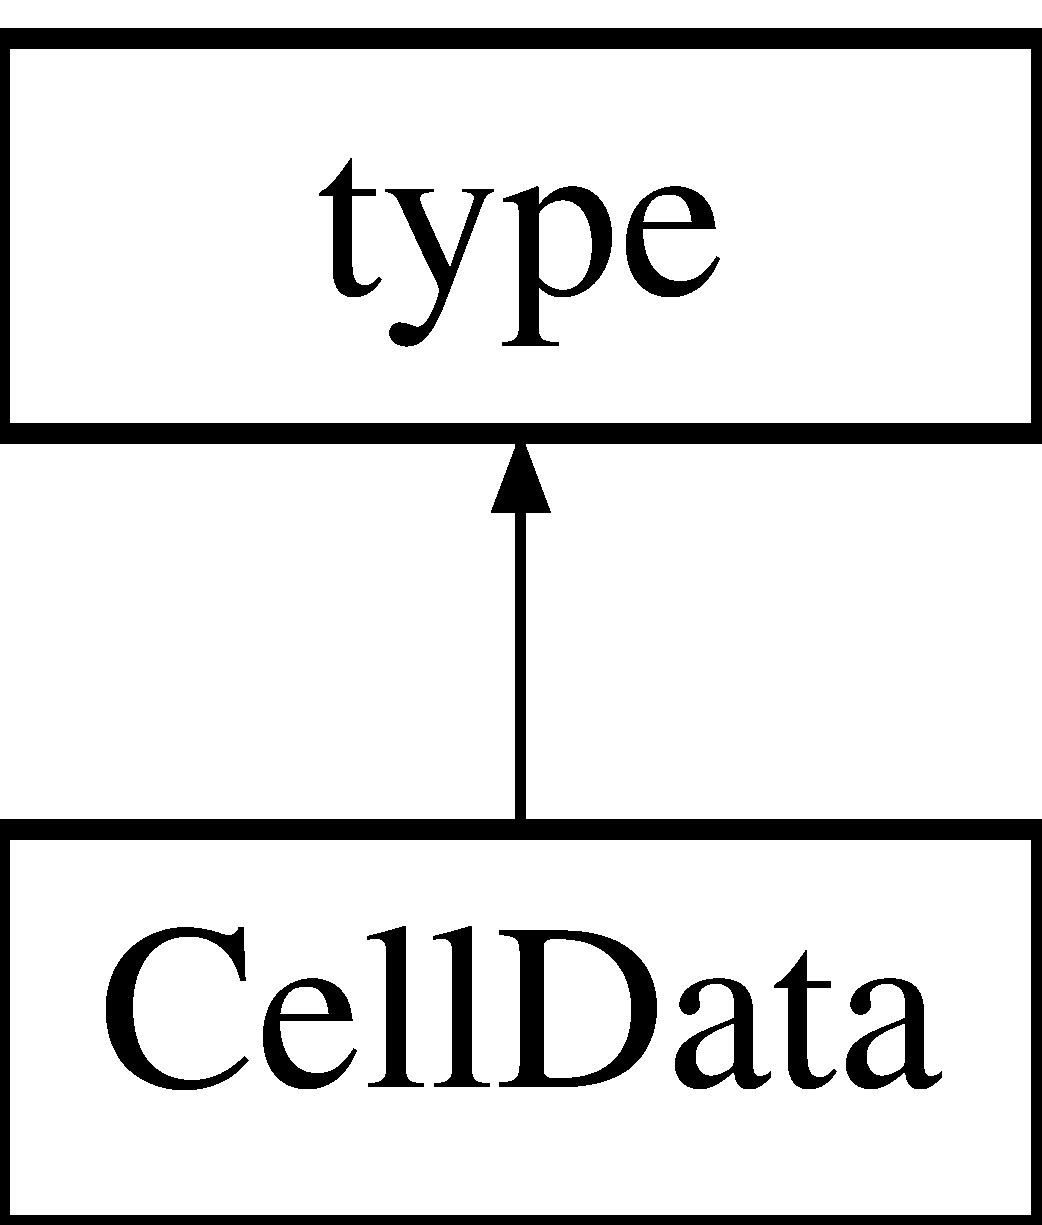
\includegraphics[height=2.000000cm]{classCellData}
\end{center}
\end{figure}
\subsection*{Public Member Functions}
\begin{DoxyCompactItemize}
\item 
virtual \hyperlink{classCellData_aaf439852120aadb5a267799e2a7bf2a3}{$\sim$\+Cell\+Data} ()
\begin{DoxyCompactList}\small\item\em Destructor. \end{DoxyCompactList}\end{DoxyCompactItemize}
\subsection*{Data\+Array}
\label{_amgrp14411195be4ee927801b68cb96397add}%
Accessor and modifier functions for the Data\+Array sequence element. \begin{DoxyCompactItemize}
\item 
typedef \+::\hyperlink{classDataArray__t}{Data\+Array\+\_\+t} \hyperlink{classCellData_a3b277b87cd25225dc944f250bd52057d}{Data\+Array\+\_\+type}
\begin{DoxyCompactList}\small\item\em Element type. \end{DoxyCompactList}\item 
typedef \+::xsd\+::cxx\+::tree\+::sequence$<$ \hyperlink{classCellData_a3b277b87cd25225dc944f250bd52057d}{Data\+Array\+\_\+type} $>$ \hyperlink{classCellData_a52b0c8e18ccdb06ed9e6ae76cd809c4a}{Data\+Array\+\_\+sequence}
\begin{DoxyCompactList}\small\item\em Element sequence container type. \end{DoxyCompactList}\item 
typedef Data\+Array\+\_\+sequence\+::iterator \hyperlink{classCellData_abe0f5b0713690cc81703132bcdccd51f}{Data\+Array\+\_\+iterator}
\begin{DoxyCompactList}\small\item\em Element iterator type. \end{DoxyCompactList}\item 
typedef Data\+Array\+\_\+sequence\+::const\+\_\+iterator \hyperlink{classCellData_a8213ea10f002fac23b5555ca0b2b2a21}{Data\+Array\+\_\+const\+\_\+iterator}
\begin{DoxyCompactList}\small\item\em Element constant iterator type. \end{DoxyCompactList}\item 
typedef \+::xsd\+::cxx\+::tree\+::traits$<$ \hyperlink{classCellData_a3b277b87cd25225dc944f250bd52057d}{Data\+Array\+\_\+type}, char $>$ \hyperlink{classCellData_a03e76eec5af05a6ac5512e9cb80300bd}{Data\+Array\+\_\+traits}
\begin{DoxyCompactList}\small\item\em Element traits type. \end{DoxyCompactList}\item 
const \hyperlink{classCellData_a52b0c8e18ccdb06ed9e6ae76cd809c4a}{Data\+Array\+\_\+sequence} \& \hyperlink{classCellData_af12d2f299905eca541a999dafba1e7e3}{Data\+Array} () const 
\begin{DoxyCompactList}\small\item\em Return a read-\/only (constant) reference to the element sequence. \end{DoxyCompactList}\item 
\hyperlink{classCellData_a52b0c8e18ccdb06ed9e6ae76cd809c4a}{Data\+Array\+\_\+sequence} \& \hyperlink{classCellData_ac40c7e291f83e3e9fabfddeef14131f5}{Data\+Array} ()
\begin{DoxyCompactList}\small\item\em Return a read-\/write reference to the element sequence. \end{DoxyCompactList}\item 
void \hyperlink{classCellData_a9ee9fc1ef295b3ad2c4dc3e9e70ac357}{Data\+Array} (const \hyperlink{classCellData_a52b0c8e18ccdb06ed9e6ae76cd809c4a}{Data\+Array\+\_\+sequence} \&s)
\begin{DoxyCompactList}\small\item\em Copy elements from a given sequence. \end{DoxyCompactList}\end{DoxyCompactItemize}
\subsection*{Constructors}
\begin{DoxyCompactItemize}
\item 
\hyperlink{classCellData_a0d89ba23195659a1fcdc714fa27697a5}{Cell\+Data} ()
\begin{DoxyCompactList}\small\item\em Create an instance from the ultimate base and initializers for required elements and attributes. \end{DoxyCompactList}\item 
\hyperlink{classCellData_ac98b30101e2448016bfa96b9fa6ee18a}{Cell\+Data} (const \+::xercesc\+::\+D\+O\+M\+Element \&e,\+::\hyperlink{namespacexml__schema_a8d981c127a1f5106d04ad5853e707361}{xml\+\_\+schema\+::flags} f=0,\+::\hyperlink{namespacexml__schema_a395f5179c5fc4643909d66e9ff28d8ca}{xml\+\_\+schema\+::container} $\ast$c=0)
\begin{DoxyCompactList}\small\item\em Create an instance from a D\+O\+M element. \end{DoxyCompactList}\item 
\hyperlink{classCellData_ae93656ff9893f518c8f1cfdc611c8045}{Cell\+Data} (const \hyperlink{classCellData}{Cell\+Data} \&x,\+::\hyperlink{namespacexml__schema_a8d981c127a1f5106d04ad5853e707361}{xml\+\_\+schema\+::flags} f=0,\+::\hyperlink{namespacexml__schema_a395f5179c5fc4643909d66e9ff28d8ca}{xml\+\_\+schema\+::container} $\ast$c=0)
\begin{DoxyCompactList}\small\item\em Copy constructor. \end{DoxyCompactList}\item 
virtual \hyperlink{classCellData}{Cell\+Data} $\ast$ \hyperlink{classCellData_aa17c3a153b3a7692dca562878f3fe3ad}{\+\_\+clone} (\+::\hyperlink{namespacexml__schema_a8d981c127a1f5106d04ad5853e707361}{xml\+\_\+schema\+::flags} f=0,\+::\hyperlink{namespacexml__schema_a395f5179c5fc4643909d66e9ff28d8ca}{xml\+\_\+schema\+::container} $\ast$c=0) const 
\begin{DoxyCompactList}\small\item\em Copy the instance polymorphically. \end{DoxyCompactList}\end{DoxyCompactItemize}


\subsection{Detailed Description}
Class corresponding to the Cell\+Data schema type. 

\subsection{Member Typedef Documentation}
\hypertarget{classCellData_a8213ea10f002fac23b5555ca0b2b2a21}{}\index{Cell\+Data@{Cell\+Data}!Data\+Array\+\_\+const\+\_\+iterator@{Data\+Array\+\_\+const\+\_\+iterator}}
\index{Data\+Array\+\_\+const\+\_\+iterator@{Data\+Array\+\_\+const\+\_\+iterator}!Cell\+Data@{Cell\+Data}}
\subsubsection[{Data\+Array\+\_\+const\+\_\+iterator}]{\setlength{\rightskip}{0pt plus 5cm}typedef Data\+Array\+\_\+sequence\+::const\+\_\+iterator {\bf Cell\+Data\+::\+Data\+Array\+\_\+const\+\_\+iterator}}\label{classCellData_a8213ea10f002fac23b5555ca0b2b2a21}


Element constant iterator type. 

\hypertarget{classCellData_abe0f5b0713690cc81703132bcdccd51f}{}\index{Cell\+Data@{Cell\+Data}!Data\+Array\+\_\+iterator@{Data\+Array\+\_\+iterator}}
\index{Data\+Array\+\_\+iterator@{Data\+Array\+\_\+iterator}!Cell\+Data@{Cell\+Data}}
\subsubsection[{Data\+Array\+\_\+iterator}]{\setlength{\rightskip}{0pt plus 5cm}typedef Data\+Array\+\_\+sequence\+::iterator {\bf Cell\+Data\+::\+Data\+Array\+\_\+iterator}}\label{classCellData_abe0f5b0713690cc81703132bcdccd51f}


Element iterator type. 

\hypertarget{classCellData_a52b0c8e18ccdb06ed9e6ae76cd809c4a}{}\index{Cell\+Data@{Cell\+Data}!Data\+Array\+\_\+sequence@{Data\+Array\+\_\+sequence}}
\index{Data\+Array\+\_\+sequence@{Data\+Array\+\_\+sequence}!Cell\+Data@{Cell\+Data}}
\subsubsection[{Data\+Array\+\_\+sequence}]{\setlength{\rightskip}{0pt plus 5cm}typedef \+::xsd\+::cxx\+::tree\+::sequence$<$ {\bf Data\+Array\+\_\+type} $>$ {\bf Cell\+Data\+::\+Data\+Array\+\_\+sequence}}\label{classCellData_a52b0c8e18ccdb06ed9e6ae76cd809c4a}


Element sequence container type. 

\hypertarget{classCellData_a03e76eec5af05a6ac5512e9cb80300bd}{}\index{Cell\+Data@{Cell\+Data}!Data\+Array\+\_\+traits@{Data\+Array\+\_\+traits}}
\index{Data\+Array\+\_\+traits@{Data\+Array\+\_\+traits}!Cell\+Data@{Cell\+Data}}
\subsubsection[{Data\+Array\+\_\+traits}]{\setlength{\rightskip}{0pt plus 5cm}typedef \+::xsd\+::cxx\+::tree\+::traits$<$ {\bf Data\+Array\+\_\+type}, char $>$ {\bf Cell\+Data\+::\+Data\+Array\+\_\+traits}}\label{classCellData_a03e76eec5af05a6ac5512e9cb80300bd}


Element traits type. 

\hypertarget{classCellData_a3b277b87cd25225dc944f250bd52057d}{}\index{Cell\+Data@{Cell\+Data}!Data\+Array\+\_\+type@{Data\+Array\+\_\+type}}
\index{Data\+Array\+\_\+type@{Data\+Array\+\_\+type}!Cell\+Data@{Cell\+Data}}
\subsubsection[{Data\+Array\+\_\+type}]{\setlength{\rightskip}{0pt plus 5cm}typedef \+::{\bf Data\+Array\+\_\+t} {\bf Cell\+Data\+::\+Data\+Array\+\_\+type}}\label{classCellData_a3b277b87cd25225dc944f250bd52057d}


Element type. 



\subsection{Constructor \& Destructor Documentation}
\hypertarget{classCellData_a0d89ba23195659a1fcdc714fa27697a5}{}\index{Cell\+Data@{Cell\+Data}!Cell\+Data@{Cell\+Data}}
\index{Cell\+Data@{Cell\+Data}!Cell\+Data@{Cell\+Data}}
\subsubsection[{Cell\+Data}]{\setlength{\rightskip}{0pt plus 5cm}Cell\+Data\+::\+Cell\+Data (
\begin{DoxyParamCaption}
{}
\end{DoxyParamCaption}
)}\label{classCellData_a0d89ba23195659a1fcdc714fa27697a5}


Create an instance from the ultimate base and initializers for required elements and attributes. 

\hypertarget{classCellData_ac98b30101e2448016bfa96b9fa6ee18a}{}\index{Cell\+Data@{Cell\+Data}!Cell\+Data@{Cell\+Data}}
\index{Cell\+Data@{Cell\+Data}!Cell\+Data@{Cell\+Data}}
\subsubsection[{Cell\+Data}]{\setlength{\rightskip}{0pt plus 5cm}Cell\+Data\+::\+Cell\+Data (
\begin{DoxyParamCaption}
\item[{const \+::xercesc\+::\+D\+O\+M\+Element \&}]{e, }
\item[{\+::{\bf xml\+\_\+schema\+::flags}}]{f = {\ttfamily 0}, }
\item[{\+::{\bf xml\+\_\+schema\+::container} $\ast$}]{c = {\ttfamily 0}}
\end{DoxyParamCaption}
)}\label{classCellData_ac98b30101e2448016bfa96b9fa6ee18a}


Create an instance from a D\+O\+M element. 


\begin{DoxyParams}{Parameters}
{\em e} & A D\+O\+M element to extract the data from. \\
\hline
{\em f} & Flags to create the new instance with. \\
\hline
{\em c} & A pointer to the object that will contain the new instance. \\
\hline
\end{DoxyParams}
\hypertarget{classCellData_ae93656ff9893f518c8f1cfdc611c8045}{}\index{Cell\+Data@{Cell\+Data}!Cell\+Data@{Cell\+Data}}
\index{Cell\+Data@{Cell\+Data}!Cell\+Data@{Cell\+Data}}
\subsubsection[{Cell\+Data}]{\setlength{\rightskip}{0pt plus 5cm}Cell\+Data\+::\+Cell\+Data (
\begin{DoxyParamCaption}
\item[{const {\bf Cell\+Data} \&}]{x, }
\item[{\+::{\bf xml\+\_\+schema\+::flags}}]{f = {\ttfamily 0}, }
\item[{\+::{\bf xml\+\_\+schema\+::container} $\ast$}]{c = {\ttfamily 0}}
\end{DoxyParamCaption}
)}\label{classCellData_ae93656ff9893f518c8f1cfdc611c8045}


Copy constructor. 


\begin{DoxyParams}{Parameters}
{\em x} & An instance to make a copy of. \\
\hline
{\em f} & Flags to create the copy with. \\
\hline
{\em c} & A pointer to the object that will contain the copy.\\
\hline
\end{DoxyParams}
For polymorphic object models use the {\ttfamily \+\_\+clone} function instead. \hypertarget{classCellData_aaf439852120aadb5a267799e2a7bf2a3}{}\index{Cell\+Data@{Cell\+Data}!````~Cell\+Data@{$\sim$\+Cell\+Data}}
\index{````~Cell\+Data@{$\sim$\+Cell\+Data}!Cell\+Data@{Cell\+Data}}
\subsubsection[{$\sim$\+Cell\+Data}]{\setlength{\rightskip}{0pt plus 5cm}Cell\+Data\+::$\sim$\+Cell\+Data (
\begin{DoxyParamCaption}
{}
\end{DoxyParamCaption}
)\hspace{0.3cm}{\ttfamily [virtual]}}\label{classCellData_aaf439852120aadb5a267799e2a7bf2a3}


Destructor. 



\subsection{Member Function Documentation}
\hypertarget{classCellData_aa17c3a153b3a7692dca562878f3fe3ad}{}\index{Cell\+Data@{Cell\+Data}!\+\_\+clone@{\+\_\+clone}}
\index{\+\_\+clone@{\+\_\+clone}!Cell\+Data@{Cell\+Data}}
\subsubsection[{\+\_\+clone}]{\setlength{\rightskip}{0pt plus 5cm}{\bf Cell\+Data} $\ast$ Cell\+Data\+::\+\_\+clone (
\begin{DoxyParamCaption}
\item[{\+::{\bf xml\+\_\+schema\+::flags}}]{f = {\ttfamily 0}, }
\item[{\+::{\bf xml\+\_\+schema\+::container} $\ast$}]{c = {\ttfamily 0}}
\end{DoxyParamCaption}
) const\hspace{0.3cm}{\ttfamily [virtual]}}\label{classCellData_aa17c3a153b3a7692dca562878f3fe3ad}


Copy the instance polymorphically. 


\begin{DoxyParams}{Parameters}
{\em f} & Flags to create the copy with. \\
\hline
{\em c} & A pointer to the object that will contain the copy. \\
\hline
\end{DoxyParams}
\begin{DoxyReturn}{Returns}
A pointer to the dynamically allocated copy.
\end{DoxyReturn}
This function ensures that the dynamic type of the instance is used for copying and should be used for polymorphic object models instead of the copy constructor. \hypertarget{classCellData_af12d2f299905eca541a999dafba1e7e3}{}\index{Cell\+Data@{Cell\+Data}!Data\+Array@{Data\+Array}}
\index{Data\+Array@{Data\+Array}!Cell\+Data@{Cell\+Data}}
\subsubsection[{Data\+Array}]{\setlength{\rightskip}{0pt plus 5cm}const {\bf Cell\+Data\+::\+Data\+Array\+\_\+sequence} \& Cell\+Data\+::\+Data\+Array (
\begin{DoxyParamCaption}
{}
\end{DoxyParamCaption}
) const}\label{classCellData_af12d2f299905eca541a999dafba1e7e3}


Return a read-\/only (constant) reference to the element sequence. 

\begin{DoxyReturn}{Returns}
A constant reference to the sequence container. 
\end{DoxyReturn}
\hypertarget{classCellData_ac40c7e291f83e3e9fabfddeef14131f5}{}\index{Cell\+Data@{Cell\+Data}!Data\+Array@{Data\+Array}}
\index{Data\+Array@{Data\+Array}!Cell\+Data@{Cell\+Data}}
\subsubsection[{Data\+Array}]{\setlength{\rightskip}{0pt plus 5cm}{\bf Cell\+Data\+::\+Data\+Array\+\_\+sequence} \& Cell\+Data\+::\+Data\+Array (
\begin{DoxyParamCaption}
{}
\end{DoxyParamCaption}
)}\label{classCellData_ac40c7e291f83e3e9fabfddeef14131f5}


Return a read-\/write reference to the element sequence. 

\begin{DoxyReturn}{Returns}
A reference to the sequence container. 
\end{DoxyReturn}
\hypertarget{classCellData_a9ee9fc1ef295b3ad2c4dc3e9e70ac357}{}\index{Cell\+Data@{Cell\+Data}!Data\+Array@{Data\+Array}}
\index{Data\+Array@{Data\+Array}!Cell\+Data@{Cell\+Data}}
\subsubsection[{Data\+Array}]{\setlength{\rightskip}{0pt plus 5cm}void Cell\+Data\+::\+Data\+Array (
\begin{DoxyParamCaption}
\item[{const {\bf Data\+Array\+\_\+sequence} \&}]{s}
\end{DoxyParamCaption}
)}\label{classCellData_a9ee9fc1ef295b3ad2c4dc3e9e70ac357}


Copy elements from a given sequence. 


\begin{DoxyParams}{Parameters}
{\em s} & A sequence to copy elements from.\\
\hline
\end{DoxyParams}
For each element in {\itshape s} this function makes a copy and adds it to the sequence. Note that this operation completely changes the sequence and all old elements will be lost. 

The documentation for this class was generated from the following files\+:\begin{DoxyCompactItemize}
\item 
src/output\+Writer/\hyperlink{vtk-unstructured_8h}{vtk-\/unstructured.\+h}\item 
src/output\+Writer/\hyperlink{vtk-unstructured_8cpp}{vtk-\/unstructured.\+cpp}\end{DoxyCompactItemize}

\hypertarget{classCells}{}\section{Cells Class Reference}
\label{classCells}\index{Cells@{Cells}}


Class corresponding to the Cells schema type.  




{\ttfamily \#include $<$vtk-\/unstructured.\+h$>$}

Inheritance diagram for Cells\+:\begin{figure}[H]
\begin{center}
\leavevmode
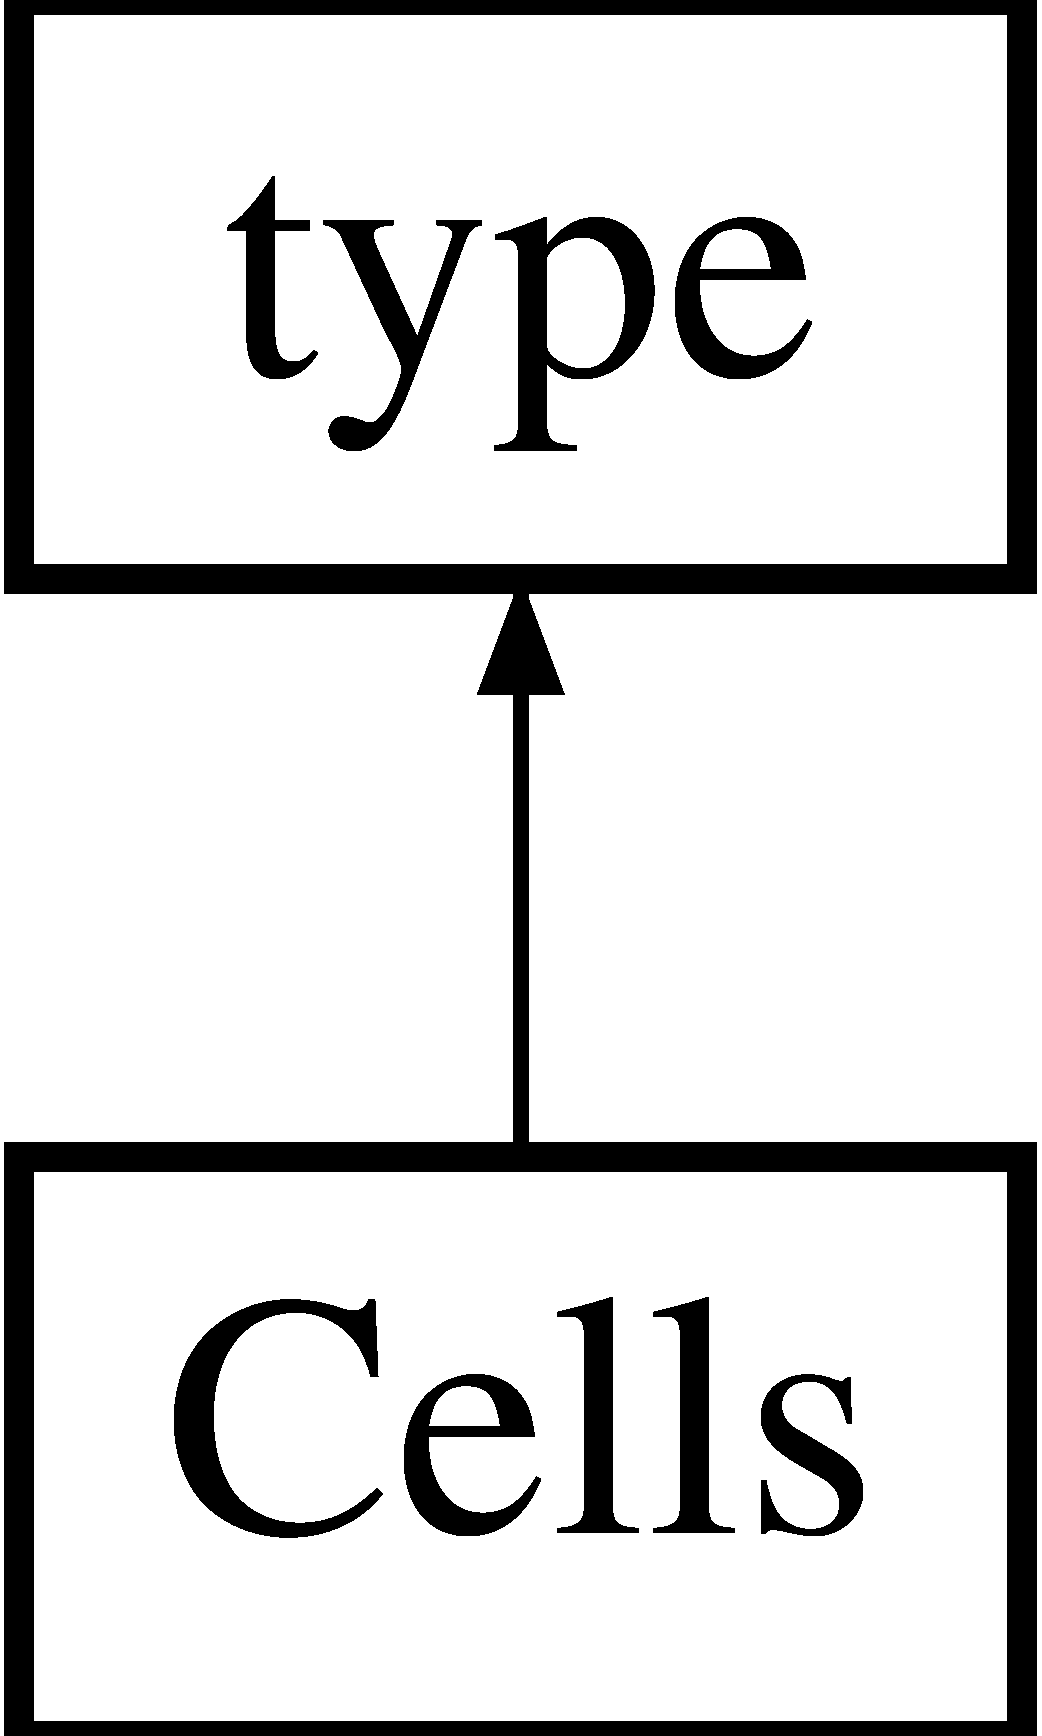
\includegraphics[height=2.000000cm]{classCells}
\end{center}
\end{figure}
\subsection*{Public Member Functions}
\begin{DoxyCompactItemize}
\item 
virtual \hyperlink{classCells_aab121634db81b439226a33fd099fb3c1}{$\sim$\+Cells} ()
\begin{DoxyCompactList}\small\item\em Destructor. \end{DoxyCompactList}\end{DoxyCompactItemize}
\subsection*{Data\+Array}
\label{_amgrp14411195be4ee927801b68cb96397add}%
Accessor and modifier functions for the Data\+Array sequence element. \begin{DoxyCompactItemize}
\item 
typedef \+::\hyperlink{classDataArray__t}{Data\+Array\+\_\+t} \hyperlink{classCells_ad69e76337c22596e70b27d93c54dd722}{Data\+Array\+\_\+type}
\begin{DoxyCompactList}\small\item\em Element type. \end{DoxyCompactList}\item 
typedef \+::xsd\+::cxx\+::tree\+::sequence$<$ \hyperlink{classCells_ad69e76337c22596e70b27d93c54dd722}{Data\+Array\+\_\+type} $>$ \hyperlink{classCells_ae2856ec1cc2c6d6a2ccac9de9a22c7b7}{Data\+Array\+\_\+sequence}
\begin{DoxyCompactList}\small\item\em Element sequence container type. \end{DoxyCompactList}\item 
typedef Data\+Array\+\_\+sequence\+::iterator \hyperlink{classCells_a1873efdee2bb668676d01a7a5010faa2}{Data\+Array\+\_\+iterator}
\begin{DoxyCompactList}\small\item\em Element iterator type. \end{DoxyCompactList}\item 
typedef Data\+Array\+\_\+sequence\+::const\+\_\+iterator \hyperlink{classCells_ad01c81703074599471cd6159cdea1ac1}{Data\+Array\+\_\+const\+\_\+iterator}
\begin{DoxyCompactList}\small\item\em Element constant iterator type. \end{DoxyCompactList}\item 
typedef \+::xsd\+::cxx\+::tree\+::traits$<$ \hyperlink{classCells_ad69e76337c22596e70b27d93c54dd722}{Data\+Array\+\_\+type}, char $>$ \hyperlink{classCells_ac35ecebe10914f3d35e85589e998462b}{Data\+Array\+\_\+traits}
\begin{DoxyCompactList}\small\item\em Element traits type. \end{DoxyCompactList}\item 
const \hyperlink{classCells_ae2856ec1cc2c6d6a2ccac9de9a22c7b7}{Data\+Array\+\_\+sequence} \& \hyperlink{classCells_a8844f4f5a352181f29e8589d72fba69f}{Data\+Array} () const 
\begin{DoxyCompactList}\small\item\em Return a read-\/only (constant) reference to the element sequence. \end{DoxyCompactList}\item 
\hyperlink{classCells_ae2856ec1cc2c6d6a2ccac9de9a22c7b7}{Data\+Array\+\_\+sequence} \& \hyperlink{classCells_a6114566d42273127f9cb92b1d0f09cb5}{Data\+Array} ()
\begin{DoxyCompactList}\small\item\em Return a read-\/write reference to the element sequence. \end{DoxyCompactList}\item 
void \hyperlink{classCells_a52c9971e15358118dd90ecf68b26601e}{Data\+Array} (const \hyperlink{classCells_ae2856ec1cc2c6d6a2ccac9de9a22c7b7}{Data\+Array\+\_\+sequence} \&s)
\begin{DoxyCompactList}\small\item\em Copy elements from a given sequence. \end{DoxyCompactList}\end{DoxyCompactItemize}
\subsection*{Constructors}
\begin{DoxyCompactItemize}
\item 
\hyperlink{classCells_a092d62bc15648a54755a413dbf9a2db0}{Cells} ()
\begin{DoxyCompactList}\small\item\em Create an instance from the ultimate base and initializers for required elements and attributes. \end{DoxyCompactList}\item 
\hyperlink{classCells_a79e3031094d928c8d275198201d44f0c}{Cells} (const \+::xercesc\+::\+D\+O\+M\+Element \&e,\+::\hyperlink{namespacexml__schema_a8d981c127a1f5106d04ad5853e707361}{xml\+\_\+schema\+::flags} f=0,\+::\hyperlink{namespacexml__schema_a395f5179c5fc4643909d66e9ff28d8ca}{xml\+\_\+schema\+::container} $\ast$c=0)
\begin{DoxyCompactList}\small\item\em Create an instance from a D\+O\+M element. \end{DoxyCompactList}\item 
\hyperlink{classCells_a9322653263fb302eb7068be10b1b364f}{Cells} (const \hyperlink{classCells}{Cells} \&x,\+::\hyperlink{namespacexml__schema_a8d981c127a1f5106d04ad5853e707361}{xml\+\_\+schema\+::flags} f=0,\+::\hyperlink{namespacexml__schema_a395f5179c5fc4643909d66e9ff28d8ca}{xml\+\_\+schema\+::container} $\ast$c=0)
\begin{DoxyCompactList}\small\item\em Copy constructor. \end{DoxyCompactList}\item 
virtual \hyperlink{classCells}{Cells} $\ast$ \hyperlink{classCells_a67e7fa1cc404dcc4814011ca179f8a83}{\+\_\+clone} (\+::\hyperlink{namespacexml__schema_a8d981c127a1f5106d04ad5853e707361}{xml\+\_\+schema\+::flags} f=0,\+::\hyperlink{namespacexml__schema_a395f5179c5fc4643909d66e9ff28d8ca}{xml\+\_\+schema\+::container} $\ast$c=0) const 
\begin{DoxyCompactList}\small\item\em Copy the instance polymorphically. \end{DoxyCompactList}\end{DoxyCompactItemize}


\subsection{Detailed Description}
Class corresponding to the Cells schema type. 

\subsection{Member Typedef Documentation}
\hypertarget{classCells_ad01c81703074599471cd6159cdea1ac1}{}\index{Cells@{Cells}!Data\+Array\+\_\+const\+\_\+iterator@{Data\+Array\+\_\+const\+\_\+iterator}}
\index{Data\+Array\+\_\+const\+\_\+iterator@{Data\+Array\+\_\+const\+\_\+iterator}!Cells@{Cells}}
\subsubsection[{Data\+Array\+\_\+const\+\_\+iterator}]{\setlength{\rightskip}{0pt plus 5cm}typedef Data\+Array\+\_\+sequence\+::const\+\_\+iterator {\bf Cells\+::\+Data\+Array\+\_\+const\+\_\+iterator}}\label{classCells_ad01c81703074599471cd6159cdea1ac1}


Element constant iterator type. 

\hypertarget{classCells_a1873efdee2bb668676d01a7a5010faa2}{}\index{Cells@{Cells}!Data\+Array\+\_\+iterator@{Data\+Array\+\_\+iterator}}
\index{Data\+Array\+\_\+iterator@{Data\+Array\+\_\+iterator}!Cells@{Cells}}
\subsubsection[{Data\+Array\+\_\+iterator}]{\setlength{\rightskip}{0pt plus 5cm}typedef Data\+Array\+\_\+sequence\+::iterator {\bf Cells\+::\+Data\+Array\+\_\+iterator}}\label{classCells_a1873efdee2bb668676d01a7a5010faa2}


Element iterator type. 

\hypertarget{classCells_ae2856ec1cc2c6d6a2ccac9de9a22c7b7}{}\index{Cells@{Cells}!Data\+Array\+\_\+sequence@{Data\+Array\+\_\+sequence}}
\index{Data\+Array\+\_\+sequence@{Data\+Array\+\_\+sequence}!Cells@{Cells}}
\subsubsection[{Data\+Array\+\_\+sequence}]{\setlength{\rightskip}{0pt plus 5cm}typedef \+::xsd\+::cxx\+::tree\+::sequence$<$ {\bf Data\+Array\+\_\+type} $>$ {\bf Cells\+::\+Data\+Array\+\_\+sequence}}\label{classCells_ae2856ec1cc2c6d6a2ccac9de9a22c7b7}


Element sequence container type. 

\hypertarget{classCells_ac35ecebe10914f3d35e85589e998462b}{}\index{Cells@{Cells}!Data\+Array\+\_\+traits@{Data\+Array\+\_\+traits}}
\index{Data\+Array\+\_\+traits@{Data\+Array\+\_\+traits}!Cells@{Cells}}
\subsubsection[{Data\+Array\+\_\+traits}]{\setlength{\rightskip}{0pt plus 5cm}typedef \+::xsd\+::cxx\+::tree\+::traits$<$ {\bf Data\+Array\+\_\+type}, char $>$ {\bf Cells\+::\+Data\+Array\+\_\+traits}}\label{classCells_ac35ecebe10914f3d35e85589e998462b}


Element traits type. 

\hypertarget{classCells_ad69e76337c22596e70b27d93c54dd722}{}\index{Cells@{Cells}!Data\+Array\+\_\+type@{Data\+Array\+\_\+type}}
\index{Data\+Array\+\_\+type@{Data\+Array\+\_\+type}!Cells@{Cells}}
\subsubsection[{Data\+Array\+\_\+type}]{\setlength{\rightskip}{0pt plus 5cm}typedef \+::{\bf Data\+Array\+\_\+t} {\bf Cells\+::\+Data\+Array\+\_\+type}}\label{classCells_ad69e76337c22596e70b27d93c54dd722}


Element type. 



\subsection{Constructor \& Destructor Documentation}
\hypertarget{classCells_a092d62bc15648a54755a413dbf9a2db0}{}\index{Cells@{Cells}!Cells@{Cells}}
\index{Cells@{Cells}!Cells@{Cells}}
\subsubsection[{Cells}]{\setlength{\rightskip}{0pt plus 5cm}Cells\+::\+Cells (
\begin{DoxyParamCaption}
{}
\end{DoxyParamCaption}
)}\label{classCells_a092d62bc15648a54755a413dbf9a2db0}


Create an instance from the ultimate base and initializers for required elements and attributes. 

\hypertarget{classCells_a79e3031094d928c8d275198201d44f0c}{}\index{Cells@{Cells}!Cells@{Cells}}
\index{Cells@{Cells}!Cells@{Cells}}
\subsubsection[{Cells}]{\setlength{\rightskip}{0pt plus 5cm}Cells\+::\+Cells (
\begin{DoxyParamCaption}
\item[{const \+::xercesc\+::\+D\+O\+M\+Element \&}]{e, }
\item[{\+::{\bf xml\+\_\+schema\+::flags}}]{f = {\ttfamily 0}, }
\item[{\+::{\bf xml\+\_\+schema\+::container} $\ast$}]{c = {\ttfamily 0}}
\end{DoxyParamCaption}
)}\label{classCells_a79e3031094d928c8d275198201d44f0c}


Create an instance from a D\+O\+M element. 


\begin{DoxyParams}{Parameters}
{\em e} & A D\+O\+M element to extract the data from. \\
\hline
{\em f} & Flags to create the new instance with. \\
\hline
{\em c} & A pointer to the object that will contain the new instance. \\
\hline
\end{DoxyParams}
\hypertarget{classCells_a9322653263fb302eb7068be10b1b364f}{}\index{Cells@{Cells}!Cells@{Cells}}
\index{Cells@{Cells}!Cells@{Cells}}
\subsubsection[{Cells}]{\setlength{\rightskip}{0pt plus 5cm}Cells\+::\+Cells (
\begin{DoxyParamCaption}
\item[{const {\bf Cells} \&}]{x, }
\item[{\+::{\bf xml\+\_\+schema\+::flags}}]{f = {\ttfamily 0}, }
\item[{\+::{\bf xml\+\_\+schema\+::container} $\ast$}]{c = {\ttfamily 0}}
\end{DoxyParamCaption}
)}\label{classCells_a9322653263fb302eb7068be10b1b364f}


Copy constructor. 


\begin{DoxyParams}{Parameters}
{\em x} & An instance to make a copy of. \\
\hline
{\em f} & Flags to create the copy with. \\
\hline
{\em c} & A pointer to the object that will contain the copy.\\
\hline
\end{DoxyParams}
For polymorphic object models use the {\ttfamily \+\_\+clone} function instead. \hypertarget{classCells_aab121634db81b439226a33fd099fb3c1}{}\index{Cells@{Cells}!````~Cells@{$\sim$\+Cells}}
\index{````~Cells@{$\sim$\+Cells}!Cells@{Cells}}
\subsubsection[{$\sim$\+Cells}]{\setlength{\rightskip}{0pt plus 5cm}Cells\+::$\sim$\+Cells (
\begin{DoxyParamCaption}
{}
\end{DoxyParamCaption}
)\hspace{0.3cm}{\ttfamily [virtual]}}\label{classCells_aab121634db81b439226a33fd099fb3c1}


Destructor. 



\subsection{Member Function Documentation}
\hypertarget{classCells_a67e7fa1cc404dcc4814011ca179f8a83}{}\index{Cells@{Cells}!\+\_\+clone@{\+\_\+clone}}
\index{\+\_\+clone@{\+\_\+clone}!Cells@{Cells}}
\subsubsection[{\+\_\+clone}]{\setlength{\rightskip}{0pt plus 5cm}{\bf Cells} $\ast$ Cells\+::\+\_\+clone (
\begin{DoxyParamCaption}
\item[{\+::{\bf xml\+\_\+schema\+::flags}}]{f = {\ttfamily 0}, }
\item[{\+::{\bf xml\+\_\+schema\+::container} $\ast$}]{c = {\ttfamily 0}}
\end{DoxyParamCaption}
) const\hspace{0.3cm}{\ttfamily [virtual]}}\label{classCells_a67e7fa1cc404dcc4814011ca179f8a83}


Copy the instance polymorphically. 


\begin{DoxyParams}{Parameters}
{\em f} & Flags to create the copy with. \\
\hline
{\em c} & A pointer to the object that will contain the copy. \\
\hline
\end{DoxyParams}
\begin{DoxyReturn}{Returns}
A pointer to the dynamically allocated copy.
\end{DoxyReturn}
This function ensures that the dynamic type of the instance is used for copying and should be used for polymorphic object models instead of the copy constructor. \hypertarget{classCells_a8844f4f5a352181f29e8589d72fba69f}{}\index{Cells@{Cells}!Data\+Array@{Data\+Array}}
\index{Data\+Array@{Data\+Array}!Cells@{Cells}}
\subsubsection[{Data\+Array}]{\setlength{\rightskip}{0pt plus 5cm}const {\bf Cells\+::\+Data\+Array\+\_\+sequence} \& Cells\+::\+Data\+Array (
\begin{DoxyParamCaption}
{}
\end{DoxyParamCaption}
) const}\label{classCells_a8844f4f5a352181f29e8589d72fba69f}


Return a read-\/only (constant) reference to the element sequence. 

\begin{DoxyReturn}{Returns}
A constant reference to the sequence container. 
\end{DoxyReturn}
\hypertarget{classCells_a6114566d42273127f9cb92b1d0f09cb5}{}\index{Cells@{Cells}!Data\+Array@{Data\+Array}}
\index{Data\+Array@{Data\+Array}!Cells@{Cells}}
\subsubsection[{Data\+Array}]{\setlength{\rightskip}{0pt plus 5cm}{\bf Cells\+::\+Data\+Array\+\_\+sequence} \& Cells\+::\+Data\+Array (
\begin{DoxyParamCaption}
{}
\end{DoxyParamCaption}
)}\label{classCells_a6114566d42273127f9cb92b1d0f09cb5}


Return a read-\/write reference to the element sequence. 

\begin{DoxyReturn}{Returns}
A reference to the sequence container. 
\end{DoxyReturn}
\hypertarget{classCells_a52c9971e15358118dd90ecf68b26601e}{}\index{Cells@{Cells}!Data\+Array@{Data\+Array}}
\index{Data\+Array@{Data\+Array}!Cells@{Cells}}
\subsubsection[{Data\+Array}]{\setlength{\rightskip}{0pt plus 5cm}void Cells\+::\+Data\+Array (
\begin{DoxyParamCaption}
\item[{const {\bf Data\+Array\+\_\+sequence} \&}]{s}
\end{DoxyParamCaption}
)}\label{classCells_a52c9971e15358118dd90ecf68b26601e}


Copy elements from a given sequence. 


\begin{DoxyParams}{Parameters}
{\em s} & A sequence to copy elements from.\\
\hline
\end{DoxyParams}
For each element in {\itshape s} this function makes a copy and adds it to the sequence. Note that this operation completely changes the sequence and all old elements will be lost. 

The documentation for this class was generated from the following files\+:\begin{DoxyCompactItemize}
\item 
src/output\+Writer/\hyperlink{vtk-unstructured_8h}{vtk-\/unstructured.\+h}\item 
src/output\+Writer/\hyperlink{vtk-unstructured_8cpp}{vtk-\/unstructured.\+cpp}\end{DoxyCompactItemize}

\hypertarget{classDataArray__t}{}\section{Data\+Array\+\_\+t Class Reference}
\label{classDataArray__t}\index{Data\+Array\+\_\+t@{Data\+Array\+\_\+t}}


Class corresponding to the Data\+Array\+\_\+t schema type.  




{\ttfamily \#include $<$vtk-\/unstructured.\+h$>$}

Inheritance diagram for Data\+Array\+\_\+t\+:\begin{figure}[H]
\begin{center}
\leavevmode
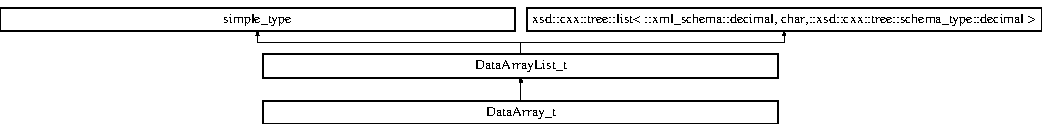
\includegraphics[height=1.660079cm]{classDataArray__t}
\end{center}
\end{figure}
\subsection*{Public Member Functions}
\begin{DoxyCompactItemize}
\item 
virtual \hyperlink{classDataArray__t_ac9806a5eedf7abecd7adf6408c8af894}{$\sim$\+Data\+Array\+\_\+t} ()
\begin{DoxyCompactList}\small\item\em Destructor. \end{DoxyCompactList}\end{DoxyCompactItemize}
\subsection*{type}
\label{_amgrp599dcce2998a6b40b1e38e8c6006cb0a}%
Accessor and modifier functions for the type required attribute. \begin{DoxyCompactItemize}
\item 
typedef \+::\hyperlink{classtype}{type} \hyperlink{classDataArray__t_a484a0509e4f141d9970d75881703a51e}{type\+\_\+type}
\begin{DoxyCompactList}\small\item\em Attribute type. \end{DoxyCompactList}\item 
typedef \+::xsd\+::cxx\+::tree\+::traits$<$ \hyperlink{classDataArray__t_a484a0509e4f141d9970d75881703a51e}{type\+\_\+type}, char $>$ \hyperlink{classDataArray__t_af1dc5f097a8645ae42b57eb3a0b10fa2}{type\+\_\+traits}
\begin{DoxyCompactList}\small\item\em Attribute traits type. \end{DoxyCompactList}\item 
const \hyperlink{classDataArray__t_a484a0509e4f141d9970d75881703a51e}{type\+\_\+type} \& \hyperlink{classDataArray__t_a6ec3c246d1a2fddc7052bcde2cb6bdf7}{type} () const 
\begin{DoxyCompactList}\small\item\em Return a read-\/only (constant) reference to the attribute. \end{DoxyCompactList}\item 
\hyperlink{classDataArray__t_a484a0509e4f141d9970d75881703a51e}{type\+\_\+type} \& \hyperlink{classDataArray__t_a29f3ed42a5bf8df9437ece5f63c02301}{type} ()
\begin{DoxyCompactList}\small\item\em Return a read-\/write reference to the attribute. \end{DoxyCompactList}\item 
void \hyperlink{classDataArray__t_ae4fd6c47e992055ec42cc1949b60da2a}{type} (const \hyperlink{classDataArray__t_a484a0509e4f141d9970d75881703a51e}{type\+\_\+type} \&x)
\begin{DoxyCompactList}\small\item\em Set the attribute value. \end{DoxyCompactList}\item 
void \hyperlink{classDataArray__t_afa90d226889ba3e7baa5c8e9dba594d2}{type} (\+::std\+::auto\+\_\+ptr$<$ \hyperlink{classDataArray__t_a484a0509e4f141d9970d75881703a51e}{type\+\_\+type} $>$ p)
\begin{DoxyCompactList}\small\item\em Set the attribute value without copying. \end{DoxyCompactList}\end{DoxyCompactItemize}
\subsection*{Name}
\label{_amgrp49ee3087348e8d44e1feda1917443987}%
Accessor and modifier functions for the Name required attribute. \begin{DoxyCompactItemize}
\item 
typedef \+::\hyperlink{namespacexml__schema_aefbaf353f9a0043af46d23d9040ef268}{xml\+\_\+schema\+::string} \hyperlink{classDataArray__t_afc6836923916c2489f91caea78ec4ad6}{Name\+\_\+type}
\begin{DoxyCompactList}\small\item\em Attribute type. \end{DoxyCompactList}\item 
typedef \+::xsd\+::cxx\+::tree\+::traits$<$ \hyperlink{classDataArray__t_afc6836923916c2489f91caea78ec4ad6}{Name\+\_\+type}, char $>$ \hyperlink{classDataArray__t_a46d0b4cf44ee9122e4cbb3bd3abe6663}{Name\+\_\+traits}
\begin{DoxyCompactList}\small\item\em Attribute traits type. \end{DoxyCompactList}\item 
const \hyperlink{classDataArray__t_afc6836923916c2489f91caea78ec4ad6}{Name\+\_\+type} \& \hyperlink{classDataArray__t_ada03ebff820f73d64d0761a0fb977527}{Name} () const 
\begin{DoxyCompactList}\small\item\em Return a read-\/only (constant) reference to the attribute. \end{DoxyCompactList}\item 
\hyperlink{classDataArray__t_afc6836923916c2489f91caea78ec4ad6}{Name\+\_\+type} \& \hyperlink{classDataArray__t_aeb126f8a8b03eea44eed5a2b606da59c}{Name} ()
\begin{DoxyCompactList}\small\item\em Return a read-\/write reference to the attribute. \end{DoxyCompactList}\item 
void \hyperlink{classDataArray__t_a95a1f49a6dd9f54fb71fb6b70240a51b}{Name} (const \hyperlink{classDataArray__t_afc6836923916c2489f91caea78ec4ad6}{Name\+\_\+type} \&x)
\begin{DoxyCompactList}\small\item\em Set the attribute value. \end{DoxyCompactList}\item 
void \hyperlink{classDataArray__t_a290f1b5702b7a623a0c9fc086a7a0d0c}{Name} (\+::std\+::auto\+\_\+ptr$<$ \hyperlink{classDataArray__t_afc6836923916c2489f91caea78ec4ad6}{Name\+\_\+type} $>$ p)
\begin{DoxyCompactList}\small\item\em Set the attribute value without copying. \end{DoxyCompactList}\end{DoxyCompactItemize}
\subsection*{Number\+Of\+Components}
\label{_amgrp2a0e258c3f78050b74e96bb0ed643748}%
Accessor and modifier functions for the Number\+Of\+Components required attribute. \begin{DoxyCompactItemize}
\item 
typedef \+::\hyperlink{namespacexml__schema_aaaea7c8ce4dfbe26cc52c91c29c97b7c}{xml\+\_\+schema\+::integer} \hyperlink{classDataArray__t_aac602cec132f6e771f7fa3be1d19c16f}{Number\+Of\+Components\+\_\+type}
\begin{DoxyCompactList}\small\item\em Attribute type. \end{DoxyCompactList}\item 
typedef \+::xsd\+::cxx\+::tree\+::traits$<$ \hyperlink{classDataArray__t_aac602cec132f6e771f7fa3be1d19c16f}{Number\+Of\+Components\+\_\+type}, char $>$ \hyperlink{classDataArray__t_a1112148f87db2c0ba05323377d9f0427}{Number\+Of\+Components\+\_\+traits}
\begin{DoxyCompactList}\small\item\em Attribute traits type. \end{DoxyCompactList}\item 
const \hyperlink{classDataArray__t_aac602cec132f6e771f7fa3be1d19c16f}{Number\+Of\+Components\+\_\+type} \& \hyperlink{classDataArray__t_a715a5b58a694d49499591bfea3a282ae}{Number\+Of\+Components} () const 
\begin{DoxyCompactList}\small\item\em Return a read-\/only (constant) reference to the attribute. \end{DoxyCompactList}\item 
\hyperlink{classDataArray__t_aac602cec132f6e771f7fa3be1d19c16f}{Number\+Of\+Components\+\_\+type} \& \hyperlink{classDataArray__t_a6f80fc5ce05d51d4292c698464d4ace3}{Number\+Of\+Components} ()
\begin{DoxyCompactList}\small\item\em Return a read-\/write reference to the attribute. \end{DoxyCompactList}\item 
void \hyperlink{classDataArray__t_a755fae9b31318f98a3d21beba16f2841}{Number\+Of\+Components} (const \hyperlink{classDataArray__t_aac602cec132f6e771f7fa3be1d19c16f}{Number\+Of\+Components\+\_\+type} \&x)
\begin{DoxyCompactList}\small\item\em Set the attribute value. \end{DoxyCompactList}\end{DoxyCompactItemize}
\subsection*{format}
\label{_amgrp1ddcb92ade31c8fbd370001f9b29a7d9}%
Accessor and modifier functions for the format optional attribute with a default value. \begin{DoxyCompactItemize}
\item 
typedef \+::\hyperlink{namespacexml__schema_aefbaf353f9a0043af46d23d9040ef268}{xml\+\_\+schema\+::string} \hyperlink{classDataArray__t_ae453ea653980baef2e3296005d70bfbd}{format\+\_\+type}
\begin{DoxyCompactList}\small\item\em Attribute type. \end{DoxyCompactList}\item 
typedef \+::xsd\+::cxx\+::tree\+::traits$<$ \hyperlink{classDataArray__t_ae453ea653980baef2e3296005d70bfbd}{format\+\_\+type}, char $>$ \hyperlink{classDataArray__t_a2a31ef3ce1dfa973843a02e17762e7a3}{format\+\_\+traits}
\begin{DoxyCompactList}\small\item\em Attribute traits type. \end{DoxyCompactList}\item 
const \hyperlink{classDataArray__t_ae453ea653980baef2e3296005d70bfbd}{format\+\_\+type} \& \hyperlink{classDataArray__t_a7a39cab4205282736e633d8a3c57bbae}{format} () const 
\begin{DoxyCompactList}\small\item\em Return a read-\/only (constant) reference to the attribute. \end{DoxyCompactList}\item 
static const \hyperlink{classDataArray__t_ae453ea653980baef2e3296005d70bfbd}{format\+\_\+type} \& \hyperlink{classDataArray__t_ade99ea2c2fdc45cc2826b6847dfb5404}{format\+\_\+default\+\_\+value} ()
\begin{DoxyCompactList}\small\item\em Return the default value for the attribute. \end{DoxyCompactList}\end{DoxyCompactItemize}
\subsection*{offset}
\label{_amgrp7a86c157ee9713c34fbd7a1ee40f0c5a}%
Accessor and modifier functions for the offset optional attribute. \begin{DoxyCompactItemize}
\item 
typedef \+::\hyperlink{namespacexml__schema_aaaea7c8ce4dfbe26cc52c91c29c97b7c}{xml\+\_\+schema\+::integer} \hyperlink{classDataArray__t_a7b840c5f08bd2c65cd3c5e24ad132cfb}{offset\+\_\+type}
\begin{DoxyCompactList}\small\item\em Attribute type. \end{DoxyCompactList}\item 
typedef \+::xsd\+::cxx\+::tree\+::optional$<$ \hyperlink{classDataArray__t_a7b840c5f08bd2c65cd3c5e24ad132cfb}{offset\+\_\+type} $>$ \hyperlink{classDataArray__t_a4bc33060e7c386b658c752347ac5f03e}{offset\+\_\+optional}
\begin{DoxyCompactList}\small\item\em Attribute optional container type. \end{DoxyCompactList}\item 
typedef \+::xsd\+::cxx\+::tree\+::traits$<$ \hyperlink{classDataArray__t_a7b840c5f08bd2c65cd3c5e24ad132cfb}{offset\+\_\+type}, char $>$ \hyperlink{classDataArray__t_a2e3e1a5de665fc64a3d86fd94bb1af0f}{offset\+\_\+traits}
\begin{DoxyCompactList}\small\item\em Attribute traits type. \end{DoxyCompactList}\item 
const \hyperlink{classDataArray__t_a4bc33060e7c386b658c752347ac5f03e}{offset\+\_\+optional} \& \hyperlink{classDataArray__t_a995d24c5c7a88929a6b0e7de154bbdf5}{offset} () const 
\begin{DoxyCompactList}\small\item\em Return a read-\/only (constant) reference to the attribute container. \end{DoxyCompactList}\item 
\hyperlink{classDataArray__t_a4bc33060e7c386b658c752347ac5f03e}{offset\+\_\+optional} \& \hyperlink{classDataArray__t_aed72cbf5f3476360f4898f487a074c26}{offset} ()
\begin{DoxyCompactList}\small\item\em Return a read-\/write reference to the attribute container. \end{DoxyCompactList}\item 
void \hyperlink{classDataArray__t_ac133def4ed8ae6c623d0144f036a18d7}{offset} (const \hyperlink{classDataArray__t_a7b840c5f08bd2c65cd3c5e24ad132cfb}{offset\+\_\+type} \&x)
\begin{DoxyCompactList}\small\item\em Set the attribute value. \end{DoxyCompactList}\item 
void \hyperlink{classDataArray__t_a5abb95d7ab6fb95015c06de57a6ccbc9}{offset} (const \hyperlink{classDataArray__t_a4bc33060e7c386b658c752347ac5f03e}{offset\+\_\+optional} \&x)
\begin{DoxyCompactList}\small\item\em Set the attribute value. \end{DoxyCompactList}\end{DoxyCompactItemize}
\subsection*{Constructors}
\begin{DoxyCompactItemize}
\item 
\hyperlink{classDataArray__t_a0700e9e63538064c2f9eb668fe3ca624}{Data\+Array\+\_\+t} (const \hyperlink{classDataArray__t_a484a0509e4f141d9970d75881703a51e}{type\+\_\+type} \&, const \hyperlink{classDataArray__t_afc6836923916c2489f91caea78ec4ad6}{Name\+\_\+type} \&, const \hyperlink{classDataArray__t_aac602cec132f6e771f7fa3be1d19c16f}{Number\+Of\+Components\+\_\+type} \&)
\begin{DoxyCompactList}\small\item\em Create an instance from initializers for required elements and attributes. \end{DoxyCompactList}\item 
\hyperlink{classDataArray__t_a3c07c46f9c607ce6da2d2e456494465a}{Data\+Array\+\_\+t} (const \+::\hyperlink{classDataArrayList__t}{Data\+Array\+List\+\_\+t} \&, const \hyperlink{classDataArray__t_a484a0509e4f141d9970d75881703a51e}{type\+\_\+type} \&, const \hyperlink{classDataArray__t_afc6836923916c2489f91caea78ec4ad6}{Name\+\_\+type} \&, const \hyperlink{classDataArray__t_aac602cec132f6e771f7fa3be1d19c16f}{Number\+Of\+Components\+\_\+type} \&)
\begin{DoxyCompactList}\small\item\em Create an instance from the ultimate base and initializers for required elements and attributes. \end{DoxyCompactList}\item 
\hyperlink{classDataArray__t_ae02d07853318c1d754e0acfc80f5c894}{Data\+Array\+\_\+t} (const \+::xercesc\+::\+D\+O\+M\+Element \&e,\+::\hyperlink{namespacexml__schema_a8d981c127a1f5106d04ad5853e707361}{xml\+\_\+schema\+::flags} f=0,\+::\hyperlink{namespacexml__schema_a395f5179c5fc4643909d66e9ff28d8ca}{xml\+\_\+schema\+::container} $\ast$c=0)
\begin{DoxyCompactList}\small\item\em Create an instance from a D\+O\+M element. \end{DoxyCompactList}\item 
\hyperlink{classDataArray__t_a6f67fee4225ca87492d8496de4121de7}{Data\+Array\+\_\+t} (const \hyperlink{classDataArray__t}{Data\+Array\+\_\+t} \&x,\+::\hyperlink{namespacexml__schema_a8d981c127a1f5106d04ad5853e707361}{xml\+\_\+schema\+::flags} f=0,\+::\hyperlink{namespacexml__schema_a395f5179c5fc4643909d66e9ff28d8ca}{xml\+\_\+schema\+::container} $\ast$c=0)
\begin{DoxyCompactList}\small\item\em Copy constructor. \end{DoxyCompactList}\item 
virtual \hyperlink{classDataArray__t}{Data\+Array\+\_\+t} $\ast$ \hyperlink{classDataArray__t_a0ba3569846912b9fcadbd942e914cce1}{\+\_\+clone} (\+::\hyperlink{namespacexml__schema_a8d981c127a1f5106d04ad5853e707361}{xml\+\_\+schema\+::flags} f=0,\+::\hyperlink{namespacexml__schema_a395f5179c5fc4643909d66e9ff28d8ca}{xml\+\_\+schema\+::container} $\ast$c=0) const 
\begin{DoxyCompactList}\small\item\em Copy the instance polymorphically. \end{DoxyCompactList}\end{DoxyCompactItemize}


\subsection{Detailed Description}
Class corresponding to the Data\+Array\+\_\+t schema type. 

\subsection{Member Typedef Documentation}
\hypertarget{classDataArray__t_a2a31ef3ce1dfa973843a02e17762e7a3}{}\index{Data\+Array\+\_\+t@{Data\+Array\+\_\+t}!format\+\_\+traits@{format\+\_\+traits}}
\index{format\+\_\+traits@{format\+\_\+traits}!Data\+Array\+\_\+t@{Data\+Array\+\_\+t}}
\subsubsection[{format\+\_\+traits}]{\setlength{\rightskip}{0pt plus 5cm}typedef \+::xsd\+::cxx\+::tree\+::traits$<$ {\bf format\+\_\+type}, char $>$ {\bf Data\+Array\+\_\+t\+::format\+\_\+traits}}\label{classDataArray__t_a2a31ef3ce1dfa973843a02e17762e7a3}


Attribute traits type. 

\hypertarget{classDataArray__t_ae453ea653980baef2e3296005d70bfbd}{}\index{Data\+Array\+\_\+t@{Data\+Array\+\_\+t}!format\+\_\+type@{format\+\_\+type}}
\index{format\+\_\+type@{format\+\_\+type}!Data\+Array\+\_\+t@{Data\+Array\+\_\+t}}
\subsubsection[{format\+\_\+type}]{\setlength{\rightskip}{0pt plus 5cm}typedef \+::{\bf xml\+\_\+schema\+::string} {\bf Data\+Array\+\_\+t\+::format\+\_\+type}}\label{classDataArray__t_ae453ea653980baef2e3296005d70bfbd}


Attribute type. 

\hypertarget{classDataArray__t_a46d0b4cf44ee9122e4cbb3bd3abe6663}{}\index{Data\+Array\+\_\+t@{Data\+Array\+\_\+t}!Name\+\_\+traits@{Name\+\_\+traits}}
\index{Name\+\_\+traits@{Name\+\_\+traits}!Data\+Array\+\_\+t@{Data\+Array\+\_\+t}}
\subsubsection[{Name\+\_\+traits}]{\setlength{\rightskip}{0pt plus 5cm}typedef \+::xsd\+::cxx\+::tree\+::traits$<$ {\bf Name\+\_\+type}, char $>$ {\bf Data\+Array\+\_\+t\+::\+Name\+\_\+traits}}\label{classDataArray__t_a46d0b4cf44ee9122e4cbb3bd3abe6663}


Attribute traits type. 

\hypertarget{classDataArray__t_afc6836923916c2489f91caea78ec4ad6}{}\index{Data\+Array\+\_\+t@{Data\+Array\+\_\+t}!Name\+\_\+type@{Name\+\_\+type}}
\index{Name\+\_\+type@{Name\+\_\+type}!Data\+Array\+\_\+t@{Data\+Array\+\_\+t}}
\subsubsection[{Name\+\_\+type}]{\setlength{\rightskip}{0pt plus 5cm}typedef \+::{\bf xml\+\_\+schema\+::string} {\bf Data\+Array\+\_\+t\+::\+Name\+\_\+type}}\label{classDataArray__t_afc6836923916c2489f91caea78ec4ad6}


Attribute type. 

\hypertarget{classDataArray__t_a1112148f87db2c0ba05323377d9f0427}{}\index{Data\+Array\+\_\+t@{Data\+Array\+\_\+t}!Number\+Of\+Components\+\_\+traits@{Number\+Of\+Components\+\_\+traits}}
\index{Number\+Of\+Components\+\_\+traits@{Number\+Of\+Components\+\_\+traits}!Data\+Array\+\_\+t@{Data\+Array\+\_\+t}}
\subsubsection[{Number\+Of\+Components\+\_\+traits}]{\setlength{\rightskip}{0pt plus 5cm}typedef \+::xsd\+::cxx\+::tree\+::traits$<$ {\bf Number\+Of\+Components\+\_\+type}, char $>$ {\bf Data\+Array\+\_\+t\+::\+Number\+Of\+Components\+\_\+traits}}\label{classDataArray__t_a1112148f87db2c0ba05323377d9f0427}


Attribute traits type. 

\hypertarget{classDataArray__t_aac602cec132f6e771f7fa3be1d19c16f}{}\index{Data\+Array\+\_\+t@{Data\+Array\+\_\+t}!Number\+Of\+Components\+\_\+type@{Number\+Of\+Components\+\_\+type}}
\index{Number\+Of\+Components\+\_\+type@{Number\+Of\+Components\+\_\+type}!Data\+Array\+\_\+t@{Data\+Array\+\_\+t}}
\subsubsection[{Number\+Of\+Components\+\_\+type}]{\setlength{\rightskip}{0pt plus 5cm}typedef \+::{\bf xml\+\_\+schema\+::integer} {\bf Data\+Array\+\_\+t\+::\+Number\+Of\+Components\+\_\+type}}\label{classDataArray__t_aac602cec132f6e771f7fa3be1d19c16f}


Attribute type. 

\hypertarget{classDataArray__t_a4bc33060e7c386b658c752347ac5f03e}{}\index{Data\+Array\+\_\+t@{Data\+Array\+\_\+t}!offset\+\_\+optional@{offset\+\_\+optional}}
\index{offset\+\_\+optional@{offset\+\_\+optional}!Data\+Array\+\_\+t@{Data\+Array\+\_\+t}}
\subsubsection[{offset\+\_\+optional}]{\setlength{\rightskip}{0pt plus 5cm}typedef \+::xsd\+::cxx\+::tree\+::optional$<$ {\bf offset\+\_\+type} $>$ {\bf Data\+Array\+\_\+t\+::offset\+\_\+optional}}\label{classDataArray__t_a4bc33060e7c386b658c752347ac5f03e}


Attribute optional container type. 

\hypertarget{classDataArray__t_a2e3e1a5de665fc64a3d86fd94bb1af0f}{}\index{Data\+Array\+\_\+t@{Data\+Array\+\_\+t}!offset\+\_\+traits@{offset\+\_\+traits}}
\index{offset\+\_\+traits@{offset\+\_\+traits}!Data\+Array\+\_\+t@{Data\+Array\+\_\+t}}
\subsubsection[{offset\+\_\+traits}]{\setlength{\rightskip}{0pt plus 5cm}typedef \+::xsd\+::cxx\+::tree\+::traits$<$ {\bf offset\+\_\+type}, char $>$ {\bf Data\+Array\+\_\+t\+::offset\+\_\+traits}}\label{classDataArray__t_a2e3e1a5de665fc64a3d86fd94bb1af0f}


Attribute traits type. 

\hypertarget{classDataArray__t_a7b840c5f08bd2c65cd3c5e24ad132cfb}{}\index{Data\+Array\+\_\+t@{Data\+Array\+\_\+t}!offset\+\_\+type@{offset\+\_\+type}}
\index{offset\+\_\+type@{offset\+\_\+type}!Data\+Array\+\_\+t@{Data\+Array\+\_\+t}}
\subsubsection[{offset\+\_\+type}]{\setlength{\rightskip}{0pt plus 5cm}typedef \+::{\bf xml\+\_\+schema\+::integer} {\bf Data\+Array\+\_\+t\+::offset\+\_\+type}}\label{classDataArray__t_a7b840c5f08bd2c65cd3c5e24ad132cfb}


Attribute type. 

\hypertarget{classDataArray__t_af1dc5f097a8645ae42b57eb3a0b10fa2}{}\index{Data\+Array\+\_\+t@{Data\+Array\+\_\+t}!type\+\_\+traits@{type\+\_\+traits}}
\index{type\+\_\+traits@{type\+\_\+traits}!Data\+Array\+\_\+t@{Data\+Array\+\_\+t}}
\subsubsection[{type\+\_\+traits}]{\setlength{\rightskip}{0pt plus 5cm}typedef \+::xsd\+::cxx\+::tree\+::traits$<$ {\bf type\+\_\+type}, char $>$ {\bf Data\+Array\+\_\+t\+::type\+\_\+traits}}\label{classDataArray__t_af1dc5f097a8645ae42b57eb3a0b10fa2}


Attribute traits type. 

\hypertarget{classDataArray__t_a484a0509e4f141d9970d75881703a51e}{}\index{Data\+Array\+\_\+t@{Data\+Array\+\_\+t}!type\+\_\+type@{type\+\_\+type}}
\index{type\+\_\+type@{type\+\_\+type}!Data\+Array\+\_\+t@{Data\+Array\+\_\+t}}
\subsubsection[{type\+\_\+type}]{\setlength{\rightskip}{0pt plus 5cm}typedef \+::{\bf type} {\bf Data\+Array\+\_\+t\+::type\+\_\+type}}\label{classDataArray__t_a484a0509e4f141d9970d75881703a51e}


Attribute type. 



\subsection{Constructor \& Destructor Documentation}
\hypertarget{classDataArray__t_a0700e9e63538064c2f9eb668fe3ca624}{}\index{Data\+Array\+\_\+t@{Data\+Array\+\_\+t}!Data\+Array\+\_\+t@{Data\+Array\+\_\+t}}
\index{Data\+Array\+\_\+t@{Data\+Array\+\_\+t}!Data\+Array\+\_\+t@{Data\+Array\+\_\+t}}
\subsubsection[{Data\+Array\+\_\+t}]{\setlength{\rightskip}{0pt plus 5cm}Data\+Array\+\_\+t\+::\+Data\+Array\+\_\+t (
\begin{DoxyParamCaption}
\item[{const {\bf type\+\_\+type} \&}]{type, }
\item[{const {\bf Name\+\_\+type} \&}]{Name, }
\item[{const {\bf Number\+Of\+Components\+\_\+type} \&}]{Number\+Of\+Components}
\end{DoxyParamCaption}
)}\label{classDataArray__t_a0700e9e63538064c2f9eb668fe3ca624}


Create an instance from initializers for required elements and attributes. 

\hypertarget{classDataArray__t_a3c07c46f9c607ce6da2d2e456494465a}{}\index{Data\+Array\+\_\+t@{Data\+Array\+\_\+t}!Data\+Array\+\_\+t@{Data\+Array\+\_\+t}}
\index{Data\+Array\+\_\+t@{Data\+Array\+\_\+t}!Data\+Array\+\_\+t@{Data\+Array\+\_\+t}}
\subsubsection[{Data\+Array\+\_\+t}]{\setlength{\rightskip}{0pt plus 5cm}Data\+Array\+\_\+t\+::\+Data\+Array\+\_\+t (
\begin{DoxyParamCaption}
\item[{const \+::{\bf Data\+Array\+List\+\_\+t} \&}]{\+\_\+xsd\+\_\+\+Data\+Array\+List\+\_\+t\+\_\+base, }
\item[{const {\bf type\+\_\+type} \&}]{type, }
\item[{const {\bf Name\+\_\+type} \&}]{Name, }
\item[{const {\bf Number\+Of\+Components\+\_\+type} \&}]{Number\+Of\+Components}
\end{DoxyParamCaption}
)}\label{classDataArray__t_a3c07c46f9c607ce6da2d2e456494465a}


Create an instance from the ultimate base and initializers for required elements and attributes. 

\hypertarget{classDataArray__t_ae02d07853318c1d754e0acfc80f5c894}{}\index{Data\+Array\+\_\+t@{Data\+Array\+\_\+t}!Data\+Array\+\_\+t@{Data\+Array\+\_\+t}}
\index{Data\+Array\+\_\+t@{Data\+Array\+\_\+t}!Data\+Array\+\_\+t@{Data\+Array\+\_\+t}}
\subsubsection[{Data\+Array\+\_\+t}]{\setlength{\rightskip}{0pt plus 5cm}Data\+Array\+\_\+t\+::\+Data\+Array\+\_\+t (
\begin{DoxyParamCaption}
\item[{const \+::xercesc\+::\+D\+O\+M\+Element \&}]{e, }
\item[{\+::{\bf xml\+\_\+schema\+::flags}}]{f = {\ttfamily 0}, }
\item[{\+::{\bf xml\+\_\+schema\+::container} $\ast$}]{c = {\ttfamily 0}}
\end{DoxyParamCaption}
)}\label{classDataArray__t_ae02d07853318c1d754e0acfc80f5c894}


Create an instance from a D\+O\+M element. 


\begin{DoxyParams}{Parameters}
{\em e} & A D\+O\+M element to extract the data from. \\
\hline
{\em f} & Flags to create the new instance with. \\
\hline
{\em c} & A pointer to the object that will contain the new instance. \\
\hline
\end{DoxyParams}
\hypertarget{classDataArray__t_a6f67fee4225ca87492d8496de4121de7}{}\index{Data\+Array\+\_\+t@{Data\+Array\+\_\+t}!Data\+Array\+\_\+t@{Data\+Array\+\_\+t}}
\index{Data\+Array\+\_\+t@{Data\+Array\+\_\+t}!Data\+Array\+\_\+t@{Data\+Array\+\_\+t}}
\subsubsection[{Data\+Array\+\_\+t}]{\setlength{\rightskip}{0pt plus 5cm}Data\+Array\+\_\+t\+::\+Data\+Array\+\_\+t (
\begin{DoxyParamCaption}
\item[{const {\bf Data\+Array\+\_\+t} \&}]{x, }
\item[{\+::{\bf xml\+\_\+schema\+::flags}}]{f = {\ttfamily 0}, }
\item[{\+::{\bf xml\+\_\+schema\+::container} $\ast$}]{c = {\ttfamily 0}}
\end{DoxyParamCaption}
)}\label{classDataArray__t_a6f67fee4225ca87492d8496de4121de7}


Copy constructor. 


\begin{DoxyParams}{Parameters}
{\em x} & An instance to make a copy of. \\
\hline
{\em f} & Flags to create the copy with. \\
\hline
{\em c} & A pointer to the object that will contain the copy.\\
\hline
\end{DoxyParams}
For polymorphic object models use the {\ttfamily \+\_\+clone} function instead. \hypertarget{classDataArray__t_ac9806a5eedf7abecd7adf6408c8af894}{}\index{Data\+Array\+\_\+t@{Data\+Array\+\_\+t}!````~Data\+Array\+\_\+t@{$\sim$\+Data\+Array\+\_\+t}}
\index{````~Data\+Array\+\_\+t@{$\sim$\+Data\+Array\+\_\+t}!Data\+Array\+\_\+t@{Data\+Array\+\_\+t}}
\subsubsection[{$\sim$\+Data\+Array\+\_\+t}]{\setlength{\rightskip}{0pt plus 5cm}Data\+Array\+\_\+t\+::$\sim$\+Data\+Array\+\_\+t (
\begin{DoxyParamCaption}
{}
\end{DoxyParamCaption}
)\hspace{0.3cm}{\ttfamily [virtual]}}\label{classDataArray__t_ac9806a5eedf7abecd7adf6408c8af894}


Destructor. 



\subsection{Member Function Documentation}
\hypertarget{classDataArray__t_a0ba3569846912b9fcadbd942e914cce1}{}\index{Data\+Array\+\_\+t@{Data\+Array\+\_\+t}!\+\_\+clone@{\+\_\+clone}}
\index{\+\_\+clone@{\+\_\+clone}!Data\+Array\+\_\+t@{Data\+Array\+\_\+t}}
\subsubsection[{\+\_\+clone}]{\setlength{\rightskip}{0pt plus 5cm}{\bf Data\+Array\+\_\+t} $\ast$ Data\+Array\+\_\+t\+::\+\_\+clone (
\begin{DoxyParamCaption}
\item[{\+::{\bf xml\+\_\+schema\+::flags}}]{f = {\ttfamily 0}, }
\item[{\+::{\bf xml\+\_\+schema\+::container} $\ast$}]{c = {\ttfamily 0}}
\end{DoxyParamCaption}
) const\hspace{0.3cm}{\ttfamily [virtual]}}\label{classDataArray__t_a0ba3569846912b9fcadbd942e914cce1}


Copy the instance polymorphically. 


\begin{DoxyParams}{Parameters}
{\em f} & Flags to create the copy with. \\
\hline
{\em c} & A pointer to the object that will contain the copy. \\
\hline
\end{DoxyParams}
\begin{DoxyReturn}{Returns}
A pointer to the dynamically allocated copy.
\end{DoxyReturn}
This function ensures that the dynamic type of the instance is used for copying and should be used for polymorphic object models instead of the copy constructor. 

Reimplemented from \hyperlink{classDataArrayList__t_acec29e88488ded1352c5b064827f5c38}{Data\+Array\+List\+\_\+t}.

\hypertarget{classDataArray__t_a7a39cab4205282736e633d8a3c57bbae}{}\index{Data\+Array\+\_\+t@{Data\+Array\+\_\+t}!format@{format}}
\index{format@{format}!Data\+Array\+\_\+t@{Data\+Array\+\_\+t}}
\subsubsection[{format}]{\setlength{\rightskip}{0pt plus 5cm}const {\bf Data\+Array\+\_\+t\+::format\+\_\+type} \& Data\+Array\+\_\+t\+::format (
\begin{DoxyParamCaption}
{}
\end{DoxyParamCaption}
) const}\label{classDataArray__t_a7a39cab4205282736e633d8a3c57bbae}


Return a read-\/only (constant) reference to the attribute. 

\begin{DoxyReturn}{Returns}
A constant reference to the attribute. 
\end{DoxyReturn}
\hypertarget{classDataArray__t_ade99ea2c2fdc45cc2826b6847dfb5404}{}\index{Data\+Array\+\_\+t@{Data\+Array\+\_\+t}!format\+\_\+default\+\_\+value@{format\+\_\+default\+\_\+value}}
\index{format\+\_\+default\+\_\+value@{format\+\_\+default\+\_\+value}!Data\+Array\+\_\+t@{Data\+Array\+\_\+t}}
\subsubsection[{format\+\_\+default\+\_\+value}]{\setlength{\rightskip}{0pt plus 5cm}const {\bf Data\+Array\+\_\+t\+::format\+\_\+type} \& Data\+Array\+\_\+t\+::format\+\_\+default\+\_\+value (
\begin{DoxyParamCaption}
{}
\end{DoxyParamCaption}
)\hspace{0.3cm}{\ttfamily [static]}}\label{classDataArray__t_ade99ea2c2fdc45cc2826b6847dfb5404}


Return the default value for the attribute. 

\begin{DoxyReturn}{Returns}
A read-\/only (constant) reference to the attribute\textquotesingle{}s default value. 
\end{DoxyReturn}
\hypertarget{classDataArray__t_ada03ebff820f73d64d0761a0fb977527}{}\index{Data\+Array\+\_\+t@{Data\+Array\+\_\+t}!Name@{Name}}
\index{Name@{Name}!Data\+Array\+\_\+t@{Data\+Array\+\_\+t}}
\subsubsection[{Name}]{\setlength{\rightskip}{0pt plus 5cm}const {\bf Data\+Array\+\_\+t\+::\+Name\+\_\+type} \& Data\+Array\+\_\+t\+::\+Name (
\begin{DoxyParamCaption}
{}
\end{DoxyParamCaption}
) const}\label{classDataArray__t_ada03ebff820f73d64d0761a0fb977527}


Return a read-\/only (constant) reference to the attribute. 

\begin{DoxyReturn}{Returns}
A constant reference to the attribute. 
\end{DoxyReturn}
\hypertarget{classDataArray__t_aeb126f8a8b03eea44eed5a2b606da59c}{}\index{Data\+Array\+\_\+t@{Data\+Array\+\_\+t}!Name@{Name}}
\index{Name@{Name}!Data\+Array\+\_\+t@{Data\+Array\+\_\+t}}
\subsubsection[{Name}]{\setlength{\rightskip}{0pt plus 5cm}{\bf Data\+Array\+\_\+t\+::\+Name\+\_\+type} \& Data\+Array\+\_\+t\+::\+Name (
\begin{DoxyParamCaption}
{}
\end{DoxyParamCaption}
)}\label{classDataArray__t_aeb126f8a8b03eea44eed5a2b606da59c}


Return a read-\/write reference to the attribute. 

\begin{DoxyReturn}{Returns}
A reference to the attribute. 
\end{DoxyReturn}
\hypertarget{classDataArray__t_a95a1f49a6dd9f54fb71fb6b70240a51b}{}\index{Data\+Array\+\_\+t@{Data\+Array\+\_\+t}!Name@{Name}}
\index{Name@{Name}!Data\+Array\+\_\+t@{Data\+Array\+\_\+t}}
\subsubsection[{Name}]{\setlength{\rightskip}{0pt plus 5cm}void Data\+Array\+\_\+t\+::\+Name (
\begin{DoxyParamCaption}
\item[{const {\bf Name\+\_\+type} \&}]{x}
\end{DoxyParamCaption}
)}\label{classDataArray__t_a95a1f49a6dd9f54fb71fb6b70240a51b}


Set the attribute value. 


\begin{DoxyParams}{Parameters}
{\em x} & A new value to set.\\
\hline
\end{DoxyParams}
This function makes a copy of its argument and sets it as the new value of the attribute. \hypertarget{classDataArray__t_a290f1b5702b7a623a0c9fc086a7a0d0c}{}\index{Data\+Array\+\_\+t@{Data\+Array\+\_\+t}!Name@{Name}}
\index{Name@{Name}!Data\+Array\+\_\+t@{Data\+Array\+\_\+t}}
\subsubsection[{Name}]{\setlength{\rightskip}{0pt plus 5cm}void Data\+Array\+\_\+t\+::\+Name (
\begin{DoxyParamCaption}
\item[{\+::std\+::auto\+\_\+ptr$<$ {\bf Name\+\_\+type} $>$}]{p}
\end{DoxyParamCaption}
)}\label{classDataArray__t_a290f1b5702b7a623a0c9fc086a7a0d0c}


Set the attribute value without copying. 


\begin{DoxyParams}{Parameters}
{\em p} & A new value to use.\\
\hline
\end{DoxyParams}
This function will try to use the passed value directly instead of making a copy. \hypertarget{classDataArray__t_a715a5b58a694d49499591bfea3a282ae}{}\index{Data\+Array\+\_\+t@{Data\+Array\+\_\+t}!Number\+Of\+Components@{Number\+Of\+Components}}
\index{Number\+Of\+Components@{Number\+Of\+Components}!Data\+Array\+\_\+t@{Data\+Array\+\_\+t}}
\subsubsection[{Number\+Of\+Components}]{\setlength{\rightskip}{0pt plus 5cm}const {\bf Data\+Array\+\_\+t\+::\+Number\+Of\+Components\+\_\+type} \& Data\+Array\+\_\+t\+::\+Number\+Of\+Components (
\begin{DoxyParamCaption}
{}
\end{DoxyParamCaption}
) const}\label{classDataArray__t_a715a5b58a694d49499591bfea3a282ae}


Return a read-\/only (constant) reference to the attribute. 

\begin{DoxyReturn}{Returns}
A constant reference to the attribute. 
\end{DoxyReturn}
\hypertarget{classDataArray__t_a6f80fc5ce05d51d4292c698464d4ace3}{}\index{Data\+Array\+\_\+t@{Data\+Array\+\_\+t}!Number\+Of\+Components@{Number\+Of\+Components}}
\index{Number\+Of\+Components@{Number\+Of\+Components}!Data\+Array\+\_\+t@{Data\+Array\+\_\+t}}
\subsubsection[{Number\+Of\+Components}]{\setlength{\rightskip}{0pt plus 5cm}{\bf Data\+Array\+\_\+t\+::\+Number\+Of\+Components\+\_\+type} \& Data\+Array\+\_\+t\+::\+Number\+Of\+Components (
\begin{DoxyParamCaption}
{}
\end{DoxyParamCaption}
)}\label{classDataArray__t_a6f80fc5ce05d51d4292c698464d4ace3}


Return a read-\/write reference to the attribute. 

\begin{DoxyReturn}{Returns}
A reference to the attribute. 
\end{DoxyReturn}
\hypertarget{classDataArray__t_a755fae9b31318f98a3d21beba16f2841}{}\index{Data\+Array\+\_\+t@{Data\+Array\+\_\+t}!Number\+Of\+Components@{Number\+Of\+Components}}
\index{Number\+Of\+Components@{Number\+Of\+Components}!Data\+Array\+\_\+t@{Data\+Array\+\_\+t}}
\subsubsection[{Number\+Of\+Components}]{\setlength{\rightskip}{0pt plus 5cm}void Data\+Array\+\_\+t\+::\+Number\+Of\+Components (
\begin{DoxyParamCaption}
\item[{const {\bf Number\+Of\+Components\+\_\+type} \&}]{x}
\end{DoxyParamCaption}
)}\label{classDataArray__t_a755fae9b31318f98a3d21beba16f2841}


Set the attribute value. 


\begin{DoxyParams}{Parameters}
{\em x} & A new value to set.\\
\hline
\end{DoxyParams}
This function makes a copy of its argument and sets it as the new value of the attribute. \hypertarget{classDataArray__t_a995d24c5c7a88929a6b0e7de154bbdf5}{}\index{Data\+Array\+\_\+t@{Data\+Array\+\_\+t}!offset@{offset}}
\index{offset@{offset}!Data\+Array\+\_\+t@{Data\+Array\+\_\+t}}
\subsubsection[{offset}]{\setlength{\rightskip}{0pt plus 5cm}const {\bf Data\+Array\+\_\+t\+::offset\+\_\+optional} \& Data\+Array\+\_\+t\+::offset (
\begin{DoxyParamCaption}
{}
\end{DoxyParamCaption}
) const}\label{classDataArray__t_a995d24c5c7a88929a6b0e7de154bbdf5}


Return a read-\/only (constant) reference to the attribute container. 

\begin{DoxyReturn}{Returns}
A constant reference to the optional container. 
\end{DoxyReturn}
\hypertarget{classDataArray__t_aed72cbf5f3476360f4898f487a074c26}{}\index{Data\+Array\+\_\+t@{Data\+Array\+\_\+t}!offset@{offset}}
\index{offset@{offset}!Data\+Array\+\_\+t@{Data\+Array\+\_\+t}}
\subsubsection[{offset}]{\setlength{\rightskip}{0pt plus 5cm}{\bf Data\+Array\+\_\+t\+::offset\+\_\+optional} \& Data\+Array\+\_\+t\+::offset (
\begin{DoxyParamCaption}
{}
\end{DoxyParamCaption}
)}\label{classDataArray__t_aed72cbf5f3476360f4898f487a074c26}


Return a read-\/write reference to the attribute container. 

\begin{DoxyReturn}{Returns}
A reference to the optional container. 
\end{DoxyReturn}
\hypertarget{classDataArray__t_ac133def4ed8ae6c623d0144f036a18d7}{}\index{Data\+Array\+\_\+t@{Data\+Array\+\_\+t}!offset@{offset}}
\index{offset@{offset}!Data\+Array\+\_\+t@{Data\+Array\+\_\+t}}
\subsubsection[{offset}]{\setlength{\rightskip}{0pt plus 5cm}void Data\+Array\+\_\+t\+::offset (
\begin{DoxyParamCaption}
\item[{const {\bf offset\+\_\+type} \&}]{x}
\end{DoxyParamCaption}
)}\label{classDataArray__t_ac133def4ed8ae6c623d0144f036a18d7}


Set the attribute value. 


\begin{DoxyParams}{Parameters}
{\em x} & A new value to set.\\
\hline
\end{DoxyParams}
This function makes a copy of its argument and sets it as the new value of the attribute. \hypertarget{classDataArray__t_a5abb95d7ab6fb95015c06de57a6ccbc9}{}\index{Data\+Array\+\_\+t@{Data\+Array\+\_\+t}!offset@{offset}}
\index{offset@{offset}!Data\+Array\+\_\+t@{Data\+Array\+\_\+t}}
\subsubsection[{offset}]{\setlength{\rightskip}{0pt plus 5cm}void Data\+Array\+\_\+t\+::offset (
\begin{DoxyParamCaption}
\item[{const {\bf offset\+\_\+optional} \&}]{x}
\end{DoxyParamCaption}
)}\label{classDataArray__t_a5abb95d7ab6fb95015c06de57a6ccbc9}


Set the attribute value. 


\begin{DoxyParams}{Parameters}
{\em x} & An optional container with the new value to set.\\
\hline
\end{DoxyParams}
If the value is present in {\itshape x} then this function makes a copy of this value and sets it as the new value of the attribute. Otherwise the attribute container is set the \textquotesingle{}not present\textquotesingle{} state. \hypertarget{classDataArray__t_a6ec3c246d1a2fddc7052bcde2cb6bdf7}{}\index{Data\+Array\+\_\+t@{Data\+Array\+\_\+t}!type@{type}}
\index{type@{type}!Data\+Array\+\_\+t@{Data\+Array\+\_\+t}}
\subsubsection[{type}]{\setlength{\rightskip}{0pt plus 5cm}const {\bf Data\+Array\+\_\+t\+::type\+\_\+type} \& Data\+Array\+\_\+t\+::type (
\begin{DoxyParamCaption}
{}
\end{DoxyParamCaption}
) const}\label{classDataArray__t_a6ec3c246d1a2fddc7052bcde2cb6bdf7}


Return a read-\/only (constant) reference to the attribute. 

\begin{DoxyReturn}{Returns}
A constant reference to the attribute. 
\end{DoxyReturn}
\hypertarget{classDataArray__t_a29f3ed42a5bf8df9437ece5f63c02301}{}\index{Data\+Array\+\_\+t@{Data\+Array\+\_\+t}!type@{type}}
\index{type@{type}!Data\+Array\+\_\+t@{Data\+Array\+\_\+t}}
\subsubsection[{type}]{\setlength{\rightskip}{0pt plus 5cm}{\bf Data\+Array\+\_\+t\+::type\+\_\+type} \& Data\+Array\+\_\+t\+::type (
\begin{DoxyParamCaption}
{}
\end{DoxyParamCaption}
)}\label{classDataArray__t_a29f3ed42a5bf8df9437ece5f63c02301}


Return a read-\/write reference to the attribute. 

\begin{DoxyReturn}{Returns}
A reference to the attribute. 
\end{DoxyReturn}
\hypertarget{classDataArray__t_ae4fd6c47e992055ec42cc1949b60da2a}{}\index{Data\+Array\+\_\+t@{Data\+Array\+\_\+t}!type@{type}}
\index{type@{type}!Data\+Array\+\_\+t@{Data\+Array\+\_\+t}}
\subsubsection[{type}]{\setlength{\rightskip}{0pt plus 5cm}void Data\+Array\+\_\+t\+::type (
\begin{DoxyParamCaption}
\item[{const {\bf type\+\_\+type} \&}]{x}
\end{DoxyParamCaption}
)}\label{classDataArray__t_ae4fd6c47e992055ec42cc1949b60da2a}


Set the attribute value. 


\begin{DoxyParams}{Parameters}
{\em x} & A new value to set.\\
\hline
\end{DoxyParams}
This function makes a copy of its argument and sets it as the new value of the attribute. \hypertarget{classDataArray__t_afa90d226889ba3e7baa5c8e9dba594d2}{}\index{Data\+Array\+\_\+t@{Data\+Array\+\_\+t}!type@{type}}
\index{type@{type}!Data\+Array\+\_\+t@{Data\+Array\+\_\+t}}
\subsubsection[{type}]{\setlength{\rightskip}{0pt plus 5cm}void Data\+Array\+\_\+t\+::type (
\begin{DoxyParamCaption}
\item[{\+::std\+::auto\+\_\+ptr$<$ {\bf type\+\_\+type} $>$}]{p}
\end{DoxyParamCaption}
)}\label{classDataArray__t_afa90d226889ba3e7baa5c8e9dba594d2}


Set the attribute value without copying. 


\begin{DoxyParams}{Parameters}
{\em p} & A new value to use.\\
\hline
\end{DoxyParams}
This function will try to use the passed value directly instead of making a copy. 

The documentation for this class was generated from the following files\+:\begin{DoxyCompactItemize}
\item 
src/output\+Writer/\hyperlink{vtk-unstructured_8h}{vtk-\/unstructured.\+h}\item 
src/output\+Writer/\hyperlink{vtk-unstructured_8cpp}{vtk-\/unstructured.\+cpp}\end{DoxyCompactItemize}

\hypertarget{classDataArrayList__t}{}\section{Data\+Array\+List\+\_\+t Class Reference}
\label{classDataArrayList__t}\index{Data\+Array\+List\+\_\+t@{Data\+Array\+List\+\_\+t}}


List class corresponding to the Data\+Array\+List\+\_\+t schema type.  




{\ttfamily \#include $<$vtk-\/unstructured.\+h$>$}

Inheritance diagram for Data\+Array\+List\+\_\+t\+:\begin{figure}[H]
\begin{center}
\leavevmode
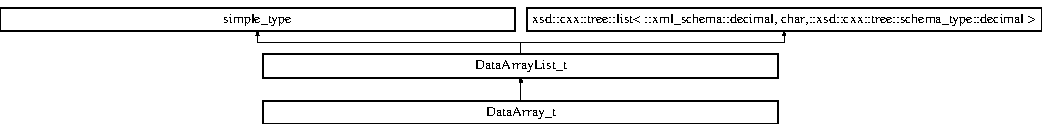
\includegraphics[height=1.660079cm]{classDataArrayList__t}
\end{center}
\end{figure}
\subsection*{Public Member Functions}
\begin{DoxyCompactItemize}
\item 
\hyperlink{classDataArrayList__t_a3ec10a5824450940e47a90c376fdb065}{Data\+Array\+List\+\_\+t} ()
\begin{DoxyCompactList}\small\item\em Default constructor. \end{DoxyCompactList}\item 
\hyperlink{classDataArrayList__t_ad821001ed5f5f94f06712f5b0acab874}{Data\+Array\+List\+\_\+t} (size\+\_\+type n, const \+::\hyperlink{namespacexml__schema_a69bfaf24f63a8c18ebd8e21db6b343df}{xml\+\_\+schema\+::decimal} \&x)
\begin{DoxyCompactList}\small\item\em Create a list with copies of the specified element. \end{DoxyCompactList}\item 
{\footnotesize template$<$typename I $>$ }\\\hyperlink{classDataArrayList__t_a7b3c40bcc5d41bafc235a30ffa1a3b8f}{Data\+Array\+List\+\_\+t} (const I \&begin, const I \&end)
\begin{DoxyCompactList}\small\item\em Create a list from an iterator range. \end{DoxyCompactList}\item 
\hyperlink{classDataArrayList__t_ab596ca97e9666c979d1db13a4e032869}{Data\+Array\+List\+\_\+t} (const \+::xercesc\+::\+D\+O\+M\+Element \&e,\+::\hyperlink{namespacexml__schema_a8d981c127a1f5106d04ad5853e707361}{xml\+\_\+schema\+::flags} f=0,\+::\hyperlink{namespacexml__schema_a395f5179c5fc4643909d66e9ff28d8ca}{xml\+\_\+schema\+::container} $\ast$c=0)
\begin{DoxyCompactList}\small\item\em Create an instance from a D\+O\+M element. \end{DoxyCompactList}\item 
\hyperlink{classDataArrayList__t_a4cae1891a3ad2b9336b478fa436f4d3f}{Data\+Array\+List\+\_\+t} (const \+::xercesc\+::\+D\+O\+M\+Attr \&a,\+::\hyperlink{namespacexml__schema_a8d981c127a1f5106d04ad5853e707361}{xml\+\_\+schema\+::flags} f=0,\+::\hyperlink{namespacexml__schema_a395f5179c5fc4643909d66e9ff28d8ca}{xml\+\_\+schema\+::container} $\ast$c=0)
\begin{DoxyCompactList}\small\item\em Create an instance from a D\+O\+M attribute. \end{DoxyCompactList}\item 
\hyperlink{classDataArrayList__t_a360a3281299fcb02ad34ad0b2c2d15fd}{Data\+Array\+List\+\_\+t} (const \+::std\+::string \&s, const \+::xercesc\+::\+D\+O\+M\+Element $\ast$e,\+::\hyperlink{namespacexml__schema_a8d981c127a1f5106d04ad5853e707361}{xml\+\_\+schema\+::flags} f=0,\+::\hyperlink{namespacexml__schema_a395f5179c5fc4643909d66e9ff28d8ca}{xml\+\_\+schema\+::container} $\ast$c=0)
\begin{DoxyCompactList}\small\item\em Create an instance from a string fragment. \end{DoxyCompactList}\item 
\hyperlink{classDataArrayList__t_af44b66e9ba5c6f84a3a0cca1c0fc98dc}{Data\+Array\+List\+\_\+t} (const \hyperlink{classDataArrayList__t}{Data\+Array\+List\+\_\+t} \&x,\+::\hyperlink{namespacexml__schema_a8d981c127a1f5106d04ad5853e707361}{xml\+\_\+schema\+::flags} f=0,\+::\hyperlink{namespacexml__schema_a395f5179c5fc4643909d66e9ff28d8ca}{xml\+\_\+schema\+::container} $\ast$c=0)
\begin{DoxyCompactList}\small\item\em Copy constructor. \end{DoxyCompactList}\item 
virtual \hyperlink{classDataArrayList__t}{Data\+Array\+List\+\_\+t} $\ast$ \hyperlink{classDataArrayList__t_acec29e88488ded1352c5b064827f5c38}{\+\_\+clone} (\+::\hyperlink{namespacexml__schema_a8d981c127a1f5106d04ad5853e707361}{xml\+\_\+schema\+::flags} f=0,\+::\hyperlink{namespacexml__schema_a395f5179c5fc4643909d66e9ff28d8ca}{xml\+\_\+schema\+::container} $\ast$c=0) const 
\begin{DoxyCompactList}\small\item\em Copy the instance polymorphically. \end{DoxyCompactList}\item 
virtual \hyperlink{classDataArrayList__t_aee3c16237122c72a9c163847232d830f}{$\sim$\+Data\+Array\+List\+\_\+t} ()
\begin{DoxyCompactList}\small\item\em Destructor. \end{DoxyCompactList}\end{DoxyCompactItemize}


\subsection{Detailed Description}
List class corresponding to the Data\+Array\+List\+\_\+t schema type. 

This class has an interface of a standard C++ sequence (e.\+g., std\+::vector). 

\subsection{Constructor \& Destructor Documentation}
\hypertarget{classDataArrayList__t_a3ec10a5824450940e47a90c376fdb065}{}\index{Data\+Array\+List\+\_\+t@{Data\+Array\+List\+\_\+t}!Data\+Array\+List\+\_\+t@{Data\+Array\+List\+\_\+t}}
\index{Data\+Array\+List\+\_\+t@{Data\+Array\+List\+\_\+t}!Data\+Array\+List\+\_\+t@{Data\+Array\+List\+\_\+t}}
\subsubsection[{Data\+Array\+List\+\_\+t}]{\setlength{\rightskip}{0pt plus 5cm}Data\+Array\+List\+\_\+t\+::\+Data\+Array\+List\+\_\+t (
\begin{DoxyParamCaption}
{}
\end{DoxyParamCaption}
)}\label{classDataArrayList__t_a3ec10a5824450940e47a90c376fdb065}


Default constructor. 

Creates an empty list. \hypertarget{classDataArrayList__t_ad821001ed5f5f94f06712f5b0acab874}{}\index{Data\+Array\+List\+\_\+t@{Data\+Array\+List\+\_\+t}!Data\+Array\+List\+\_\+t@{Data\+Array\+List\+\_\+t}}
\index{Data\+Array\+List\+\_\+t@{Data\+Array\+List\+\_\+t}!Data\+Array\+List\+\_\+t@{Data\+Array\+List\+\_\+t}}
\subsubsection[{Data\+Array\+List\+\_\+t}]{\setlength{\rightskip}{0pt plus 5cm}Data\+Array\+List\+\_\+t\+::\+Data\+Array\+List\+\_\+t (
\begin{DoxyParamCaption}
\item[{size\+\_\+type}]{n, }
\item[{const \+::{\bf xml\+\_\+schema\+::decimal} \&}]{x}
\end{DoxyParamCaption}
)}\label{classDataArrayList__t_ad821001ed5f5f94f06712f5b0acab874}


Create a list with copies of the specified element. 


\begin{DoxyParams}{Parameters}
{\em n} & A number of elements to copy. \\
\hline
{\em x} & An element to copy.\\
\hline
\end{DoxyParams}
This constructor creates a list with {\itshape n} copies of {\itshape x}. \hypertarget{classDataArrayList__t_a7b3c40bcc5d41bafc235a30ffa1a3b8f}{}\index{Data\+Array\+List\+\_\+t@{Data\+Array\+List\+\_\+t}!Data\+Array\+List\+\_\+t@{Data\+Array\+List\+\_\+t}}
\index{Data\+Array\+List\+\_\+t@{Data\+Array\+List\+\_\+t}!Data\+Array\+List\+\_\+t@{Data\+Array\+List\+\_\+t}}
\subsubsection[{Data\+Array\+List\+\_\+t}]{\setlength{\rightskip}{0pt plus 5cm}template$<$typename I $>$ Data\+Array\+List\+\_\+t\+::\+Data\+Array\+List\+\_\+t (
\begin{DoxyParamCaption}
\item[{const I \&}]{begin, }
\item[{const I \&}]{end}
\end{DoxyParamCaption}
)\hspace{0.3cm}{\ttfamily [inline]}}\label{classDataArrayList__t_a7b3c40bcc5d41bafc235a30ffa1a3b8f}


Create a list from an iterator range. 


\begin{DoxyParams}{Parameters}
{\em begin} & An iterator pointing to the first element. \\
\hline
{\em end} & An iterator pointing to the one past the last element.\\
\hline
\end{DoxyParams}
This constructor creates a list consisting of copies of the elements in the range \mbox{[}begin,end). \hypertarget{classDataArrayList__t_ab596ca97e9666c979d1db13a4e032869}{}\index{Data\+Array\+List\+\_\+t@{Data\+Array\+List\+\_\+t}!Data\+Array\+List\+\_\+t@{Data\+Array\+List\+\_\+t}}
\index{Data\+Array\+List\+\_\+t@{Data\+Array\+List\+\_\+t}!Data\+Array\+List\+\_\+t@{Data\+Array\+List\+\_\+t}}
\subsubsection[{Data\+Array\+List\+\_\+t}]{\setlength{\rightskip}{0pt plus 5cm}Data\+Array\+List\+\_\+t\+::\+Data\+Array\+List\+\_\+t (
\begin{DoxyParamCaption}
\item[{const \+::xercesc\+::\+D\+O\+M\+Element \&}]{e, }
\item[{\+::{\bf xml\+\_\+schema\+::flags}}]{f = {\ttfamily 0}, }
\item[{\+::{\bf xml\+\_\+schema\+::container} $\ast$}]{c = {\ttfamily 0}}
\end{DoxyParamCaption}
)}\label{classDataArrayList__t_ab596ca97e9666c979d1db13a4e032869}


Create an instance from a D\+O\+M element. 


\begin{DoxyParams}{Parameters}
{\em e} & A D\+O\+M element to extract the data from. \\
\hline
{\em f} & Flags to create the new instance with. \\
\hline
{\em c} & A pointer to the object that will contain the new instance. \\
\hline
\end{DoxyParams}
\hypertarget{classDataArrayList__t_a4cae1891a3ad2b9336b478fa436f4d3f}{}\index{Data\+Array\+List\+\_\+t@{Data\+Array\+List\+\_\+t}!Data\+Array\+List\+\_\+t@{Data\+Array\+List\+\_\+t}}
\index{Data\+Array\+List\+\_\+t@{Data\+Array\+List\+\_\+t}!Data\+Array\+List\+\_\+t@{Data\+Array\+List\+\_\+t}}
\subsubsection[{Data\+Array\+List\+\_\+t}]{\setlength{\rightskip}{0pt plus 5cm}Data\+Array\+List\+\_\+t\+::\+Data\+Array\+List\+\_\+t (
\begin{DoxyParamCaption}
\item[{const \+::xercesc\+::\+D\+O\+M\+Attr \&}]{a, }
\item[{\+::{\bf xml\+\_\+schema\+::flags}}]{f = {\ttfamily 0}, }
\item[{\+::{\bf xml\+\_\+schema\+::container} $\ast$}]{c = {\ttfamily 0}}
\end{DoxyParamCaption}
)}\label{classDataArrayList__t_a4cae1891a3ad2b9336b478fa436f4d3f}


Create an instance from a D\+O\+M attribute. 


\begin{DoxyParams}{Parameters}
{\em a} & A D\+O\+M attribute to extract the data from. \\
\hline
{\em f} & Flags to create the new instance with. \\
\hline
{\em c} & A pointer to the object that will contain the new instance. \\
\hline
\end{DoxyParams}
\hypertarget{classDataArrayList__t_a360a3281299fcb02ad34ad0b2c2d15fd}{}\index{Data\+Array\+List\+\_\+t@{Data\+Array\+List\+\_\+t}!Data\+Array\+List\+\_\+t@{Data\+Array\+List\+\_\+t}}
\index{Data\+Array\+List\+\_\+t@{Data\+Array\+List\+\_\+t}!Data\+Array\+List\+\_\+t@{Data\+Array\+List\+\_\+t}}
\subsubsection[{Data\+Array\+List\+\_\+t}]{\setlength{\rightskip}{0pt plus 5cm}Data\+Array\+List\+\_\+t\+::\+Data\+Array\+List\+\_\+t (
\begin{DoxyParamCaption}
\item[{const \+::std\+::string \&}]{s, }
\item[{const \+::xercesc\+::\+D\+O\+M\+Element $\ast$}]{e, }
\item[{\+::{\bf xml\+\_\+schema\+::flags}}]{f = {\ttfamily 0}, }
\item[{\+::{\bf xml\+\_\+schema\+::container} $\ast$}]{c = {\ttfamily 0}}
\end{DoxyParamCaption}
)}\label{classDataArrayList__t_a360a3281299fcb02ad34ad0b2c2d15fd}


Create an instance from a string fragment. 


\begin{DoxyParams}{Parameters}
{\em s} & A string fragment to extract the data from. \\
\hline
{\em e} & A pointer to D\+O\+M element containing the string fragment. \\
\hline
{\em f} & Flags to create the new instance with. \\
\hline
{\em c} & A pointer to the object that will contain the new instance. \\
\hline
\end{DoxyParams}
\hypertarget{classDataArrayList__t_af44b66e9ba5c6f84a3a0cca1c0fc98dc}{}\index{Data\+Array\+List\+\_\+t@{Data\+Array\+List\+\_\+t}!Data\+Array\+List\+\_\+t@{Data\+Array\+List\+\_\+t}}
\index{Data\+Array\+List\+\_\+t@{Data\+Array\+List\+\_\+t}!Data\+Array\+List\+\_\+t@{Data\+Array\+List\+\_\+t}}
\subsubsection[{Data\+Array\+List\+\_\+t}]{\setlength{\rightskip}{0pt plus 5cm}Data\+Array\+List\+\_\+t\+::\+Data\+Array\+List\+\_\+t (
\begin{DoxyParamCaption}
\item[{const {\bf Data\+Array\+List\+\_\+t} \&}]{x, }
\item[{\+::{\bf xml\+\_\+schema\+::flags}}]{f = {\ttfamily 0}, }
\item[{\+::{\bf xml\+\_\+schema\+::container} $\ast$}]{c = {\ttfamily 0}}
\end{DoxyParamCaption}
)}\label{classDataArrayList__t_af44b66e9ba5c6f84a3a0cca1c0fc98dc}


Copy constructor. 


\begin{DoxyParams}{Parameters}
{\em x} & An instance to make a copy of. \\
\hline
{\em f} & Flags to create the copy with. \\
\hline
{\em c} & A pointer to the object that will contain the copy.\\
\hline
\end{DoxyParams}
For polymorphic object models use the {\ttfamily \+\_\+clone} function instead. \hypertarget{classDataArrayList__t_aee3c16237122c72a9c163847232d830f}{}\index{Data\+Array\+List\+\_\+t@{Data\+Array\+List\+\_\+t}!````~Data\+Array\+List\+\_\+t@{$\sim$\+Data\+Array\+List\+\_\+t}}
\index{````~Data\+Array\+List\+\_\+t@{$\sim$\+Data\+Array\+List\+\_\+t}!Data\+Array\+List\+\_\+t@{Data\+Array\+List\+\_\+t}}
\subsubsection[{$\sim$\+Data\+Array\+List\+\_\+t}]{\setlength{\rightskip}{0pt plus 5cm}Data\+Array\+List\+\_\+t\+::$\sim$\+Data\+Array\+List\+\_\+t (
\begin{DoxyParamCaption}
{}
\end{DoxyParamCaption}
)\hspace{0.3cm}{\ttfamily [virtual]}}\label{classDataArrayList__t_aee3c16237122c72a9c163847232d830f}


Destructor. 



\subsection{Member Function Documentation}
\hypertarget{classDataArrayList__t_acec29e88488ded1352c5b064827f5c38}{}\index{Data\+Array\+List\+\_\+t@{Data\+Array\+List\+\_\+t}!\+\_\+clone@{\+\_\+clone}}
\index{\+\_\+clone@{\+\_\+clone}!Data\+Array\+List\+\_\+t@{Data\+Array\+List\+\_\+t}}
\subsubsection[{\+\_\+clone}]{\setlength{\rightskip}{0pt plus 5cm}{\bf Data\+Array\+List\+\_\+t} $\ast$ Data\+Array\+List\+\_\+t\+::\+\_\+clone (
\begin{DoxyParamCaption}
\item[{\+::{\bf xml\+\_\+schema\+::flags}}]{f = {\ttfamily 0}, }
\item[{\+::{\bf xml\+\_\+schema\+::container} $\ast$}]{c = {\ttfamily 0}}
\end{DoxyParamCaption}
) const\hspace{0.3cm}{\ttfamily [virtual]}}\label{classDataArrayList__t_acec29e88488ded1352c5b064827f5c38}


Copy the instance polymorphically. 


\begin{DoxyParams}{Parameters}
{\em f} & Flags to create the copy with. \\
\hline
{\em c} & A pointer to the object that will contain the copy. \\
\hline
\end{DoxyParams}
\begin{DoxyReturn}{Returns}
A pointer to the dynamically allocated copy.
\end{DoxyReturn}
This function ensures that the dynamic type of the instance is used for copying and should be used for polymorphic object models instead of the copy constructor. 

Reimplemented in \hyperlink{classDataArray__t_a0ba3569846912b9fcadbd942e914cce1}{Data\+Array\+\_\+t}.



The documentation for this class was generated from the following files\+:\begin{DoxyCompactItemize}
\item 
src/output\+Writer/\hyperlink{vtk-unstructured_8h}{vtk-\/unstructured.\+h}\item 
src/output\+Writer/\hyperlink{vtk-unstructured_8cpp}{vtk-\/unstructured.\+cpp}\end{DoxyCompactItemize}

\hypertarget{classFileReader}{}\section{File\+Reader Class Reference}
\label{classFileReader}\index{File\+Reader@{File\+Reader}}


{\ttfamily \#include $<$File\+Reader.\+h$>$}

\subsection*{Public Member Functions}
\begin{DoxyCompactItemize}
\item 
\hyperlink{classFileReader_a615dcb2443cad1f2ca123c7c0c334480}{File\+Reader} ()
\item 
virtual \hyperlink{classFileReader_a1382969e8f1468f3b04ad4b44ab39dee}{$\sim$\+File\+Reader} ()
\item 
void \hyperlink{classFileReader_a64f3f751b42d2c7f04e4114076aa7e81}{read\+File} (\hyperlink{classParticleContainer}{Particle\+Container} \&\hyperlink{MolSim_8cpp_a6b352757b6951d85f71bd9cbc47cf619}{particles}, char $\ast$filename)
\end{DoxyCompactItemize}


\subsection{Constructor \& Destructor Documentation}
\hypertarget{classFileReader_a615dcb2443cad1f2ca123c7c0c334480}{}\index{File\+Reader@{File\+Reader}!File\+Reader@{File\+Reader}}
\index{File\+Reader@{File\+Reader}!File\+Reader@{File\+Reader}}
\subsubsection[{File\+Reader}]{\setlength{\rightskip}{0pt plus 5cm}File\+Reader\+::\+File\+Reader (
\begin{DoxyParamCaption}
{}
\end{DoxyParamCaption}
)}\label{classFileReader_a615dcb2443cad1f2ca123c7c0c334480}
\hypertarget{classFileReader_a1382969e8f1468f3b04ad4b44ab39dee}{}\index{File\+Reader@{File\+Reader}!````~File\+Reader@{$\sim$\+File\+Reader}}
\index{````~File\+Reader@{$\sim$\+File\+Reader}!File\+Reader@{File\+Reader}}
\subsubsection[{$\sim$\+File\+Reader}]{\setlength{\rightskip}{0pt plus 5cm}File\+Reader\+::$\sim$\+File\+Reader (
\begin{DoxyParamCaption}
{}
\end{DoxyParamCaption}
)\hspace{0.3cm}{\ttfamily [virtual]}}\label{classFileReader_a1382969e8f1468f3b04ad4b44ab39dee}


\subsection{Member Function Documentation}
\hypertarget{classFileReader_a64f3f751b42d2c7f04e4114076aa7e81}{}\index{File\+Reader@{File\+Reader}!read\+File@{read\+File}}
\index{read\+File@{read\+File}!File\+Reader@{File\+Reader}}
\subsubsection[{read\+File}]{\setlength{\rightskip}{0pt plus 5cm}void File\+Reader\+::read\+File (
\begin{DoxyParamCaption}
\item[{{\bf Particle\+Container} \&}]{particles, }
\item[{char $\ast$}]{filename}
\end{DoxyParamCaption}
)}\label{classFileReader_a64f3f751b42d2c7f04e4114076aa7e81}


The documentation for this class was generated from the following files\+:\begin{DoxyCompactItemize}
\item 
src/\hyperlink{FileReader_8h}{File\+Reader.\+h}\item 
src/\hyperlink{FileReader_8cpp}{File\+Reader.\+cpp}\end{DoxyCompactItemize}

\hypertarget{classParticle}{}\section{Particle Class Reference}
\label{classParticle}\index{Particle@{Particle}}


{\ttfamily \#include $<$Particle.\+h$>$}

\subsection*{Public Member Functions}
\begin{DoxyCompactItemize}
\item 
\hyperlink{classParticle_a866812d3dfb9c539e5e24593e596a8c9}{Particle} (int \hyperlink{classtype}{type}=0)
\item 
\hyperlink{classParticle_a24b04cb7c6f7ea4242d25c410f44ae56}{Particle} (const \hyperlink{classParticle}{Particle} \&other)
\item 
\hyperlink{classParticle_a5a5b07aa732c302b45e90c12723f2b27}{Particle} (\hyperlink{classutils_1_1Vector}{utils\+::\+Vector}$<$ double, 3 $>$ x\+\_\+arg, \hyperlink{classutils_1_1Vector}{utils\+::\+Vector}$<$ double, 3 $>$ v\+\_\+arg, double m\+\_\+arg, int \hyperlink{classtype}{type}=0)
\item 
virtual \hyperlink{classParticle_ad030d0fe7b88cf81744b127c99244ff4}{$\sim$\+Particle} ()
\item 
\hyperlink{classutils_1_1Vector}{utils\+::\+Vector}$<$ double, 3 $>$ \& \hyperlink{classParticle_ab7ade5dc156dfa0234aa0323564e46ed}{get\+X} ()
\item 
\hyperlink{classutils_1_1Vector}{utils\+::\+Vector}$<$ double, 3 $>$ \& \hyperlink{classParticle_acd84c445e2bd5f5280a00e76cfe73fe0}{get\+F} ()
\item 
\hyperlink{classutils_1_1Vector}{utils\+::\+Vector}$<$ double, 3 $>$ \& \hyperlink{classParticle_a1204435fc08c697b0fea230616d1bbdf}{get\+Old\+F} ()
\item 
\hyperlink{classutils_1_1Vector}{utils\+::\+Vector}$<$ double, 3 $>$ \& \hyperlink{classParticle_aaf3ecbc6e1e31b259fe239461ba13dbd}{get\+V} ()
\item 
double \hyperlink{classParticle_aa1ca800f9be9dd4bd6c604f608095b24}{get\+M} ()
\item 
int \hyperlink{classParticle_a0581d7b629eb17ac5bef8e934852ca8b}{get\+Type} ()
\item 
bool \hyperlink{classParticle_a5034babb77618a56e00927d8891afabe}{operator==} (\hyperlink{classParticle}{Particle} \&other)
\item 
std\+::string \hyperlink{classParticle_a07d071a0f91f8ce7413201a6db3afe7b}{to\+String} ()
\end{DoxyCompactItemize}
\subsection*{Private Attributes}
\begin{DoxyCompactItemize}
\item 
\hyperlink{classutils_1_1Vector}{utils\+::\+Vector}$<$ double, 3 $>$ \hyperlink{classParticle_a3789900d6fe19a75d3a82cd5e9622c4c}{x}
\item 
\hyperlink{classutils_1_1Vector}{utils\+::\+Vector}$<$ double, 3 $>$ \hyperlink{classParticle_ac3669e50d83d8608d522965b9acd1d8b}{v}
\item 
\hyperlink{classutils_1_1Vector}{utils\+::\+Vector}$<$ double, 3 $>$ \hyperlink{classParticle_ad9aa3e171ea950b2cff1b4825e67845b}{f}
\item 
\hyperlink{classutils_1_1Vector}{utils\+::\+Vector}$<$ double, 3 $>$ \hyperlink{classParticle_ad9281e33474f23f7261f28848affc4a4}{old\+\_\+f}
\item 
double \hyperlink{classParticle_aedcc7e1bc53b0e2b1a4a07c9a1b47563}{m}
\item 
int \hyperlink{classParticle_a2b73dd42bcd56ba2e7ffeb0a5515a866}{type}
\end{DoxyCompactItemize}


\subsection{Constructor \& Destructor Documentation}
\hypertarget{classParticle_a866812d3dfb9c539e5e24593e596a8c9}{}\index{Particle@{Particle}!Particle@{Particle}}
\index{Particle@{Particle}!Particle@{Particle}}
\subsubsection[{Particle}]{\setlength{\rightskip}{0pt plus 5cm}Particle\+::\+Particle (
\begin{DoxyParamCaption}
\item[{int}]{type = {\ttfamily 0}}
\end{DoxyParamCaption}
)}\label{classParticle_a866812d3dfb9c539e5e24593e596a8c9}
\hypertarget{classParticle_a24b04cb7c6f7ea4242d25c410f44ae56}{}\index{Particle@{Particle}!Particle@{Particle}}
\index{Particle@{Particle}!Particle@{Particle}}
\subsubsection[{Particle}]{\setlength{\rightskip}{0pt plus 5cm}Particle\+::\+Particle (
\begin{DoxyParamCaption}
\item[{const {\bf Particle} \&}]{other}
\end{DoxyParamCaption}
)}\label{classParticle_a24b04cb7c6f7ea4242d25c410f44ae56}
\hypertarget{classParticle_a5a5b07aa732c302b45e90c12723f2b27}{}\index{Particle@{Particle}!Particle@{Particle}}
\index{Particle@{Particle}!Particle@{Particle}}
\subsubsection[{Particle}]{\setlength{\rightskip}{0pt plus 5cm}Particle\+::\+Particle (
\begin{DoxyParamCaption}
\item[{{\bf utils\+::\+Vector}$<$ double, 3 $>$}]{x\+\_\+arg, }
\item[{{\bf utils\+::\+Vector}$<$ double, 3 $>$}]{v\+\_\+arg, }
\item[{double}]{m\+\_\+arg, }
\item[{int}]{type = {\ttfamily 0}}
\end{DoxyParamCaption}
)}\label{classParticle_a5a5b07aa732c302b45e90c12723f2b27}
\hypertarget{classParticle_ad030d0fe7b88cf81744b127c99244ff4}{}\index{Particle@{Particle}!````~Particle@{$\sim$\+Particle}}
\index{````~Particle@{$\sim$\+Particle}!Particle@{Particle}}
\subsubsection[{$\sim$\+Particle}]{\setlength{\rightskip}{0pt plus 5cm}Particle\+::$\sim$\+Particle (
\begin{DoxyParamCaption}
{}
\end{DoxyParamCaption}
)\hspace{0.3cm}{\ttfamily [virtual]}}\label{classParticle_ad030d0fe7b88cf81744b127c99244ff4}


\subsection{Member Function Documentation}
\hypertarget{classParticle_acd84c445e2bd5f5280a00e76cfe73fe0}{}\index{Particle@{Particle}!get\+F@{get\+F}}
\index{get\+F@{get\+F}!Particle@{Particle}}
\subsubsection[{get\+F}]{\setlength{\rightskip}{0pt plus 5cm}{\bf utils\+::\+Vector}$<$ double, 3 $>$ \& Particle\+::get\+F (
\begin{DoxyParamCaption}
{}
\end{DoxyParamCaption}
)}\label{classParticle_acd84c445e2bd5f5280a00e76cfe73fe0}
\hypertarget{classParticle_aa1ca800f9be9dd4bd6c604f608095b24}{}\index{Particle@{Particle}!get\+M@{get\+M}}
\index{get\+M@{get\+M}!Particle@{Particle}}
\subsubsection[{get\+M}]{\setlength{\rightskip}{0pt plus 5cm}double Particle\+::get\+M (
\begin{DoxyParamCaption}
{}
\end{DoxyParamCaption}
)}\label{classParticle_aa1ca800f9be9dd4bd6c604f608095b24}
\hypertarget{classParticle_a1204435fc08c697b0fea230616d1bbdf}{}\index{Particle@{Particle}!get\+Old\+F@{get\+Old\+F}}
\index{get\+Old\+F@{get\+Old\+F}!Particle@{Particle}}
\subsubsection[{get\+Old\+F}]{\setlength{\rightskip}{0pt plus 5cm}{\bf utils\+::\+Vector}$<$ double, 3 $>$ \& Particle\+::get\+Old\+F (
\begin{DoxyParamCaption}
{}
\end{DoxyParamCaption}
)}\label{classParticle_a1204435fc08c697b0fea230616d1bbdf}
\hypertarget{classParticle_a0581d7b629eb17ac5bef8e934852ca8b}{}\index{Particle@{Particle}!get\+Type@{get\+Type}}
\index{get\+Type@{get\+Type}!Particle@{Particle}}
\subsubsection[{get\+Type}]{\setlength{\rightskip}{0pt plus 5cm}int Particle\+::get\+Type (
\begin{DoxyParamCaption}
{}
\end{DoxyParamCaption}
)}\label{classParticle_a0581d7b629eb17ac5bef8e934852ca8b}
\hypertarget{classParticle_aaf3ecbc6e1e31b259fe239461ba13dbd}{}\index{Particle@{Particle}!get\+V@{get\+V}}
\index{get\+V@{get\+V}!Particle@{Particle}}
\subsubsection[{get\+V}]{\setlength{\rightskip}{0pt plus 5cm}{\bf utils\+::\+Vector}$<$ double, 3 $>$ \& Particle\+::get\+V (
\begin{DoxyParamCaption}
{}
\end{DoxyParamCaption}
)}\label{classParticle_aaf3ecbc6e1e31b259fe239461ba13dbd}
\hypertarget{classParticle_ab7ade5dc156dfa0234aa0323564e46ed}{}\index{Particle@{Particle}!get\+X@{get\+X}}
\index{get\+X@{get\+X}!Particle@{Particle}}
\subsubsection[{get\+X}]{\setlength{\rightskip}{0pt plus 5cm}{\bf utils\+::\+Vector}$<$ double, 3 $>$ \& Particle\+::get\+X (
\begin{DoxyParamCaption}
{}
\end{DoxyParamCaption}
)}\label{classParticle_ab7ade5dc156dfa0234aa0323564e46ed}
\hypertarget{classParticle_a5034babb77618a56e00927d8891afabe}{}\index{Particle@{Particle}!operator==@{operator==}}
\index{operator==@{operator==}!Particle@{Particle}}
\subsubsection[{operator==}]{\setlength{\rightskip}{0pt plus 5cm}bool Particle\+::operator== (
\begin{DoxyParamCaption}
\item[{{\bf Particle} \&}]{other}
\end{DoxyParamCaption}
)}\label{classParticle_a5034babb77618a56e00927d8891afabe}
\hypertarget{classParticle_a07d071a0f91f8ce7413201a6db3afe7b}{}\index{Particle@{Particle}!to\+String@{to\+String}}
\index{to\+String@{to\+String}!Particle@{Particle}}
\subsubsection[{to\+String}]{\setlength{\rightskip}{0pt plus 5cm}std\+::string Particle\+::to\+String (
\begin{DoxyParamCaption}
{}
\end{DoxyParamCaption}
)}\label{classParticle_a07d071a0f91f8ce7413201a6db3afe7b}


\subsection{Member Data Documentation}
\hypertarget{classParticle_ad9aa3e171ea950b2cff1b4825e67845b}{}\index{Particle@{Particle}!f@{f}}
\index{f@{f}!Particle@{Particle}}
\subsubsection[{f}]{\setlength{\rightskip}{0pt plus 5cm}{\bf utils\+::\+Vector}$<$double, 3$>$ Particle\+::f\hspace{0.3cm}{\ttfamily [private]}}\label{classParticle_ad9aa3e171ea950b2cff1b4825e67845b}
the force effective on this particle \hypertarget{classParticle_aedcc7e1bc53b0e2b1a4a07c9a1b47563}{}\index{Particle@{Particle}!m@{m}}
\index{m@{m}!Particle@{Particle}}
\subsubsection[{m}]{\setlength{\rightskip}{0pt plus 5cm}double Particle\+::m\hspace{0.3cm}{\ttfamily [private]}}\label{classParticle_aedcc7e1bc53b0e2b1a4a07c9a1b47563}
the mass of this particle \hypertarget{classParticle_ad9281e33474f23f7261f28848affc4a4}{}\index{Particle@{Particle}!old\+\_\+f@{old\+\_\+f}}
\index{old\+\_\+f@{old\+\_\+f}!Particle@{Particle}}
\subsubsection[{old\+\_\+f}]{\setlength{\rightskip}{0pt plus 5cm}{\bf utils\+::\+Vector}$<$double, 3$>$ Particle\+::old\+\_\+f\hspace{0.3cm}{\ttfamily [private]}}\label{classParticle_ad9281e33474f23f7261f28848affc4a4}
the force which was effective on this particle \hypertarget{classParticle_a2b73dd42bcd56ba2e7ffeb0a5515a866}{}\index{Particle@{Particle}!type@{type}}
\index{type@{type}!Particle@{Particle}}
\subsubsection[{type}]{\setlength{\rightskip}{0pt plus 5cm}int Particle\+::type\hspace{0.3cm}{\ttfamily [private]}}\label{classParticle_a2b73dd42bcd56ba2e7ffeb0a5515a866}
type of the particle. Use it for whatever you want (e.\+g. to seperate molecules belonging to different bodies, matters, and so on) \hypertarget{classParticle_ac3669e50d83d8608d522965b9acd1d8b}{}\index{Particle@{Particle}!v@{v}}
\index{v@{v}!Particle@{Particle}}
\subsubsection[{v}]{\setlength{\rightskip}{0pt plus 5cm}{\bf utils\+::\+Vector}$<$double, 3$>$ Particle\+::v\hspace{0.3cm}{\ttfamily [private]}}\label{classParticle_ac3669e50d83d8608d522965b9acd1d8b}
the velocity of the particle \hypertarget{classParticle_a3789900d6fe19a75d3a82cd5e9622c4c}{}\index{Particle@{Particle}!x@{x}}
\index{x@{x}!Particle@{Particle}}
\subsubsection[{x}]{\setlength{\rightskip}{0pt plus 5cm}{\bf utils\+::\+Vector}$<$double, 3$>$ Particle\+::x\hspace{0.3cm}{\ttfamily [private]}}\label{classParticle_a3789900d6fe19a75d3a82cd5e9622c4c}
the position of the particle 

The documentation for this class was generated from the following files\+:\begin{DoxyCompactItemize}
\item 
src/\hyperlink{Particle_8h}{Particle.\+h}\item 
src/\hyperlink{Particle_8cpp}{Particle.\+cpp}\end{DoxyCompactItemize}

\hypertarget{classParticleContainer}{}\section{Particle\+Container Class Reference}
\label{classParticleContainer}\index{Particle\+Container@{Particle\+Container}}


{\ttfamily \#include $<$Particle\+Container.\+h$>$}

\subsection*{Public Member Functions}
\begin{DoxyCompactItemize}
\item 
\hyperlink{classParticleContainer_a76d21bdb5141158cf664d65e2d8b1db7}{Particle\+Container} ()
\item 
\hyperlink{classParticleContainer_a3bd4be6aa403538ae5ad2486aa00573c}{Particle\+Container} (int n)
\item 
\hyperlink{classParticleContainer_a2141e6ca39db88b9571ea353226cf9be}{Particle\+Container} (const \hyperlink{classParticleContainer}{Particle\+Container} \&pc)
\item 
\hyperlink{classParticleContainer_af5a354c93415a3dad049cb3d1e36ea68}{Particle\+Container} (const vector$<$ \hyperlink{classParticle}{Particle} $>$ pvector)
\item 
void \hyperlink{classParticleContainer_a39d2ad5e9c6aff35fc5b41586e6b38b5}{add} (const \hyperlink{classParticle}{Particle} \&p)
\item 
size\+\_\+t \hyperlink{classParticleContainer_a1c9372075d296dc6409c21c4dcab6fb1}{size} ()
\item 
\hyperlink{classParticle}{Particle} \& \hyperlink{classParticleContainer_aeb7ed6e001bf1db025e688463e497fe7}{operator\mbox{[}$\,$\mbox{]}} (size\+\_\+t i)
\item 
vector$<$ \hyperlink{classParticle}{Particle} $>$\+::iterator \hyperlink{classParticleContainer_adb4830a518ab84b106e8b822f1daa884}{begin} ()
\item 
vector$<$ \hyperlink{classParticle}{Particle} $>$\+::iterator \hyperlink{classParticleContainer_ab2e17cea64b42fb049848fa6f7c56c81}{end} ()
\end{DoxyCompactItemize}
\subsection*{Private Attributes}
\begin{DoxyCompactItemize}
\item 
vector$<$ \hyperlink{classParticle}{Particle} $>$ \hyperlink{classParticleContainer_a7bc512a3ee04b6bae0d22f61097f4e8c}{particles}
\end{DoxyCompactItemize}


\subsection{Constructor \& Destructor Documentation}
\hypertarget{classParticleContainer_a76d21bdb5141158cf664d65e2d8b1db7}{}\index{Particle\+Container@{Particle\+Container}!Particle\+Container@{Particle\+Container}}
\index{Particle\+Container@{Particle\+Container}!Particle\+Container@{Particle\+Container}}
\subsubsection[{Particle\+Container}]{\setlength{\rightskip}{0pt plus 5cm}Particle\+Container\+::\+Particle\+Container (
\begin{DoxyParamCaption}
{}
\end{DoxyParamCaption}
)}\label{classParticleContainer_a76d21bdb5141158cf664d65e2d8b1db7}
Creates an empty container \hypertarget{classParticleContainer_a3bd4be6aa403538ae5ad2486aa00573c}{}\index{Particle\+Container@{Particle\+Container}!Particle\+Container@{Particle\+Container}}
\index{Particle\+Container@{Particle\+Container}!Particle\+Container@{Particle\+Container}}
\subsubsection[{Particle\+Container}]{\setlength{\rightskip}{0pt plus 5cm}Particle\+Container\+::\+Particle\+Container (
\begin{DoxyParamCaption}
\item[{int}]{n}
\end{DoxyParamCaption}
)}\label{classParticleContainer_a3bd4be6aa403538ae5ad2486aa00573c}
Creates a container with n elements \hypertarget{classParticleContainer_a2141e6ca39db88b9571ea353226cf9be}{}\index{Particle\+Container@{Particle\+Container}!Particle\+Container@{Particle\+Container}}
\index{Particle\+Container@{Particle\+Container}!Particle\+Container@{Particle\+Container}}
\subsubsection[{Particle\+Container}]{\setlength{\rightskip}{0pt plus 5cm}Particle\+Container\+::\+Particle\+Container (
\begin{DoxyParamCaption}
\item[{const {\bf Particle\+Container} \&}]{pc}
\end{DoxyParamCaption}
)}\label{classParticleContainer_a2141e6ca39db88b9571ea353226cf9be}
Creates a copy of the passed container \hypertarget{classParticleContainer_af5a354c93415a3dad049cb3d1e36ea68}{}\index{Particle\+Container@{Particle\+Container}!Particle\+Container@{Particle\+Container}}
\index{Particle\+Container@{Particle\+Container}!Particle\+Container@{Particle\+Container}}
\subsubsection[{Particle\+Container}]{\setlength{\rightskip}{0pt plus 5cm}Particle\+Container\+::\+Particle\+Container (
\begin{DoxyParamCaption}
\item[{const vector$<$ {\bf Particle} $>$}]{pvector}
\end{DoxyParamCaption}
)}\label{classParticleContainer_af5a354c93415a3dad049cb3d1e36ea68}
Creates a \hyperlink{classParticleContainer}{Particle\+Container} of the passed list 

\subsection{Member Function Documentation}
\hypertarget{classParticleContainer_a39d2ad5e9c6aff35fc5b41586e6b38b5}{}\index{Particle\+Container@{Particle\+Container}!add@{add}}
\index{add@{add}!Particle\+Container@{Particle\+Container}}
\subsubsection[{add}]{\setlength{\rightskip}{0pt plus 5cm}void Particle\+Container\+::add (
\begin{DoxyParamCaption}
\item[{const {\bf Particle} \&}]{p}
\end{DoxyParamCaption}
)}\label{classParticleContainer_a39d2ad5e9c6aff35fc5b41586e6b38b5}
Adds an element to the container \hypertarget{classParticleContainer_adb4830a518ab84b106e8b822f1daa884}{}\index{Particle\+Container@{Particle\+Container}!begin@{begin}}
\index{begin@{begin}!Particle\+Container@{Particle\+Container}}
\subsubsection[{begin}]{\setlength{\rightskip}{0pt plus 5cm}vector$<$ {\bf Particle} $>$\+::iterator Particle\+Container\+::begin (
\begin{DoxyParamCaption}
{}
\end{DoxyParamCaption}
)}\label{classParticleContainer_adb4830a518ab84b106e8b822f1daa884}
Returns an iterator to the beginning of the container \hypertarget{classParticleContainer_ab2e17cea64b42fb049848fa6f7c56c81}{}\index{Particle\+Container@{Particle\+Container}!end@{end}}
\index{end@{end}!Particle\+Container@{Particle\+Container}}
\subsubsection[{end}]{\setlength{\rightskip}{0pt plus 5cm}vector$<$ {\bf Particle} $>$\+::iterator Particle\+Container\+::end (
\begin{DoxyParamCaption}
{}
\end{DoxyParamCaption}
)}\label{classParticleContainer_ab2e17cea64b42fb049848fa6f7c56c81}
Returns an iterator to the next element after the end of the container \hypertarget{classParticleContainer_aeb7ed6e001bf1db025e688463e497fe7}{}\index{Particle\+Container@{Particle\+Container}!operator\mbox{[}$\,$\mbox{]}@{operator[]}}
\index{operator\mbox{[}$\,$\mbox{]}@{operator[]}!Particle\+Container@{Particle\+Container}}
\subsubsection[{operator[]}]{\setlength{\rightskip}{0pt plus 5cm}{\bf Particle} \& Particle\+Container\+::operator\mbox{[}$\,$\mbox{]} (
\begin{DoxyParamCaption}
\item[{size\+\_\+t}]{i}
\end{DoxyParamCaption}
)}\label{classParticleContainer_aeb7ed6e001bf1db025e688463e497fe7}
Returns a pointer to the i-\/th element \hypertarget{classParticleContainer_a1c9372075d296dc6409c21c4dcab6fb1}{}\index{Particle\+Container@{Particle\+Container}!size@{size}}
\index{size@{size}!Particle\+Container@{Particle\+Container}}
\subsubsection[{size}]{\setlength{\rightskip}{0pt plus 5cm}size\+\_\+t Particle\+Container\+::size (
\begin{DoxyParamCaption}
{}
\end{DoxyParamCaption}
)}\label{classParticleContainer_a1c9372075d296dc6409c21c4dcab6fb1}
Returns the number of elements in the container 

\subsection{Member Data Documentation}
\hypertarget{classParticleContainer_a7bc512a3ee04b6bae0d22f61097f4e8c}{}\index{Particle\+Container@{Particle\+Container}!particles@{particles}}
\index{particles@{particles}!Particle\+Container@{Particle\+Container}}
\subsubsection[{particles}]{\setlength{\rightskip}{0pt plus 5cm}vector$<${\bf Particle}$>$ Particle\+Container\+::particles\hspace{0.3cm}{\ttfamily [private]}}\label{classParticleContainer_a7bc512a3ee04b6bae0d22f61097f4e8c}


The documentation for this class was generated from the following files\+:\begin{DoxyCompactItemize}
\item 
src/\hyperlink{ParticleContainer_8h}{Particle\+Container.\+h}\item 
src/\hyperlink{ParticleContainer_8cpp}{Particle\+Container.\+cpp}\end{DoxyCompactItemize}

\hypertarget{classPieceUnstructuredGrid__t}{}\section{Piece\+Unstructured\+Grid\+\_\+t Class Reference}
\label{classPieceUnstructuredGrid__t}\index{Piece\+Unstructured\+Grid\+\_\+t@{Piece\+Unstructured\+Grid\+\_\+t}}


Class corresponding to the Piece\+Unstructured\+Grid\+\_\+t schema type.  




{\ttfamily \#include $<$vtk-\/unstructured.\+h$>$}

Inheritance diagram for Piece\+Unstructured\+Grid\+\_\+t\+:\begin{figure}[H]
\begin{center}
\leavevmode
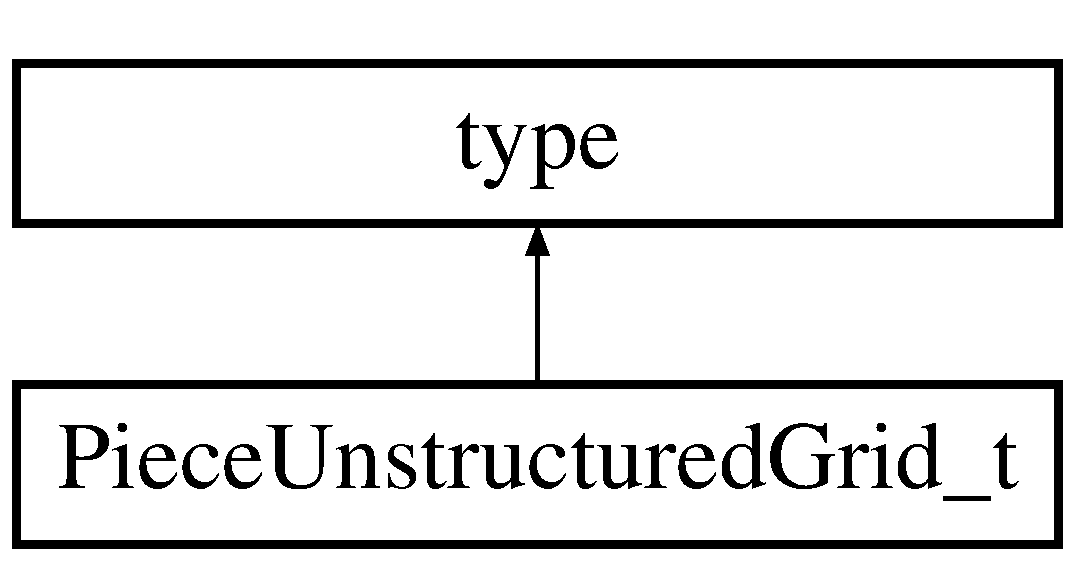
\includegraphics[height=2.000000cm]{classPieceUnstructuredGrid__t}
\end{center}
\end{figure}
\subsection*{Public Member Functions}
\begin{DoxyCompactItemize}
\item 
virtual \hyperlink{classPieceUnstructuredGrid__t_a9d1eb720775ac4e3b7778f898decc264}{$\sim$\+Piece\+Unstructured\+Grid\+\_\+t} ()
\begin{DoxyCompactList}\small\item\em Destructor. \end{DoxyCompactList}\end{DoxyCompactItemize}
\subsection*{Point\+Data}
\label{_amgrpe540450fb956cd9dbb96f979e5939d0f}%
Accessor and modifier functions for the Point\+Data required element. \begin{DoxyCompactItemize}
\item 
typedef \+::\hyperlink{classPointData}{Point\+Data} \hyperlink{classPieceUnstructuredGrid__t_a5d79d8ea03ca53f80f24e62c2175ec02}{Point\+Data\+\_\+type}
\begin{DoxyCompactList}\small\item\em Element type. \end{DoxyCompactList}\item 
typedef \+::xsd\+::cxx\+::tree\+::traits$<$ \hyperlink{classPieceUnstructuredGrid__t_a5d79d8ea03ca53f80f24e62c2175ec02}{Point\+Data\+\_\+type}, char $>$ \hyperlink{classPieceUnstructuredGrid__t_aee3c7ac7c46c4ebc9f248d31c458d300}{Point\+Data\+\_\+traits}
\begin{DoxyCompactList}\small\item\em Element traits type. \end{DoxyCompactList}\item 
const \hyperlink{classPieceUnstructuredGrid__t_a5d79d8ea03ca53f80f24e62c2175ec02}{Point\+Data\+\_\+type} \& \hyperlink{classPieceUnstructuredGrid__t_a4825627cfe05949b680c81826e9d4ea5}{Point\+Data} () const 
\begin{DoxyCompactList}\small\item\em Return a read-\/only (constant) reference to the element. \end{DoxyCompactList}\item 
\hyperlink{classPieceUnstructuredGrid__t_a5d79d8ea03ca53f80f24e62c2175ec02}{Point\+Data\+\_\+type} \& \hyperlink{classPieceUnstructuredGrid__t_af3a9955626dac2aad17bf879a77d2c0d}{Point\+Data} ()
\begin{DoxyCompactList}\small\item\em Return a read-\/write reference to the element. \end{DoxyCompactList}\item 
void \hyperlink{classPieceUnstructuredGrid__t_aee7745ad1ce39af5fc048e50acb76424}{Point\+Data} (const \hyperlink{classPieceUnstructuredGrid__t_a5d79d8ea03ca53f80f24e62c2175ec02}{Point\+Data\+\_\+type} \&x)
\begin{DoxyCompactList}\small\item\em Set the element value. \end{DoxyCompactList}\item 
void \hyperlink{classPieceUnstructuredGrid__t_a752f5abf0faba70deaab0b4990677612}{Point\+Data} (\+::std\+::auto\+\_\+ptr$<$ \hyperlink{classPieceUnstructuredGrid__t_a5d79d8ea03ca53f80f24e62c2175ec02}{Point\+Data\+\_\+type} $>$ p)
\begin{DoxyCompactList}\small\item\em Set the element value without copying. \end{DoxyCompactList}\end{DoxyCompactItemize}
\subsection*{Cell\+Data}
\label{_amgrp007b3d9997e1a909fe32a9f90c4a9977}%
Accessor and modifier functions for the Cell\+Data required element. \begin{DoxyCompactItemize}
\item 
typedef \+::\hyperlink{classCellData}{Cell\+Data} \hyperlink{classPieceUnstructuredGrid__t_a4232a7b88477ee6f692a4e5fab6a65d1}{Cell\+Data\+\_\+type}
\begin{DoxyCompactList}\small\item\em Element type. \end{DoxyCompactList}\item 
typedef \+::xsd\+::cxx\+::tree\+::traits$<$ \hyperlink{classPieceUnstructuredGrid__t_a4232a7b88477ee6f692a4e5fab6a65d1}{Cell\+Data\+\_\+type}, char $>$ \hyperlink{classPieceUnstructuredGrid__t_a0e04d369c16993da7e5e2a7152c2e518}{Cell\+Data\+\_\+traits}
\begin{DoxyCompactList}\small\item\em Element traits type. \end{DoxyCompactList}\item 
const \hyperlink{classPieceUnstructuredGrid__t_a4232a7b88477ee6f692a4e5fab6a65d1}{Cell\+Data\+\_\+type} \& \hyperlink{classPieceUnstructuredGrid__t_a7c7be2b175fa0ec2fc403bb4740865c1}{Cell\+Data} () const 
\begin{DoxyCompactList}\small\item\em Return a read-\/only (constant) reference to the element. \end{DoxyCompactList}\item 
\hyperlink{classPieceUnstructuredGrid__t_a4232a7b88477ee6f692a4e5fab6a65d1}{Cell\+Data\+\_\+type} \& \hyperlink{classPieceUnstructuredGrid__t_a679db045d830876cce6fe04767e7c611}{Cell\+Data} ()
\begin{DoxyCompactList}\small\item\em Return a read-\/write reference to the element. \end{DoxyCompactList}\item 
void \hyperlink{classPieceUnstructuredGrid__t_a6fd0984f28544ef312e860cac18e7144}{Cell\+Data} (const \hyperlink{classPieceUnstructuredGrid__t_a4232a7b88477ee6f692a4e5fab6a65d1}{Cell\+Data\+\_\+type} \&x)
\begin{DoxyCompactList}\small\item\em Set the element value. \end{DoxyCompactList}\item 
void \hyperlink{classPieceUnstructuredGrid__t_af669b0f503d52e5edc2cc0665dc64721}{Cell\+Data} (\+::std\+::auto\+\_\+ptr$<$ \hyperlink{classPieceUnstructuredGrid__t_a4232a7b88477ee6f692a4e5fab6a65d1}{Cell\+Data\+\_\+type} $>$ p)
\begin{DoxyCompactList}\small\item\em Set the element value without copying. \end{DoxyCompactList}\end{DoxyCompactItemize}
\subsection*{Points}
\label{_amgrp75dd5f1160a3f02b6fae89c54361a1b3}%
Accessor and modifier functions for the Points required element. \begin{DoxyCompactItemize}
\item 
typedef \+::\hyperlink{classPoints}{Points} \hyperlink{classPieceUnstructuredGrid__t_a7747b159a3d1eee8d02a0eefaa235711}{Points\+\_\+type}
\begin{DoxyCompactList}\small\item\em Element type. \end{DoxyCompactList}\item 
typedef \+::xsd\+::cxx\+::tree\+::traits$<$ \hyperlink{classPieceUnstructuredGrid__t_a7747b159a3d1eee8d02a0eefaa235711}{Points\+\_\+type}, char $>$ \hyperlink{classPieceUnstructuredGrid__t_abdfd9c9f9eb5f43bd4cfcb2fad6d9f63}{Points\+\_\+traits}
\begin{DoxyCompactList}\small\item\em Element traits type. \end{DoxyCompactList}\item 
const \hyperlink{classPieceUnstructuredGrid__t_a7747b159a3d1eee8d02a0eefaa235711}{Points\+\_\+type} \& \hyperlink{classPieceUnstructuredGrid__t_a53dfd670cb335d13003dc229343a0fa1}{Points} () const 
\begin{DoxyCompactList}\small\item\em Return a read-\/only (constant) reference to the element. \end{DoxyCompactList}\item 
\hyperlink{classPieceUnstructuredGrid__t_a7747b159a3d1eee8d02a0eefaa235711}{Points\+\_\+type} \& \hyperlink{classPieceUnstructuredGrid__t_aa8e21b391979e8e2e22361e3b29e0276}{Points} ()
\begin{DoxyCompactList}\small\item\em Return a read-\/write reference to the element. \end{DoxyCompactList}\item 
void \hyperlink{classPieceUnstructuredGrid__t_ab653af7be8fbe0d3458bf8cd5cdf3668}{Points} (const \hyperlink{classPieceUnstructuredGrid__t_a7747b159a3d1eee8d02a0eefaa235711}{Points\+\_\+type} \&x)
\begin{DoxyCompactList}\small\item\em Set the element value. \end{DoxyCompactList}\item 
void \hyperlink{classPieceUnstructuredGrid__t_a3a44ef2850c664e89d79075a51497b17}{Points} (\+::std\+::auto\+\_\+ptr$<$ \hyperlink{classPieceUnstructuredGrid__t_a7747b159a3d1eee8d02a0eefaa235711}{Points\+\_\+type} $>$ p)
\begin{DoxyCompactList}\small\item\em Set the element value without copying. \end{DoxyCompactList}\end{DoxyCompactItemize}
\subsection*{Cells}
\label{_amgrp56284b76007b9f31cdec47174c4de6af}%
Accessor and modifier functions for the Cells required element. \begin{DoxyCompactItemize}
\item 
typedef \+::\hyperlink{classCells}{Cells} \hyperlink{classPieceUnstructuredGrid__t_aca1ec38eff08bde0cd115c54dbb7a20f}{Cells\+\_\+type}
\begin{DoxyCompactList}\small\item\em Element type. \end{DoxyCompactList}\item 
typedef \+::xsd\+::cxx\+::tree\+::traits$<$ \hyperlink{classPieceUnstructuredGrid__t_aca1ec38eff08bde0cd115c54dbb7a20f}{Cells\+\_\+type}, char $>$ \hyperlink{classPieceUnstructuredGrid__t_a33252b6f55b5ae830ceecdf9be42cce1}{Cells\+\_\+traits}
\begin{DoxyCompactList}\small\item\em Element traits type. \end{DoxyCompactList}\item 
const \hyperlink{classPieceUnstructuredGrid__t_aca1ec38eff08bde0cd115c54dbb7a20f}{Cells\+\_\+type} \& \hyperlink{classPieceUnstructuredGrid__t_a398de7c2f319c1785810e18f6b43831e}{Cells} () const 
\begin{DoxyCompactList}\small\item\em Return a read-\/only (constant) reference to the element. \end{DoxyCompactList}\item 
\hyperlink{classPieceUnstructuredGrid__t_aca1ec38eff08bde0cd115c54dbb7a20f}{Cells\+\_\+type} \& \hyperlink{classPieceUnstructuredGrid__t_a49e65eacff6577cd353fa15a09febf86}{Cells} ()
\begin{DoxyCompactList}\small\item\em Return a read-\/write reference to the element. \end{DoxyCompactList}\item 
void \hyperlink{classPieceUnstructuredGrid__t_a366f0cff854ef350eb1be9da22df6d14}{Cells} (const \hyperlink{classPieceUnstructuredGrid__t_aca1ec38eff08bde0cd115c54dbb7a20f}{Cells\+\_\+type} \&x)
\begin{DoxyCompactList}\small\item\em Set the element value. \end{DoxyCompactList}\item 
void \hyperlink{classPieceUnstructuredGrid__t_ab90d26fbc66b1b669b7bfa7a50a6b069}{Cells} (\+::std\+::auto\+\_\+ptr$<$ \hyperlink{classPieceUnstructuredGrid__t_aca1ec38eff08bde0cd115c54dbb7a20f}{Cells\+\_\+type} $>$ p)
\begin{DoxyCompactList}\small\item\em Set the element value without copying. \end{DoxyCompactList}\end{DoxyCompactItemize}
\subsection*{Number\+Of\+Points}
\label{_amgrp38600d7fb1ccb3e7ee12b901540b4f7d}%
Accessor and modifier functions for the Number\+Of\+Points required attribute. \begin{DoxyCompactItemize}
\item 
typedef \+::\hyperlink{namespacexml__schema_aaaea7c8ce4dfbe26cc52c91c29c97b7c}{xml\+\_\+schema\+::integer} \hyperlink{classPieceUnstructuredGrid__t_a8df1cd0d138d990e166d325ceed9a660}{Number\+Of\+Points\+\_\+type}
\begin{DoxyCompactList}\small\item\em Attribute type. \end{DoxyCompactList}\item 
typedef \+::xsd\+::cxx\+::tree\+::traits$<$ \hyperlink{classPieceUnstructuredGrid__t_a8df1cd0d138d990e166d325ceed9a660}{Number\+Of\+Points\+\_\+type}, char $>$ \hyperlink{classPieceUnstructuredGrid__t_acdfbb1dc264a5a48bcc6d4aa815db003}{Number\+Of\+Points\+\_\+traits}
\begin{DoxyCompactList}\small\item\em Attribute traits type. \end{DoxyCompactList}\item 
const \hyperlink{classPieceUnstructuredGrid__t_a8df1cd0d138d990e166d325ceed9a660}{Number\+Of\+Points\+\_\+type} \& \hyperlink{classPieceUnstructuredGrid__t_a6fe4a92f59d9a837e046bf3d51e79b33}{Number\+Of\+Points} () const 
\begin{DoxyCompactList}\small\item\em Return a read-\/only (constant) reference to the attribute. \end{DoxyCompactList}\item 
\hyperlink{classPieceUnstructuredGrid__t_a8df1cd0d138d990e166d325ceed9a660}{Number\+Of\+Points\+\_\+type} \& \hyperlink{classPieceUnstructuredGrid__t_adadae535c3c291dc01dd0be3315d9dbc}{Number\+Of\+Points} ()
\begin{DoxyCompactList}\small\item\em Return a read-\/write reference to the attribute. \end{DoxyCompactList}\item 
void \hyperlink{classPieceUnstructuredGrid__t_a3e4e5defa42f9ecebb2016ca1d207700}{Number\+Of\+Points} (const \hyperlink{classPieceUnstructuredGrid__t_a8df1cd0d138d990e166d325ceed9a660}{Number\+Of\+Points\+\_\+type} \&x)
\begin{DoxyCompactList}\small\item\em Set the attribute value. \end{DoxyCompactList}\end{DoxyCompactItemize}
\subsection*{Number\+Of\+Cells}
\label{_amgrp967ac3c5aad15a640629bb3adc1fc287}%
Accessor and modifier functions for the Number\+Of\+Cells required attribute. \begin{DoxyCompactItemize}
\item 
typedef \+::\hyperlink{namespacexml__schema_aaaea7c8ce4dfbe26cc52c91c29c97b7c}{xml\+\_\+schema\+::integer} \hyperlink{classPieceUnstructuredGrid__t_aeae5546900c50a4abe9b3aea485e97d0}{Number\+Of\+Cells\+\_\+type}
\begin{DoxyCompactList}\small\item\em Attribute type. \end{DoxyCompactList}\item 
typedef \+::xsd\+::cxx\+::tree\+::traits$<$ \hyperlink{classPieceUnstructuredGrid__t_aeae5546900c50a4abe9b3aea485e97d0}{Number\+Of\+Cells\+\_\+type}, char $>$ \hyperlink{classPieceUnstructuredGrid__t_a7c7607d306bde9e187b9cb3f570d6155}{Number\+Of\+Cells\+\_\+traits}
\begin{DoxyCompactList}\small\item\em Attribute traits type. \end{DoxyCompactList}\item 
const \hyperlink{classPieceUnstructuredGrid__t_aeae5546900c50a4abe9b3aea485e97d0}{Number\+Of\+Cells\+\_\+type} \& \hyperlink{classPieceUnstructuredGrid__t_a6e395db39208cc81f9d7093c50d5d334}{Number\+Of\+Cells} () const 
\begin{DoxyCompactList}\small\item\em Return a read-\/only (constant) reference to the attribute. \end{DoxyCompactList}\item 
\hyperlink{classPieceUnstructuredGrid__t_aeae5546900c50a4abe9b3aea485e97d0}{Number\+Of\+Cells\+\_\+type} \& \hyperlink{classPieceUnstructuredGrid__t_abe5f21a859d968d4b23a9b7ad790a7b3}{Number\+Of\+Cells} ()
\begin{DoxyCompactList}\small\item\em Return a read-\/write reference to the attribute. \end{DoxyCompactList}\item 
void \hyperlink{classPieceUnstructuredGrid__t_a25296cecd9f9c30f8c75ed8b750c1ad7}{Number\+Of\+Cells} (const \hyperlink{classPieceUnstructuredGrid__t_aeae5546900c50a4abe9b3aea485e97d0}{Number\+Of\+Cells\+\_\+type} \&x)
\begin{DoxyCompactList}\small\item\em Set the attribute value. \end{DoxyCompactList}\end{DoxyCompactItemize}
\subsection*{Constructors}
\begin{DoxyCompactItemize}
\item 
\hyperlink{classPieceUnstructuredGrid__t_a9d30b76eb9efa7565011da966d5c0df7}{Piece\+Unstructured\+Grid\+\_\+t} (const \hyperlink{classPieceUnstructuredGrid__t_a5d79d8ea03ca53f80f24e62c2175ec02}{Point\+Data\+\_\+type} \&, const \hyperlink{classPieceUnstructuredGrid__t_a4232a7b88477ee6f692a4e5fab6a65d1}{Cell\+Data\+\_\+type} \&, const \hyperlink{classPieceUnstructuredGrid__t_a7747b159a3d1eee8d02a0eefaa235711}{Points\+\_\+type} \&, const \hyperlink{classPieceUnstructuredGrid__t_aca1ec38eff08bde0cd115c54dbb7a20f}{Cells\+\_\+type} \&, const \hyperlink{classPieceUnstructuredGrid__t_a8df1cd0d138d990e166d325ceed9a660}{Number\+Of\+Points\+\_\+type} \&, const \hyperlink{classPieceUnstructuredGrid__t_aeae5546900c50a4abe9b3aea485e97d0}{Number\+Of\+Cells\+\_\+type} \&)
\begin{DoxyCompactList}\small\item\em Create an instance from the ultimate base and initializers for required elements and attributes. \end{DoxyCompactList}\item 
\hyperlink{classPieceUnstructuredGrid__t_a2b90af1916dfe3153cb1d630af5af490}{Piece\+Unstructured\+Grid\+\_\+t} (\+::std\+::auto\+\_\+ptr$<$ \hyperlink{classPieceUnstructuredGrid__t_a5d79d8ea03ca53f80f24e62c2175ec02}{Point\+Data\+\_\+type} $>$ \&,\+::std\+::auto\+\_\+ptr$<$ \hyperlink{classPieceUnstructuredGrid__t_a4232a7b88477ee6f692a4e5fab6a65d1}{Cell\+Data\+\_\+type} $>$ \&,\+::std\+::auto\+\_\+ptr$<$ \hyperlink{classPieceUnstructuredGrid__t_a7747b159a3d1eee8d02a0eefaa235711}{Points\+\_\+type} $>$ \&,\+::std\+::auto\+\_\+ptr$<$ \hyperlink{classPieceUnstructuredGrid__t_aca1ec38eff08bde0cd115c54dbb7a20f}{Cells\+\_\+type} $>$ \&, const \hyperlink{classPieceUnstructuredGrid__t_a8df1cd0d138d990e166d325ceed9a660}{Number\+Of\+Points\+\_\+type} \&, const \hyperlink{classPieceUnstructuredGrid__t_aeae5546900c50a4abe9b3aea485e97d0}{Number\+Of\+Cells\+\_\+type} \&)
\begin{DoxyCompactList}\small\item\em Create an instance from the ultimate base and initializers for required elements and attributes (auto\+\_\+ptr version). \end{DoxyCompactList}\item 
\hyperlink{classPieceUnstructuredGrid__t_a56c6d065b161aa4f28789044d082c622}{Piece\+Unstructured\+Grid\+\_\+t} (const \+::xercesc\+::\+D\+O\+M\+Element \&e,\+::\hyperlink{namespacexml__schema_a8d981c127a1f5106d04ad5853e707361}{xml\+\_\+schema\+::flags} f=0,\+::\hyperlink{namespacexml__schema_a395f5179c5fc4643909d66e9ff28d8ca}{xml\+\_\+schema\+::container} $\ast$c=0)
\begin{DoxyCompactList}\small\item\em Create an instance from a D\+O\+M element. \end{DoxyCompactList}\item 
\hyperlink{classPieceUnstructuredGrid__t_a6a1c61bdda2b5458715e902eae2420f9}{Piece\+Unstructured\+Grid\+\_\+t} (const \hyperlink{classPieceUnstructuredGrid__t}{Piece\+Unstructured\+Grid\+\_\+t} \&x,\+::\hyperlink{namespacexml__schema_a8d981c127a1f5106d04ad5853e707361}{xml\+\_\+schema\+::flags} f=0,\+::\hyperlink{namespacexml__schema_a395f5179c5fc4643909d66e9ff28d8ca}{xml\+\_\+schema\+::container} $\ast$c=0)
\begin{DoxyCompactList}\small\item\em Copy constructor. \end{DoxyCompactList}\item 
virtual \hyperlink{classPieceUnstructuredGrid__t}{Piece\+Unstructured\+Grid\+\_\+t} $\ast$ \hyperlink{classPieceUnstructuredGrid__t_a48f6dcab2714e3f907993e1c99bcc8b2}{\+\_\+clone} (\+::\hyperlink{namespacexml__schema_a8d981c127a1f5106d04ad5853e707361}{xml\+\_\+schema\+::flags} f=0,\+::\hyperlink{namespacexml__schema_a395f5179c5fc4643909d66e9ff28d8ca}{xml\+\_\+schema\+::container} $\ast$c=0) const 
\begin{DoxyCompactList}\small\item\em Copy the instance polymorphically. \end{DoxyCompactList}\end{DoxyCompactItemize}


\subsection{Detailed Description}
Class corresponding to the Piece\+Unstructured\+Grid\+\_\+t schema type. 

\subsection{Member Typedef Documentation}
\hypertarget{classPieceUnstructuredGrid__t_a0e04d369c16993da7e5e2a7152c2e518}{}\index{Piece\+Unstructured\+Grid\+\_\+t@{Piece\+Unstructured\+Grid\+\_\+t}!Cell\+Data\+\_\+traits@{Cell\+Data\+\_\+traits}}
\index{Cell\+Data\+\_\+traits@{Cell\+Data\+\_\+traits}!Piece\+Unstructured\+Grid\+\_\+t@{Piece\+Unstructured\+Grid\+\_\+t}}
\subsubsection[{Cell\+Data\+\_\+traits}]{\setlength{\rightskip}{0pt plus 5cm}typedef \+::xsd\+::cxx\+::tree\+::traits$<$ {\bf Cell\+Data\+\_\+type}, char $>$ {\bf Piece\+Unstructured\+Grid\+\_\+t\+::\+Cell\+Data\+\_\+traits}}\label{classPieceUnstructuredGrid__t_a0e04d369c16993da7e5e2a7152c2e518}


Element traits type. 

\hypertarget{classPieceUnstructuredGrid__t_a4232a7b88477ee6f692a4e5fab6a65d1}{}\index{Piece\+Unstructured\+Grid\+\_\+t@{Piece\+Unstructured\+Grid\+\_\+t}!Cell\+Data\+\_\+type@{Cell\+Data\+\_\+type}}
\index{Cell\+Data\+\_\+type@{Cell\+Data\+\_\+type}!Piece\+Unstructured\+Grid\+\_\+t@{Piece\+Unstructured\+Grid\+\_\+t}}
\subsubsection[{Cell\+Data\+\_\+type}]{\setlength{\rightskip}{0pt plus 5cm}typedef \+::{\bf Cell\+Data} {\bf Piece\+Unstructured\+Grid\+\_\+t\+::\+Cell\+Data\+\_\+type}}\label{classPieceUnstructuredGrid__t_a4232a7b88477ee6f692a4e5fab6a65d1}


Element type. 

\hypertarget{classPieceUnstructuredGrid__t_a33252b6f55b5ae830ceecdf9be42cce1}{}\index{Piece\+Unstructured\+Grid\+\_\+t@{Piece\+Unstructured\+Grid\+\_\+t}!Cells\+\_\+traits@{Cells\+\_\+traits}}
\index{Cells\+\_\+traits@{Cells\+\_\+traits}!Piece\+Unstructured\+Grid\+\_\+t@{Piece\+Unstructured\+Grid\+\_\+t}}
\subsubsection[{Cells\+\_\+traits}]{\setlength{\rightskip}{0pt plus 5cm}typedef \+::xsd\+::cxx\+::tree\+::traits$<$ {\bf Cells\+\_\+type}, char $>$ {\bf Piece\+Unstructured\+Grid\+\_\+t\+::\+Cells\+\_\+traits}}\label{classPieceUnstructuredGrid__t_a33252b6f55b5ae830ceecdf9be42cce1}


Element traits type. 

\hypertarget{classPieceUnstructuredGrid__t_aca1ec38eff08bde0cd115c54dbb7a20f}{}\index{Piece\+Unstructured\+Grid\+\_\+t@{Piece\+Unstructured\+Grid\+\_\+t}!Cells\+\_\+type@{Cells\+\_\+type}}
\index{Cells\+\_\+type@{Cells\+\_\+type}!Piece\+Unstructured\+Grid\+\_\+t@{Piece\+Unstructured\+Grid\+\_\+t}}
\subsubsection[{Cells\+\_\+type}]{\setlength{\rightskip}{0pt plus 5cm}typedef \+::{\bf Cells} {\bf Piece\+Unstructured\+Grid\+\_\+t\+::\+Cells\+\_\+type}}\label{classPieceUnstructuredGrid__t_aca1ec38eff08bde0cd115c54dbb7a20f}


Element type. 

\hypertarget{classPieceUnstructuredGrid__t_a7c7607d306bde9e187b9cb3f570d6155}{}\index{Piece\+Unstructured\+Grid\+\_\+t@{Piece\+Unstructured\+Grid\+\_\+t}!Number\+Of\+Cells\+\_\+traits@{Number\+Of\+Cells\+\_\+traits}}
\index{Number\+Of\+Cells\+\_\+traits@{Number\+Of\+Cells\+\_\+traits}!Piece\+Unstructured\+Grid\+\_\+t@{Piece\+Unstructured\+Grid\+\_\+t}}
\subsubsection[{Number\+Of\+Cells\+\_\+traits}]{\setlength{\rightskip}{0pt plus 5cm}typedef \+::xsd\+::cxx\+::tree\+::traits$<$ {\bf Number\+Of\+Cells\+\_\+type}, char $>$ {\bf Piece\+Unstructured\+Grid\+\_\+t\+::\+Number\+Of\+Cells\+\_\+traits}}\label{classPieceUnstructuredGrid__t_a7c7607d306bde9e187b9cb3f570d6155}


Attribute traits type. 

\hypertarget{classPieceUnstructuredGrid__t_aeae5546900c50a4abe9b3aea485e97d0}{}\index{Piece\+Unstructured\+Grid\+\_\+t@{Piece\+Unstructured\+Grid\+\_\+t}!Number\+Of\+Cells\+\_\+type@{Number\+Of\+Cells\+\_\+type}}
\index{Number\+Of\+Cells\+\_\+type@{Number\+Of\+Cells\+\_\+type}!Piece\+Unstructured\+Grid\+\_\+t@{Piece\+Unstructured\+Grid\+\_\+t}}
\subsubsection[{Number\+Of\+Cells\+\_\+type}]{\setlength{\rightskip}{0pt plus 5cm}typedef \+::{\bf xml\+\_\+schema\+::integer} {\bf Piece\+Unstructured\+Grid\+\_\+t\+::\+Number\+Of\+Cells\+\_\+type}}\label{classPieceUnstructuredGrid__t_aeae5546900c50a4abe9b3aea485e97d0}


Attribute type. 

\hypertarget{classPieceUnstructuredGrid__t_acdfbb1dc264a5a48bcc6d4aa815db003}{}\index{Piece\+Unstructured\+Grid\+\_\+t@{Piece\+Unstructured\+Grid\+\_\+t}!Number\+Of\+Points\+\_\+traits@{Number\+Of\+Points\+\_\+traits}}
\index{Number\+Of\+Points\+\_\+traits@{Number\+Of\+Points\+\_\+traits}!Piece\+Unstructured\+Grid\+\_\+t@{Piece\+Unstructured\+Grid\+\_\+t}}
\subsubsection[{Number\+Of\+Points\+\_\+traits}]{\setlength{\rightskip}{0pt plus 5cm}typedef \+::xsd\+::cxx\+::tree\+::traits$<$ {\bf Number\+Of\+Points\+\_\+type}, char $>$ {\bf Piece\+Unstructured\+Grid\+\_\+t\+::\+Number\+Of\+Points\+\_\+traits}}\label{classPieceUnstructuredGrid__t_acdfbb1dc264a5a48bcc6d4aa815db003}


Attribute traits type. 

\hypertarget{classPieceUnstructuredGrid__t_a8df1cd0d138d990e166d325ceed9a660}{}\index{Piece\+Unstructured\+Grid\+\_\+t@{Piece\+Unstructured\+Grid\+\_\+t}!Number\+Of\+Points\+\_\+type@{Number\+Of\+Points\+\_\+type}}
\index{Number\+Of\+Points\+\_\+type@{Number\+Of\+Points\+\_\+type}!Piece\+Unstructured\+Grid\+\_\+t@{Piece\+Unstructured\+Grid\+\_\+t}}
\subsubsection[{Number\+Of\+Points\+\_\+type}]{\setlength{\rightskip}{0pt plus 5cm}typedef \+::{\bf xml\+\_\+schema\+::integer} {\bf Piece\+Unstructured\+Grid\+\_\+t\+::\+Number\+Of\+Points\+\_\+type}}\label{classPieceUnstructuredGrid__t_a8df1cd0d138d990e166d325ceed9a660}


Attribute type. 

\hypertarget{classPieceUnstructuredGrid__t_aee3c7ac7c46c4ebc9f248d31c458d300}{}\index{Piece\+Unstructured\+Grid\+\_\+t@{Piece\+Unstructured\+Grid\+\_\+t}!Point\+Data\+\_\+traits@{Point\+Data\+\_\+traits}}
\index{Point\+Data\+\_\+traits@{Point\+Data\+\_\+traits}!Piece\+Unstructured\+Grid\+\_\+t@{Piece\+Unstructured\+Grid\+\_\+t}}
\subsubsection[{Point\+Data\+\_\+traits}]{\setlength{\rightskip}{0pt plus 5cm}typedef \+::xsd\+::cxx\+::tree\+::traits$<$ {\bf Point\+Data\+\_\+type}, char $>$ {\bf Piece\+Unstructured\+Grid\+\_\+t\+::\+Point\+Data\+\_\+traits}}\label{classPieceUnstructuredGrid__t_aee3c7ac7c46c4ebc9f248d31c458d300}


Element traits type. 

\hypertarget{classPieceUnstructuredGrid__t_a5d79d8ea03ca53f80f24e62c2175ec02}{}\index{Piece\+Unstructured\+Grid\+\_\+t@{Piece\+Unstructured\+Grid\+\_\+t}!Point\+Data\+\_\+type@{Point\+Data\+\_\+type}}
\index{Point\+Data\+\_\+type@{Point\+Data\+\_\+type}!Piece\+Unstructured\+Grid\+\_\+t@{Piece\+Unstructured\+Grid\+\_\+t}}
\subsubsection[{Point\+Data\+\_\+type}]{\setlength{\rightskip}{0pt plus 5cm}typedef \+::{\bf Point\+Data} {\bf Piece\+Unstructured\+Grid\+\_\+t\+::\+Point\+Data\+\_\+type}}\label{classPieceUnstructuredGrid__t_a5d79d8ea03ca53f80f24e62c2175ec02}


Element type. 

\hypertarget{classPieceUnstructuredGrid__t_abdfd9c9f9eb5f43bd4cfcb2fad6d9f63}{}\index{Piece\+Unstructured\+Grid\+\_\+t@{Piece\+Unstructured\+Grid\+\_\+t}!Points\+\_\+traits@{Points\+\_\+traits}}
\index{Points\+\_\+traits@{Points\+\_\+traits}!Piece\+Unstructured\+Grid\+\_\+t@{Piece\+Unstructured\+Grid\+\_\+t}}
\subsubsection[{Points\+\_\+traits}]{\setlength{\rightskip}{0pt plus 5cm}typedef \+::xsd\+::cxx\+::tree\+::traits$<$ {\bf Points\+\_\+type}, char $>$ {\bf Piece\+Unstructured\+Grid\+\_\+t\+::\+Points\+\_\+traits}}\label{classPieceUnstructuredGrid__t_abdfd9c9f9eb5f43bd4cfcb2fad6d9f63}


Element traits type. 

\hypertarget{classPieceUnstructuredGrid__t_a7747b159a3d1eee8d02a0eefaa235711}{}\index{Piece\+Unstructured\+Grid\+\_\+t@{Piece\+Unstructured\+Grid\+\_\+t}!Points\+\_\+type@{Points\+\_\+type}}
\index{Points\+\_\+type@{Points\+\_\+type}!Piece\+Unstructured\+Grid\+\_\+t@{Piece\+Unstructured\+Grid\+\_\+t}}
\subsubsection[{Points\+\_\+type}]{\setlength{\rightskip}{0pt plus 5cm}typedef \+::{\bf Points} {\bf Piece\+Unstructured\+Grid\+\_\+t\+::\+Points\+\_\+type}}\label{classPieceUnstructuredGrid__t_a7747b159a3d1eee8d02a0eefaa235711}


Element type. 



\subsection{Constructor \& Destructor Documentation}
\hypertarget{classPieceUnstructuredGrid__t_a9d30b76eb9efa7565011da966d5c0df7}{}\index{Piece\+Unstructured\+Grid\+\_\+t@{Piece\+Unstructured\+Grid\+\_\+t}!Piece\+Unstructured\+Grid\+\_\+t@{Piece\+Unstructured\+Grid\+\_\+t}}
\index{Piece\+Unstructured\+Grid\+\_\+t@{Piece\+Unstructured\+Grid\+\_\+t}!Piece\+Unstructured\+Grid\+\_\+t@{Piece\+Unstructured\+Grid\+\_\+t}}
\subsubsection[{Piece\+Unstructured\+Grid\+\_\+t}]{\setlength{\rightskip}{0pt plus 5cm}Piece\+Unstructured\+Grid\+\_\+t\+::\+Piece\+Unstructured\+Grid\+\_\+t (
\begin{DoxyParamCaption}
\item[{const {\bf Point\+Data\+\_\+type} \&}]{Point\+Data, }
\item[{const {\bf Cell\+Data\+\_\+type} \&}]{Cell\+Data, }
\item[{const {\bf Points\+\_\+type} \&}]{Points, }
\item[{const {\bf Cells\+\_\+type} \&}]{Cells, }
\item[{const {\bf Number\+Of\+Points\+\_\+type} \&}]{Number\+Of\+Points, }
\item[{const {\bf Number\+Of\+Cells\+\_\+type} \&}]{Number\+Of\+Cells}
\end{DoxyParamCaption}
)}\label{classPieceUnstructuredGrid__t_a9d30b76eb9efa7565011da966d5c0df7}


Create an instance from the ultimate base and initializers for required elements and attributes. 

\hypertarget{classPieceUnstructuredGrid__t_a2b90af1916dfe3153cb1d630af5af490}{}\index{Piece\+Unstructured\+Grid\+\_\+t@{Piece\+Unstructured\+Grid\+\_\+t}!Piece\+Unstructured\+Grid\+\_\+t@{Piece\+Unstructured\+Grid\+\_\+t}}
\index{Piece\+Unstructured\+Grid\+\_\+t@{Piece\+Unstructured\+Grid\+\_\+t}!Piece\+Unstructured\+Grid\+\_\+t@{Piece\+Unstructured\+Grid\+\_\+t}}
\subsubsection[{Piece\+Unstructured\+Grid\+\_\+t}]{\setlength{\rightskip}{0pt plus 5cm}Piece\+Unstructured\+Grid\+\_\+t\+::\+Piece\+Unstructured\+Grid\+\_\+t (
\begin{DoxyParamCaption}
\item[{\+::std\+::auto\+\_\+ptr$<$ {\bf Point\+Data\+\_\+type} $>$ \&}]{Point\+Data, }
\item[{\+::std\+::auto\+\_\+ptr$<$ {\bf Cell\+Data\+\_\+type} $>$ \&}]{Cell\+Data, }
\item[{\+::std\+::auto\+\_\+ptr$<$ {\bf Points\+\_\+type} $>$ \&}]{Points, }
\item[{\+::std\+::auto\+\_\+ptr$<$ {\bf Cells\+\_\+type} $>$ \&}]{Cells, }
\item[{const {\bf Number\+Of\+Points\+\_\+type} \&}]{Number\+Of\+Points, }
\item[{const {\bf Number\+Of\+Cells\+\_\+type} \&}]{Number\+Of\+Cells}
\end{DoxyParamCaption}
)}\label{classPieceUnstructuredGrid__t_a2b90af1916dfe3153cb1d630af5af490}


Create an instance from the ultimate base and initializers for required elements and attributes (auto\+\_\+ptr version). 

This constructor will try to use the passed values directly instead of making copies. \hypertarget{classPieceUnstructuredGrid__t_a56c6d065b161aa4f28789044d082c622}{}\index{Piece\+Unstructured\+Grid\+\_\+t@{Piece\+Unstructured\+Grid\+\_\+t}!Piece\+Unstructured\+Grid\+\_\+t@{Piece\+Unstructured\+Grid\+\_\+t}}
\index{Piece\+Unstructured\+Grid\+\_\+t@{Piece\+Unstructured\+Grid\+\_\+t}!Piece\+Unstructured\+Grid\+\_\+t@{Piece\+Unstructured\+Grid\+\_\+t}}
\subsubsection[{Piece\+Unstructured\+Grid\+\_\+t}]{\setlength{\rightskip}{0pt plus 5cm}Piece\+Unstructured\+Grid\+\_\+t\+::\+Piece\+Unstructured\+Grid\+\_\+t (
\begin{DoxyParamCaption}
\item[{const \+::xercesc\+::\+D\+O\+M\+Element \&}]{e, }
\item[{\+::{\bf xml\+\_\+schema\+::flags}}]{f = {\ttfamily 0}, }
\item[{\+::{\bf xml\+\_\+schema\+::container} $\ast$}]{c = {\ttfamily 0}}
\end{DoxyParamCaption}
)}\label{classPieceUnstructuredGrid__t_a56c6d065b161aa4f28789044d082c622}


Create an instance from a D\+O\+M element. 


\begin{DoxyParams}{Parameters}
{\em e} & A D\+O\+M element to extract the data from. \\
\hline
{\em f} & Flags to create the new instance with. \\
\hline
{\em c} & A pointer to the object that will contain the new instance. \\
\hline
\end{DoxyParams}
\hypertarget{classPieceUnstructuredGrid__t_a6a1c61bdda2b5458715e902eae2420f9}{}\index{Piece\+Unstructured\+Grid\+\_\+t@{Piece\+Unstructured\+Grid\+\_\+t}!Piece\+Unstructured\+Grid\+\_\+t@{Piece\+Unstructured\+Grid\+\_\+t}}
\index{Piece\+Unstructured\+Grid\+\_\+t@{Piece\+Unstructured\+Grid\+\_\+t}!Piece\+Unstructured\+Grid\+\_\+t@{Piece\+Unstructured\+Grid\+\_\+t}}
\subsubsection[{Piece\+Unstructured\+Grid\+\_\+t}]{\setlength{\rightskip}{0pt plus 5cm}Piece\+Unstructured\+Grid\+\_\+t\+::\+Piece\+Unstructured\+Grid\+\_\+t (
\begin{DoxyParamCaption}
\item[{const {\bf Piece\+Unstructured\+Grid\+\_\+t} \&}]{x, }
\item[{\+::{\bf xml\+\_\+schema\+::flags}}]{f = {\ttfamily 0}, }
\item[{\+::{\bf xml\+\_\+schema\+::container} $\ast$}]{c = {\ttfamily 0}}
\end{DoxyParamCaption}
)}\label{classPieceUnstructuredGrid__t_a6a1c61bdda2b5458715e902eae2420f9}


Copy constructor. 


\begin{DoxyParams}{Parameters}
{\em x} & An instance to make a copy of. \\
\hline
{\em f} & Flags to create the copy with. \\
\hline
{\em c} & A pointer to the object that will contain the copy.\\
\hline
\end{DoxyParams}
For polymorphic object models use the {\ttfamily \+\_\+clone} function instead. \hypertarget{classPieceUnstructuredGrid__t_a9d1eb720775ac4e3b7778f898decc264}{}\index{Piece\+Unstructured\+Grid\+\_\+t@{Piece\+Unstructured\+Grid\+\_\+t}!````~Piece\+Unstructured\+Grid\+\_\+t@{$\sim$\+Piece\+Unstructured\+Grid\+\_\+t}}
\index{````~Piece\+Unstructured\+Grid\+\_\+t@{$\sim$\+Piece\+Unstructured\+Grid\+\_\+t}!Piece\+Unstructured\+Grid\+\_\+t@{Piece\+Unstructured\+Grid\+\_\+t}}
\subsubsection[{$\sim$\+Piece\+Unstructured\+Grid\+\_\+t}]{\setlength{\rightskip}{0pt plus 5cm}Piece\+Unstructured\+Grid\+\_\+t\+::$\sim$\+Piece\+Unstructured\+Grid\+\_\+t (
\begin{DoxyParamCaption}
{}
\end{DoxyParamCaption}
)\hspace{0.3cm}{\ttfamily [virtual]}}\label{classPieceUnstructuredGrid__t_a9d1eb720775ac4e3b7778f898decc264}


Destructor. 



\subsection{Member Function Documentation}
\hypertarget{classPieceUnstructuredGrid__t_a48f6dcab2714e3f907993e1c99bcc8b2}{}\index{Piece\+Unstructured\+Grid\+\_\+t@{Piece\+Unstructured\+Grid\+\_\+t}!\+\_\+clone@{\+\_\+clone}}
\index{\+\_\+clone@{\+\_\+clone}!Piece\+Unstructured\+Grid\+\_\+t@{Piece\+Unstructured\+Grid\+\_\+t}}
\subsubsection[{\+\_\+clone}]{\setlength{\rightskip}{0pt plus 5cm}{\bf Piece\+Unstructured\+Grid\+\_\+t} $\ast$ Piece\+Unstructured\+Grid\+\_\+t\+::\+\_\+clone (
\begin{DoxyParamCaption}
\item[{\+::{\bf xml\+\_\+schema\+::flags}}]{f = {\ttfamily 0}, }
\item[{\+::{\bf xml\+\_\+schema\+::container} $\ast$}]{c = {\ttfamily 0}}
\end{DoxyParamCaption}
) const\hspace{0.3cm}{\ttfamily [virtual]}}\label{classPieceUnstructuredGrid__t_a48f6dcab2714e3f907993e1c99bcc8b2}


Copy the instance polymorphically. 


\begin{DoxyParams}{Parameters}
{\em f} & Flags to create the copy with. \\
\hline
{\em c} & A pointer to the object that will contain the copy. \\
\hline
\end{DoxyParams}
\begin{DoxyReturn}{Returns}
A pointer to the dynamically allocated copy.
\end{DoxyReturn}
This function ensures that the dynamic type of the instance is used for copying and should be used for polymorphic object models instead of the copy constructor. \hypertarget{classPieceUnstructuredGrid__t_a7c7be2b175fa0ec2fc403bb4740865c1}{}\index{Piece\+Unstructured\+Grid\+\_\+t@{Piece\+Unstructured\+Grid\+\_\+t}!Cell\+Data@{Cell\+Data}}
\index{Cell\+Data@{Cell\+Data}!Piece\+Unstructured\+Grid\+\_\+t@{Piece\+Unstructured\+Grid\+\_\+t}}
\subsubsection[{Cell\+Data}]{\setlength{\rightskip}{0pt plus 5cm}const {\bf Piece\+Unstructured\+Grid\+\_\+t\+::\+Cell\+Data\+\_\+type} \& Piece\+Unstructured\+Grid\+\_\+t\+::\+Cell\+Data (
\begin{DoxyParamCaption}
{}
\end{DoxyParamCaption}
) const}\label{classPieceUnstructuredGrid__t_a7c7be2b175fa0ec2fc403bb4740865c1}


Return a read-\/only (constant) reference to the element. 

\begin{DoxyReturn}{Returns}
A constant reference to the element. 
\end{DoxyReturn}
\hypertarget{classPieceUnstructuredGrid__t_a679db045d830876cce6fe04767e7c611}{}\index{Piece\+Unstructured\+Grid\+\_\+t@{Piece\+Unstructured\+Grid\+\_\+t}!Cell\+Data@{Cell\+Data}}
\index{Cell\+Data@{Cell\+Data}!Piece\+Unstructured\+Grid\+\_\+t@{Piece\+Unstructured\+Grid\+\_\+t}}
\subsubsection[{Cell\+Data}]{\setlength{\rightskip}{0pt plus 5cm}{\bf Piece\+Unstructured\+Grid\+\_\+t\+::\+Cell\+Data\+\_\+type} \& Piece\+Unstructured\+Grid\+\_\+t\+::\+Cell\+Data (
\begin{DoxyParamCaption}
{}
\end{DoxyParamCaption}
)}\label{classPieceUnstructuredGrid__t_a679db045d830876cce6fe04767e7c611}


Return a read-\/write reference to the element. 

\begin{DoxyReturn}{Returns}
A reference to the element. 
\end{DoxyReturn}
\hypertarget{classPieceUnstructuredGrid__t_a6fd0984f28544ef312e860cac18e7144}{}\index{Piece\+Unstructured\+Grid\+\_\+t@{Piece\+Unstructured\+Grid\+\_\+t}!Cell\+Data@{Cell\+Data}}
\index{Cell\+Data@{Cell\+Data}!Piece\+Unstructured\+Grid\+\_\+t@{Piece\+Unstructured\+Grid\+\_\+t}}
\subsubsection[{Cell\+Data}]{\setlength{\rightskip}{0pt plus 5cm}void Piece\+Unstructured\+Grid\+\_\+t\+::\+Cell\+Data (
\begin{DoxyParamCaption}
\item[{const {\bf Cell\+Data\+\_\+type} \&}]{x}
\end{DoxyParamCaption}
)}\label{classPieceUnstructuredGrid__t_a6fd0984f28544ef312e860cac18e7144}


Set the element value. 


\begin{DoxyParams}{Parameters}
{\em x} & A new value to set.\\
\hline
\end{DoxyParams}
This function makes a copy of its argument and sets it as the new value of the element. \hypertarget{classPieceUnstructuredGrid__t_af669b0f503d52e5edc2cc0665dc64721}{}\index{Piece\+Unstructured\+Grid\+\_\+t@{Piece\+Unstructured\+Grid\+\_\+t}!Cell\+Data@{Cell\+Data}}
\index{Cell\+Data@{Cell\+Data}!Piece\+Unstructured\+Grid\+\_\+t@{Piece\+Unstructured\+Grid\+\_\+t}}
\subsubsection[{Cell\+Data}]{\setlength{\rightskip}{0pt plus 5cm}void Piece\+Unstructured\+Grid\+\_\+t\+::\+Cell\+Data (
\begin{DoxyParamCaption}
\item[{\+::std\+::auto\+\_\+ptr$<$ {\bf Cell\+Data\+\_\+type} $>$}]{p}
\end{DoxyParamCaption}
)}\label{classPieceUnstructuredGrid__t_af669b0f503d52e5edc2cc0665dc64721}


Set the element value without copying. 


\begin{DoxyParams}{Parameters}
{\em p} & A new value to use.\\
\hline
\end{DoxyParams}
This function will try to use the passed value directly instead of making a copy. \hypertarget{classPieceUnstructuredGrid__t_a398de7c2f319c1785810e18f6b43831e}{}\index{Piece\+Unstructured\+Grid\+\_\+t@{Piece\+Unstructured\+Grid\+\_\+t}!Cells@{Cells}}
\index{Cells@{Cells}!Piece\+Unstructured\+Grid\+\_\+t@{Piece\+Unstructured\+Grid\+\_\+t}}
\subsubsection[{Cells}]{\setlength{\rightskip}{0pt plus 5cm}const {\bf Piece\+Unstructured\+Grid\+\_\+t\+::\+Cells\+\_\+type} \& Piece\+Unstructured\+Grid\+\_\+t\+::\+Cells (
\begin{DoxyParamCaption}
{}
\end{DoxyParamCaption}
) const}\label{classPieceUnstructuredGrid__t_a398de7c2f319c1785810e18f6b43831e}


Return a read-\/only (constant) reference to the element. 

\begin{DoxyReturn}{Returns}
A constant reference to the element. 
\end{DoxyReturn}
\hypertarget{classPieceUnstructuredGrid__t_a49e65eacff6577cd353fa15a09febf86}{}\index{Piece\+Unstructured\+Grid\+\_\+t@{Piece\+Unstructured\+Grid\+\_\+t}!Cells@{Cells}}
\index{Cells@{Cells}!Piece\+Unstructured\+Grid\+\_\+t@{Piece\+Unstructured\+Grid\+\_\+t}}
\subsubsection[{Cells}]{\setlength{\rightskip}{0pt plus 5cm}{\bf Piece\+Unstructured\+Grid\+\_\+t\+::\+Cells\+\_\+type} \& Piece\+Unstructured\+Grid\+\_\+t\+::\+Cells (
\begin{DoxyParamCaption}
{}
\end{DoxyParamCaption}
)}\label{classPieceUnstructuredGrid__t_a49e65eacff6577cd353fa15a09febf86}


Return a read-\/write reference to the element. 

\begin{DoxyReturn}{Returns}
A reference to the element. 
\end{DoxyReturn}
\hypertarget{classPieceUnstructuredGrid__t_a366f0cff854ef350eb1be9da22df6d14}{}\index{Piece\+Unstructured\+Grid\+\_\+t@{Piece\+Unstructured\+Grid\+\_\+t}!Cells@{Cells}}
\index{Cells@{Cells}!Piece\+Unstructured\+Grid\+\_\+t@{Piece\+Unstructured\+Grid\+\_\+t}}
\subsubsection[{Cells}]{\setlength{\rightskip}{0pt plus 5cm}void Piece\+Unstructured\+Grid\+\_\+t\+::\+Cells (
\begin{DoxyParamCaption}
\item[{const {\bf Cells\+\_\+type} \&}]{x}
\end{DoxyParamCaption}
)}\label{classPieceUnstructuredGrid__t_a366f0cff854ef350eb1be9da22df6d14}


Set the element value. 


\begin{DoxyParams}{Parameters}
{\em x} & A new value to set.\\
\hline
\end{DoxyParams}
This function makes a copy of its argument and sets it as the new value of the element. \hypertarget{classPieceUnstructuredGrid__t_ab90d26fbc66b1b669b7bfa7a50a6b069}{}\index{Piece\+Unstructured\+Grid\+\_\+t@{Piece\+Unstructured\+Grid\+\_\+t}!Cells@{Cells}}
\index{Cells@{Cells}!Piece\+Unstructured\+Grid\+\_\+t@{Piece\+Unstructured\+Grid\+\_\+t}}
\subsubsection[{Cells}]{\setlength{\rightskip}{0pt plus 5cm}void Piece\+Unstructured\+Grid\+\_\+t\+::\+Cells (
\begin{DoxyParamCaption}
\item[{\+::std\+::auto\+\_\+ptr$<$ {\bf Cells\+\_\+type} $>$}]{p}
\end{DoxyParamCaption}
)}\label{classPieceUnstructuredGrid__t_ab90d26fbc66b1b669b7bfa7a50a6b069}


Set the element value without copying. 


\begin{DoxyParams}{Parameters}
{\em p} & A new value to use.\\
\hline
\end{DoxyParams}
This function will try to use the passed value directly instead of making a copy. \hypertarget{classPieceUnstructuredGrid__t_a6e395db39208cc81f9d7093c50d5d334}{}\index{Piece\+Unstructured\+Grid\+\_\+t@{Piece\+Unstructured\+Grid\+\_\+t}!Number\+Of\+Cells@{Number\+Of\+Cells}}
\index{Number\+Of\+Cells@{Number\+Of\+Cells}!Piece\+Unstructured\+Grid\+\_\+t@{Piece\+Unstructured\+Grid\+\_\+t}}
\subsubsection[{Number\+Of\+Cells}]{\setlength{\rightskip}{0pt plus 5cm}const {\bf Piece\+Unstructured\+Grid\+\_\+t\+::\+Number\+Of\+Cells\+\_\+type} \& Piece\+Unstructured\+Grid\+\_\+t\+::\+Number\+Of\+Cells (
\begin{DoxyParamCaption}
{}
\end{DoxyParamCaption}
) const}\label{classPieceUnstructuredGrid__t_a6e395db39208cc81f9d7093c50d5d334}


Return a read-\/only (constant) reference to the attribute. 

\begin{DoxyReturn}{Returns}
A constant reference to the attribute. 
\end{DoxyReturn}
\hypertarget{classPieceUnstructuredGrid__t_abe5f21a859d968d4b23a9b7ad790a7b3}{}\index{Piece\+Unstructured\+Grid\+\_\+t@{Piece\+Unstructured\+Grid\+\_\+t}!Number\+Of\+Cells@{Number\+Of\+Cells}}
\index{Number\+Of\+Cells@{Number\+Of\+Cells}!Piece\+Unstructured\+Grid\+\_\+t@{Piece\+Unstructured\+Grid\+\_\+t}}
\subsubsection[{Number\+Of\+Cells}]{\setlength{\rightskip}{0pt plus 5cm}{\bf Piece\+Unstructured\+Grid\+\_\+t\+::\+Number\+Of\+Cells\+\_\+type} \& Piece\+Unstructured\+Grid\+\_\+t\+::\+Number\+Of\+Cells (
\begin{DoxyParamCaption}
{}
\end{DoxyParamCaption}
)}\label{classPieceUnstructuredGrid__t_abe5f21a859d968d4b23a9b7ad790a7b3}


Return a read-\/write reference to the attribute. 

\begin{DoxyReturn}{Returns}
A reference to the attribute. 
\end{DoxyReturn}
\hypertarget{classPieceUnstructuredGrid__t_a25296cecd9f9c30f8c75ed8b750c1ad7}{}\index{Piece\+Unstructured\+Grid\+\_\+t@{Piece\+Unstructured\+Grid\+\_\+t}!Number\+Of\+Cells@{Number\+Of\+Cells}}
\index{Number\+Of\+Cells@{Number\+Of\+Cells}!Piece\+Unstructured\+Grid\+\_\+t@{Piece\+Unstructured\+Grid\+\_\+t}}
\subsubsection[{Number\+Of\+Cells}]{\setlength{\rightskip}{0pt plus 5cm}void Piece\+Unstructured\+Grid\+\_\+t\+::\+Number\+Of\+Cells (
\begin{DoxyParamCaption}
\item[{const {\bf Number\+Of\+Cells\+\_\+type} \&}]{x}
\end{DoxyParamCaption}
)}\label{classPieceUnstructuredGrid__t_a25296cecd9f9c30f8c75ed8b750c1ad7}


Set the attribute value. 


\begin{DoxyParams}{Parameters}
{\em x} & A new value to set.\\
\hline
\end{DoxyParams}
This function makes a copy of its argument and sets it as the new value of the attribute. \hypertarget{classPieceUnstructuredGrid__t_a6fe4a92f59d9a837e046bf3d51e79b33}{}\index{Piece\+Unstructured\+Grid\+\_\+t@{Piece\+Unstructured\+Grid\+\_\+t}!Number\+Of\+Points@{Number\+Of\+Points}}
\index{Number\+Of\+Points@{Number\+Of\+Points}!Piece\+Unstructured\+Grid\+\_\+t@{Piece\+Unstructured\+Grid\+\_\+t}}
\subsubsection[{Number\+Of\+Points}]{\setlength{\rightskip}{0pt plus 5cm}const {\bf Piece\+Unstructured\+Grid\+\_\+t\+::\+Number\+Of\+Points\+\_\+type} \& Piece\+Unstructured\+Grid\+\_\+t\+::\+Number\+Of\+Points (
\begin{DoxyParamCaption}
{}
\end{DoxyParamCaption}
) const}\label{classPieceUnstructuredGrid__t_a6fe4a92f59d9a837e046bf3d51e79b33}


Return a read-\/only (constant) reference to the attribute. 

\begin{DoxyReturn}{Returns}
A constant reference to the attribute. 
\end{DoxyReturn}
\hypertarget{classPieceUnstructuredGrid__t_adadae535c3c291dc01dd0be3315d9dbc}{}\index{Piece\+Unstructured\+Grid\+\_\+t@{Piece\+Unstructured\+Grid\+\_\+t}!Number\+Of\+Points@{Number\+Of\+Points}}
\index{Number\+Of\+Points@{Number\+Of\+Points}!Piece\+Unstructured\+Grid\+\_\+t@{Piece\+Unstructured\+Grid\+\_\+t}}
\subsubsection[{Number\+Of\+Points}]{\setlength{\rightskip}{0pt plus 5cm}{\bf Piece\+Unstructured\+Grid\+\_\+t\+::\+Number\+Of\+Points\+\_\+type} \& Piece\+Unstructured\+Grid\+\_\+t\+::\+Number\+Of\+Points (
\begin{DoxyParamCaption}
{}
\end{DoxyParamCaption}
)}\label{classPieceUnstructuredGrid__t_adadae535c3c291dc01dd0be3315d9dbc}


Return a read-\/write reference to the attribute. 

\begin{DoxyReturn}{Returns}
A reference to the attribute. 
\end{DoxyReturn}
\hypertarget{classPieceUnstructuredGrid__t_a3e4e5defa42f9ecebb2016ca1d207700}{}\index{Piece\+Unstructured\+Grid\+\_\+t@{Piece\+Unstructured\+Grid\+\_\+t}!Number\+Of\+Points@{Number\+Of\+Points}}
\index{Number\+Of\+Points@{Number\+Of\+Points}!Piece\+Unstructured\+Grid\+\_\+t@{Piece\+Unstructured\+Grid\+\_\+t}}
\subsubsection[{Number\+Of\+Points}]{\setlength{\rightskip}{0pt plus 5cm}void Piece\+Unstructured\+Grid\+\_\+t\+::\+Number\+Of\+Points (
\begin{DoxyParamCaption}
\item[{const {\bf Number\+Of\+Points\+\_\+type} \&}]{x}
\end{DoxyParamCaption}
)}\label{classPieceUnstructuredGrid__t_a3e4e5defa42f9ecebb2016ca1d207700}


Set the attribute value. 


\begin{DoxyParams}{Parameters}
{\em x} & A new value to set.\\
\hline
\end{DoxyParams}
This function makes a copy of its argument and sets it as the new value of the attribute. \hypertarget{classPieceUnstructuredGrid__t_a4825627cfe05949b680c81826e9d4ea5}{}\index{Piece\+Unstructured\+Grid\+\_\+t@{Piece\+Unstructured\+Grid\+\_\+t}!Point\+Data@{Point\+Data}}
\index{Point\+Data@{Point\+Data}!Piece\+Unstructured\+Grid\+\_\+t@{Piece\+Unstructured\+Grid\+\_\+t}}
\subsubsection[{Point\+Data}]{\setlength{\rightskip}{0pt plus 5cm}const {\bf Piece\+Unstructured\+Grid\+\_\+t\+::\+Point\+Data\+\_\+type} \& Piece\+Unstructured\+Grid\+\_\+t\+::\+Point\+Data (
\begin{DoxyParamCaption}
{}
\end{DoxyParamCaption}
) const}\label{classPieceUnstructuredGrid__t_a4825627cfe05949b680c81826e9d4ea5}


Return a read-\/only (constant) reference to the element. 

\begin{DoxyReturn}{Returns}
A constant reference to the element. 
\end{DoxyReturn}
\hypertarget{classPieceUnstructuredGrid__t_af3a9955626dac2aad17bf879a77d2c0d}{}\index{Piece\+Unstructured\+Grid\+\_\+t@{Piece\+Unstructured\+Grid\+\_\+t}!Point\+Data@{Point\+Data}}
\index{Point\+Data@{Point\+Data}!Piece\+Unstructured\+Grid\+\_\+t@{Piece\+Unstructured\+Grid\+\_\+t}}
\subsubsection[{Point\+Data}]{\setlength{\rightskip}{0pt plus 5cm}{\bf Piece\+Unstructured\+Grid\+\_\+t\+::\+Point\+Data\+\_\+type} \& Piece\+Unstructured\+Grid\+\_\+t\+::\+Point\+Data (
\begin{DoxyParamCaption}
{}
\end{DoxyParamCaption}
)}\label{classPieceUnstructuredGrid__t_af3a9955626dac2aad17bf879a77d2c0d}


Return a read-\/write reference to the element. 

\begin{DoxyReturn}{Returns}
A reference to the element. 
\end{DoxyReturn}
\hypertarget{classPieceUnstructuredGrid__t_aee7745ad1ce39af5fc048e50acb76424}{}\index{Piece\+Unstructured\+Grid\+\_\+t@{Piece\+Unstructured\+Grid\+\_\+t}!Point\+Data@{Point\+Data}}
\index{Point\+Data@{Point\+Data}!Piece\+Unstructured\+Grid\+\_\+t@{Piece\+Unstructured\+Grid\+\_\+t}}
\subsubsection[{Point\+Data}]{\setlength{\rightskip}{0pt plus 5cm}void Piece\+Unstructured\+Grid\+\_\+t\+::\+Point\+Data (
\begin{DoxyParamCaption}
\item[{const {\bf Point\+Data\+\_\+type} \&}]{x}
\end{DoxyParamCaption}
)}\label{classPieceUnstructuredGrid__t_aee7745ad1ce39af5fc048e50acb76424}


Set the element value. 


\begin{DoxyParams}{Parameters}
{\em x} & A new value to set.\\
\hline
\end{DoxyParams}
This function makes a copy of its argument and sets it as the new value of the element. \hypertarget{classPieceUnstructuredGrid__t_a752f5abf0faba70deaab0b4990677612}{}\index{Piece\+Unstructured\+Grid\+\_\+t@{Piece\+Unstructured\+Grid\+\_\+t}!Point\+Data@{Point\+Data}}
\index{Point\+Data@{Point\+Data}!Piece\+Unstructured\+Grid\+\_\+t@{Piece\+Unstructured\+Grid\+\_\+t}}
\subsubsection[{Point\+Data}]{\setlength{\rightskip}{0pt plus 5cm}void Piece\+Unstructured\+Grid\+\_\+t\+::\+Point\+Data (
\begin{DoxyParamCaption}
\item[{\+::std\+::auto\+\_\+ptr$<$ {\bf Point\+Data\+\_\+type} $>$}]{p}
\end{DoxyParamCaption}
)}\label{classPieceUnstructuredGrid__t_a752f5abf0faba70deaab0b4990677612}


Set the element value without copying. 


\begin{DoxyParams}{Parameters}
{\em p} & A new value to use.\\
\hline
\end{DoxyParams}
This function will try to use the passed value directly instead of making a copy. \hypertarget{classPieceUnstructuredGrid__t_a53dfd670cb335d13003dc229343a0fa1}{}\index{Piece\+Unstructured\+Grid\+\_\+t@{Piece\+Unstructured\+Grid\+\_\+t}!Points@{Points}}
\index{Points@{Points}!Piece\+Unstructured\+Grid\+\_\+t@{Piece\+Unstructured\+Grid\+\_\+t}}
\subsubsection[{Points}]{\setlength{\rightskip}{0pt plus 5cm}const {\bf Piece\+Unstructured\+Grid\+\_\+t\+::\+Points\+\_\+type} \& Piece\+Unstructured\+Grid\+\_\+t\+::\+Points (
\begin{DoxyParamCaption}
{}
\end{DoxyParamCaption}
) const}\label{classPieceUnstructuredGrid__t_a53dfd670cb335d13003dc229343a0fa1}


Return a read-\/only (constant) reference to the element. 

\begin{DoxyReturn}{Returns}
A constant reference to the element. 
\end{DoxyReturn}
\hypertarget{classPieceUnstructuredGrid__t_aa8e21b391979e8e2e22361e3b29e0276}{}\index{Piece\+Unstructured\+Grid\+\_\+t@{Piece\+Unstructured\+Grid\+\_\+t}!Points@{Points}}
\index{Points@{Points}!Piece\+Unstructured\+Grid\+\_\+t@{Piece\+Unstructured\+Grid\+\_\+t}}
\subsubsection[{Points}]{\setlength{\rightskip}{0pt plus 5cm}{\bf Piece\+Unstructured\+Grid\+\_\+t\+::\+Points\+\_\+type} \& Piece\+Unstructured\+Grid\+\_\+t\+::\+Points (
\begin{DoxyParamCaption}
{}
\end{DoxyParamCaption}
)}\label{classPieceUnstructuredGrid__t_aa8e21b391979e8e2e22361e3b29e0276}


Return a read-\/write reference to the element. 

\begin{DoxyReturn}{Returns}
A reference to the element. 
\end{DoxyReturn}
\hypertarget{classPieceUnstructuredGrid__t_ab653af7be8fbe0d3458bf8cd5cdf3668}{}\index{Piece\+Unstructured\+Grid\+\_\+t@{Piece\+Unstructured\+Grid\+\_\+t}!Points@{Points}}
\index{Points@{Points}!Piece\+Unstructured\+Grid\+\_\+t@{Piece\+Unstructured\+Grid\+\_\+t}}
\subsubsection[{Points}]{\setlength{\rightskip}{0pt plus 5cm}void Piece\+Unstructured\+Grid\+\_\+t\+::\+Points (
\begin{DoxyParamCaption}
\item[{const {\bf Points\+\_\+type} \&}]{x}
\end{DoxyParamCaption}
)}\label{classPieceUnstructuredGrid__t_ab653af7be8fbe0d3458bf8cd5cdf3668}


Set the element value. 


\begin{DoxyParams}{Parameters}
{\em x} & A new value to set.\\
\hline
\end{DoxyParams}
This function makes a copy of its argument and sets it as the new value of the element. \hypertarget{classPieceUnstructuredGrid__t_a3a44ef2850c664e89d79075a51497b17}{}\index{Piece\+Unstructured\+Grid\+\_\+t@{Piece\+Unstructured\+Grid\+\_\+t}!Points@{Points}}
\index{Points@{Points}!Piece\+Unstructured\+Grid\+\_\+t@{Piece\+Unstructured\+Grid\+\_\+t}}
\subsubsection[{Points}]{\setlength{\rightskip}{0pt plus 5cm}void Piece\+Unstructured\+Grid\+\_\+t\+::\+Points (
\begin{DoxyParamCaption}
\item[{\+::std\+::auto\+\_\+ptr$<$ {\bf Points\+\_\+type} $>$}]{p}
\end{DoxyParamCaption}
)}\label{classPieceUnstructuredGrid__t_a3a44ef2850c664e89d79075a51497b17}


Set the element value without copying. 


\begin{DoxyParams}{Parameters}
{\em p} & A new value to use.\\
\hline
\end{DoxyParams}
This function will try to use the passed value directly instead of making a copy. 

The documentation for this class was generated from the following files\+:\begin{DoxyCompactItemize}
\item 
src/output\+Writer/\hyperlink{vtk-unstructured_8h}{vtk-\/unstructured.\+h}\item 
src/output\+Writer/\hyperlink{vtk-unstructured_8cpp}{vtk-\/unstructured.\+cpp}\end{DoxyCompactItemize}

\hypertarget{classPointData}{}\section{Point\+Data Class Reference}
\label{classPointData}\index{Point\+Data@{Point\+Data}}


Class corresponding to the Point\+Data schema type.  




{\ttfamily \#include $<$vtk-\/unstructured.\+h$>$}

Inheritance diagram for Point\+Data\+:\begin{figure}[H]
\begin{center}
\leavevmode
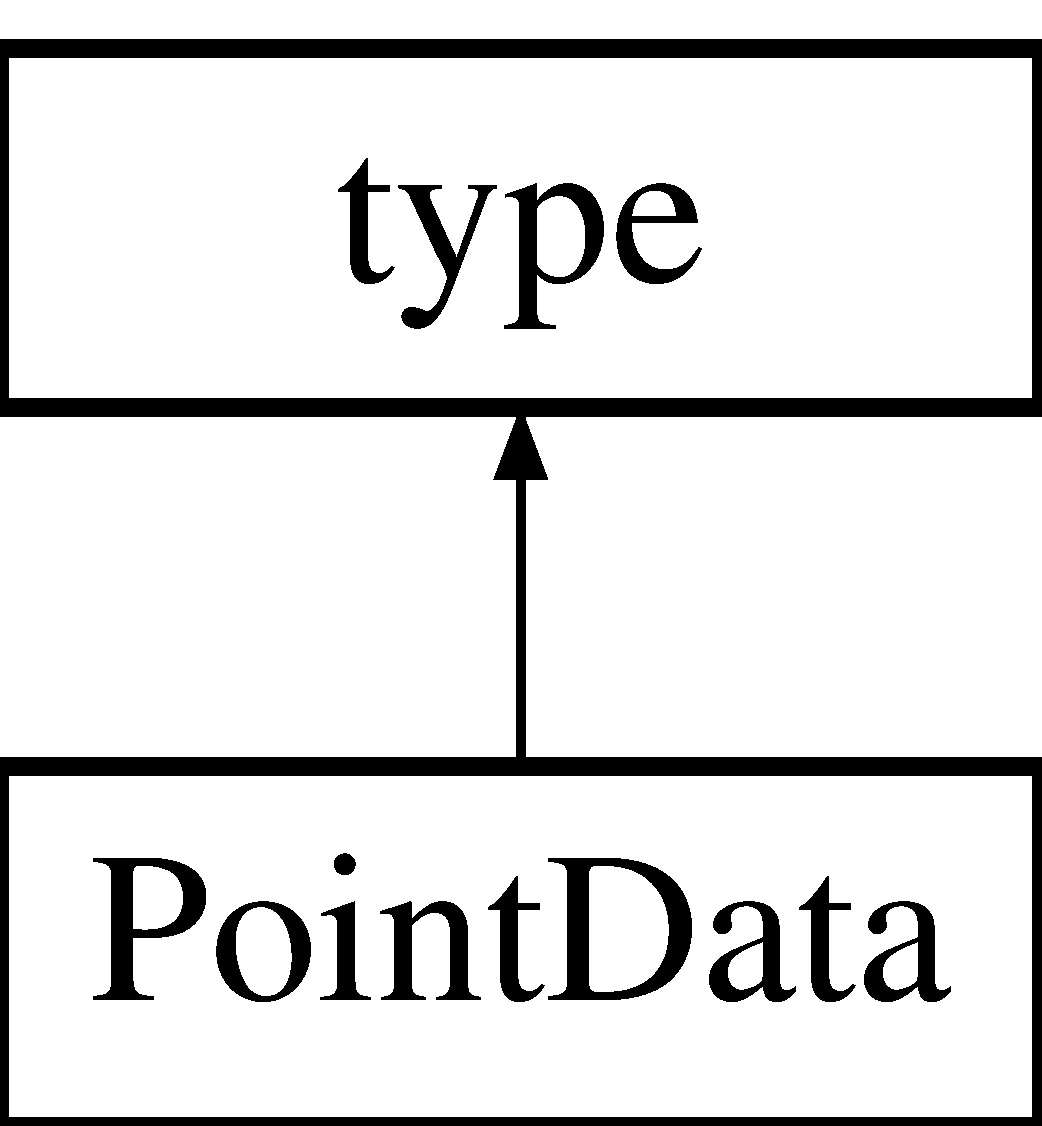
\includegraphics[height=2.000000cm]{classPointData}
\end{center}
\end{figure}
\subsection*{Public Member Functions}
\begin{DoxyCompactItemize}
\item 
virtual \hyperlink{classPointData_a53f701fd5abdb6105900c13f8282305e}{$\sim$\+Point\+Data} ()
\begin{DoxyCompactList}\small\item\em Destructor. \end{DoxyCompactList}\end{DoxyCompactItemize}
\subsection*{Data\+Array}
\label{_amgrp14411195be4ee927801b68cb96397add}%
Accessor and modifier functions for the Data\+Array sequence element. \begin{DoxyCompactItemize}
\item 
typedef \+::\hyperlink{classDataArray__t}{Data\+Array\+\_\+t} \hyperlink{classPointData_a249ad018361c7a9d61f42e1fc8af717f}{Data\+Array\+\_\+type}
\begin{DoxyCompactList}\small\item\em Element type. \end{DoxyCompactList}\item 
typedef \+::xsd\+::cxx\+::tree\+::sequence$<$ \hyperlink{classPointData_a249ad018361c7a9d61f42e1fc8af717f}{Data\+Array\+\_\+type} $>$ \hyperlink{classPointData_acd882fa412789571fcaa2599ad2b2c71}{Data\+Array\+\_\+sequence}
\begin{DoxyCompactList}\small\item\em Element sequence container type. \end{DoxyCompactList}\item 
typedef Data\+Array\+\_\+sequence\+::iterator \hyperlink{classPointData_afb66f793f2a65ca38e3cd8fa21eef701}{Data\+Array\+\_\+iterator}
\begin{DoxyCompactList}\small\item\em Element iterator type. \end{DoxyCompactList}\item 
typedef Data\+Array\+\_\+sequence\+::const\+\_\+iterator \hyperlink{classPointData_a6bd3313479b6a109e24bc9e7b306831b}{Data\+Array\+\_\+const\+\_\+iterator}
\begin{DoxyCompactList}\small\item\em Element constant iterator type. \end{DoxyCompactList}\item 
typedef \+::xsd\+::cxx\+::tree\+::traits$<$ \hyperlink{classPointData_a249ad018361c7a9d61f42e1fc8af717f}{Data\+Array\+\_\+type}, char $>$ \hyperlink{classPointData_ae9066a14984b6f7aa938ba2d58244055}{Data\+Array\+\_\+traits}
\begin{DoxyCompactList}\small\item\em Element traits type. \end{DoxyCompactList}\item 
const \hyperlink{classPointData_acd882fa412789571fcaa2599ad2b2c71}{Data\+Array\+\_\+sequence} \& \hyperlink{classPointData_ac4d75ba2976d6acdaceb0b69f574e895}{Data\+Array} () const 
\begin{DoxyCompactList}\small\item\em Return a read-\/only (constant) reference to the element sequence. \end{DoxyCompactList}\item 
\hyperlink{classPointData_acd882fa412789571fcaa2599ad2b2c71}{Data\+Array\+\_\+sequence} \& \hyperlink{classPointData_aa8ff7ad5b2c1d99794d4b96e481138d2}{Data\+Array} ()
\begin{DoxyCompactList}\small\item\em Return a read-\/write reference to the element sequence. \end{DoxyCompactList}\item 
void \hyperlink{classPointData_a207059b73203faf8b3fec8659a9104e5}{Data\+Array} (const \hyperlink{classPointData_acd882fa412789571fcaa2599ad2b2c71}{Data\+Array\+\_\+sequence} \&s)
\begin{DoxyCompactList}\small\item\em Copy elements from a given sequence. \end{DoxyCompactList}\end{DoxyCompactItemize}
\subsection*{Constructors}
\begin{DoxyCompactItemize}
\item 
\hyperlink{classPointData_add74ef42ae2c48850449cd59e216111f}{Point\+Data} ()
\begin{DoxyCompactList}\small\item\em Create an instance from the ultimate base and initializers for required elements and attributes. \end{DoxyCompactList}\item 
\hyperlink{classPointData_ae0d2a9251b2690a28a04a96105874e45}{Point\+Data} (const \+::xercesc\+::\+D\+O\+M\+Element \&e,\+::\hyperlink{namespacexml__schema_a8d981c127a1f5106d04ad5853e707361}{xml\+\_\+schema\+::flags} f=0,\+::\hyperlink{namespacexml__schema_a395f5179c5fc4643909d66e9ff28d8ca}{xml\+\_\+schema\+::container} $\ast$c=0)
\begin{DoxyCompactList}\small\item\em Create an instance from a D\+O\+M element. \end{DoxyCompactList}\item 
\hyperlink{classPointData_a552557267dd3178a8e76be436b0709bc}{Point\+Data} (const \hyperlink{classPointData}{Point\+Data} \&x,\+::\hyperlink{namespacexml__schema_a8d981c127a1f5106d04ad5853e707361}{xml\+\_\+schema\+::flags} f=0,\+::\hyperlink{namespacexml__schema_a395f5179c5fc4643909d66e9ff28d8ca}{xml\+\_\+schema\+::container} $\ast$c=0)
\begin{DoxyCompactList}\small\item\em Copy constructor. \end{DoxyCompactList}\item 
virtual \hyperlink{classPointData}{Point\+Data} $\ast$ \hyperlink{classPointData_aeb33ffedc35f8abc9ffd0d2f053c68ac}{\+\_\+clone} (\+::\hyperlink{namespacexml__schema_a8d981c127a1f5106d04ad5853e707361}{xml\+\_\+schema\+::flags} f=0,\+::\hyperlink{namespacexml__schema_a395f5179c5fc4643909d66e9ff28d8ca}{xml\+\_\+schema\+::container} $\ast$c=0) const 
\begin{DoxyCompactList}\small\item\em Copy the instance polymorphically. \end{DoxyCompactList}\end{DoxyCompactItemize}


\subsection{Detailed Description}
Class corresponding to the Point\+Data schema type. 

\subsection{Member Typedef Documentation}
\hypertarget{classPointData_a6bd3313479b6a109e24bc9e7b306831b}{}\index{Point\+Data@{Point\+Data}!Data\+Array\+\_\+const\+\_\+iterator@{Data\+Array\+\_\+const\+\_\+iterator}}
\index{Data\+Array\+\_\+const\+\_\+iterator@{Data\+Array\+\_\+const\+\_\+iterator}!Point\+Data@{Point\+Data}}
\subsubsection[{Data\+Array\+\_\+const\+\_\+iterator}]{\setlength{\rightskip}{0pt plus 5cm}typedef Data\+Array\+\_\+sequence\+::const\+\_\+iterator {\bf Point\+Data\+::\+Data\+Array\+\_\+const\+\_\+iterator}}\label{classPointData_a6bd3313479b6a109e24bc9e7b306831b}


Element constant iterator type. 

\hypertarget{classPointData_afb66f793f2a65ca38e3cd8fa21eef701}{}\index{Point\+Data@{Point\+Data}!Data\+Array\+\_\+iterator@{Data\+Array\+\_\+iterator}}
\index{Data\+Array\+\_\+iterator@{Data\+Array\+\_\+iterator}!Point\+Data@{Point\+Data}}
\subsubsection[{Data\+Array\+\_\+iterator}]{\setlength{\rightskip}{0pt plus 5cm}typedef Data\+Array\+\_\+sequence\+::iterator {\bf Point\+Data\+::\+Data\+Array\+\_\+iterator}}\label{classPointData_afb66f793f2a65ca38e3cd8fa21eef701}


Element iterator type. 

\hypertarget{classPointData_acd882fa412789571fcaa2599ad2b2c71}{}\index{Point\+Data@{Point\+Data}!Data\+Array\+\_\+sequence@{Data\+Array\+\_\+sequence}}
\index{Data\+Array\+\_\+sequence@{Data\+Array\+\_\+sequence}!Point\+Data@{Point\+Data}}
\subsubsection[{Data\+Array\+\_\+sequence}]{\setlength{\rightskip}{0pt plus 5cm}typedef \+::xsd\+::cxx\+::tree\+::sequence$<$ {\bf Data\+Array\+\_\+type} $>$ {\bf Point\+Data\+::\+Data\+Array\+\_\+sequence}}\label{classPointData_acd882fa412789571fcaa2599ad2b2c71}


Element sequence container type. 

\hypertarget{classPointData_ae9066a14984b6f7aa938ba2d58244055}{}\index{Point\+Data@{Point\+Data}!Data\+Array\+\_\+traits@{Data\+Array\+\_\+traits}}
\index{Data\+Array\+\_\+traits@{Data\+Array\+\_\+traits}!Point\+Data@{Point\+Data}}
\subsubsection[{Data\+Array\+\_\+traits}]{\setlength{\rightskip}{0pt plus 5cm}typedef \+::xsd\+::cxx\+::tree\+::traits$<$ {\bf Data\+Array\+\_\+type}, char $>$ {\bf Point\+Data\+::\+Data\+Array\+\_\+traits}}\label{classPointData_ae9066a14984b6f7aa938ba2d58244055}


Element traits type. 

\hypertarget{classPointData_a249ad018361c7a9d61f42e1fc8af717f}{}\index{Point\+Data@{Point\+Data}!Data\+Array\+\_\+type@{Data\+Array\+\_\+type}}
\index{Data\+Array\+\_\+type@{Data\+Array\+\_\+type}!Point\+Data@{Point\+Data}}
\subsubsection[{Data\+Array\+\_\+type}]{\setlength{\rightskip}{0pt plus 5cm}typedef \+::{\bf Data\+Array\+\_\+t} {\bf Point\+Data\+::\+Data\+Array\+\_\+type}}\label{classPointData_a249ad018361c7a9d61f42e1fc8af717f}


Element type. 



\subsection{Constructor \& Destructor Documentation}
\hypertarget{classPointData_add74ef42ae2c48850449cd59e216111f}{}\index{Point\+Data@{Point\+Data}!Point\+Data@{Point\+Data}}
\index{Point\+Data@{Point\+Data}!Point\+Data@{Point\+Data}}
\subsubsection[{Point\+Data}]{\setlength{\rightskip}{0pt plus 5cm}Point\+Data\+::\+Point\+Data (
\begin{DoxyParamCaption}
{}
\end{DoxyParamCaption}
)}\label{classPointData_add74ef42ae2c48850449cd59e216111f}


Create an instance from the ultimate base and initializers for required elements and attributes. 

\hypertarget{classPointData_ae0d2a9251b2690a28a04a96105874e45}{}\index{Point\+Data@{Point\+Data}!Point\+Data@{Point\+Data}}
\index{Point\+Data@{Point\+Data}!Point\+Data@{Point\+Data}}
\subsubsection[{Point\+Data}]{\setlength{\rightskip}{0pt plus 5cm}Point\+Data\+::\+Point\+Data (
\begin{DoxyParamCaption}
\item[{const \+::xercesc\+::\+D\+O\+M\+Element \&}]{e, }
\item[{\+::{\bf xml\+\_\+schema\+::flags}}]{f = {\ttfamily 0}, }
\item[{\+::{\bf xml\+\_\+schema\+::container} $\ast$}]{c = {\ttfamily 0}}
\end{DoxyParamCaption}
)}\label{classPointData_ae0d2a9251b2690a28a04a96105874e45}


Create an instance from a D\+O\+M element. 


\begin{DoxyParams}{Parameters}
{\em e} & A D\+O\+M element to extract the data from. \\
\hline
{\em f} & Flags to create the new instance with. \\
\hline
{\em c} & A pointer to the object that will contain the new instance. \\
\hline
\end{DoxyParams}
\hypertarget{classPointData_a552557267dd3178a8e76be436b0709bc}{}\index{Point\+Data@{Point\+Data}!Point\+Data@{Point\+Data}}
\index{Point\+Data@{Point\+Data}!Point\+Data@{Point\+Data}}
\subsubsection[{Point\+Data}]{\setlength{\rightskip}{0pt plus 5cm}Point\+Data\+::\+Point\+Data (
\begin{DoxyParamCaption}
\item[{const {\bf Point\+Data} \&}]{x, }
\item[{\+::{\bf xml\+\_\+schema\+::flags}}]{f = {\ttfamily 0}, }
\item[{\+::{\bf xml\+\_\+schema\+::container} $\ast$}]{c = {\ttfamily 0}}
\end{DoxyParamCaption}
)}\label{classPointData_a552557267dd3178a8e76be436b0709bc}


Copy constructor. 


\begin{DoxyParams}{Parameters}
{\em x} & An instance to make a copy of. \\
\hline
{\em f} & Flags to create the copy with. \\
\hline
{\em c} & A pointer to the object that will contain the copy.\\
\hline
\end{DoxyParams}
For polymorphic object models use the {\ttfamily \+\_\+clone} function instead. \hypertarget{classPointData_a53f701fd5abdb6105900c13f8282305e}{}\index{Point\+Data@{Point\+Data}!````~Point\+Data@{$\sim$\+Point\+Data}}
\index{````~Point\+Data@{$\sim$\+Point\+Data}!Point\+Data@{Point\+Data}}
\subsubsection[{$\sim$\+Point\+Data}]{\setlength{\rightskip}{0pt plus 5cm}Point\+Data\+::$\sim$\+Point\+Data (
\begin{DoxyParamCaption}
{}
\end{DoxyParamCaption}
)\hspace{0.3cm}{\ttfamily [virtual]}}\label{classPointData_a53f701fd5abdb6105900c13f8282305e}


Destructor. 



\subsection{Member Function Documentation}
\hypertarget{classPointData_aeb33ffedc35f8abc9ffd0d2f053c68ac}{}\index{Point\+Data@{Point\+Data}!\+\_\+clone@{\+\_\+clone}}
\index{\+\_\+clone@{\+\_\+clone}!Point\+Data@{Point\+Data}}
\subsubsection[{\+\_\+clone}]{\setlength{\rightskip}{0pt plus 5cm}{\bf Point\+Data} $\ast$ Point\+Data\+::\+\_\+clone (
\begin{DoxyParamCaption}
\item[{\+::{\bf xml\+\_\+schema\+::flags}}]{f = {\ttfamily 0}, }
\item[{\+::{\bf xml\+\_\+schema\+::container} $\ast$}]{c = {\ttfamily 0}}
\end{DoxyParamCaption}
) const\hspace{0.3cm}{\ttfamily [virtual]}}\label{classPointData_aeb33ffedc35f8abc9ffd0d2f053c68ac}


Copy the instance polymorphically. 


\begin{DoxyParams}{Parameters}
{\em f} & Flags to create the copy with. \\
\hline
{\em c} & A pointer to the object that will contain the copy. \\
\hline
\end{DoxyParams}
\begin{DoxyReturn}{Returns}
A pointer to the dynamically allocated copy.
\end{DoxyReturn}
This function ensures that the dynamic type of the instance is used for copying and should be used for polymorphic object models instead of the copy constructor. \hypertarget{classPointData_ac4d75ba2976d6acdaceb0b69f574e895}{}\index{Point\+Data@{Point\+Data}!Data\+Array@{Data\+Array}}
\index{Data\+Array@{Data\+Array}!Point\+Data@{Point\+Data}}
\subsubsection[{Data\+Array}]{\setlength{\rightskip}{0pt plus 5cm}const {\bf Point\+Data\+::\+Data\+Array\+\_\+sequence} \& Point\+Data\+::\+Data\+Array (
\begin{DoxyParamCaption}
{}
\end{DoxyParamCaption}
) const}\label{classPointData_ac4d75ba2976d6acdaceb0b69f574e895}


Return a read-\/only (constant) reference to the element sequence. 

\begin{DoxyReturn}{Returns}
A constant reference to the sequence container. 
\end{DoxyReturn}
\hypertarget{classPointData_aa8ff7ad5b2c1d99794d4b96e481138d2}{}\index{Point\+Data@{Point\+Data}!Data\+Array@{Data\+Array}}
\index{Data\+Array@{Data\+Array}!Point\+Data@{Point\+Data}}
\subsubsection[{Data\+Array}]{\setlength{\rightskip}{0pt plus 5cm}{\bf Point\+Data\+::\+Data\+Array\+\_\+sequence} \& Point\+Data\+::\+Data\+Array (
\begin{DoxyParamCaption}
{}
\end{DoxyParamCaption}
)}\label{classPointData_aa8ff7ad5b2c1d99794d4b96e481138d2}


Return a read-\/write reference to the element sequence. 

\begin{DoxyReturn}{Returns}
A reference to the sequence container. 
\end{DoxyReturn}
\hypertarget{classPointData_a207059b73203faf8b3fec8659a9104e5}{}\index{Point\+Data@{Point\+Data}!Data\+Array@{Data\+Array}}
\index{Data\+Array@{Data\+Array}!Point\+Data@{Point\+Data}}
\subsubsection[{Data\+Array}]{\setlength{\rightskip}{0pt plus 5cm}void Point\+Data\+::\+Data\+Array (
\begin{DoxyParamCaption}
\item[{const {\bf Data\+Array\+\_\+sequence} \&}]{s}
\end{DoxyParamCaption}
)}\label{classPointData_a207059b73203faf8b3fec8659a9104e5}


Copy elements from a given sequence. 


\begin{DoxyParams}{Parameters}
{\em s} & A sequence to copy elements from.\\
\hline
\end{DoxyParams}
For each element in {\itshape s} this function makes a copy and adds it to the sequence. Note that this operation completely changes the sequence and all old elements will be lost. 

The documentation for this class was generated from the following files\+:\begin{DoxyCompactItemize}
\item 
src/output\+Writer/\hyperlink{vtk-unstructured_8h}{vtk-\/unstructured.\+h}\item 
src/output\+Writer/\hyperlink{vtk-unstructured_8cpp}{vtk-\/unstructured.\+cpp}\end{DoxyCompactItemize}

\hypertarget{classPoints}{}\section{Points Class Reference}
\label{classPoints}\index{Points@{Points}}


Class corresponding to the Points schema type.  




{\ttfamily \#include $<$vtk-\/unstructured.\+h$>$}

Inheritance diagram for Points\+:\begin{figure}[H]
\begin{center}
\leavevmode
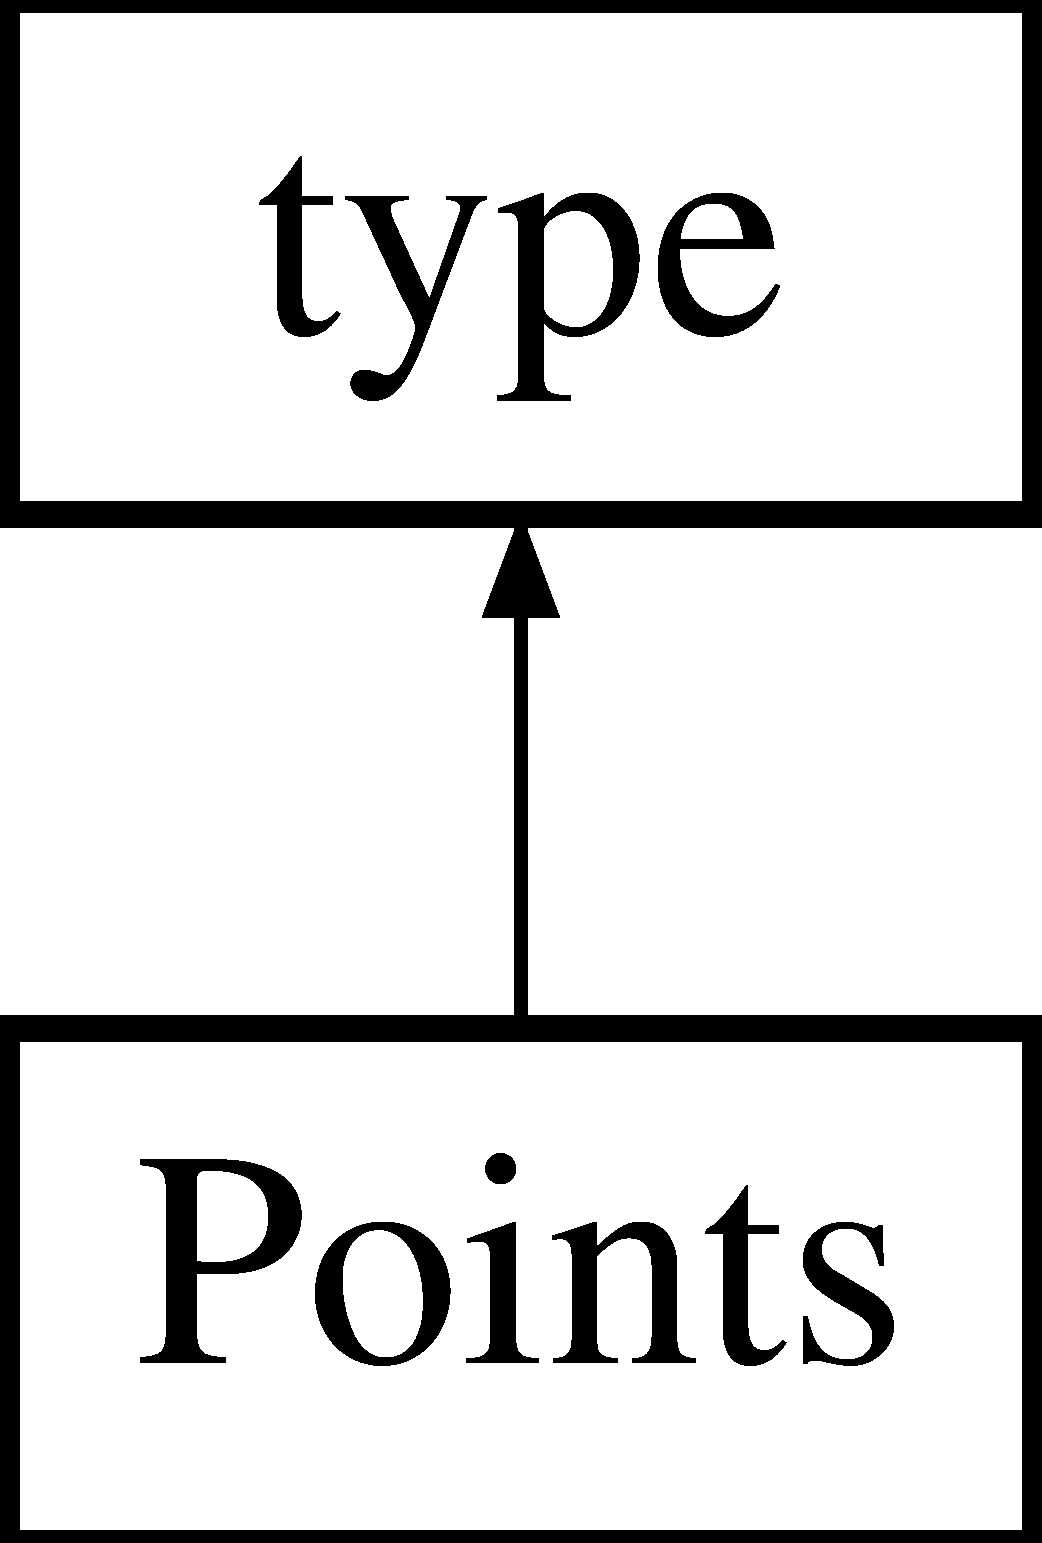
\includegraphics[height=2.000000cm]{classPoints}
\end{center}
\end{figure}
\subsection*{Public Member Functions}
\begin{DoxyCompactItemize}
\item 
virtual \hyperlink{classPoints_a9d56d7dc8b6a6f492e07d354eb379c12}{$\sim$\+Points} ()
\begin{DoxyCompactList}\small\item\em Destructor. \end{DoxyCompactList}\end{DoxyCompactItemize}
\subsection*{Data\+Array}
\label{_amgrp14411195be4ee927801b68cb96397add}%
Accessor and modifier functions for the Data\+Array sequence element. \begin{DoxyCompactItemize}
\item 
typedef \+::\hyperlink{classDataArray__t}{Data\+Array\+\_\+t} \hyperlink{classPoints_a6afedf501b722fe7d7ffeae03ece6238}{Data\+Array\+\_\+type}
\begin{DoxyCompactList}\small\item\em Element type. \end{DoxyCompactList}\item 
typedef \+::xsd\+::cxx\+::tree\+::sequence$<$ \hyperlink{classPoints_a6afedf501b722fe7d7ffeae03ece6238}{Data\+Array\+\_\+type} $>$ \hyperlink{classPoints_ac8b51dcf0e7659ca61ff9b9d24051016}{Data\+Array\+\_\+sequence}
\begin{DoxyCompactList}\small\item\em Element sequence container type. \end{DoxyCompactList}\item 
typedef Data\+Array\+\_\+sequence\+::iterator \hyperlink{classPoints_ac4cd7a177b464c1e08d493600a7e6e16}{Data\+Array\+\_\+iterator}
\begin{DoxyCompactList}\small\item\em Element iterator type. \end{DoxyCompactList}\item 
typedef Data\+Array\+\_\+sequence\+::const\+\_\+iterator \hyperlink{classPoints_a795a395909c3360569fe0e854ba6059e}{Data\+Array\+\_\+const\+\_\+iterator}
\begin{DoxyCompactList}\small\item\em Element constant iterator type. \end{DoxyCompactList}\item 
typedef \+::xsd\+::cxx\+::tree\+::traits$<$ \hyperlink{classPoints_a6afedf501b722fe7d7ffeae03ece6238}{Data\+Array\+\_\+type}, char $>$ \hyperlink{classPoints_a815b88c9204c7251f4a08c6769645ef1}{Data\+Array\+\_\+traits}
\begin{DoxyCompactList}\small\item\em Element traits type. \end{DoxyCompactList}\item 
const \hyperlink{classPoints_ac8b51dcf0e7659ca61ff9b9d24051016}{Data\+Array\+\_\+sequence} \& \hyperlink{classPoints_a86c60a0068ebdb8d3e8cbe9fa8f35f55}{Data\+Array} () const 
\begin{DoxyCompactList}\small\item\em Return a read-\/only (constant) reference to the element sequence. \end{DoxyCompactList}\item 
\hyperlink{classPoints_ac8b51dcf0e7659ca61ff9b9d24051016}{Data\+Array\+\_\+sequence} \& \hyperlink{classPoints_a3fdfb1b1b2f1221ad50ba5087826177c}{Data\+Array} ()
\begin{DoxyCompactList}\small\item\em Return a read-\/write reference to the element sequence. \end{DoxyCompactList}\item 
void \hyperlink{classPoints_aa22a86fe31d5f903be59dda3de92bb67}{Data\+Array} (const \hyperlink{classPoints_ac8b51dcf0e7659ca61ff9b9d24051016}{Data\+Array\+\_\+sequence} \&s)
\begin{DoxyCompactList}\small\item\em Copy elements from a given sequence. \end{DoxyCompactList}\end{DoxyCompactItemize}
\subsection*{Constructors}
\begin{DoxyCompactItemize}
\item 
\hyperlink{classPoints_aa4e68083d98bd04233c9753dfe1e46ab}{Points} ()
\begin{DoxyCompactList}\small\item\em Create an instance from the ultimate base and initializers for required elements and attributes. \end{DoxyCompactList}\item 
\hyperlink{classPoints_a36a1ac8ea9ac092adff2888915e81304}{Points} (const \+::xercesc\+::\+D\+O\+M\+Element \&e,\+::\hyperlink{namespacexml__schema_a8d981c127a1f5106d04ad5853e707361}{xml\+\_\+schema\+::flags} f=0,\+::\hyperlink{namespacexml__schema_a395f5179c5fc4643909d66e9ff28d8ca}{xml\+\_\+schema\+::container} $\ast$c=0)
\begin{DoxyCompactList}\small\item\em Create an instance from a D\+O\+M element. \end{DoxyCompactList}\item 
\hyperlink{classPoints_ad49b51469dc53b028c244a88bd9fb08b}{Points} (const \hyperlink{classPoints}{Points} \&x,\+::\hyperlink{namespacexml__schema_a8d981c127a1f5106d04ad5853e707361}{xml\+\_\+schema\+::flags} f=0,\+::\hyperlink{namespacexml__schema_a395f5179c5fc4643909d66e9ff28d8ca}{xml\+\_\+schema\+::container} $\ast$c=0)
\begin{DoxyCompactList}\small\item\em Copy constructor. \end{DoxyCompactList}\item 
virtual \hyperlink{classPoints}{Points} $\ast$ \hyperlink{classPoints_a5dff673c4b4a59465aee3ede80328ae9}{\+\_\+clone} (\+::\hyperlink{namespacexml__schema_a8d981c127a1f5106d04ad5853e707361}{xml\+\_\+schema\+::flags} f=0,\+::\hyperlink{namespacexml__schema_a395f5179c5fc4643909d66e9ff28d8ca}{xml\+\_\+schema\+::container} $\ast$c=0) const 
\begin{DoxyCompactList}\small\item\em Copy the instance polymorphically. \end{DoxyCompactList}\end{DoxyCompactItemize}


\subsection{Detailed Description}
Class corresponding to the Points schema type. 

\subsection{Member Typedef Documentation}
\hypertarget{classPoints_a795a395909c3360569fe0e854ba6059e}{}\index{Points@{Points}!Data\+Array\+\_\+const\+\_\+iterator@{Data\+Array\+\_\+const\+\_\+iterator}}
\index{Data\+Array\+\_\+const\+\_\+iterator@{Data\+Array\+\_\+const\+\_\+iterator}!Points@{Points}}
\subsubsection[{Data\+Array\+\_\+const\+\_\+iterator}]{\setlength{\rightskip}{0pt plus 5cm}typedef Data\+Array\+\_\+sequence\+::const\+\_\+iterator {\bf Points\+::\+Data\+Array\+\_\+const\+\_\+iterator}}\label{classPoints_a795a395909c3360569fe0e854ba6059e}


Element constant iterator type. 

\hypertarget{classPoints_ac4cd7a177b464c1e08d493600a7e6e16}{}\index{Points@{Points}!Data\+Array\+\_\+iterator@{Data\+Array\+\_\+iterator}}
\index{Data\+Array\+\_\+iterator@{Data\+Array\+\_\+iterator}!Points@{Points}}
\subsubsection[{Data\+Array\+\_\+iterator}]{\setlength{\rightskip}{0pt plus 5cm}typedef Data\+Array\+\_\+sequence\+::iterator {\bf Points\+::\+Data\+Array\+\_\+iterator}}\label{classPoints_ac4cd7a177b464c1e08d493600a7e6e16}


Element iterator type. 

\hypertarget{classPoints_ac8b51dcf0e7659ca61ff9b9d24051016}{}\index{Points@{Points}!Data\+Array\+\_\+sequence@{Data\+Array\+\_\+sequence}}
\index{Data\+Array\+\_\+sequence@{Data\+Array\+\_\+sequence}!Points@{Points}}
\subsubsection[{Data\+Array\+\_\+sequence}]{\setlength{\rightskip}{0pt plus 5cm}typedef \+::xsd\+::cxx\+::tree\+::sequence$<$ {\bf Data\+Array\+\_\+type} $>$ {\bf Points\+::\+Data\+Array\+\_\+sequence}}\label{classPoints_ac8b51dcf0e7659ca61ff9b9d24051016}


Element sequence container type. 

\hypertarget{classPoints_a815b88c9204c7251f4a08c6769645ef1}{}\index{Points@{Points}!Data\+Array\+\_\+traits@{Data\+Array\+\_\+traits}}
\index{Data\+Array\+\_\+traits@{Data\+Array\+\_\+traits}!Points@{Points}}
\subsubsection[{Data\+Array\+\_\+traits}]{\setlength{\rightskip}{0pt plus 5cm}typedef \+::xsd\+::cxx\+::tree\+::traits$<$ {\bf Data\+Array\+\_\+type}, char $>$ {\bf Points\+::\+Data\+Array\+\_\+traits}}\label{classPoints_a815b88c9204c7251f4a08c6769645ef1}


Element traits type. 

\hypertarget{classPoints_a6afedf501b722fe7d7ffeae03ece6238}{}\index{Points@{Points}!Data\+Array\+\_\+type@{Data\+Array\+\_\+type}}
\index{Data\+Array\+\_\+type@{Data\+Array\+\_\+type}!Points@{Points}}
\subsubsection[{Data\+Array\+\_\+type}]{\setlength{\rightskip}{0pt plus 5cm}typedef \+::{\bf Data\+Array\+\_\+t} {\bf Points\+::\+Data\+Array\+\_\+type}}\label{classPoints_a6afedf501b722fe7d7ffeae03ece6238}


Element type. 



\subsection{Constructor \& Destructor Documentation}
\hypertarget{classPoints_aa4e68083d98bd04233c9753dfe1e46ab}{}\index{Points@{Points}!Points@{Points}}
\index{Points@{Points}!Points@{Points}}
\subsubsection[{Points}]{\setlength{\rightskip}{0pt plus 5cm}Points\+::\+Points (
\begin{DoxyParamCaption}
{}
\end{DoxyParamCaption}
)}\label{classPoints_aa4e68083d98bd04233c9753dfe1e46ab}


Create an instance from the ultimate base and initializers for required elements and attributes. 

\hypertarget{classPoints_a36a1ac8ea9ac092adff2888915e81304}{}\index{Points@{Points}!Points@{Points}}
\index{Points@{Points}!Points@{Points}}
\subsubsection[{Points}]{\setlength{\rightskip}{0pt plus 5cm}Points\+::\+Points (
\begin{DoxyParamCaption}
\item[{const \+::xercesc\+::\+D\+O\+M\+Element \&}]{e, }
\item[{\+::{\bf xml\+\_\+schema\+::flags}}]{f = {\ttfamily 0}, }
\item[{\+::{\bf xml\+\_\+schema\+::container} $\ast$}]{c = {\ttfamily 0}}
\end{DoxyParamCaption}
)}\label{classPoints_a36a1ac8ea9ac092adff2888915e81304}


Create an instance from a D\+O\+M element. 


\begin{DoxyParams}{Parameters}
{\em e} & A D\+O\+M element to extract the data from. \\
\hline
{\em f} & Flags to create the new instance with. \\
\hline
{\em c} & A pointer to the object that will contain the new instance. \\
\hline
\end{DoxyParams}
\hypertarget{classPoints_ad49b51469dc53b028c244a88bd9fb08b}{}\index{Points@{Points}!Points@{Points}}
\index{Points@{Points}!Points@{Points}}
\subsubsection[{Points}]{\setlength{\rightskip}{0pt plus 5cm}Points\+::\+Points (
\begin{DoxyParamCaption}
\item[{const {\bf Points} \&}]{x, }
\item[{\+::{\bf xml\+\_\+schema\+::flags}}]{f = {\ttfamily 0}, }
\item[{\+::{\bf xml\+\_\+schema\+::container} $\ast$}]{c = {\ttfamily 0}}
\end{DoxyParamCaption}
)}\label{classPoints_ad49b51469dc53b028c244a88bd9fb08b}


Copy constructor. 


\begin{DoxyParams}{Parameters}
{\em x} & An instance to make a copy of. \\
\hline
{\em f} & Flags to create the copy with. \\
\hline
{\em c} & A pointer to the object that will contain the copy.\\
\hline
\end{DoxyParams}
For polymorphic object models use the {\ttfamily \+\_\+clone} function instead. \hypertarget{classPoints_a9d56d7dc8b6a6f492e07d354eb379c12}{}\index{Points@{Points}!````~Points@{$\sim$\+Points}}
\index{````~Points@{$\sim$\+Points}!Points@{Points}}
\subsubsection[{$\sim$\+Points}]{\setlength{\rightskip}{0pt plus 5cm}Points\+::$\sim$\+Points (
\begin{DoxyParamCaption}
{}
\end{DoxyParamCaption}
)\hspace{0.3cm}{\ttfamily [virtual]}}\label{classPoints_a9d56d7dc8b6a6f492e07d354eb379c12}


Destructor. 



\subsection{Member Function Documentation}
\hypertarget{classPoints_a5dff673c4b4a59465aee3ede80328ae9}{}\index{Points@{Points}!\+\_\+clone@{\+\_\+clone}}
\index{\+\_\+clone@{\+\_\+clone}!Points@{Points}}
\subsubsection[{\+\_\+clone}]{\setlength{\rightskip}{0pt plus 5cm}{\bf Points} $\ast$ Points\+::\+\_\+clone (
\begin{DoxyParamCaption}
\item[{\+::{\bf xml\+\_\+schema\+::flags}}]{f = {\ttfamily 0}, }
\item[{\+::{\bf xml\+\_\+schema\+::container} $\ast$}]{c = {\ttfamily 0}}
\end{DoxyParamCaption}
) const\hspace{0.3cm}{\ttfamily [virtual]}}\label{classPoints_a5dff673c4b4a59465aee3ede80328ae9}


Copy the instance polymorphically. 


\begin{DoxyParams}{Parameters}
{\em f} & Flags to create the copy with. \\
\hline
{\em c} & A pointer to the object that will contain the copy. \\
\hline
\end{DoxyParams}
\begin{DoxyReturn}{Returns}
A pointer to the dynamically allocated copy.
\end{DoxyReturn}
This function ensures that the dynamic type of the instance is used for copying and should be used for polymorphic object models instead of the copy constructor. \hypertarget{classPoints_a86c60a0068ebdb8d3e8cbe9fa8f35f55}{}\index{Points@{Points}!Data\+Array@{Data\+Array}}
\index{Data\+Array@{Data\+Array}!Points@{Points}}
\subsubsection[{Data\+Array}]{\setlength{\rightskip}{0pt plus 5cm}const {\bf Points\+::\+Data\+Array\+\_\+sequence} \& Points\+::\+Data\+Array (
\begin{DoxyParamCaption}
{}
\end{DoxyParamCaption}
) const}\label{classPoints_a86c60a0068ebdb8d3e8cbe9fa8f35f55}


Return a read-\/only (constant) reference to the element sequence. 

\begin{DoxyReturn}{Returns}
A constant reference to the sequence container. 
\end{DoxyReturn}
\hypertarget{classPoints_a3fdfb1b1b2f1221ad50ba5087826177c}{}\index{Points@{Points}!Data\+Array@{Data\+Array}}
\index{Data\+Array@{Data\+Array}!Points@{Points}}
\subsubsection[{Data\+Array}]{\setlength{\rightskip}{0pt plus 5cm}{\bf Points\+::\+Data\+Array\+\_\+sequence} \& Points\+::\+Data\+Array (
\begin{DoxyParamCaption}
{}
\end{DoxyParamCaption}
)}\label{classPoints_a3fdfb1b1b2f1221ad50ba5087826177c}


Return a read-\/write reference to the element sequence. 

\begin{DoxyReturn}{Returns}
A reference to the sequence container. 
\end{DoxyReturn}
\hypertarget{classPoints_aa22a86fe31d5f903be59dda3de92bb67}{}\index{Points@{Points}!Data\+Array@{Data\+Array}}
\index{Data\+Array@{Data\+Array}!Points@{Points}}
\subsubsection[{Data\+Array}]{\setlength{\rightskip}{0pt plus 5cm}void Points\+::\+Data\+Array (
\begin{DoxyParamCaption}
\item[{const {\bf Data\+Array\+\_\+sequence} \&}]{s}
\end{DoxyParamCaption}
)}\label{classPoints_aa22a86fe31d5f903be59dda3de92bb67}


Copy elements from a given sequence. 


\begin{DoxyParams}{Parameters}
{\em s} & A sequence to copy elements from.\\
\hline
\end{DoxyParams}
For each element in {\itshape s} this function makes a copy and adds it to the sequence. Note that this operation completely changes the sequence and all old elements will be lost. 

The documentation for this class was generated from the following files\+:\begin{DoxyCompactItemize}
\item 
src/output\+Writer/\hyperlink{vtk-unstructured_8h}{vtk-\/unstructured.\+h}\item 
src/output\+Writer/\hyperlink{vtk-unstructured_8cpp}{vtk-\/unstructured.\+cpp}\end{DoxyCompactItemize}

\hypertarget{classPolyData__t}{}\section{Poly\+Data\+\_\+t Class Reference}
\label{classPolyData__t}\index{Poly\+Data\+\_\+t@{Poly\+Data\+\_\+t}}


Class corresponding to the Poly\+Data\+\_\+t schema type.  




{\ttfamily \#include $<$vtk-\/unstructured.\+h$>$}

Inheritance diagram for Poly\+Data\+\_\+t\+:\begin{figure}[H]
\begin{center}
\leavevmode
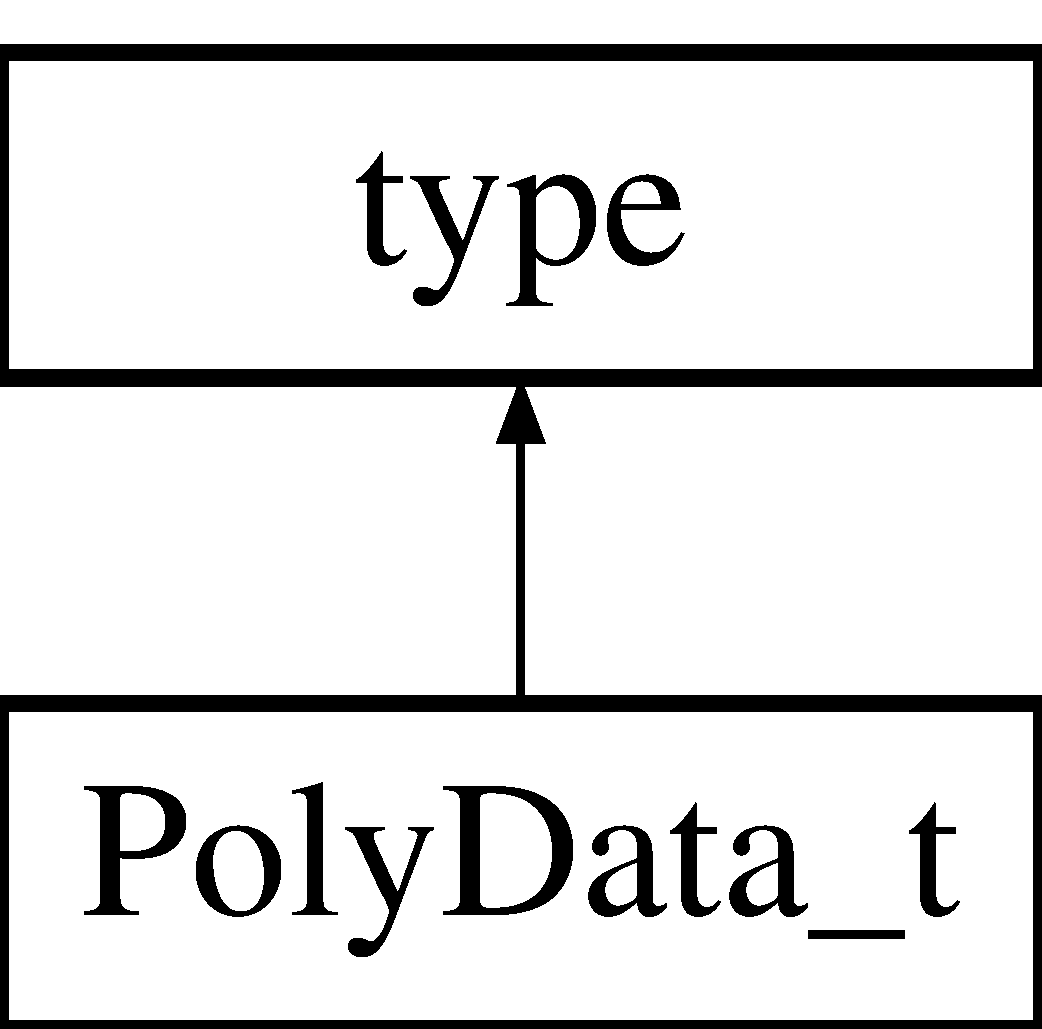
\includegraphics[height=2.000000cm]{classPolyData__t}
\end{center}
\end{figure}
\subsection*{Public Member Functions}
\begin{DoxyCompactItemize}
\item 
virtual \hyperlink{classPolyData__t_afefe18d998d21a0557e30c06b4089b99}{$\sim$\+Poly\+Data\+\_\+t} ()
\begin{DoxyCompactList}\small\item\em Destructor. \end{DoxyCompactList}\end{DoxyCompactItemize}
\subsection*{greeting}
\label{_amgrp699e0311097c48b46019dcfc07c772a1}%
Accessor and modifier functions for the greeting required element. \begin{DoxyCompactItemize}
\item 
typedef \+::\hyperlink{namespacexml__schema_aefbaf353f9a0043af46d23d9040ef268}{xml\+\_\+schema\+::string} \hyperlink{classPolyData__t_ae1f86bd7b6a37a0d0851de8a44627177}{greeting\+\_\+type}
\begin{DoxyCompactList}\small\item\em Element type. \end{DoxyCompactList}\item 
typedef \+::xsd\+::cxx\+::tree\+::traits$<$ \hyperlink{classPolyData__t_ae1f86bd7b6a37a0d0851de8a44627177}{greeting\+\_\+type}, char $>$ \hyperlink{classPolyData__t_a0825d12eafceffcedbb147730b8bf8a6}{greeting\+\_\+traits}
\begin{DoxyCompactList}\small\item\em Element traits type. \end{DoxyCompactList}\item 
const \hyperlink{classPolyData__t_ae1f86bd7b6a37a0d0851de8a44627177}{greeting\+\_\+type} \& \hyperlink{classPolyData__t_acce3e6cf99db0b383320a0ccfd62789f}{greeting} () const 
\begin{DoxyCompactList}\small\item\em Return a read-\/only (constant) reference to the element. \end{DoxyCompactList}\item 
\hyperlink{classPolyData__t_ae1f86bd7b6a37a0d0851de8a44627177}{greeting\+\_\+type} \& \hyperlink{classPolyData__t_a3879d9f3b0b8ae707f1c2465bbbcf507}{greeting} ()
\begin{DoxyCompactList}\small\item\em Return a read-\/write reference to the element. \end{DoxyCompactList}\item 
void \hyperlink{classPolyData__t_a23d6e1490860af1f76f135efb37510e1}{greeting} (const \hyperlink{classPolyData__t_ae1f86bd7b6a37a0d0851de8a44627177}{greeting\+\_\+type} \&x)
\begin{DoxyCompactList}\small\item\em Set the element value. \end{DoxyCompactList}\item 
void \hyperlink{classPolyData__t_a27c66fbcb156a64615e29b1082facd00}{greeting} (\+::std\+::auto\+\_\+ptr$<$ \hyperlink{classPolyData__t_ae1f86bd7b6a37a0d0851de8a44627177}{greeting\+\_\+type} $>$ p)
\begin{DoxyCompactList}\small\item\em Set the element value without copying. \end{DoxyCompactList}\end{DoxyCompactItemize}
\subsection*{Constructors}
\begin{DoxyCompactItemize}
\item 
\hyperlink{classPolyData__t_a4da6cc1205eee54feaebde53665f0621}{Poly\+Data\+\_\+t} (const \hyperlink{classPolyData__t_ae1f86bd7b6a37a0d0851de8a44627177}{greeting\+\_\+type} \&)
\begin{DoxyCompactList}\small\item\em Create an instance from the ultimate base and initializers for required elements and attributes. \end{DoxyCompactList}\item 
\hyperlink{classPolyData__t_a47b921cff0546cc9502c008a219d0058}{Poly\+Data\+\_\+t} (const \+::xercesc\+::\+D\+O\+M\+Element \&e,\+::\hyperlink{namespacexml__schema_a8d981c127a1f5106d04ad5853e707361}{xml\+\_\+schema\+::flags} f=0,\+::\hyperlink{namespacexml__schema_a395f5179c5fc4643909d66e9ff28d8ca}{xml\+\_\+schema\+::container} $\ast$c=0)
\begin{DoxyCompactList}\small\item\em Create an instance from a D\+O\+M element. \end{DoxyCompactList}\item 
\hyperlink{classPolyData__t_a6a0cccceec7668fe2f28776a4898a009}{Poly\+Data\+\_\+t} (const \hyperlink{classPolyData__t}{Poly\+Data\+\_\+t} \&x,\+::\hyperlink{namespacexml__schema_a8d981c127a1f5106d04ad5853e707361}{xml\+\_\+schema\+::flags} f=0,\+::\hyperlink{namespacexml__schema_a395f5179c5fc4643909d66e9ff28d8ca}{xml\+\_\+schema\+::container} $\ast$c=0)
\begin{DoxyCompactList}\small\item\em Copy constructor. \end{DoxyCompactList}\item 
virtual \hyperlink{classPolyData__t}{Poly\+Data\+\_\+t} $\ast$ \hyperlink{classPolyData__t_a90079722e663d849db7dec71493ddffe}{\+\_\+clone} (\+::\hyperlink{namespacexml__schema_a8d981c127a1f5106d04ad5853e707361}{xml\+\_\+schema\+::flags} f=0,\+::\hyperlink{namespacexml__schema_a395f5179c5fc4643909d66e9ff28d8ca}{xml\+\_\+schema\+::container} $\ast$c=0) const 
\begin{DoxyCompactList}\small\item\em Copy the instance polymorphically. \end{DoxyCompactList}\end{DoxyCompactItemize}


\subsection{Detailed Description}
Class corresponding to the Poly\+Data\+\_\+t schema type. 

\subsection{Member Typedef Documentation}
\hypertarget{classPolyData__t_a0825d12eafceffcedbb147730b8bf8a6}{}\index{Poly\+Data\+\_\+t@{Poly\+Data\+\_\+t}!greeting\+\_\+traits@{greeting\+\_\+traits}}
\index{greeting\+\_\+traits@{greeting\+\_\+traits}!Poly\+Data\+\_\+t@{Poly\+Data\+\_\+t}}
\subsubsection[{greeting\+\_\+traits}]{\setlength{\rightskip}{0pt plus 5cm}typedef \+::xsd\+::cxx\+::tree\+::traits$<$ {\bf greeting\+\_\+type}, char $>$ {\bf Poly\+Data\+\_\+t\+::greeting\+\_\+traits}}\label{classPolyData__t_a0825d12eafceffcedbb147730b8bf8a6}


Element traits type. 

\hypertarget{classPolyData__t_ae1f86bd7b6a37a0d0851de8a44627177}{}\index{Poly\+Data\+\_\+t@{Poly\+Data\+\_\+t}!greeting\+\_\+type@{greeting\+\_\+type}}
\index{greeting\+\_\+type@{greeting\+\_\+type}!Poly\+Data\+\_\+t@{Poly\+Data\+\_\+t}}
\subsubsection[{greeting\+\_\+type}]{\setlength{\rightskip}{0pt plus 5cm}typedef \+::{\bf xml\+\_\+schema\+::string} {\bf Poly\+Data\+\_\+t\+::greeting\+\_\+type}}\label{classPolyData__t_ae1f86bd7b6a37a0d0851de8a44627177}


Element type. 



\subsection{Constructor \& Destructor Documentation}
\hypertarget{classPolyData__t_a4da6cc1205eee54feaebde53665f0621}{}\index{Poly\+Data\+\_\+t@{Poly\+Data\+\_\+t}!Poly\+Data\+\_\+t@{Poly\+Data\+\_\+t}}
\index{Poly\+Data\+\_\+t@{Poly\+Data\+\_\+t}!Poly\+Data\+\_\+t@{Poly\+Data\+\_\+t}}
\subsubsection[{Poly\+Data\+\_\+t}]{\setlength{\rightskip}{0pt plus 5cm}Poly\+Data\+\_\+t\+::\+Poly\+Data\+\_\+t (
\begin{DoxyParamCaption}
\item[{const {\bf greeting\+\_\+type} \&}]{greeting}
\end{DoxyParamCaption}
)}\label{classPolyData__t_a4da6cc1205eee54feaebde53665f0621}


Create an instance from the ultimate base and initializers for required elements and attributes. 

\hypertarget{classPolyData__t_a47b921cff0546cc9502c008a219d0058}{}\index{Poly\+Data\+\_\+t@{Poly\+Data\+\_\+t}!Poly\+Data\+\_\+t@{Poly\+Data\+\_\+t}}
\index{Poly\+Data\+\_\+t@{Poly\+Data\+\_\+t}!Poly\+Data\+\_\+t@{Poly\+Data\+\_\+t}}
\subsubsection[{Poly\+Data\+\_\+t}]{\setlength{\rightskip}{0pt plus 5cm}Poly\+Data\+\_\+t\+::\+Poly\+Data\+\_\+t (
\begin{DoxyParamCaption}
\item[{const \+::xercesc\+::\+D\+O\+M\+Element \&}]{e, }
\item[{\+::{\bf xml\+\_\+schema\+::flags}}]{f = {\ttfamily 0}, }
\item[{\+::{\bf xml\+\_\+schema\+::container} $\ast$}]{c = {\ttfamily 0}}
\end{DoxyParamCaption}
)}\label{classPolyData__t_a47b921cff0546cc9502c008a219d0058}


Create an instance from a D\+O\+M element. 


\begin{DoxyParams}{Parameters}
{\em e} & A D\+O\+M element to extract the data from. \\
\hline
{\em f} & Flags to create the new instance with. \\
\hline
{\em c} & A pointer to the object that will contain the new instance. \\
\hline
\end{DoxyParams}
\hypertarget{classPolyData__t_a6a0cccceec7668fe2f28776a4898a009}{}\index{Poly\+Data\+\_\+t@{Poly\+Data\+\_\+t}!Poly\+Data\+\_\+t@{Poly\+Data\+\_\+t}}
\index{Poly\+Data\+\_\+t@{Poly\+Data\+\_\+t}!Poly\+Data\+\_\+t@{Poly\+Data\+\_\+t}}
\subsubsection[{Poly\+Data\+\_\+t}]{\setlength{\rightskip}{0pt plus 5cm}Poly\+Data\+\_\+t\+::\+Poly\+Data\+\_\+t (
\begin{DoxyParamCaption}
\item[{const {\bf Poly\+Data\+\_\+t} \&}]{x, }
\item[{\+::{\bf xml\+\_\+schema\+::flags}}]{f = {\ttfamily 0}, }
\item[{\+::{\bf xml\+\_\+schema\+::container} $\ast$}]{c = {\ttfamily 0}}
\end{DoxyParamCaption}
)}\label{classPolyData__t_a6a0cccceec7668fe2f28776a4898a009}


Copy constructor. 


\begin{DoxyParams}{Parameters}
{\em x} & An instance to make a copy of. \\
\hline
{\em f} & Flags to create the copy with. \\
\hline
{\em c} & A pointer to the object that will contain the copy.\\
\hline
\end{DoxyParams}
For polymorphic object models use the {\ttfamily \+\_\+clone} function instead. \hypertarget{classPolyData__t_afefe18d998d21a0557e30c06b4089b99}{}\index{Poly\+Data\+\_\+t@{Poly\+Data\+\_\+t}!````~Poly\+Data\+\_\+t@{$\sim$\+Poly\+Data\+\_\+t}}
\index{````~Poly\+Data\+\_\+t@{$\sim$\+Poly\+Data\+\_\+t}!Poly\+Data\+\_\+t@{Poly\+Data\+\_\+t}}
\subsubsection[{$\sim$\+Poly\+Data\+\_\+t}]{\setlength{\rightskip}{0pt plus 5cm}Poly\+Data\+\_\+t\+::$\sim$\+Poly\+Data\+\_\+t (
\begin{DoxyParamCaption}
{}
\end{DoxyParamCaption}
)\hspace{0.3cm}{\ttfamily [virtual]}}\label{classPolyData__t_afefe18d998d21a0557e30c06b4089b99}


Destructor. 



\subsection{Member Function Documentation}
\hypertarget{classPolyData__t_a90079722e663d849db7dec71493ddffe}{}\index{Poly\+Data\+\_\+t@{Poly\+Data\+\_\+t}!\+\_\+clone@{\+\_\+clone}}
\index{\+\_\+clone@{\+\_\+clone}!Poly\+Data\+\_\+t@{Poly\+Data\+\_\+t}}
\subsubsection[{\+\_\+clone}]{\setlength{\rightskip}{0pt plus 5cm}{\bf Poly\+Data\+\_\+t} $\ast$ Poly\+Data\+\_\+t\+::\+\_\+clone (
\begin{DoxyParamCaption}
\item[{\+::{\bf xml\+\_\+schema\+::flags}}]{f = {\ttfamily 0}, }
\item[{\+::{\bf xml\+\_\+schema\+::container} $\ast$}]{c = {\ttfamily 0}}
\end{DoxyParamCaption}
) const\hspace{0.3cm}{\ttfamily [virtual]}}\label{classPolyData__t_a90079722e663d849db7dec71493ddffe}


Copy the instance polymorphically. 


\begin{DoxyParams}{Parameters}
{\em f} & Flags to create the copy with. \\
\hline
{\em c} & A pointer to the object that will contain the copy. \\
\hline
\end{DoxyParams}
\begin{DoxyReturn}{Returns}
A pointer to the dynamically allocated copy.
\end{DoxyReturn}
This function ensures that the dynamic type of the instance is used for copying and should be used for polymorphic object models instead of the copy constructor. \hypertarget{classPolyData__t_acce3e6cf99db0b383320a0ccfd62789f}{}\index{Poly\+Data\+\_\+t@{Poly\+Data\+\_\+t}!greeting@{greeting}}
\index{greeting@{greeting}!Poly\+Data\+\_\+t@{Poly\+Data\+\_\+t}}
\subsubsection[{greeting}]{\setlength{\rightskip}{0pt plus 5cm}const {\bf Poly\+Data\+\_\+t\+::greeting\+\_\+type} \& Poly\+Data\+\_\+t\+::greeting (
\begin{DoxyParamCaption}
{}
\end{DoxyParamCaption}
) const}\label{classPolyData__t_acce3e6cf99db0b383320a0ccfd62789f}


Return a read-\/only (constant) reference to the element. 

\begin{DoxyReturn}{Returns}
A constant reference to the element. 
\end{DoxyReturn}
\hypertarget{classPolyData__t_a3879d9f3b0b8ae707f1c2465bbbcf507}{}\index{Poly\+Data\+\_\+t@{Poly\+Data\+\_\+t}!greeting@{greeting}}
\index{greeting@{greeting}!Poly\+Data\+\_\+t@{Poly\+Data\+\_\+t}}
\subsubsection[{greeting}]{\setlength{\rightskip}{0pt plus 5cm}{\bf Poly\+Data\+\_\+t\+::greeting\+\_\+type} \& Poly\+Data\+\_\+t\+::greeting (
\begin{DoxyParamCaption}
{}
\end{DoxyParamCaption}
)}\label{classPolyData__t_a3879d9f3b0b8ae707f1c2465bbbcf507}


Return a read-\/write reference to the element. 

\begin{DoxyReturn}{Returns}
A reference to the element. 
\end{DoxyReturn}
\hypertarget{classPolyData__t_a23d6e1490860af1f76f135efb37510e1}{}\index{Poly\+Data\+\_\+t@{Poly\+Data\+\_\+t}!greeting@{greeting}}
\index{greeting@{greeting}!Poly\+Data\+\_\+t@{Poly\+Data\+\_\+t}}
\subsubsection[{greeting}]{\setlength{\rightskip}{0pt plus 5cm}void Poly\+Data\+\_\+t\+::greeting (
\begin{DoxyParamCaption}
\item[{const {\bf greeting\+\_\+type} \&}]{x}
\end{DoxyParamCaption}
)}\label{classPolyData__t_a23d6e1490860af1f76f135efb37510e1}


Set the element value. 


\begin{DoxyParams}{Parameters}
{\em x} & A new value to set.\\
\hline
\end{DoxyParams}
This function makes a copy of its argument and sets it as the new value of the element. \hypertarget{classPolyData__t_a27c66fbcb156a64615e29b1082facd00}{}\index{Poly\+Data\+\_\+t@{Poly\+Data\+\_\+t}!greeting@{greeting}}
\index{greeting@{greeting}!Poly\+Data\+\_\+t@{Poly\+Data\+\_\+t}}
\subsubsection[{greeting}]{\setlength{\rightskip}{0pt plus 5cm}void Poly\+Data\+\_\+t\+::greeting (
\begin{DoxyParamCaption}
\item[{\+::std\+::auto\+\_\+ptr$<$ {\bf greeting\+\_\+type} $>$}]{p}
\end{DoxyParamCaption}
)}\label{classPolyData__t_a27c66fbcb156a64615e29b1082facd00}


Set the element value without copying. 


\begin{DoxyParams}{Parameters}
{\em p} & A new value to use.\\
\hline
\end{DoxyParams}
This function will try to use the passed value directly instead of making a copy. 

The documentation for this class was generated from the following files\+:\begin{DoxyCompactItemize}
\item 
src/output\+Writer/\hyperlink{vtk-unstructured_8h}{vtk-\/unstructured.\+h}\item 
src/output\+Writer/\hyperlink{vtk-unstructured_8cpp}{vtk-\/unstructured.\+cpp}\end{DoxyCompactItemize}

\hypertarget{classtype}{}\section{type Class Reference}
\label{classtype}\index{type@{type}}


Enumeration class corresponding to the type schema type.  




{\ttfamily \#include $<$vtk-\/unstructured.\+h$>$}

Inheritance diagram for type\+:\begin{figure}[H]
\begin{center}
\leavevmode
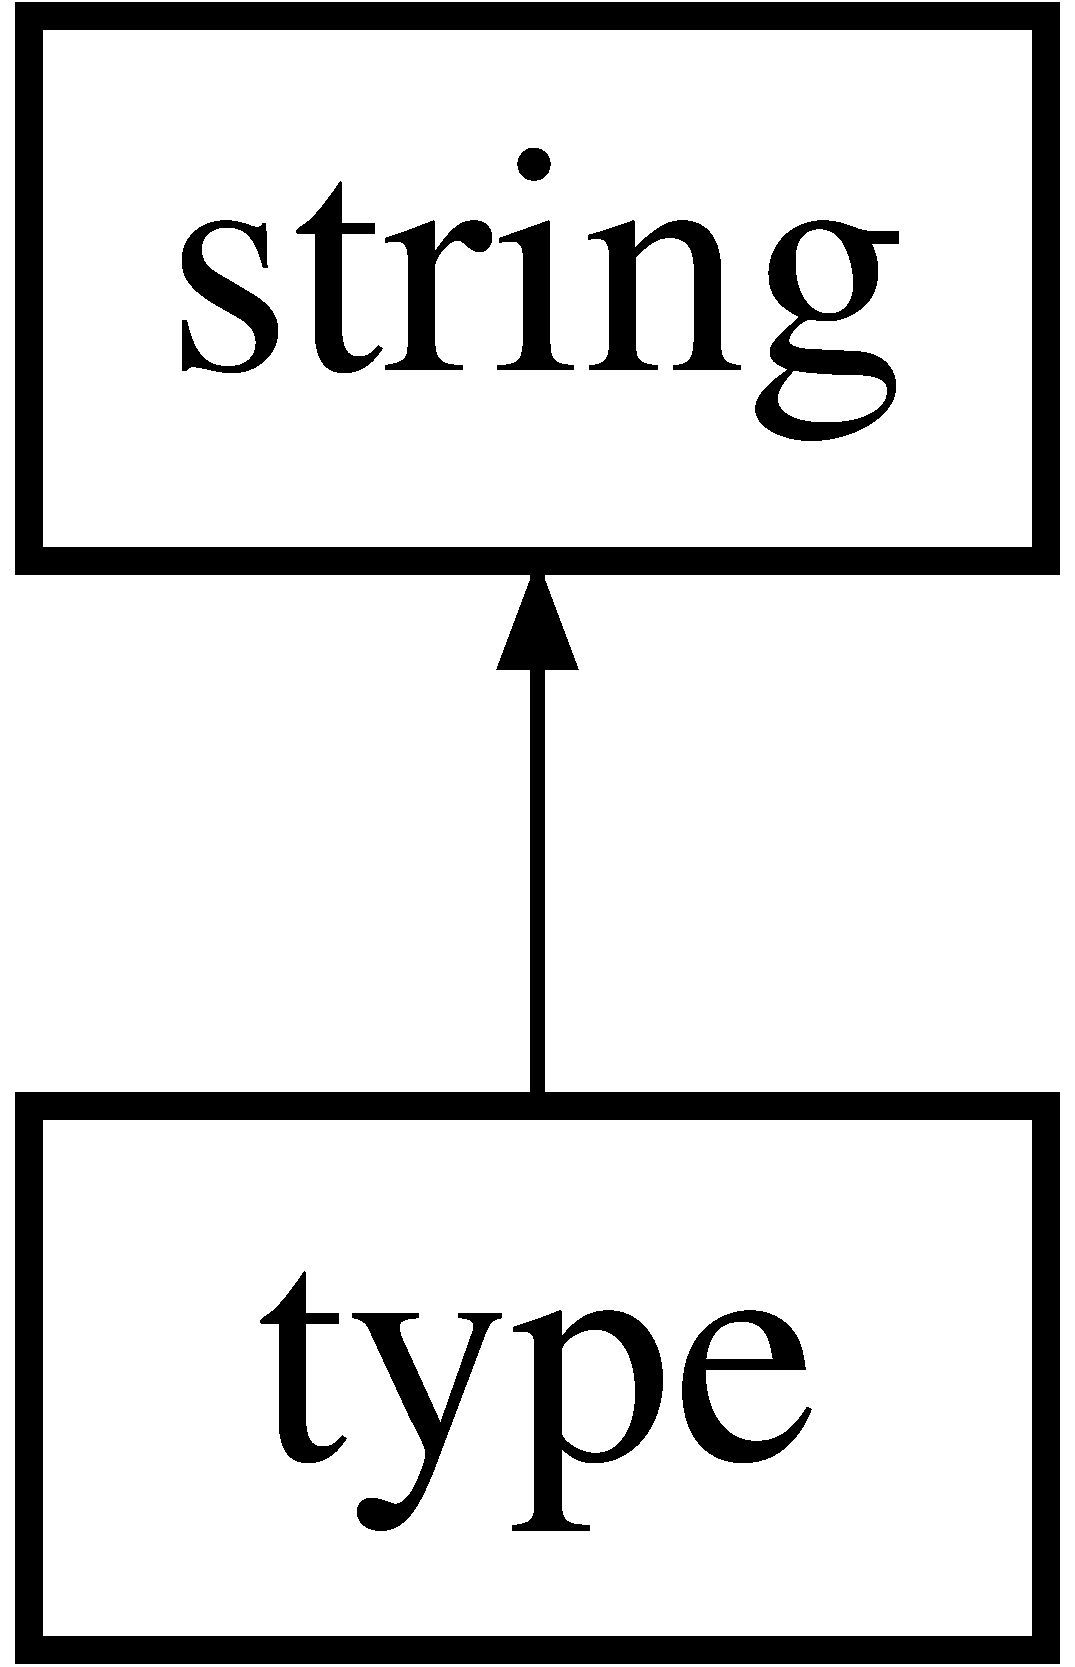
\includegraphics[height=2.000000cm]{classtype}
\end{center}
\end{figure}
\subsection*{Public Types}
\begin{DoxyCompactItemize}
\item 
enum \hyperlink{classtype_a83781d700ce124b4224c316326a5a975}{value} \{ \\*
\hyperlink{classtype_a83781d700ce124b4224c316326a5a975ad559d992c88431b0a1cb90b340929d4e}{Int8}, 
\hyperlink{classtype_a83781d700ce124b4224c316326a5a975a82bbc808c985056ed74b30bcca131fad}{U\+Int8}, 
\hyperlink{classtype_a83781d700ce124b4224c316326a5a975a8d3d044c5da17c4e92e2c61c2f0ea556}{Int16}, 
\hyperlink{classtype_a83781d700ce124b4224c316326a5a975a36b08866238b21675704f38517929e69}{U\+Int16}, 
\\*
\hyperlink{classtype_a83781d700ce124b4224c316326a5a975a62e1ad64aa38ad0b50e1a6bd9b9ae25e}{Int32}, 
\hyperlink{classtype_a83781d700ce124b4224c316326a5a975acfca6c13984dbb7ac515cff88a01826e}{U\+Int32}, 
\hyperlink{classtype_a83781d700ce124b4224c316326a5a975a2cc7bf870db9a3b5e9e580a58b6c1308}{Int64}, 
\hyperlink{classtype_a83781d700ce124b4224c316326a5a975a64538f1914f2fd739bc876253b75fe4c}{U\+Int64}, 
\\*
\hyperlink{classtype_a83781d700ce124b4224c316326a5a975a1b5e448b6fc2bafbc9b5f8e4cc582834}{Float32}, 
\hyperlink{classtype_a83781d700ce124b4224c316326a5a975a72818204734582235e144a1e64563947}{Float64}
 \}
\begin{DoxyCompactList}\small\item\em Underlying enum type. \end{DoxyCompactList}\end{DoxyCompactItemize}
\subsection*{Public Member Functions}
\begin{DoxyCompactItemize}
\item 
\hyperlink{classtype_aed51d13ee609d224084c6cf0a9903f99}{type} (\hyperlink{classtype_a83781d700ce124b4224c316326a5a975}{value} v)
\begin{DoxyCompactList}\small\item\em Create an instance from the underlying enum value. \end{DoxyCompactList}\item 
\hyperlink{classtype_aa5e87da016a56579ba0fc72de17517a5}{type} (const char $\ast$v)
\begin{DoxyCompactList}\small\item\em Create an instance from a C string. \end{DoxyCompactList}\item 
\hyperlink{classtype_ae83bd8bffd0b7251dd664efe908511e7}{type} (const \+::std\+::string \&v)
\begin{DoxyCompactList}\small\item\em Create an instance from a string. \end{DoxyCompactList}\item 
\hyperlink{classtype_a9638b8e282f51d97c9e4e8d703e1f89c}{type} (const \+::\hyperlink{namespacexml__schema_aefbaf353f9a0043af46d23d9040ef268}{xml\+\_\+schema\+::string} \&v)
\begin{DoxyCompactList}\small\item\em Create an instance from the base value. \end{DoxyCompactList}\item 
\hyperlink{classtype_aae224adcb4348cedbe90f4af5dcf1353}{type} (const \+::xercesc\+::\+D\+O\+M\+Element \&e,\+::\hyperlink{namespacexml__schema_a8d981c127a1f5106d04ad5853e707361}{xml\+\_\+schema\+::flags} f=0,\+::\hyperlink{namespacexml__schema_a395f5179c5fc4643909d66e9ff28d8ca}{xml\+\_\+schema\+::container} $\ast$c=0)
\begin{DoxyCompactList}\small\item\em Create an instance from a D\+O\+M element. \end{DoxyCompactList}\item 
\hyperlink{classtype_a7018bbc02d3c782aed64822b87dda220}{type} (const \+::xercesc\+::\+D\+O\+M\+Attr \&a,\+::\hyperlink{namespacexml__schema_a8d981c127a1f5106d04ad5853e707361}{xml\+\_\+schema\+::flags} f=0,\+::\hyperlink{namespacexml__schema_a395f5179c5fc4643909d66e9ff28d8ca}{xml\+\_\+schema\+::container} $\ast$c=0)
\begin{DoxyCompactList}\small\item\em Create an instance from a D\+O\+M attribute. \end{DoxyCompactList}\item 
\hyperlink{classtype_ac6751e8c63b52e22f73a1ab24d50a082}{type} (const \+::std\+::string \&s, const \+::xercesc\+::\+D\+O\+M\+Element $\ast$e,\+::\hyperlink{namespacexml__schema_a8d981c127a1f5106d04ad5853e707361}{xml\+\_\+schema\+::flags} f=0,\+::\hyperlink{namespacexml__schema_a395f5179c5fc4643909d66e9ff28d8ca}{xml\+\_\+schema\+::container} $\ast$c=0)
\begin{DoxyCompactList}\small\item\em Create an instance from a string fragment. \end{DoxyCompactList}\item 
\hyperlink{classtype_aa5eaba8747f76ddbccbb88f68e3311fe}{type} (const \hyperlink{classtype}{type} \&x,\+::\hyperlink{namespacexml__schema_a8d981c127a1f5106d04ad5853e707361}{xml\+\_\+schema\+::flags} f=0,\+::\hyperlink{namespacexml__schema_a395f5179c5fc4643909d66e9ff28d8ca}{xml\+\_\+schema\+::container} $\ast$c=0)
\begin{DoxyCompactList}\small\item\em Copy constructor. \end{DoxyCompactList}\item 
virtual \hyperlink{classtype}{type} $\ast$ \hyperlink{classtype_afebbdc11bbf07de7ab79f148e9cd88b6}{\+\_\+clone} (\+::\hyperlink{namespacexml__schema_a8d981c127a1f5106d04ad5853e707361}{xml\+\_\+schema\+::flags} f=0,\+::\hyperlink{namespacexml__schema_a395f5179c5fc4643909d66e9ff28d8ca}{xml\+\_\+schema\+::container} $\ast$c=0) const 
\begin{DoxyCompactList}\small\item\em Copy the instance polymorphically. \end{DoxyCompactList}\item 
\hyperlink{classtype}{type} \& \hyperlink{classtype_af55f6d7e02cf92b839d842a58e2911ed}{operator=} (\hyperlink{classtype_a83781d700ce124b4224c316326a5a975}{value} v)
\begin{DoxyCompactList}\small\item\em Assign the underlying enum value. \end{DoxyCompactList}\item 
virtual \hyperlink{classtype_a5bfa60d90029d683cb4e46de45460246}{operator value} () const 
\begin{DoxyCompactList}\small\item\em Implicit conversion operator to the underlying enum value. \end{DoxyCompactList}\end{DoxyCompactItemize}


\subsection{Detailed Description}
Enumeration class corresponding to the type schema type. 

\subsection{Member Enumeration Documentation}
\hypertarget{classtype_a83781d700ce124b4224c316326a5a975}{}\index{type@{type}!value@{value}}
\index{value@{value}!type@{type}}
\subsubsection[{value}]{\setlength{\rightskip}{0pt plus 5cm}enum {\bf type\+::value}}\label{classtype_a83781d700ce124b4224c316326a5a975}


Underlying enum type. 

\begin{Desc}
\item[Enumerator]\par
\begin{description}
\index{Int8@{Int8}!type@{type}}\index{type@{type}!Int8@{Int8}}\item[{\em 
\hypertarget{classtype_a83781d700ce124b4224c316326a5a975ad559d992c88431b0a1cb90b340929d4e}{}Int8\label{classtype_a83781d700ce124b4224c316326a5a975ad559d992c88431b0a1cb90b340929d4e}
}]\index{U\+Int8@{U\+Int8}!type@{type}}\index{type@{type}!U\+Int8@{U\+Int8}}\item[{\em 
\hypertarget{classtype_a83781d700ce124b4224c316326a5a975a82bbc808c985056ed74b30bcca131fad}{}U\+Int8\label{classtype_a83781d700ce124b4224c316326a5a975a82bbc808c985056ed74b30bcca131fad}
}]\index{Int16@{Int16}!type@{type}}\index{type@{type}!Int16@{Int16}}\item[{\em 
\hypertarget{classtype_a83781d700ce124b4224c316326a5a975a8d3d044c5da17c4e92e2c61c2f0ea556}{}Int16\label{classtype_a83781d700ce124b4224c316326a5a975a8d3d044c5da17c4e92e2c61c2f0ea556}
}]\index{U\+Int16@{U\+Int16}!type@{type}}\index{type@{type}!U\+Int16@{U\+Int16}}\item[{\em 
\hypertarget{classtype_a83781d700ce124b4224c316326a5a975a36b08866238b21675704f38517929e69}{}U\+Int16\label{classtype_a83781d700ce124b4224c316326a5a975a36b08866238b21675704f38517929e69}
}]\index{Int32@{Int32}!type@{type}}\index{type@{type}!Int32@{Int32}}\item[{\em 
\hypertarget{classtype_a83781d700ce124b4224c316326a5a975a62e1ad64aa38ad0b50e1a6bd9b9ae25e}{}Int32\label{classtype_a83781d700ce124b4224c316326a5a975a62e1ad64aa38ad0b50e1a6bd9b9ae25e}
}]\index{U\+Int32@{U\+Int32}!type@{type}}\index{type@{type}!U\+Int32@{U\+Int32}}\item[{\em 
\hypertarget{classtype_a83781d700ce124b4224c316326a5a975acfca6c13984dbb7ac515cff88a01826e}{}U\+Int32\label{classtype_a83781d700ce124b4224c316326a5a975acfca6c13984dbb7ac515cff88a01826e}
}]\index{Int64@{Int64}!type@{type}}\index{type@{type}!Int64@{Int64}}\item[{\em 
\hypertarget{classtype_a83781d700ce124b4224c316326a5a975a2cc7bf870db9a3b5e9e580a58b6c1308}{}Int64\label{classtype_a83781d700ce124b4224c316326a5a975a2cc7bf870db9a3b5e9e580a58b6c1308}
}]\index{U\+Int64@{U\+Int64}!type@{type}}\index{type@{type}!U\+Int64@{U\+Int64}}\item[{\em 
\hypertarget{classtype_a83781d700ce124b4224c316326a5a975a64538f1914f2fd739bc876253b75fe4c}{}U\+Int64\label{classtype_a83781d700ce124b4224c316326a5a975a64538f1914f2fd739bc876253b75fe4c}
}]\index{Float32@{Float32}!type@{type}}\index{type@{type}!Float32@{Float32}}\item[{\em 
\hypertarget{classtype_a83781d700ce124b4224c316326a5a975a1b5e448b6fc2bafbc9b5f8e4cc582834}{}Float32\label{classtype_a83781d700ce124b4224c316326a5a975a1b5e448b6fc2bafbc9b5f8e4cc582834}
}]\index{Float64@{Float64}!type@{type}}\index{type@{type}!Float64@{Float64}}\item[{\em 
\hypertarget{classtype_a83781d700ce124b4224c316326a5a975a72818204734582235e144a1e64563947}{}Float64\label{classtype_a83781d700ce124b4224c316326a5a975a72818204734582235e144a1e64563947}
}]\end{description}
\end{Desc}


\subsection{Constructor \& Destructor Documentation}
\hypertarget{classtype_aed51d13ee609d224084c6cf0a9903f99}{}\index{type@{type}!type@{type}}
\index{type@{type}!type@{type}}
\subsubsection[{type}]{\setlength{\rightskip}{0pt plus 5cm}type\+::type (
\begin{DoxyParamCaption}
\item[{{\bf value}}]{v}
\end{DoxyParamCaption}
)}\label{classtype_aed51d13ee609d224084c6cf0a9903f99}


Create an instance from the underlying enum value. 


\begin{DoxyParams}{Parameters}
{\em v} & A enum value. \\
\hline
\end{DoxyParams}
\hypertarget{classtype_aa5e87da016a56579ba0fc72de17517a5}{}\index{type@{type}!type@{type}}
\index{type@{type}!type@{type}}
\subsubsection[{type}]{\setlength{\rightskip}{0pt plus 5cm}type\+::type (
\begin{DoxyParamCaption}
\item[{const char $\ast$}]{v}
\end{DoxyParamCaption}
)}\label{classtype_aa5e87da016a56579ba0fc72de17517a5}


Create an instance from a C string. 


\begin{DoxyParams}{Parameters}
{\em v} & A string value. \\
\hline
\end{DoxyParams}
\hypertarget{classtype_ae83bd8bffd0b7251dd664efe908511e7}{}\index{type@{type}!type@{type}}
\index{type@{type}!type@{type}}
\subsubsection[{type}]{\setlength{\rightskip}{0pt plus 5cm}type\+::type (
\begin{DoxyParamCaption}
\item[{const \+::std\+::string \&}]{v}
\end{DoxyParamCaption}
)}\label{classtype_ae83bd8bffd0b7251dd664efe908511e7}


Create an instance from a string. 


\begin{DoxyParams}{Parameters}
{\em v} & A string value. \\
\hline
\end{DoxyParams}
\hypertarget{classtype_a9638b8e282f51d97c9e4e8d703e1f89c}{}\index{type@{type}!type@{type}}
\index{type@{type}!type@{type}}
\subsubsection[{type}]{\setlength{\rightskip}{0pt plus 5cm}type\+::type (
\begin{DoxyParamCaption}
\item[{const \+::{\bf xml\+\_\+schema\+::string} \&}]{v}
\end{DoxyParamCaption}
)}\label{classtype_a9638b8e282f51d97c9e4e8d703e1f89c}


Create an instance from the base value. 


\begin{DoxyParams}{Parameters}
{\em v} & A base value. \\
\hline
\end{DoxyParams}
\hypertarget{classtype_aae224adcb4348cedbe90f4af5dcf1353}{}\index{type@{type}!type@{type}}
\index{type@{type}!type@{type}}
\subsubsection[{type}]{\setlength{\rightskip}{0pt plus 5cm}type\+::type (
\begin{DoxyParamCaption}
\item[{const \+::xercesc\+::\+D\+O\+M\+Element \&}]{e, }
\item[{\+::{\bf xml\+\_\+schema\+::flags}}]{f = {\ttfamily 0}, }
\item[{\+::{\bf xml\+\_\+schema\+::container} $\ast$}]{c = {\ttfamily 0}}
\end{DoxyParamCaption}
)}\label{classtype_aae224adcb4348cedbe90f4af5dcf1353}


Create an instance from a D\+O\+M element. 


\begin{DoxyParams}{Parameters}
{\em e} & A D\+O\+M element to extract the data from. \\
\hline
{\em f} & Flags to create the new instance with. \\
\hline
{\em c} & A pointer to the object that will contain the new instance. \\
\hline
\end{DoxyParams}
\hypertarget{classtype_a7018bbc02d3c782aed64822b87dda220}{}\index{type@{type}!type@{type}}
\index{type@{type}!type@{type}}
\subsubsection[{type}]{\setlength{\rightskip}{0pt plus 5cm}type\+::type (
\begin{DoxyParamCaption}
\item[{const \+::xercesc\+::\+D\+O\+M\+Attr \&}]{a, }
\item[{\+::{\bf xml\+\_\+schema\+::flags}}]{f = {\ttfamily 0}, }
\item[{\+::{\bf xml\+\_\+schema\+::container} $\ast$}]{c = {\ttfamily 0}}
\end{DoxyParamCaption}
)}\label{classtype_a7018bbc02d3c782aed64822b87dda220}


Create an instance from a D\+O\+M attribute. 


\begin{DoxyParams}{Parameters}
{\em a} & A D\+O\+M attribute to extract the data from. \\
\hline
{\em f} & Flags to create the new instance with. \\
\hline
{\em c} & A pointer to the object that will contain the new instance. \\
\hline
\end{DoxyParams}
\hypertarget{classtype_ac6751e8c63b52e22f73a1ab24d50a082}{}\index{type@{type}!type@{type}}
\index{type@{type}!type@{type}}
\subsubsection[{type}]{\setlength{\rightskip}{0pt plus 5cm}type\+::type (
\begin{DoxyParamCaption}
\item[{const \+::std\+::string \&}]{s, }
\item[{const \+::xercesc\+::\+D\+O\+M\+Element $\ast$}]{e, }
\item[{\+::{\bf xml\+\_\+schema\+::flags}}]{f = {\ttfamily 0}, }
\item[{\+::{\bf xml\+\_\+schema\+::container} $\ast$}]{c = {\ttfamily 0}}
\end{DoxyParamCaption}
)}\label{classtype_ac6751e8c63b52e22f73a1ab24d50a082}


Create an instance from a string fragment. 


\begin{DoxyParams}{Parameters}
{\em s} & A string fragment to extract the data from. \\
\hline
{\em e} & A pointer to D\+O\+M element containing the string fragment. \\
\hline
{\em f} & Flags to create the new instance with. \\
\hline
{\em c} & A pointer to the object that will contain the new instance. \\
\hline
\end{DoxyParams}
\hypertarget{classtype_aa5eaba8747f76ddbccbb88f68e3311fe}{}\index{type@{type}!type@{type}}
\index{type@{type}!type@{type}}
\subsubsection[{type}]{\setlength{\rightskip}{0pt plus 5cm}type\+::type (
\begin{DoxyParamCaption}
\item[{const {\bf type} \&}]{x, }
\item[{\+::{\bf xml\+\_\+schema\+::flags}}]{f = {\ttfamily 0}, }
\item[{\+::{\bf xml\+\_\+schema\+::container} $\ast$}]{c = {\ttfamily 0}}
\end{DoxyParamCaption}
)}\label{classtype_aa5eaba8747f76ddbccbb88f68e3311fe}


Copy constructor. 


\begin{DoxyParams}{Parameters}
{\em x} & An instance to make a copy of. \\
\hline
{\em f} & Flags to create the copy with. \\
\hline
{\em c} & A pointer to the object that will contain the copy.\\
\hline
\end{DoxyParams}
For polymorphic object models use the {\ttfamily \+\_\+clone} function instead. 

\subsection{Member Function Documentation}
\hypertarget{classtype_afebbdc11bbf07de7ab79f148e9cd88b6}{}\index{type@{type}!\+\_\+clone@{\+\_\+clone}}
\index{\+\_\+clone@{\+\_\+clone}!type@{type}}
\subsubsection[{\+\_\+clone}]{\setlength{\rightskip}{0pt plus 5cm}{\bf type} $\ast$ type\+::\+\_\+clone (
\begin{DoxyParamCaption}
\item[{\+::{\bf xml\+\_\+schema\+::flags}}]{f = {\ttfamily 0}, }
\item[{\+::{\bf xml\+\_\+schema\+::container} $\ast$}]{c = {\ttfamily 0}}
\end{DoxyParamCaption}
) const\hspace{0.3cm}{\ttfamily [virtual]}}\label{classtype_afebbdc11bbf07de7ab79f148e9cd88b6}


Copy the instance polymorphically. 


\begin{DoxyParams}{Parameters}
{\em f} & Flags to create the copy with. \\
\hline
{\em c} & A pointer to the object that will contain the copy. \\
\hline
\end{DoxyParams}
\begin{DoxyReturn}{Returns}
A pointer to the dynamically allocated copy.
\end{DoxyReturn}
This function ensures that the dynamic type of the instance is used for copying and should be used for polymorphic object models instead of the copy constructor. \hypertarget{classtype_a5bfa60d90029d683cb4e46de45460246}{}\index{type@{type}!operator value@{operator value}}
\index{operator value@{operator value}!type@{type}}
\subsubsection[{operator value}]{\setlength{\rightskip}{0pt plus 5cm}virtual type\+::operator {\bf value} (
\begin{DoxyParamCaption}
{}
\end{DoxyParamCaption}
) const\hspace{0.3cm}{\ttfamily [inline]}, {\ttfamily [virtual]}}\label{classtype_a5bfa60d90029d683cb4e46de45460246}


Implicit conversion operator to the underlying enum value. 

\begin{DoxyReturn}{Returns}
A enum value. 
\end{DoxyReturn}
\hypertarget{classtype_af55f6d7e02cf92b839d842a58e2911ed}{}\index{type@{type}!operator=@{operator=}}
\index{operator=@{operator=}!type@{type}}
\subsubsection[{operator=}]{\setlength{\rightskip}{0pt plus 5cm}{\bf type} \& type\+::operator= (
\begin{DoxyParamCaption}
\item[{{\bf value}}]{v}
\end{DoxyParamCaption}
)}\label{classtype_af55f6d7e02cf92b839d842a58e2911ed}


Assign the underlying enum value. 


\begin{DoxyParams}{Parameters}
{\em v} & A enum value. \\
\hline
\end{DoxyParams}
\begin{DoxyReturn}{Returns}
A refernce to the instance. 
\end{DoxyReturn}


The documentation for this class was generated from the following files\+:\begin{DoxyCompactItemize}
\item 
src/output\+Writer/\hyperlink{vtk-unstructured_8h}{vtk-\/unstructured.\+h}\item 
src/output\+Writer/\hyperlink{vtk-unstructured_8cpp}{vtk-\/unstructured.\+cpp}\end{DoxyCompactItemize}

\hypertarget{classUnstructuredGrid__t}{}\section{Unstructured\+Grid\+\_\+t Class Reference}
\label{classUnstructuredGrid__t}\index{Unstructured\+Grid\+\_\+t@{Unstructured\+Grid\+\_\+t}}


Class corresponding to the Unstructured\+Grid\+\_\+t schema type.  




{\ttfamily \#include $<$vtk-\/unstructured.\+h$>$}

Inheritance diagram for Unstructured\+Grid\+\_\+t\+:\begin{figure}[H]
\begin{center}
\leavevmode
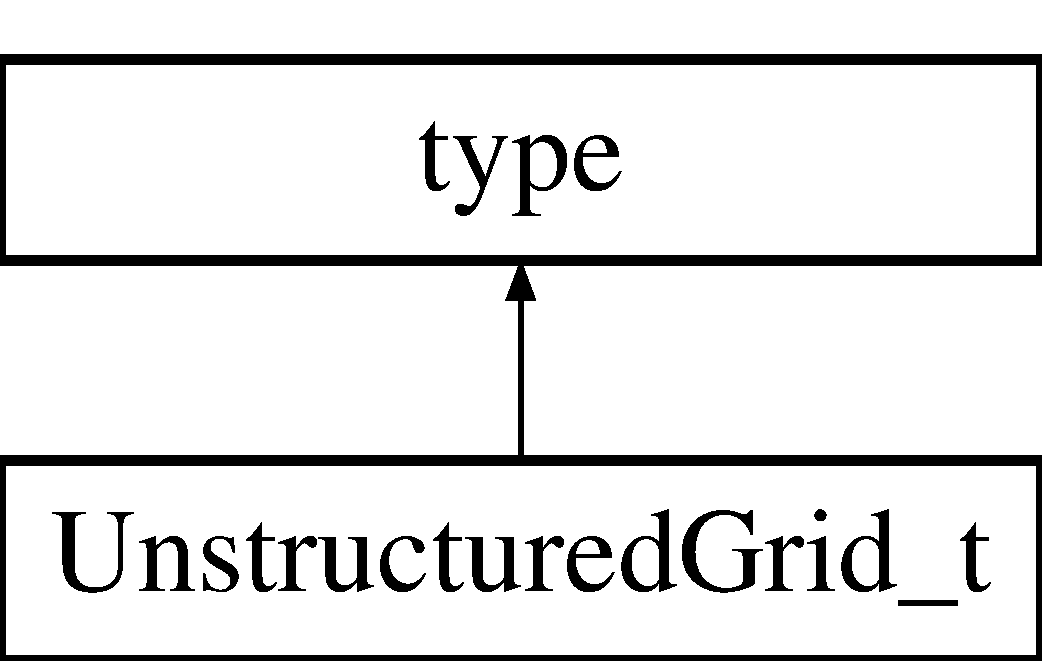
\includegraphics[height=2.000000cm]{classUnstructuredGrid__t}
\end{center}
\end{figure}
\subsection*{Public Member Functions}
\begin{DoxyCompactItemize}
\item 
virtual \hyperlink{classUnstructuredGrid__t_a6fb9239ab1215edd7e7822a66d3af53c}{$\sim$\+Unstructured\+Grid\+\_\+t} ()
\begin{DoxyCompactList}\small\item\em Destructor. \end{DoxyCompactList}\end{DoxyCompactItemize}
\subsection*{Piece}
\label{_amgrpa5d512bf83495b68d0ffa20f79804dfc}%
Accessor and modifier functions for the Piece required element. \begin{DoxyCompactItemize}
\item 
typedef \+::\hyperlink{classPieceUnstructuredGrid__t}{Piece\+Unstructured\+Grid\+\_\+t} \hyperlink{classUnstructuredGrid__t_a559913611314b34f4868027fc91e35bc}{Piece\+\_\+type}
\begin{DoxyCompactList}\small\item\em Element type. \end{DoxyCompactList}\item 
typedef \+::xsd\+::cxx\+::tree\+::traits$<$ \hyperlink{classUnstructuredGrid__t_a559913611314b34f4868027fc91e35bc}{Piece\+\_\+type}, char $>$ \hyperlink{classUnstructuredGrid__t_a8a9bf012c364a5fbb78aac9a319a4dad}{Piece\+\_\+traits}
\begin{DoxyCompactList}\small\item\em Element traits type. \end{DoxyCompactList}\item 
const \hyperlink{classUnstructuredGrid__t_a559913611314b34f4868027fc91e35bc}{Piece\+\_\+type} \& \hyperlink{classUnstructuredGrid__t_a32fdd47d79cfdd2eb071cf674b7cc9ee}{Piece} () const 
\begin{DoxyCompactList}\small\item\em Return a read-\/only (constant) reference to the element. \end{DoxyCompactList}\item 
\hyperlink{classUnstructuredGrid__t_a559913611314b34f4868027fc91e35bc}{Piece\+\_\+type} \& \hyperlink{classUnstructuredGrid__t_a66b7c6fc204fdc78b4611fd132771573}{Piece} ()
\begin{DoxyCompactList}\small\item\em Return a read-\/write reference to the element. \end{DoxyCompactList}\item 
void \hyperlink{classUnstructuredGrid__t_a97ef3f79738631a4265c4fbeb170f04d}{Piece} (const \hyperlink{classUnstructuredGrid__t_a559913611314b34f4868027fc91e35bc}{Piece\+\_\+type} \&x)
\begin{DoxyCompactList}\small\item\em Set the element value. \end{DoxyCompactList}\item 
void \hyperlink{classUnstructuredGrid__t_aadd93b1b259778a8ef49c3d6e5b0be5d}{Piece} (\+::std\+::auto\+\_\+ptr$<$ \hyperlink{classUnstructuredGrid__t_a559913611314b34f4868027fc91e35bc}{Piece\+\_\+type} $>$ p)
\begin{DoxyCompactList}\small\item\em Set the element value without copying. \end{DoxyCompactList}\end{DoxyCompactItemize}
\subsection*{Constructors}
\begin{DoxyCompactItemize}
\item 
\hyperlink{classUnstructuredGrid__t_a00bf6957ea7e3313e2890bd4c02f8981}{Unstructured\+Grid\+\_\+t} (const \hyperlink{classUnstructuredGrid__t_a559913611314b34f4868027fc91e35bc}{Piece\+\_\+type} \&)
\begin{DoxyCompactList}\small\item\em Create an instance from the ultimate base and initializers for required elements and attributes. \end{DoxyCompactList}\item 
\hyperlink{classUnstructuredGrid__t_a528c5e53cac3c45f9e5a2ff37197d1c8}{Unstructured\+Grid\+\_\+t} (\+::std\+::auto\+\_\+ptr$<$ \hyperlink{classUnstructuredGrid__t_a559913611314b34f4868027fc91e35bc}{Piece\+\_\+type} $>$ \&)
\begin{DoxyCompactList}\small\item\em Create an instance from the ultimate base and initializers for required elements and attributes (auto\+\_\+ptr version). \end{DoxyCompactList}\item 
\hyperlink{classUnstructuredGrid__t_ad6fb3d97ad8d9443d53e1152a9fa6004}{Unstructured\+Grid\+\_\+t} (const \+::xercesc\+::\+D\+O\+M\+Element \&e,\+::\hyperlink{namespacexml__schema_a8d981c127a1f5106d04ad5853e707361}{xml\+\_\+schema\+::flags} f=0,\+::\hyperlink{namespacexml__schema_a395f5179c5fc4643909d66e9ff28d8ca}{xml\+\_\+schema\+::container} $\ast$c=0)
\begin{DoxyCompactList}\small\item\em Create an instance from a D\+O\+M element. \end{DoxyCompactList}\item 
\hyperlink{classUnstructuredGrid__t_a893b6debad8369f36a3cdc2aaa22b478}{Unstructured\+Grid\+\_\+t} (const \hyperlink{classUnstructuredGrid__t}{Unstructured\+Grid\+\_\+t} \&x,\+::\hyperlink{namespacexml__schema_a8d981c127a1f5106d04ad5853e707361}{xml\+\_\+schema\+::flags} f=0,\+::\hyperlink{namespacexml__schema_a395f5179c5fc4643909d66e9ff28d8ca}{xml\+\_\+schema\+::container} $\ast$c=0)
\begin{DoxyCompactList}\small\item\em Copy constructor. \end{DoxyCompactList}\item 
virtual \hyperlink{classUnstructuredGrid__t}{Unstructured\+Grid\+\_\+t} $\ast$ \hyperlink{classUnstructuredGrid__t_ae51f374b8650e990f30723bdcf181f2d}{\+\_\+clone} (\+::\hyperlink{namespacexml__schema_a8d981c127a1f5106d04ad5853e707361}{xml\+\_\+schema\+::flags} f=0,\+::\hyperlink{namespacexml__schema_a395f5179c5fc4643909d66e9ff28d8ca}{xml\+\_\+schema\+::container} $\ast$c=0) const 
\begin{DoxyCompactList}\small\item\em Copy the instance polymorphically. \end{DoxyCompactList}\end{DoxyCompactItemize}


\subsection{Detailed Description}
Class corresponding to the Unstructured\+Grid\+\_\+t schema type. 

\subsection{Member Typedef Documentation}
\hypertarget{classUnstructuredGrid__t_a8a9bf012c364a5fbb78aac9a319a4dad}{}\index{Unstructured\+Grid\+\_\+t@{Unstructured\+Grid\+\_\+t}!Piece\+\_\+traits@{Piece\+\_\+traits}}
\index{Piece\+\_\+traits@{Piece\+\_\+traits}!Unstructured\+Grid\+\_\+t@{Unstructured\+Grid\+\_\+t}}
\subsubsection[{Piece\+\_\+traits}]{\setlength{\rightskip}{0pt plus 5cm}typedef \+::xsd\+::cxx\+::tree\+::traits$<$ {\bf Piece\+\_\+type}, char $>$ {\bf Unstructured\+Grid\+\_\+t\+::\+Piece\+\_\+traits}}\label{classUnstructuredGrid__t_a8a9bf012c364a5fbb78aac9a319a4dad}


Element traits type. 

\hypertarget{classUnstructuredGrid__t_a559913611314b34f4868027fc91e35bc}{}\index{Unstructured\+Grid\+\_\+t@{Unstructured\+Grid\+\_\+t}!Piece\+\_\+type@{Piece\+\_\+type}}
\index{Piece\+\_\+type@{Piece\+\_\+type}!Unstructured\+Grid\+\_\+t@{Unstructured\+Grid\+\_\+t}}
\subsubsection[{Piece\+\_\+type}]{\setlength{\rightskip}{0pt plus 5cm}typedef \+::{\bf Piece\+Unstructured\+Grid\+\_\+t} {\bf Unstructured\+Grid\+\_\+t\+::\+Piece\+\_\+type}}\label{classUnstructuredGrid__t_a559913611314b34f4868027fc91e35bc}


Element type. 



\subsection{Constructor \& Destructor Documentation}
\hypertarget{classUnstructuredGrid__t_a00bf6957ea7e3313e2890bd4c02f8981}{}\index{Unstructured\+Grid\+\_\+t@{Unstructured\+Grid\+\_\+t}!Unstructured\+Grid\+\_\+t@{Unstructured\+Grid\+\_\+t}}
\index{Unstructured\+Grid\+\_\+t@{Unstructured\+Grid\+\_\+t}!Unstructured\+Grid\+\_\+t@{Unstructured\+Grid\+\_\+t}}
\subsubsection[{Unstructured\+Grid\+\_\+t}]{\setlength{\rightskip}{0pt plus 5cm}Unstructured\+Grid\+\_\+t\+::\+Unstructured\+Grid\+\_\+t (
\begin{DoxyParamCaption}
\item[{const {\bf Piece\+\_\+type} \&}]{Piece}
\end{DoxyParamCaption}
)}\label{classUnstructuredGrid__t_a00bf6957ea7e3313e2890bd4c02f8981}


Create an instance from the ultimate base and initializers for required elements and attributes. 

\hypertarget{classUnstructuredGrid__t_a528c5e53cac3c45f9e5a2ff37197d1c8}{}\index{Unstructured\+Grid\+\_\+t@{Unstructured\+Grid\+\_\+t}!Unstructured\+Grid\+\_\+t@{Unstructured\+Grid\+\_\+t}}
\index{Unstructured\+Grid\+\_\+t@{Unstructured\+Grid\+\_\+t}!Unstructured\+Grid\+\_\+t@{Unstructured\+Grid\+\_\+t}}
\subsubsection[{Unstructured\+Grid\+\_\+t}]{\setlength{\rightskip}{0pt plus 5cm}Unstructured\+Grid\+\_\+t\+::\+Unstructured\+Grid\+\_\+t (
\begin{DoxyParamCaption}
\item[{\+::std\+::auto\+\_\+ptr$<$ {\bf Piece\+\_\+type} $>$ \&}]{Piece}
\end{DoxyParamCaption}
)}\label{classUnstructuredGrid__t_a528c5e53cac3c45f9e5a2ff37197d1c8}


Create an instance from the ultimate base and initializers for required elements and attributes (auto\+\_\+ptr version). 

This constructor will try to use the passed values directly instead of making copies. \hypertarget{classUnstructuredGrid__t_ad6fb3d97ad8d9443d53e1152a9fa6004}{}\index{Unstructured\+Grid\+\_\+t@{Unstructured\+Grid\+\_\+t}!Unstructured\+Grid\+\_\+t@{Unstructured\+Grid\+\_\+t}}
\index{Unstructured\+Grid\+\_\+t@{Unstructured\+Grid\+\_\+t}!Unstructured\+Grid\+\_\+t@{Unstructured\+Grid\+\_\+t}}
\subsubsection[{Unstructured\+Grid\+\_\+t}]{\setlength{\rightskip}{0pt plus 5cm}Unstructured\+Grid\+\_\+t\+::\+Unstructured\+Grid\+\_\+t (
\begin{DoxyParamCaption}
\item[{const \+::xercesc\+::\+D\+O\+M\+Element \&}]{e, }
\item[{\+::{\bf xml\+\_\+schema\+::flags}}]{f = {\ttfamily 0}, }
\item[{\+::{\bf xml\+\_\+schema\+::container} $\ast$}]{c = {\ttfamily 0}}
\end{DoxyParamCaption}
)}\label{classUnstructuredGrid__t_ad6fb3d97ad8d9443d53e1152a9fa6004}


Create an instance from a D\+O\+M element. 


\begin{DoxyParams}{Parameters}
{\em e} & A D\+O\+M element to extract the data from. \\
\hline
{\em f} & Flags to create the new instance with. \\
\hline
{\em c} & A pointer to the object that will contain the new instance. \\
\hline
\end{DoxyParams}
\hypertarget{classUnstructuredGrid__t_a893b6debad8369f36a3cdc2aaa22b478}{}\index{Unstructured\+Grid\+\_\+t@{Unstructured\+Grid\+\_\+t}!Unstructured\+Grid\+\_\+t@{Unstructured\+Grid\+\_\+t}}
\index{Unstructured\+Grid\+\_\+t@{Unstructured\+Grid\+\_\+t}!Unstructured\+Grid\+\_\+t@{Unstructured\+Grid\+\_\+t}}
\subsubsection[{Unstructured\+Grid\+\_\+t}]{\setlength{\rightskip}{0pt plus 5cm}Unstructured\+Grid\+\_\+t\+::\+Unstructured\+Grid\+\_\+t (
\begin{DoxyParamCaption}
\item[{const {\bf Unstructured\+Grid\+\_\+t} \&}]{x, }
\item[{\+::{\bf xml\+\_\+schema\+::flags}}]{f = {\ttfamily 0}, }
\item[{\+::{\bf xml\+\_\+schema\+::container} $\ast$}]{c = {\ttfamily 0}}
\end{DoxyParamCaption}
)}\label{classUnstructuredGrid__t_a893b6debad8369f36a3cdc2aaa22b478}


Copy constructor. 


\begin{DoxyParams}{Parameters}
{\em x} & An instance to make a copy of. \\
\hline
{\em f} & Flags to create the copy with. \\
\hline
{\em c} & A pointer to the object that will contain the copy.\\
\hline
\end{DoxyParams}
For polymorphic object models use the {\ttfamily \+\_\+clone} function instead. \hypertarget{classUnstructuredGrid__t_a6fb9239ab1215edd7e7822a66d3af53c}{}\index{Unstructured\+Grid\+\_\+t@{Unstructured\+Grid\+\_\+t}!````~Unstructured\+Grid\+\_\+t@{$\sim$\+Unstructured\+Grid\+\_\+t}}
\index{````~Unstructured\+Grid\+\_\+t@{$\sim$\+Unstructured\+Grid\+\_\+t}!Unstructured\+Grid\+\_\+t@{Unstructured\+Grid\+\_\+t}}
\subsubsection[{$\sim$\+Unstructured\+Grid\+\_\+t}]{\setlength{\rightskip}{0pt plus 5cm}Unstructured\+Grid\+\_\+t\+::$\sim$\+Unstructured\+Grid\+\_\+t (
\begin{DoxyParamCaption}
{}
\end{DoxyParamCaption}
)\hspace{0.3cm}{\ttfamily [virtual]}}\label{classUnstructuredGrid__t_a6fb9239ab1215edd7e7822a66d3af53c}


Destructor. 



\subsection{Member Function Documentation}
\hypertarget{classUnstructuredGrid__t_ae51f374b8650e990f30723bdcf181f2d}{}\index{Unstructured\+Grid\+\_\+t@{Unstructured\+Grid\+\_\+t}!\+\_\+clone@{\+\_\+clone}}
\index{\+\_\+clone@{\+\_\+clone}!Unstructured\+Grid\+\_\+t@{Unstructured\+Grid\+\_\+t}}
\subsubsection[{\+\_\+clone}]{\setlength{\rightskip}{0pt plus 5cm}{\bf Unstructured\+Grid\+\_\+t} $\ast$ Unstructured\+Grid\+\_\+t\+::\+\_\+clone (
\begin{DoxyParamCaption}
\item[{\+::{\bf xml\+\_\+schema\+::flags}}]{f = {\ttfamily 0}, }
\item[{\+::{\bf xml\+\_\+schema\+::container} $\ast$}]{c = {\ttfamily 0}}
\end{DoxyParamCaption}
) const\hspace{0.3cm}{\ttfamily [virtual]}}\label{classUnstructuredGrid__t_ae51f374b8650e990f30723bdcf181f2d}


Copy the instance polymorphically. 


\begin{DoxyParams}{Parameters}
{\em f} & Flags to create the copy with. \\
\hline
{\em c} & A pointer to the object that will contain the copy. \\
\hline
\end{DoxyParams}
\begin{DoxyReturn}{Returns}
A pointer to the dynamically allocated copy.
\end{DoxyReturn}
This function ensures that the dynamic type of the instance is used for copying and should be used for polymorphic object models instead of the copy constructor. \hypertarget{classUnstructuredGrid__t_a32fdd47d79cfdd2eb071cf674b7cc9ee}{}\index{Unstructured\+Grid\+\_\+t@{Unstructured\+Grid\+\_\+t}!Piece@{Piece}}
\index{Piece@{Piece}!Unstructured\+Grid\+\_\+t@{Unstructured\+Grid\+\_\+t}}
\subsubsection[{Piece}]{\setlength{\rightskip}{0pt plus 5cm}const {\bf Unstructured\+Grid\+\_\+t\+::\+Piece\+\_\+type} \& Unstructured\+Grid\+\_\+t\+::\+Piece (
\begin{DoxyParamCaption}
{}
\end{DoxyParamCaption}
) const}\label{classUnstructuredGrid__t_a32fdd47d79cfdd2eb071cf674b7cc9ee}


Return a read-\/only (constant) reference to the element. 

\begin{DoxyReturn}{Returns}
A constant reference to the element. 
\end{DoxyReturn}
\hypertarget{classUnstructuredGrid__t_a66b7c6fc204fdc78b4611fd132771573}{}\index{Unstructured\+Grid\+\_\+t@{Unstructured\+Grid\+\_\+t}!Piece@{Piece}}
\index{Piece@{Piece}!Unstructured\+Grid\+\_\+t@{Unstructured\+Grid\+\_\+t}}
\subsubsection[{Piece}]{\setlength{\rightskip}{0pt plus 5cm}{\bf Unstructured\+Grid\+\_\+t\+::\+Piece\+\_\+type} \& Unstructured\+Grid\+\_\+t\+::\+Piece (
\begin{DoxyParamCaption}
{}
\end{DoxyParamCaption}
)}\label{classUnstructuredGrid__t_a66b7c6fc204fdc78b4611fd132771573}


Return a read-\/write reference to the element. 

\begin{DoxyReturn}{Returns}
A reference to the element. 
\end{DoxyReturn}
\hypertarget{classUnstructuredGrid__t_a97ef3f79738631a4265c4fbeb170f04d}{}\index{Unstructured\+Grid\+\_\+t@{Unstructured\+Grid\+\_\+t}!Piece@{Piece}}
\index{Piece@{Piece}!Unstructured\+Grid\+\_\+t@{Unstructured\+Grid\+\_\+t}}
\subsubsection[{Piece}]{\setlength{\rightskip}{0pt plus 5cm}void Unstructured\+Grid\+\_\+t\+::\+Piece (
\begin{DoxyParamCaption}
\item[{const {\bf Piece\+\_\+type} \&}]{x}
\end{DoxyParamCaption}
)}\label{classUnstructuredGrid__t_a97ef3f79738631a4265c4fbeb170f04d}


Set the element value. 


\begin{DoxyParams}{Parameters}
{\em x} & A new value to set.\\
\hline
\end{DoxyParams}
This function makes a copy of its argument and sets it as the new value of the element. \hypertarget{classUnstructuredGrid__t_aadd93b1b259778a8ef49c3d6e5b0be5d}{}\index{Unstructured\+Grid\+\_\+t@{Unstructured\+Grid\+\_\+t}!Piece@{Piece}}
\index{Piece@{Piece}!Unstructured\+Grid\+\_\+t@{Unstructured\+Grid\+\_\+t}}
\subsubsection[{Piece}]{\setlength{\rightskip}{0pt plus 5cm}void Unstructured\+Grid\+\_\+t\+::\+Piece (
\begin{DoxyParamCaption}
\item[{\+::std\+::auto\+\_\+ptr$<$ {\bf Piece\+\_\+type} $>$}]{p}
\end{DoxyParamCaption}
)}\label{classUnstructuredGrid__t_aadd93b1b259778a8ef49c3d6e5b0be5d}


Set the element value without copying. 


\begin{DoxyParams}{Parameters}
{\em p} & A new value to use.\\
\hline
\end{DoxyParams}
This function will try to use the passed value directly instead of making a copy. 

The documentation for this class was generated from the following files\+:\begin{DoxyCompactItemize}
\item 
src/output\+Writer/\hyperlink{vtk-unstructured_8h}{vtk-\/unstructured.\+h}\item 
src/output\+Writer/\hyperlink{vtk-unstructured_8cpp}{vtk-\/unstructured.\+cpp}\end{DoxyCompactItemize}

\hypertarget{classutils_1_1Vector}{}\section{utils\+:\+:Vector$<$ type, length $>$ Class Template Reference}
\label{classutils_1_1Vector}\index{utils\+::\+Vector$<$ type, length $>$@{utils\+::\+Vector$<$ type, length $>$}}


{\ttfamily \#include $<$Vector.\+h$>$}

\subsection*{Public Member Functions}
\begin{DoxyCompactItemize}
\item 
\hyperlink{classutils_1_1Vector_a71b42b489a54eb7eae82cff54fae0e12}{Vector} ()
\item 
\hyperlink{classutils_1_1Vector_a5f7d3385f6db28e1376d16e46f1a485f}{Vector} (\hyperlink{classtype}{type} arg)
\item 
\hyperlink{classutils_1_1Vector_a61a6f07c23829b70273ab4578bbb2332}{Vector} (\hyperlink{classtype}{type} args\mbox{[}length\mbox{]})
\item 
\hyperlink{classutils_1_1Vector_abb684db142444c4b19e6cd854db1a0d8}{Vector} (const \hyperlink{classutils_1_1Vector}{Vector} \&other)
\item 
\hyperlink{classutils_1_1Vector}{Vector} \hyperlink{classutils_1_1Vector_aeb0edeaa6b74a48839892e16623b0949}{operator+} (const \hyperlink{classutils_1_1Vector}{Vector} \&rhs) const 
\item 
\hyperlink{classutils_1_1Vector}{Vector} \hyperlink{classutils_1_1Vector_ad6e42a80810a58993f39e1d876eb5716}{operator-\/} (const \hyperlink{classutils_1_1Vector}{Vector} \&rhs) const 
\item 
\hyperlink{classutils_1_1Vector}{Vector} \hyperlink{classutils_1_1Vector_a655ed48c281bfb1c87901313eb1896bb}{operator$\ast$} (double scalar) const 
\item 
double \hyperlink{classutils_1_1Vector_aa54009b6a76a8059de0eccbe43524d0c}{L2\+Norm} () const 
\item 
bool \hyperlink{classutils_1_1Vector_a761ff3d4c09a533535452b2a20038782}{equals} (const \hyperlink{classutils_1_1Vector}{Vector} \&rhs) const 
\item 
\hyperlink{classutils_1_1Vector}{Vector} \& \hyperlink{classutils_1_1Vector_a16812f2bf90d9e79b58fd42860c111e7}{operator=} (const \hyperlink{classutils_1_1Vector}{Vector} \&rhs)
\item 
\hyperlink{classutils_1_1Vector}{Vector} \& \hyperlink{classutils_1_1Vector_a5c1cfa1d42abdd9a90b4913892608386}{operator=} (double rhs)
\item 
\hyperlink{classtype}{type} \& \hyperlink{classutils_1_1Vector_a391fe7cbc2441879439fbc191ec4ef03}{operator\mbox{[}$\,$\mbox{]}} (int i)
\item 
const \hyperlink{classtype}{type} \& \hyperlink{classutils_1_1Vector_a3b965c400abae02fcad3751cf4b79309}{operator\mbox{[}$\,$\mbox{]}} (int i) const 
\item 
bool \hyperlink{classutils_1_1Vector_a04ceba4a8df8a367205d1c57063ec3f8}{operator==} (const \hyperlink{classutils_1_1Vector}{Vector} \&rhs) const 
\item 
std\+::string \hyperlink{classutils_1_1Vector_ab71fcfc3a0e80ee4a7d2c0fc76fed9a0}{to\+String} () const 
\end{DoxyCompactItemize}
\subsection*{Private Attributes}
\begin{DoxyCompactItemize}
\item 
\hyperlink{classtype}{type} \hyperlink{classutils_1_1Vector_ab391d67eb8f8563b4dd4b80390a4631a}{content} \mbox{[}length\mbox{]}
\end{DoxyCompactItemize}
\subsection*{Friends}
\begin{DoxyCompactItemize}
\item 
std\+::ostream \& \hyperlink{classutils_1_1Vector_a49b910c983e6c91855b55ab04d401e4f}{operator} (std\+::ostream \&stream, const \hyperlink{classutils_1_1Vector}{Vector} \&v)
\item 
\hyperlink{classutils_1_1Vector}{Vector} \hyperlink{classutils_1_1Vector_a45c43d96a8bbe774870183ff33079584}{operator$\ast$} (double scalar, const \hyperlink{classutils_1_1Vector}{Vector} \&v)
\end{DoxyCompactItemize}


\subsection{Detailed Description}
\subsubsection*{template$<$typename type, int length$>$class utils\+::\+Vector$<$ type, length $>$}

\hyperlink{classutils_1_1Vector}{Vector} class definition 

\subsection{Constructor \& Destructor Documentation}
\hypertarget{classutils_1_1Vector_a71b42b489a54eb7eae82cff54fae0e12}{}\index{utils\+::\+Vector@{utils\+::\+Vector}!Vector@{Vector}}
\index{Vector@{Vector}!utils\+::\+Vector@{utils\+::\+Vector}}
\subsubsection[{Vector}]{\setlength{\rightskip}{0pt plus 5cm}template$<$typename type, int length$>$ {\bf utils\+::\+Vector}$<$ {\bf type}, length $>$\+::{\bf Vector} (
\begin{DoxyParamCaption}
{}
\end{DoxyParamCaption}
)\hspace{0.3cm}{\ttfamily [inline]}}\label{classutils_1_1Vector_a71b42b489a54eb7eae82cff54fae0e12}
\hypertarget{classutils_1_1Vector_a5f7d3385f6db28e1376d16e46f1a485f}{}\index{utils\+::\+Vector@{utils\+::\+Vector}!Vector@{Vector}}
\index{Vector@{Vector}!utils\+::\+Vector@{utils\+::\+Vector}}
\subsubsection[{Vector}]{\setlength{\rightskip}{0pt plus 5cm}template$<$typename type, int length$>$ {\bf utils\+::\+Vector}$<$ {\bf type}, length $>$\+::{\bf Vector} (
\begin{DoxyParamCaption}
\item[{{\bf type}}]{arg}
\end{DoxyParamCaption}
)\hspace{0.3cm}{\ttfamily [inline]}}\label{classutils_1_1Vector_a5f7d3385f6db28e1376d16e46f1a485f}
\hypertarget{classutils_1_1Vector_a61a6f07c23829b70273ab4578bbb2332}{}\index{utils\+::\+Vector@{utils\+::\+Vector}!Vector@{Vector}}
\index{Vector@{Vector}!utils\+::\+Vector@{utils\+::\+Vector}}
\subsubsection[{Vector}]{\setlength{\rightskip}{0pt plus 5cm}template$<$typename type, int length$>$ {\bf utils\+::\+Vector}$<$ {\bf type}, length $>$\+::{\bf Vector} (
\begin{DoxyParamCaption}
\item[{{\bf type}}]{args\mbox{[}length\mbox{]}}
\end{DoxyParamCaption}
)\hspace{0.3cm}{\ttfamily [inline]}}\label{classutils_1_1Vector_a61a6f07c23829b70273ab4578bbb2332}
\hypertarget{classutils_1_1Vector_abb684db142444c4b19e6cd854db1a0d8}{}\index{utils\+::\+Vector@{utils\+::\+Vector}!Vector@{Vector}}
\index{Vector@{Vector}!utils\+::\+Vector@{utils\+::\+Vector}}
\subsubsection[{Vector}]{\setlength{\rightskip}{0pt plus 5cm}template$<$typename type, int length$>$ {\bf utils\+::\+Vector}$<$ {\bf type}, length $>$\+::{\bf Vector} (
\begin{DoxyParamCaption}
\item[{const {\bf Vector}$<$ {\bf type}, length $>$ \&}]{other}
\end{DoxyParamCaption}
)\hspace{0.3cm}{\ttfamily [inline]}}\label{classutils_1_1Vector_abb684db142444c4b19e6cd854db1a0d8}


\subsection{Member Function Documentation}
\hypertarget{classutils_1_1Vector_a761ff3d4c09a533535452b2a20038782}{}\index{utils\+::\+Vector@{utils\+::\+Vector}!equals@{equals}}
\index{equals@{equals}!utils\+::\+Vector@{utils\+::\+Vector}}
\subsubsection[{equals}]{\setlength{\rightskip}{0pt plus 5cm}template$<$typename type, int length$>$ bool {\bf utils\+::\+Vector}$<$ {\bf type}, length $>$\+::equals (
\begin{DoxyParamCaption}
\item[{const {\bf Vector}$<$ {\bf type}, length $>$ \&}]{rhs}
\end{DoxyParamCaption}
) const\hspace{0.3cm}{\ttfamily [inline]}}\label{classutils_1_1Vector_a761ff3d4c09a533535452b2a20038782}
\hypertarget{classutils_1_1Vector_aa54009b6a76a8059de0eccbe43524d0c}{}\index{utils\+::\+Vector@{utils\+::\+Vector}!L2\+Norm@{L2\+Norm}}
\index{L2\+Norm@{L2\+Norm}!utils\+::\+Vector@{utils\+::\+Vector}}
\subsubsection[{L2\+Norm}]{\setlength{\rightskip}{0pt plus 5cm}template$<$typename type, int length$>$ double {\bf utils\+::\+Vector}$<$ {\bf type}, length $>$\+::L2\+Norm (
\begin{DoxyParamCaption}
{}
\end{DoxyParamCaption}
) const\hspace{0.3cm}{\ttfamily [inline]}}\label{classutils_1_1Vector_aa54009b6a76a8059de0eccbe43524d0c}
\hypertarget{classutils_1_1Vector_a655ed48c281bfb1c87901313eb1896bb}{}\index{utils\+::\+Vector@{utils\+::\+Vector}!operator$\ast$@{operator$\ast$}}
\index{operator$\ast$@{operator$\ast$}!utils\+::\+Vector@{utils\+::\+Vector}}
\subsubsection[{operator$\ast$}]{\setlength{\rightskip}{0pt plus 5cm}template$<$typename type, int length$>$ {\bf Vector} {\bf utils\+::\+Vector}$<$ {\bf type}, length $>$\+::{\bf operator}$\ast$ (
\begin{DoxyParamCaption}
\item[{double}]{scalar}
\end{DoxyParamCaption}
) const\hspace{0.3cm}{\ttfamily [inline]}}\label{classutils_1_1Vector_a655ed48c281bfb1c87901313eb1896bb}
\hypertarget{classutils_1_1Vector_aeb0edeaa6b74a48839892e16623b0949}{}\index{utils\+::\+Vector@{utils\+::\+Vector}!operator+@{operator+}}
\index{operator+@{operator+}!utils\+::\+Vector@{utils\+::\+Vector}}
\subsubsection[{operator+}]{\setlength{\rightskip}{0pt plus 5cm}template$<$typename type, int length$>$ {\bf Vector} {\bf utils\+::\+Vector}$<$ {\bf type}, length $>$\+::{\bf operator}+ (
\begin{DoxyParamCaption}
\item[{const {\bf Vector}$<$ {\bf type}, length $>$ \&}]{rhs}
\end{DoxyParamCaption}
) const\hspace{0.3cm}{\ttfamily [inline]}}\label{classutils_1_1Vector_aeb0edeaa6b74a48839892e16623b0949}
\hypertarget{classutils_1_1Vector_ad6e42a80810a58993f39e1d876eb5716}{}\index{utils\+::\+Vector@{utils\+::\+Vector}!operator-\/@{operator-\/}}
\index{operator-\/@{operator-\/}!utils\+::\+Vector@{utils\+::\+Vector}}
\subsubsection[{operator-\/}]{\setlength{\rightskip}{0pt plus 5cm}template$<$typename type, int length$>$ {\bf Vector} {\bf utils\+::\+Vector}$<$ {\bf type}, length $>$\+::{\bf operator}-\/ (
\begin{DoxyParamCaption}
\item[{const {\bf Vector}$<$ {\bf type}, length $>$ \&}]{rhs}
\end{DoxyParamCaption}
) const\hspace{0.3cm}{\ttfamily [inline]}}\label{classutils_1_1Vector_ad6e42a80810a58993f39e1d876eb5716}
\hypertarget{classutils_1_1Vector_a16812f2bf90d9e79b58fd42860c111e7}{}\index{utils\+::\+Vector@{utils\+::\+Vector}!operator=@{operator=}}
\index{operator=@{operator=}!utils\+::\+Vector@{utils\+::\+Vector}}
\subsubsection[{operator=}]{\setlength{\rightskip}{0pt plus 5cm}template$<$typename type, int length$>$ {\bf Vector}\& {\bf utils\+::\+Vector}$<$ {\bf type}, length $>$\+::{\bf operator}= (
\begin{DoxyParamCaption}
\item[{const {\bf Vector}$<$ {\bf type}, length $>$ \&}]{rhs}
\end{DoxyParamCaption}
)\hspace{0.3cm}{\ttfamily [inline]}}\label{classutils_1_1Vector_a16812f2bf90d9e79b58fd42860c111e7}
\hypertarget{classutils_1_1Vector_a5c1cfa1d42abdd9a90b4913892608386}{}\index{utils\+::\+Vector@{utils\+::\+Vector}!operator=@{operator=}}
\index{operator=@{operator=}!utils\+::\+Vector@{utils\+::\+Vector}}
\subsubsection[{operator=}]{\setlength{\rightskip}{0pt plus 5cm}template$<$typename type, int length$>$ {\bf Vector}\& {\bf utils\+::\+Vector}$<$ {\bf type}, length $>$\+::{\bf operator}= (
\begin{DoxyParamCaption}
\item[{double}]{rhs}
\end{DoxyParamCaption}
)\hspace{0.3cm}{\ttfamily [inline]}}\label{classutils_1_1Vector_a5c1cfa1d42abdd9a90b4913892608386}
\hypertarget{classutils_1_1Vector_a04ceba4a8df8a367205d1c57063ec3f8}{}\index{utils\+::\+Vector@{utils\+::\+Vector}!operator==@{operator==}}
\index{operator==@{operator==}!utils\+::\+Vector@{utils\+::\+Vector}}
\subsubsection[{operator==}]{\setlength{\rightskip}{0pt plus 5cm}template$<$typename type, int length$>$ bool {\bf utils\+::\+Vector}$<$ {\bf type}, length $>$\+::{\bf operator}== (
\begin{DoxyParamCaption}
\item[{const {\bf Vector}$<$ {\bf type}, length $>$ \&}]{rhs}
\end{DoxyParamCaption}
) const\hspace{0.3cm}{\ttfamily [inline]}}\label{classutils_1_1Vector_a04ceba4a8df8a367205d1c57063ec3f8}
\hypertarget{classutils_1_1Vector_a391fe7cbc2441879439fbc191ec4ef03}{}\index{utils\+::\+Vector@{utils\+::\+Vector}!operator\mbox{[}$\,$\mbox{]}@{operator[]}}
\index{operator\mbox{[}$\,$\mbox{]}@{operator[]}!utils\+::\+Vector@{utils\+::\+Vector}}
\subsubsection[{operator[]}]{\setlength{\rightskip}{0pt plus 5cm}template$<$typename type, int length$>$ {\bf type}\& {\bf utils\+::\+Vector}$<$ {\bf type}, length $>$\+::{\bf operator}\mbox{[}$\,$\mbox{]} (
\begin{DoxyParamCaption}
\item[{int}]{i}
\end{DoxyParamCaption}
)\hspace{0.3cm}{\ttfamily [inline]}}\label{classutils_1_1Vector_a391fe7cbc2441879439fbc191ec4ef03}
\hypertarget{classutils_1_1Vector_a3b965c400abae02fcad3751cf4b79309}{}\index{utils\+::\+Vector@{utils\+::\+Vector}!operator\mbox{[}$\,$\mbox{]}@{operator[]}}
\index{operator\mbox{[}$\,$\mbox{]}@{operator[]}!utils\+::\+Vector@{utils\+::\+Vector}}
\subsubsection[{operator[]}]{\setlength{\rightskip}{0pt plus 5cm}template$<$typename type, int length$>$ const {\bf type}\& {\bf utils\+::\+Vector}$<$ {\bf type}, length $>$\+::{\bf operator}\mbox{[}$\,$\mbox{]} (
\begin{DoxyParamCaption}
\item[{int}]{i}
\end{DoxyParamCaption}
) const\hspace{0.3cm}{\ttfamily [inline]}}\label{classutils_1_1Vector_a3b965c400abae02fcad3751cf4b79309}
\hypertarget{classutils_1_1Vector_ab71fcfc3a0e80ee4a7d2c0fc76fed9a0}{}\index{utils\+::\+Vector@{utils\+::\+Vector}!to\+String@{to\+String}}
\index{to\+String@{to\+String}!utils\+::\+Vector@{utils\+::\+Vector}}
\subsubsection[{to\+String}]{\setlength{\rightskip}{0pt plus 5cm}template$<$typename type, int length$>$ std\+::string {\bf utils\+::\+Vector}$<$ {\bf type}, length $>$\+::to\+String (
\begin{DoxyParamCaption}
{}
\end{DoxyParamCaption}
) const\hspace{0.3cm}{\ttfamily [inline]}}\label{classutils_1_1Vector_ab71fcfc3a0e80ee4a7d2c0fc76fed9a0}


\subsection{Friends And Related Function Documentation}
\hypertarget{classutils_1_1Vector_a49b910c983e6c91855b55ab04d401e4f}{}\index{utils\+::\+Vector@{utils\+::\+Vector}!operator@{operator}}
\index{operator@{operator}!utils\+::\+Vector@{utils\+::\+Vector}}
\subsubsection[{operator}]{\setlength{\rightskip}{0pt plus 5cm}template$<$typename type, int length$>$ std\+::ostream\& operator (
\begin{DoxyParamCaption}
\item[{std\+::ostream \&}]{stream, }
\item[{const {\bf Vector}$<$ {\bf type}, length $>$ \&}]{v}
\end{DoxyParamCaption}
)\hspace{0.3cm}{\ttfamily [friend]}}\label{classutils_1_1Vector_a49b910c983e6c91855b55ab04d401e4f}
\hypertarget{classutils_1_1Vector_a45c43d96a8bbe774870183ff33079584}{}\index{utils\+::\+Vector@{utils\+::\+Vector}!operator$\ast$@{operator$\ast$}}
\index{operator$\ast$@{operator$\ast$}!utils\+::\+Vector@{utils\+::\+Vector}}
\subsubsection[{operator$\ast$}]{\setlength{\rightskip}{0pt plus 5cm}template$<$typename type, int length$>$ {\bf Vector} {\bf operator}$\ast$ (
\begin{DoxyParamCaption}
\item[{double}]{scalar, }
\item[{const {\bf Vector}$<$ {\bf type}, length $>$ \&}]{v}
\end{DoxyParamCaption}
)\hspace{0.3cm}{\ttfamily [friend]}}\label{classutils_1_1Vector_a45c43d96a8bbe774870183ff33079584}


\subsection{Member Data Documentation}
\hypertarget{classutils_1_1Vector_ab391d67eb8f8563b4dd4b80390a4631a}{}\index{utils\+::\+Vector@{utils\+::\+Vector}!content@{content}}
\index{content@{content}!utils\+::\+Vector@{utils\+::\+Vector}}
\subsubsection[{content}]{\setlength{\rightskip}{0pt plus 5cm}template$<$typename type, int length$>$ {\bf type} {\bf utils\+::\+Vector}$<$ {\bf type}, length $>$\+::content\mbox{[}length\mbox{]}\hspace{0.3cm}{\ttfamily [private]}}\label{classutils_1_1Vector_ab391d67eb8f8563b4dd4b80390a4631a}


The documentation for this class was generated from the following file\+:\begin{DoxyCompactItemize}
\item 
src/utils/\hyperlink{Vector_8h}{Vector.\+h}\end{DoxyCompactItemize}

\hypertarget{classVTKFile__t}{}\section{V\+T\+K\+File\+\_\+t Class Reference}
\label{classVTKFile__t}\index{V\+T\+K\+File\+\_\+t@{V\+T\+K\+File\+\_\+t}}


Class corresponding to the V\+T\+K\+File\+\_\+t schema type.  




{\ttfamily \#include $<$vtk-\/unstructured.\+h$>$}

Inheritance diagram for V\+T\+K\+File\+\_\+t\+:\begin{figure}[H]
\begin{center}
\leavevmode
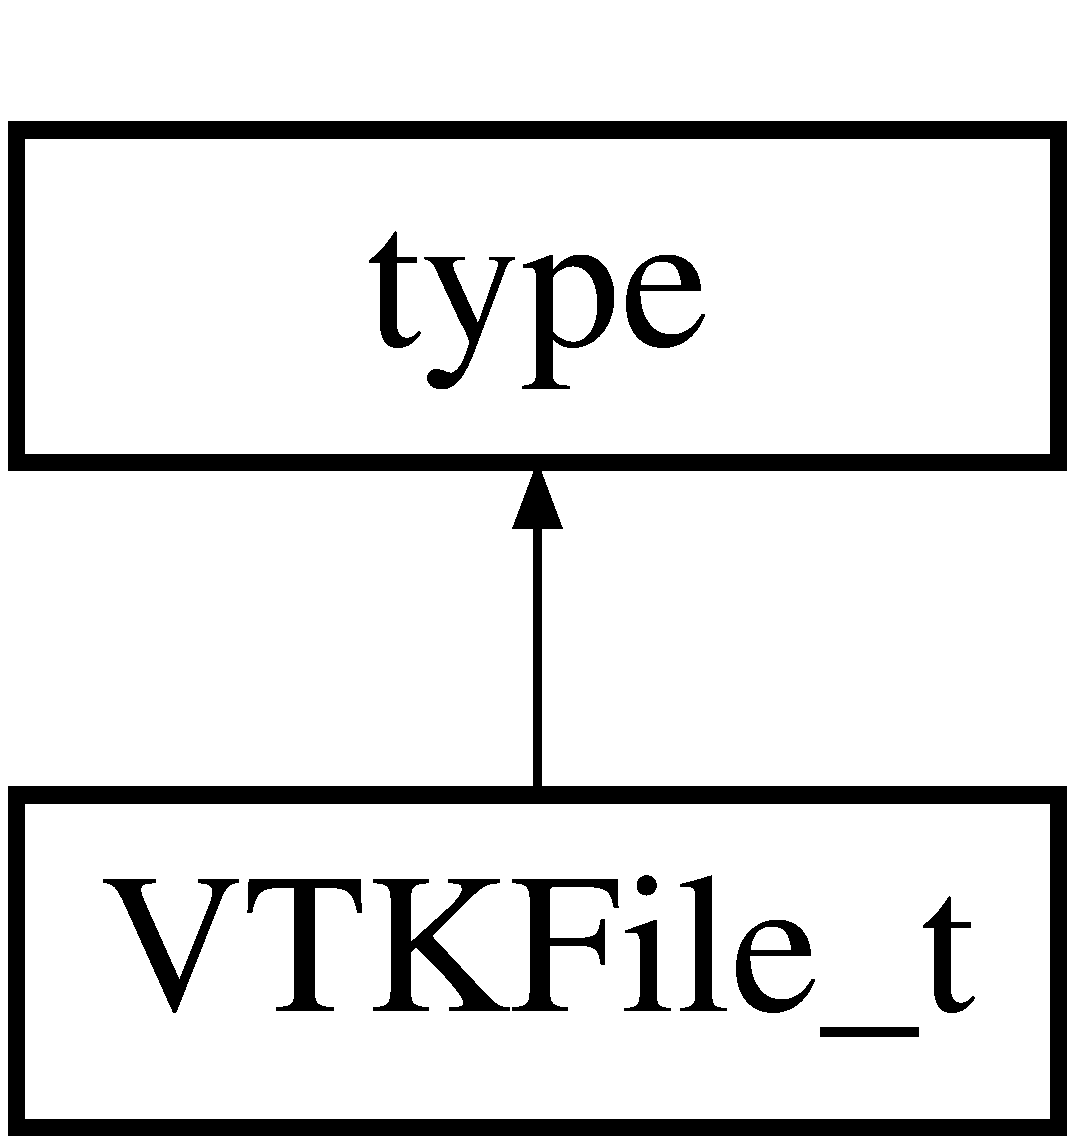
\includegraphics[height=2.000000cm]{classVTKFile__t}
\end{center}
\end{figure}
\subsection*{Public Member Functions}
\begin{DoxyCompactItemize}
\item 
virtual \hyperlink{classVTKFile__t_ac5cf95c81660088dbb3c9ab6cd78dede}{$\sim$\+V\+T\+K\+File\+\_\+t} ()
\begin{DoxyCompactList}\small\item\em Destructor. \end{DoxyCompactList}\end{DoxyCompactItemize}
\subsection*{Unstructured\+Grid}
\label{_amgrp51267337395fceec37fec7e87b9a53e5}%
Accessor and modifier functions for the Unstructured\+Grid optional element. \begin{DoxyCompactItemize}
\item 
typedef \+::\hyperlink{classUnstructuredGrid__t}{Unstructured\+Grid\+\_\+t} \hyperlink{classVTKFile__t_a34ea02f6804e701657f11a8dc3851951}{Unstructured\+Grid\+\_\+type}
\begin{DoxyCompactList}\small\item\em Element type. \end{DoxyCompactList}\item 
typedef \+::xsd\+::cxx\+::tree\+::optional$<$ \hyperlink{classVTKFile__t_a34ea02f6804e701657f11a8dc3851951}{Unstructured\+Grid\+\_\+type} $>$ \hyperlink{classVTKFile__t_ada5bb5a706e03ef1ab2ed1513ea83833}{Unstructured\+Grid\+\_\+optional}
\begin{DoxyCompactList}\small\item\em Element optional container type. \end{DoxyCompactList}\item 
typedef \+::xsd\+::cxx\+::tree\+::traits$<$ \hyperlink{classVTKFile__t_a34ea02f6804e701657f11a8dc3851951}{Unstructured\+Grid\+\_\+type}, char $>$ \hyperlink{classVTKFile__t_a02772a5f713678f02e94188d6a552528}{Unstructured\+Grid\+\_\+traits}
\begin{DoxyCompactList}\small\item\em Element traits type. \end{DoxyCompactList}\item 
const \hyperlink{classVTKFile__t_ada5bb5a706e03ef1ab2ed1513ea83833}{Unstructured\+Grid\+\_\+optional} \& \hyperlink{classVTKFile__t_a118852d8ec1f8039d1fd5c914282351a}{Unstructured\+Grid} () const 
\begin{DoxyCompactList}\small\item\em Return a read-\/only (constant) reference to the element container. \end{DoxyCompactList}\item 
\hyperlink{classVTKFile__t_ada5bb5a706e03ef1ab2ed1513ea83833}{Unstructured\+Grid\+\_\+optional} \& \hyperlink{classVTKFile__t_aa4746d4a723076d4643b8ef16a9c3890}{Unstructured\+Grid} ()
\begin{DoxyCompactList}\small\item\em Return a read-\/write reference to the element container. \end{DoxyCompactList}\item 
void \hyperlink{classVTKFile__t_a2c2b1b2ff487c7e61bcd2875db8747be}{Unstructured\+Grid} (const \hyperlink{classVTKFile__t_a34ea02f6804e701657f11a8dc3851951}{Unstructured\+Grid\+\_\+type} \&x)
\begin{DoxyCompactList}\small\item\em Set the element value. \end{DoxyCompactList}\item 
void \hyperlink{classVTKFile__t_ae33d9781bddb747f9255570b1af2dfeb}{Unstructured\+Grid} (const \hyperlink{classVTKFile__t_ada5bb5a706e03ef1ab2ed1513ea83833}{Unstructured\+Grid\+\_\+optional} \&x)
\begin{DoxyCompactList}\small\item\em Set the element value. \end{DoxyCompactList}\item 
void \hyperlink{classVTKFile__t_af19a966f55acb5f03299af922bd9dd75}{Unstructured\+Grid} (\+::std\+::auto\+\_\+ptr$<$ \hyperlink{classVTKFile__t_a34ea02f6804e701657f11a8dc3851951}{Unstructured\+Grid\+\_\+type} $>$ p)
\begin{DoxyCompactList}\small\item\em Set the element value without copying. \end{DoxyCompactList}\end{DoxyCompactItemize}
\subsection*{Poly\+Data}
\label{_amgrpf4abb74983d657d0185d4dd07cff9b2c}%
Accessor and modifier functions for the Poly\+Data optional element. \begin{DoxyCompactItemize}
\item 
typedef \+::\hyperlink{classPolyData__t}{Poly\+Data\+\_\+t} \hyperlink{classVTKFile__t_a4588b4f0e28ba09aa219bda7e1fc6c97}{Poly\+Data\+\_\+type}
\begin{DoxyCompactList}\small\item\em Element type. \end{DoxyCompactList}\item 
typedef \+::xsd\+::cxx\+::tree\+::optional$<$ \hyperlink{classVTKFile__t_a4588b4f0e28ba09aa219bda7e1fc6c97}{Poly\+Data\+\_\+type} $>$ \hyperlink{classVTKFile__t_aacb796775ae228cd61726a23b809f3e4}{Poly\+Data\+\_\+optional}
\begin{DoxyCompactList}\small\item\em Element optional container type. \end{DoxyCompactList}\item 
typedef \+::xsd\+::cxx\+::tree\+::traits$<$ \hyperlink{classVTKFile__t_a4588b4f0e28ba09aa219bda7e1fc6c97}{Poly\+Data\+\_\+type}, char $>$ \hyperlink{classVTKFile__t_aa5ad98f5709c1e9beec3804a7f42b5f6}{Poly\+Data\+\_\+traits}
\begin{DoxyCompactList}\small\item\em Element traits type. \end{DoxyCompactList}\item 
const \hyperlink{classVTKFile__t_aacb796775ae228cd61726a23b809f3e4}{Poly\+Data\+\_\+optional} \& \hyperlink{classVTKFile__t_a7d728d7f31157fc80117c2f80978344c}{Poly\+Data} () const 
\begin{DoxyCompactList}\small\item\em Return a read-\/only (constant) reference to the element container. \end{DoxyCompactList}\item 
\hyperlink{classVTKFile__t_aacb796775ae228cd61726a23b809f3e4}{Poly\+Data\+\_\+optional} \& \hyperlink{classVTKFile__t_a0f87118c1898bc43619fa0bade52e921}{Poly\+Data} ()
\begin{DoxyCompactList}\small\item\em Return a read-\/write reference to the element container. \end{DoxyCompactList}\item 
void \hyperlink{classVTKFile__t_ab0a3f2aa2894d0384a89a6e5490c9372}{Poly\+Data} (const \hyperlink{classVTKFile__t_a4588b4f0e28ba09aa219bda7e1fc6c97}{Poly\+Data\+\_\+type} \&x)
\begin{DoxyCompactList}\small\item\em Set the element value. \end{DoxyCompactList}\item 
void \hyperlink{classVTKFile__t_a1c2a800d41431c04965c863220a3b1b5}{Poly\+Data} (const \hyperlink{classVTKFile__t_aacb796775ae228cd61726a23b809f3e4}{Poly\+Data\+\_\+optional} \&x)
\begin{DoxyCompactList}\small\item\em Set the element value. \end{DoxyCompactList}\item 
void \hyperlink{classVTKFile__t_a8ae292e04bf2c955d8f50cdeb60f9369}{Poly\+Data} (\+::std\+::auto\+\_\+ptr$<$ \hyperlink{classVTKFile__t_a4588b4f0e28ba09aa219bda7e1fc6c97}{Poly\+Data\+\_\+type} $>$ p)
\begin{DoxyCompactList}\small\item\em Set the element value without copying. \end{DoxyCompactList}\end{DoxyCompactItemize}
\subsection*{type}
\label{_amgrp599dcce2998a6b40b1e38e8c6006cb0a}%
Accessor and modifier functions for the type required attribute. \begin{DoxyCompactItemize}
\item 
typedef \+::\hyperlink{namespacexml__schema_aefbaf353f9a0043af46d23d9040ef268}{xml\+\_\+schema\+::string} \hyperlink{classVTKFile__t_ac1f3484e4fde414849ede43a00955f76}{type\+\_\+type}
\begin{DoxyCompactList}\small\item\em Attribute type. \end{DoxyCompactList}\item 
typedef \+::xsd\+::cxx\+::tree\+::traits$<$ \hyperlink{classVTKFile__t_ac1f3484e4fde414849ede43a00955f76}{type\+\_\+type}, char $>$ \hyperlink{classVTKFile__t_aee4ac167e843e9def1be4f43ad930391}{type\+\_\+traits}
\begin{DoxyCompactList}\small\item\em Attribute traits type. \end{DoxyCompactList}\item 
const \hyperlink{classVTKFile__t_ac1f3484e4fde414849ede43a00955f76}{type\+\_\+type} \& \hyperlink{classVTKFile__t_a5c23301c79cc6a376fe2abce533b2cf7}{type} () const 
\begin{DoxyCompactList}\small\item\em Return a read-\/only (constant) reference to the attribute. \end{DoxyCompactList}\item 
\hyperlink{classVTKFile__t_ac1f3484e4fde414849ede43a00955f76}{type\+\_\+type} \& \hyperlink{classVTKFile__t_abcc8ab822fa4f9e5e5294f5d8cff05c2}{type} ()
\begin{DoxyCompactList}\small\item\em Return a read-\/write reference to the attribute. \end{DoxyCompactList}\item 
void \hyperlink{classVTKFile__t_a6423eb2dc7fa367417df87de4921301e}{type} (const \hyperlink{classVTKFile__t_ac1f3484e4fde414849ede43a00955f76}{type\+\_\+type} \&x)
\begin{DoxyCompactList}\small\item\em Set the attribute value. \end{DoxyCompactList}\item 
void \hyperlink{classVTKFile__t_a380c8628fd1095c88a80a1804837c213}{type} (\+::std\+::auto\+\_\+ptr$<$ \hyperlink{classVTKFile__t_ac1f3484e4fde414849ede43a00955f76}{type\+\_\+type} $>$ p)
\begin{DoxyCompactList}\small\item\em Set the attribute value without copying. \end{DoxyCompactList}\end{DoxyCompactItemize}
\subsection*{version}
\label{_amgrp2af72f100c356273d46284f6fd1dfc08}%
Accessor and modifier functions for the version required attribute. \begin{DoxyCompactItemize}
\item 
typedef \+::\hyperlink{namespacexml__schema_aefbaf353f9a0043af46d23d9040ef268}{xml\+\_\+schema\+::string} \hyperlink{classVTKFile__t_a7db6f6d11f363380d6361446f5dede7b}{version\+\_\+type}
\begin{DoxyCompactList}\small\item\em Attribute type. \end{DoxyCompactList}\item 
typedef \+::xsd\+::cxx\+::tree\+::traits$<$ \hyperlink{classVTKFile__t_a7db6f6d11f363380d6361446f5dede7b}{version\+\_\+type}, char $>$ \hyperlink{classVTKFile__t_a5a343e08417564e5db3f48859b1a0c5f}{version\+\_\+traits}
\begin{DoxyCompactList}\small\item\em Attribute traits type. \end{DoxyCompactList}\item 
const \hyperlink{classVTKFile__t_a7db6f6d11f363380d6361446f5dede7b}{version\+\_\+type} \& \hyperlink{classVTKFile__t_af0f1ed9d44019ad1fab6495b6ae71a47}{version} () const 
\begin{DoxyCompactList}\small\item\em Return a read-\/only (constant) reference to the attribute. \end{DoxyCompactList}\item 
static const \hyperlink{classVTKFile__t_a7db6f6d11f363380d6361446f5dede7b}{version\+\_\+type} \& \hyperlink{classVTKFile__t_a0eb5afa9ec6125c0519a891578f31521}{version\+\_\+default\+\_\+value} ()
\begin{DoxyCompactList}\small\item\em Return the default value for the attribute. \end{DoxyCompactList}\end{DoxyCompactItemize}
\subsection*{byte\+\_\+order}
\label{_amgrp4d85380f9aa2c7bfea4b497dbb3373af}%
Accessor and modifier functions for the byte\+\_\+order required attribute. \begin{DoxyCompactItemize}
\item 
typedef \+::\hyperlink{namespacexml__schema_aefbaf353f9a0043af46d23d9040ef268}{xml\+\_\+schema\+::string} \hyperlink{classVTKFile__t_ab08dd45c560dd0635d0e5c0a5e42d2e8}{byte\+\_\+order\+\_\+type}
\begin{DoxyCompactList}\small\item\em Attribute type. \end{DoxyCompactList}\item 
typedef \+::xsd\+::cxx\+::tree\+::traits$<$ \hyperlink{classVTKFile__t_ab08dd45c560dd0635d0e5c0a5e42d2e8}{byte\+\_\+order\+\_\+type}, char $>$ \hyperlink{classVTKFile__t_ae0b8c254bc373d9218ea9eab406b7b98}{byte\+\_\+order\+\_\+traits}
\begin{DoxyCompactList}\small\item\em Attribute traits type. \end{DoxyCompactList}\item 
const \hyperlink{classVTKFile__t_ab08dd45c560dd0635d0e5c0a5e42d2e8}{byte\+\_\+order\+\_\+type} \& \hyperlink{classVTKFile__t_ad87b4f45ca18139b1ffae8ce08dc2e27}{byte\+\_\+order} () const 
\begin{DoxyCompactList}\small\item\em Return a read-\/only (constant) reference to the attribute. \end{DoxyCompactList}\item 
static const \hyperlink{classVTKFile__t_ab08dd45c560dd0635d0e5c0a5e42d2e8}{byte\+\_\+order\+\_\+type} \& \hyperlink{classVTKFile__t_a4538fe428d79eff40025d874e200bec1}{byte\+\_\+order\+\_\+default\+\_\+value} ()
\begin{DoxyCompactList}\small\item\em Return the default value for the attribute. \end{DoxyCompactList}\end{DoxyCompactItemize}
\subsection*{Constructors}
\begin{DoxyCompactItemize}
\item 
\hyperlink{classVTKFile__t_a76547340cb91ad0019d45889ca69fda0}{V\+T\+K\+File\+\_\+t} (const \hyperlink{classVTKFile__t_ac1f3484e4fde414849ede43a00955f76}{type\+\_\+type} \&)
\begin{DoxyCompactList}\small\item\em Create an instance from the ultimate base and initializers for required elements and attributes. \end{DoxyCompactList}\item 
\hyperlink{classVTKFile__t_a5d1c8c263c9865fe6f4b6ae1446efcaf}{V\+T\+K\+File\+\_\+t} (const \+::xercesc\+::\+D\+O\+M\+Element \&e,\+::\hyperlink{namespacexml__schema_a8d981c127a1f5106d04ad5853e707361}{xml\+\_\+schema\+::flags} f=0,\+::\hyperlink{namespacexml__schema_a395f5179c5fc4643909d66e9ff28d8ca}{xml\+\_\+schema\+::container} $\ast$c=0)
\begin{DoxyCompactList}\small\item\em Create an instance from a D\+O\+M element. \end{DoxyCompactList}\item 
\hyperlink{classVTKFile__t_af239970202f0aee8392cb0af61863f62}{V\+T\+K\+File\+\_\+t} (const \hyperlink{classVTKFile__t}{V\+T\+K\+File\+\_\+t} \&x,\+::\hyperlink{namespacexml__schema_a8d981c127a1f5106d04ad5853e707361}{xml\+\_\+schema\+::flags} f=0,\+::\hyperlink{namespacexml__schema_a395f5179c5fc4643909d66e9ff28d8ca}{xml\+\_\+schema\+::container} $\ast$c=0)
\begin{DoxyCompactList}\small\item\em Copy constructor. \end{DoxyCompactList}\item 
virtual \hyperlink{classVTKFile__t}{V\+T\+K\+File\+\_\+t} $\ast$ \hyperlink{classVTKFile__t_ad39ce94f7390685f9717fd521bac36e3}{\+\_\+clone} (\+::\hyperlink{namespacexml__schema_a8d981c127a1f5106d04ad5853e707361}{xml\+\_\+schema\+::flags} f=0,\+::\hyperlink{namespacexml__schema_a395f5179c5fc4643909d66e9ff28d8ca}{xml\+\_\+schema\+::container} $\ast$c=0) const 
\begin{DoxyCompactList}\small\item\em Copy the instance polymorphically. \end{DoxyCompactList}\end{DoxyCompactItemize}


\subsection{Detailed Description}
Class corresponding to the V\+T\+K\+File\+\_\+t schema type. 

The hello\+\_\+t type consists of a greeting phrase and a collection of names to which this greeting applies. 

\subsection{Member Typedef Documentation}
\hypertarget{classVTKFile__t_ae0b8c254bc373d9218ea9eab406b7b98}{}\index{V\+T\+K\+File\+\_\+t@{V\+T\+K\+File\+\_\+t}!byte\+\_\+order\+\_\+traits@{byte\+\_\+order\+\_\+traits}}
\index{byte\+\_\+order\+\_\+traits@{byte\+\_\+order\+\_\+traits}!V\+T\+K\+File\+\_\+t@{V\+T\+K\+File\+\_\+t}}
\subsubsection[{byte\+\_\+order\+\_\+traits}]{\setlength{\rightskip}{0pt plus 5cm}typedef \+::xsd\+::cxx\+::tree\+::traits$<$ {\bf byte\+\_\+order\+\_\+type}, char $>$ {\bf V\+T\+K\+File\+\_\+t\+::byte\+\_\+order\+\_\+traits}}\label{classVTKFile__t_ae0b8c254bc373d9218ea9eab406b7b98}


Attribute traits type. 

\hypertarget{classVTKFile__t_ab08dd45c560dd0635d0e5c0a5e42d2e8}{}\index{V\+T\+K\+File\+\_\+t@{V\+T\+K\+File\+\_\+t}!byte\+\_\+order\+\_\+type@{byte\+\_\+order\+\_\+type}}
\index{byte\+\_\+order\+\_\+type@{byte\+\_\+order\+\_\+type}!V\+T\+K\+File\+\_\+t@{V\+T\+K\+File\+\_\+t}}
\subsubsection[{byte\+\_\+order\+\_\+type}]{\setlength{\rightskip}{0pt plus 5cm}typedef \+::{\bf xml\+\_\+schema\+::string} {\bf V\+T\+K\+File\+\_\+t\+::byte\+\_\+order\+\_\+type}}\label{classVTKFile__t_ab08dd45c560dd0635d0e5c0a5e42d2e8}


Attribute type. 

\hypertarget{classVTKFile__t_aacb796775ae228cd61726a23b809f3e4}{}\index{V\+T\+K\+File\+\_\+t@{V\+T\+K\+File\+\_\+t}!Poly\+Data\+\_\+optional@{Poly\+Data\+\_\+optional}}
\index{Poly\+Data\+\_\+optional@{Poly\+Data\+\_\+optional}!V\+T\+K\+File\+\_\+t@{V\+T\+K\+File\+\_\+t}}
\subsubsection[{Poly\+Data\+\_\+optional}]{\setlength{\rightskip}{0pt plus 5cm}typedef \+::xsd\+::cxx\+::tree\+::optional$<$ {\bf Poly\+Data\+\_\+type} $>$ {\bf V\+T\+K\+File\+\_\+t\+::\+Poly\+Data\+\_\+optional}}\label{classVTKFile__t_aacb796775ae228cd61726a23b809f3e4}


Element optional container type. 

\hypertarget{classVTKFile__t_aa5ad98f5709c1e9beec3804a7f42b5f6}{}\index{V\+T\+K\+File\+\_\+t@{V\+T\+K\+File\+\_\+t}!Poly\+Data\+\_\+traits@{Poly\+Data\+\_\+traits}}
\index{Poly\+Data\+\_\+traits@{Poly\+Data\+\_\+traits}!V\+T\+K\+File\+\_\+t@{V\+T\+K\+File\+\_\+t}}
\subsubsection[{Poly\+Data\+\_\+traits}]{\setlength{\rightskip}{0pt plus 5cm}typedef \+::xsd\+::cxx\+::tree\+::traits$<$ {\bf Poly\+Data\+\_\+type}, char $>$ {\bf V\+T\+K\+File\+\_\+t\+::\+Poly\+Data\+\_\+traits}}\label{classVTKFile__t_aa5ad98f5709c1e9beec3804a7f42b5f6}


Element traits type. 

\hypertarget{classVTKFile__t_a4588b4f0e28ba09aa219bda7e1fc6c97}{}\index{V\+T\+K\+File\+\_\+t@{V\+T\+K\+File\+\_\+t}!Poly\+Data\+\_\+type@{Poly\+Data\+\_\+type}}
\index{Poly\+Data\+\_\+type@{Poly\+Data\+\_\+type}!V\+T\+K\+File\+\_\+t@{V\+T\+K\+File\+\_\+t}}
\subsubsection[{Poly\+Data\+\_\+type}]{\setlength{\rightskip}{0pt plus 5cm}typedef \+::{\bf Poly\+Data\+\_\+t} {\bf V\+T\+K\+File\+\_\+t\+::\+Poly\+Data\+\_\+type}}\label{classVTKFile__t_a4588b4f0e28ba09aa219bda7e1fc6c97}


Element type. 

\hypertarget{classVTKFile__t_aee4ac167e843e9def1be4f43ad930391}{}\index{V\+T\+K\+File\+\_\+t@{V\+T\+K\+File\+\_\+t}!type\+\_\+traits@{type\+\_\+traits}}
\index{type\+\_\+traits@{type\+\_\+traits}!V\+T\+K\+File\+\_\+t@{V\+T\+K\+File\+\_\+t}}
\subsubsection[{type\+\_\+traits}]{\setlength{\rightskip}{0pt plus 5cm}typedef \+::xsd\+::cxx\+::tree\+::traits$<$ {\bf type\+\_\+type}, char $>$ {\bf V\+T\+K\+File\+\_\+t\+::type\+\_\+traits}}\label{classVTKFile__t_aee4ac167e843e9def1be4f43ad930391}


Attribute traits type. 

\hypertarget{classVTKFile__t_ac1f3484e4fde414849ede43a00955f76}{}\index{V\+T\+K\+File\+\_\+t@{V\+T\+K\+File\+\_\+t}!type\+\_\+type@{type\+\_\+type}}
\index{type\+\_\+type@{type\+\_\+type}!V\+T\+K\+File\+\_\+t@{V\+T\+K\+File\+\_\+t}}
\subsubsection[{type\+\_\+type}]{\setlength{\rightskip}{0pt plus 5cm}typedef \+::{\bf xml\+\_\+schema\+::string} {\bf V\+T\+K\+File\+\_\+t\+::type\+\_\+type}}\label{classVTKFile__t_ac1f3484e4fde414849ede43a00955f76}


Attribute type. 

\hypertarget{classVTKFile__t_ada5bb5a706e03ef1ab2ed1513ea83833}{}\index{V\+T\+K\+File\+\_\+t@{V\+T\+K\+File\+\_\+t}!Unstructured\+Grid\+\_\+optional@{Unstructured\+Grid\+\_\+optional}}
\index{Unstructured\+Grid\+\_\+optional@{Unstructured\+Grid\+\_\+optional}!V\+T\+K\+File\+\_\+t@{V\+T\+K\+File\+\_\+t}}
\subsubsection[{Unstructured\+Grid\+\_\+optional}]{\setlength{\rightskip}{0pt plus 5cm}typedef \+::xsd\+::cxx\+::tree\+::optional$<$ {\bf Unstructured\+Grid\+\_\+type} $>$ {\bf V\+T\+K\+File\+\_\+t\+::\+Unstructured\+Grid\+\_\+optional}}\label{classVTKFile__t_ada5bb5a706e03ef1ab2ed1513ea83833}


Element optional container type. 

\hypertarget{classVTKFile__t_a02772a5f713678f02e94188d6a552528}{}\index{V\+T\+K\+File\+\_\+t@{V\+T\+K\+File\+\_\+t}!Unstructured\+Grid\+\_\+traits@{Unstructured\+Grid\+\_\+traits}}
\index{Unstructured\+Grid\+\_\+traits@{Unstructured\+Grid\+\_\+traits}!V\+T\+K\+File\+\_\+t@{V\+T\+K\+File\+\_\+t}}
\subsubsection[{Unstructured\+Grid\+\_\+traits}]{\setlength{\rightskip}{0pt plus 5cm}typedef \+::xsd\+::cxx\+::tree\+::traits$<$ {\bf Unstructured\+Grid\+\_\+type}, char $>$ {\bf V\+T\+K\+File\+\_\+t\+::\+Unstructured\+Grid\+\_\+traits}}\label{classVTKFile__t_a02772a5f713678f02e94188d6a552528}


Element traits type. 

\hypertarget{classVTKFile__t_a34ea02f6804e701657f11a8dc3851951}{}\index{V\+T\+K\+File\+\_\+t@{V\+T\+K\+File\+\_\+t}!Unstructured\+Grid\+\_\+type@{Unstructured\+Grid\+\_\+type}}
\index{Unstructured\+Grid\+\_\+type@{Unstructured\+Grid\+\_\+type}!V\+T\+K\+File\+\_\+t@{V\+T\+K\+File\+\_\+t}}
\subsubsection[{Unstructured\+Grid\+\_\+type}]{\setlength{\rightskip}{0pt plus 5cm}typedef \+::{\bf Unstructured\+Grid\+\_\+t} {\bf V\+T\+K\+File\+\_\+t\+::\+Unstructured\+Grid\+\_\+type}}\label{classVTKFile__t_a34ea02f6804e701657f11a8dc3851951}


Element type. 

\hypertarget{classVTKFile__t_a5a343e08417564e5db3f48859b1a0c5f}{}\index{V\+T\+K\+File\+\_\+t@{V\+T\+K\+File\+\_\+t}!version\+\_\+traits@{version\+\_\+traits}}
\index{version\+\_\+traits@{version\+\_\+traits}!V\+T\+K\+File\+\_\+t@{V\+T\+K\+File\+\_\+t}}
\subsubsection[{version\+\_\+traits}]{\setlength{\rightskip}{0pt plus 5cm}typedef \+::xsd\+::cxx\+::tree\+::traits$<$ {\bf version\+\_\+type}, char $>$ {\bf V\+T\+K\+File\+\_\+t\+::version\+\_\+traits}}\label{classVTKFile__t_a5a343e08417564e5db3f48859b1a0c5f}


Attribute traits type. 

\hypertarget{classVTKFile__t_a7db6f6d11f363380d6361446f5dede7b}{}\index{V\+T\+K\+File\+\_\+t@{V\+T\+K\+File\+\_\+t}!version\+\_\+type@{version\+\_\+type}}
\index{version\+\_\+type@{version\+\_\+type}!V\+T\+K\+File\+\_\+t@{V\+T\+K\+File\+\_\+t}}
\subsubsection[{version\+\_\+type}]{\setlength{\rightskip}{0pt plus 5cm}typedef \+::{\bf xml\+\_\+schema\+::string} {\bf V\+T\+K\+File\+\_\+t\+::version\+\_\+type}}\label{classVTKFile__t_a7db6f6d11f363380d6361446f5dede7b}


Attribute type. 



\subsection{Constructor \& Destructor Documentation}
\hypertarget{classVTKFile__t_a76547340cb91ad0019d45889ca69fda0}{}\index{V\+T\+K\+File\+\_\+t@{V\+T\+K\+File\+\_\+t}!V\+T\+K\+File\+\_\+t@{V\+T\+K\+File\+\_\+t}}
\index{V\+T\+K\+File\+\_\+t@{V\+T\+K\+File\+\_\+t}!V\+T\+K\+File\+\_\+t@{V\+T\+K\+File\+\_\+t}}
\subsubsection[{V\+T\+K\+File\+\_\+t}]{\setlength{\rightskip}{0pt plus 5cm}V\+T\+K\+File\+\_\+t\+::\+V\+T\+K\+File\+\_\+t (
\begin{DoxyParamCaption}
\item[{const {\bf type\+\_\+type} \&}]{type}
\end{DoxyParamCaption}
)}\label{classVTKFile__t_a76547340cb91ad0019d45889ca69fda0}


Create an instance from the ultimate base and initializers for required elements and attributes. 

\hypertarget{classVTKFile__t_a5d1c8c263c9865fe6f4b6ae1446efcaf}{}\index{V\+T\+K\+File\+\_\+t@{V\+T\+K\+File\+\_\+t}!V\+T\+K\+File\+\_\+t@{V\+T\+K\+File\+\_\+t}}
\index{V\+T\+K\+File\+\_\+t@{V\+T\+K\+File\+\_\+t}!V\+T\+K\+File\+\_\+t@{V\+T\+K\+File\+\_\+t}}
\subsubsection[{V\+T\+K\+File\+\_\+t}]{\setlength{\rightskip}{0pt plus 5cm}V\+T\+K\+File\+\_\+t\+::\+V\+T\+K\+File\+\_\+t (
\begin{DoxyParamCaption}
\item[{const \+::xercesc\+::\+D\+O\+M\+Element \&}]{e, }
\item[{\+::{\bf xml\+\_\+schema\+::flags}}]{f = {\ttfamily 0}, }
\item[{\+::{\bf xml\+\_\+schema\+::container} $\ast$}]{c = {\ttfamily 0}}
\end{DoxyParamCaption}
)}\label{classVTKFile__t_a5d1c8c263c9865fe6f4b6ae1446efcaf}


Create an instance from a D\+O\+M element. 


\begin{DoxyParams}{Parameters}
{\em e} & A D\+O\+M element to extract the data from. \\
\hline
{\em f} & Flags to create the new instance with. \\
\hline
{\em c} & A pointer to the object that will contain the new instance. \\
\hline
\end{DoxyParams}
\hypertarget{classVTKFile__t_af239970202f0aee8392cb0af61863f62}{}\index{V\+T\+K\+File\+\_\+t@{V\+T\+K\+File\+\_\+t}!V\+T\+K\+File\+\_\+t@{V\+T\+K\+File\+\_\+t}}
\index{V\+T\+K\+File\+\_\+t@{V\+T\+K\+File\+\_\+t}!V\+T\+K\+File\+\_\+t@{V\+T\+K\+File\+\_\+t}}
\subsubsection[{V\+T\+K\+File\+\_\+t}]{\setlength{\rightskip}{0pt plus 5cm}V\+T\+K\+File\+\_\+t\+::\+V\+T\+K\+File\+\_\+t (
\begin{DoxyParamCaption}
\item[{const {\bf V\+T\+K\+File\+\_\+t} \&}]{x, }
\item[{\+::{\bf xml\+\_\+schema\+::flags}}]{f = {\ttfamily 0}, }
\item[{\+::{\bf xml\+\_\+schema\+::container} $\ast$}]{c = {\ttfamily 0}}
\end{DoxyParamCaption}
)}\label{classVTKFile__t_af239970202f0aee8392cb0af61863f62}


Copy constructor. 


\begin{DoxyParams}{Parameters}
{\em x} & An instance to make a copy of. \\
\hline
{\em f} & Flags to create the copy with. \\
\hline
{\em c} & A pointer to the object that will contain the copy.\\
\hline
\end{DoxyParams}
For polymorphic object models use the {\ttfamily \+\_\+clone} function instead. \hypertarget{classVTKFile__t_ac5cf95c81660088dbb3c9ab6cd78dede}{}\index{V\+T\+K\+File\+\_\+t@{V\+T\+K\+File\+\_\+t}!````~V\+T\+K\+File\+\_\+t@{$\sim$\+V\+T\+K\+File\+\_\+t}}
\index{````~V\+T\+K\+File\+\_\+t@{$\sim$\+V\+T\+K\+File\+\_\+t}!V\+T\+K\+File\+\_\+t@{V\+T\+K\+File\+\_\+t}}
\subsubsection[{$\sim$\+V\+T\+K\+File\+\_\+t}]{\setlength{\rightskip}{0pt plus 5cm}V\+T\+K\+File\+\_\+t\+::$\sim$\+V\+T\+K\+File\+\_\+t (
\begin{DoxyParamCaption}
{}
\end{DoxyParamCaption}
)\hspace{0.3cm}{\ttfamily [virtual]}}\label{classVTKFile__t_ac5cf95c81660088dbb3c9ab6cd78dede}


Destructor. 



\subsection{Member Function Documentation}
\hypertarget{classVTKFile__t_ad39ce94f7390685f9717fd521bac36e3}{}\index{V\+T\+K\+File\+\_\+t@{V\+T\+K\+File\+\_\+t}!\+\_\+clone@{\+\_\+clone}}
\index{\+\_\+clone@{\+\_\+clone}!V\+T\+K\+File\+\_\+t@{V\+T\+K\+File\+\_\+t}}
\subsubsection[{\+\_\+clone}]{\setlength{\rightskip}{0pt plus 5cm}{\bf V\+T\+K\+File\+\_\+t} $\ast$ V\+T\+K\+File\+\_\+t\+::\+\_\+clone (
\begin{DoxyParamCaption}
\item[{\+::{\bf xml\+\_\+schema\+::flags}}]{f = {\ttfamily 0}, }
\item[{\+::{\bf xml\+\_\+schema\+::container} $\ast$}]{c = {\ttfamily 0}}
\end{DoxyParamCaption}
) const\hspace{0.3cm}{\ttfamily [virtual]}}\label{classVTKFile__t_ad39ce94f7390685f9717fd521bac36e3}


Copy the instance polymorphically. 


\begin{DoxyParams}{Parameters}
{\em f} & Flags to create the copy with. \\
\hline
{\em c} & A pointer to the object that will contain the copy. \\
\hline
\end{DoxyParams}
\begin{DoxyReturn}{Returns}
A pointer to the dynamically allocated copy.
\end{DoxyReturn}
This function ensures that the dynamic type of the instance is used for copying and should be used for polymorphic object models instead of the copy constructor. \hypertarget{classVTKFile__t_ad87b4f45ca18139b1ffae8ce08dc2e27}{}\index{V\+T\+K\+File\+\_\+t@{V\+T\+K\+File\+\_\+t}!byte\+\_\+order@{byte\+\_\+order}}
\index{byte\+\_\+order@{byte\+\_\+order}!V\+T\+K\+File\+\_\+t@{V\+T\+K\+File\+\_\+t}}
\subsubsection[{byte\+\_\+order}]{\setlength{\rightskip}{0pt plus 5cm}const {\bf V\+T\+K\+File\+\_\+t\+::byte\+\_\+order\+\_\+type} \& V\+T\+K\+File\+\_\+t\+::byte\+\_\+order (
\begin{DoxyParamCaption}
{}
\end{DoxyParamCaption}
) const}\label{classVTKFile__t_ad87b4f45ca18139b1ffae8ce08dc2e27}


Return a read-\/only (constant) reference to the attribute. 

\begin{DoxyReturn}{Returns}
A constant reference to the attribute. 
\end{DoxyReturn}
\hypertarget{classVTKFile__t_a4538fe428d79eff40025d874e200bec1}{}\index{V\+T\+K\+File\+\_\+t@{V\+T\+K\+File\+\_\+t}!byte\+\_\+order\+\_\+default\+\_\+value@{byte\+\_\+order\+\_\+default\+\_\+value}}
\index{byte\+\_\+order\+\_\+default\+\_\+value@{byte\+\_\+order\+\_\+default\+\_\+value}!V\+T\+K\+File\+\_\+t@{V\+T\+K\+File\+\_\+t}}
\subsubsection[{byte\+\_\+order\+\_\+default\+\_\+value}]{\setlength{\rightskip}{0pt plus 5cm}const {\bf V\+T\+K\+File\+\_\+t\+::byte\+\_\+order\+\_\+type} \& V\+T\+K\+File\+\_\+t\+::byte\+\_\+order\+\_\+default\+\_\+value (
\begin{DoxyParamCaption}
{}
\end{DoxyParamCaption}
)\hspace{0.3cm}{\ttfamily [static]}}\label{classVTKFile__t_a4538fe428d79eff40025d874e200bec1}


Return the default value for the attribute. 

\begin{DoxyReturn}{Returns}
A read-\/only (constant) reference to the attribute\textquotesingle{}s default value. 
\end{DoxyReturn}
\hypertarget{classVTKFile__t_a7d728d7f31157fc80117c2f80978344c}{}\index{V\+T\+K\+File\+\_\+t@{V\+T\+K\+File\+\_\+t}!Poly\+Data@{Poly\+Data}}
\index{Poly\+Data@{Poly\+Data}!V\+T\+K\+File\+\_\+t@{V\+T\+K\+File\+\_\+t}}
\subsubsection[{Poly\+Data}]{\setlength{\rightskip}{0pt plus 5cm}const {\bf V\+T\+K\+File\+\_\+t\+::\+Poly\+Data\+\_\+optional} \& V\+T\+K\+File\+\_\+t\+::\+Poly\+Data (
\begin{DoxyParamCaption}
{}
\end{DoxyParamCaption}
) const}\label{classVTKFile__t_a7d728d7f31157fc80117c2f80978344c}


Return a read-\/only (constant) reference to the element container. 

\begin{DoxyReturn}{Returns}
A constant reference to the optional container. 
\end{DoxyReturn}
\hypertarget{classVTKFile__t_a0f87118c1898bc43619fa0bade52e921}{}\index{V\+T\+K\+File\+\_\+t@{V\+T\+K\+File\+\_\+t}!Poly\+Data@{Poly\+Data}}
\index{Poly\+Data@{Poly\+Data}!V\+T\+K\+File\+\_\+t@{V\+T\+K\+File\+\_\+t}}
\subsubsection[{Poly\+Data}]{\setlength{\rightskip}{0pt plus 5cm}{\bf V\+T\+K\+File\+\_\+t\+::\+Poly\+Data\+\_\+optional} \& V\+T\+K\+File\+\_\+t\+::\+Poly\+Data (
\begin{DoxyParamCaption}
{}
\end{DoxyParamCaption}
)}\label{classVTKFile__t_a0f87118c1898bc43619fa0bade52e921}


Return a read-\/write reference to the element container. 

\begin{DoxyReturn}{Returns}
A reference to the optional container. 
\end{DoxyReturn}
\hypertarget{classVTKFile__t_ab0a3f2aa2894d0384a89a6e5490c9372}{}\index{V\+T\+K\+File\+\_\+t@{V\+T\+K\+File\+\_\+t}!Poly\+Data@{Poly\+Data}}
\index{Poly\+Data@{Poly\+Data}!V\+T\+K\+File\+\_\+t@{V\+T\+K\+File\+\_\+t}}
\subsubsection[{Poly\+Data}]{\setlength{\rightskip}{0pt plus 5cm}void V\+T\+K\+File\+\_\+t\+::\+Poly\+Data (
\begin{DoxyParamCaption}
\item[{const {\bf Poly\+Data\+\_\+type} \&}]{x}
\end{DoxyParamCaption}
)}\label{classVTKFile__t_ab0a3f2aa2894d0384a89a6e5490c9372}


Set the element value. 


\begin{DoxyParams}{Parameters}
{\em x} & A new value to set.\\
\hline
\end{DoxyParams}
This function makes a copy of its argument and sets it as the new value of the element. \hypertarget{classVTKFile__t_a1c2a800d41431c04965c863220a3b1b5}{}\index{V\+T\+K\+File\+\_\+t@{V\+T\+K\+File\+\_\+t}!Poly\+Data@{Poly\+Data}}
\index{Poly\+Data@{Poly\+Data}!V\+T\+K\+File\+\_\+t@{V\+T\+K\+File\+\_\+t}}
\subsubsection[{Poly\+Data}]{\setlength{\rightskip}{0pt plus 5cm}void V\+T\+K\+File\+\_\+t\+::\+Poly\+Data (
\begin{DoxyParamCaption}
\item[{const {\bf Poly\+Data\+\_\+optional} \&}]{x}
\end{DoxyParamCaption}
)}\label{classVTKFile__t_a1c2a800d41431c04965c863220a3b1b5}


Set the element value. 


\begin{DoxyParams}{Parameters}
{\em x} & An optional container with the new value to set.\\
\hline
\end{DoxyParams}
If the value is present in {\itshape x} then this function makes a copy of this value and sets it as the new value of the element. Otherwise the element container is set the \textquotesingle{}not present\textquotesingle{} state. \hypertarget{classVTKFile__t_a8ae292e04bf2c955d8f50cdeb60f9369}{}\index{V\+T\+K\+File\+\_\+t@{V\+T\+K\+File\+\_\+t}!Poly\+Data@{Poly\+Data}}
\index{Poly\+Data@{Poly\+Data}!V\+T\+K\+File\+\_\+t@{V\+T\+K\+File\+\_\+t}}
\subsubsection[{Poly\+Data}]{\setlength{\rightskip}{0pt plus 5cm}void V\+T\+K\+File\+\_\+t\+::\+Poly\+Data (
\begin{DoxyParamCaption}
\item[{\+::std\+::auto\+\_\+ptr$<$ {\bf Poly\+Data\+\_\+type} $>$}]{p}
\end{DoxyParamCaption}
)}\label{classVTKFile__t_a8ae292e04bf2c955d8f50cdeb60f9369}


Set the element value without copying. 


\begin{DoxyParams}{Parameters}
{\em p} & A new value to use.\\
\hline
\end{DoxyParams}
This function will try to use the passed value directly instead of making a copy. \hypertarget{classVTKFile__t_a5c23301c79cc6a376fe2abce533b2cf7}{}\index{V\+T\+K\+File\+\_\+t@{V\+T\+K\+File\+\_\+t}!type@{type}}
\index{type@{type}!V\+T\+K\+File\+\_\+t@{V\+T\+K\+File\+\_\+t}}
\subsubsection[{type}]{\setlength{\rightskip}{0pt plus 5cm}const {\bf V\+T\+K\+File\+\_\+t\+::type\+\_\+type} \& V\+T\+K\+File\+\_\+t\+::type (
\begin{DoxyParamCaption}
{}
\end{DoxyParamCaption}
) const}\label{classVTKFile__t_a5c23301c79cc6a376fe2abce533b2cf7}


Return a read-\/only (constant) reference to the attribute. 

\begin{DoxyReturn}{Returns}
A constant reference to the attribute. 
\end{DoxyReturn}
\hypertarget{classVTKFile__t_abcc8ab822fa4f9e5e5294f5d8cff05c2}{}\index{V\+T\+K\+File\+\_\+t@{V\+T\+K\+File\+\_\+t}!type@{type}}
\index{type@{type}!V\+T\+K\+File\+\_\+t@{V\+T\+K\+File\+\_\+t}}
\subsubsection[{type}]{\setlength{\rightskip}{0pt plus 5cm}{\bf V\+T\+K\+File\+\_\+t\+::type\+\_\+type} \& V\+T\+K\+File\+\_\+t\+::type (
\begin{DoxyParamCaption}
{}
\end{DoxyParamCaption}
)}\label{classVTKFile__t_abcc8ab822fa4f9e5e5294f5d8cff05c2}


Return a read-\/write reference to the attribute. 

\begin{DoxyReturn}{Returns}
A reference to the attribute. 
\end{DoxyReturn}
\hypertarget{classVTKFile__t_a6423eb2dc7fa367417df87de4921301e}{}\index{V\+T\+K\+File\+\_\+t@{V\+T\+K\+File\+\_\+t}!type@{type}}
\index{type@{type}!V\+T\+K\+File\+\_\+t@{V\+T\+K\+File\+\_\+t}}
\subsubsection[{type}]{\setlength{\rightskip}{0pt plus 5cm}void V\+T\+K\+File\+\_\+t\+::type (
\begin{DoxyParamCaption}
\item[{const {\bf type\+\_\+type} \&}]{x}
\end{DoxyParamCaption}
)}\label{classVTKFile__t_a6423eb2dc7fa367417df87de4921301e}


Set the attribute value. 


\begin{DoxyParams}{Parameters}
{\em x} & A new value to set.\\
\hline
\end{DoxyParams}
This function makes a copy of its argument and sets it as the new value of the attribute. \hypertarget{classVTKFile__t_a380c8628fd1095c88a80a1804837c213}{}\index{V\+T\+K\+File\+\_\+t@{V\+T\+K\+File\+\_\+t}!type@{type}}
\index{type@{type}!V\+T\+K\+File\+\_\+t@{V\+T\+K\+File\+\_\+t}}
\subsubsection[{type}]{\setlength{\rightskip}{0pt plus 5cm}void V\+T\+K\+File\+\_\+t\+::type (
\begin{DoxyParamCaption}
\item[{\+::std\+::auto\+\_\+ptr$<$ {\bf type\+\_\+type} $>$}]{p}
\end{DoxyParamCaption}
)}\label{classVTKFile__t_a380c8628fd1095c88a80a1804837c213}


Set the attribute value without copying. 


\begin{DoxyParams}{Parameters}
{\em p} & A new value to use.\\
\hline
\end{DoxyParams}
This function will try to use the passed value directly instead of making a copy. \hypertarget{classVTKFile__t_a118852d8ec1f8039d1fd5c914282351a}{}\index{V\+T\+K\+File\+\_\+t@{V\+T\+K\+File\+\_\+t}!Unstructured\+Grid@{Unstructured\+Grid}}
\index{Unstructured\+Grid@{Unstructured\+Grid}!V\+T\+K\+File\+\_\+t@{V\+T\+K\+File\+\_\+t}}
\subsubsection[{Unstructured\+Grid}]{\setlength{\rightskip}{0pt plus 5cm}const {\bf V\+T\+K\+File\+\_\+t\+::\+Unstructured\+Grid\+\_\+optional} \& V\+T\+K\+File\+\_\+t\+::\+Unstructured\+Grid (
\begin{DoxyParamCaption}
{}
\end{DoxyParamCaption}
) const}\label{classVTKFile__t_a118852d8ec1f8039d1fd5c914282351a}


Return a read-\/only (constant) reference to the element container. 

\begin{DoxyReturn}{Returns}
A constant reference to the optional container. 
\end{DoxyReturn}
\hypertarget{classVTKFile__t_aa4746d4a723076d4643b8ef16a9c3890}{}\index{V\+T\+K\+File\+\_\+t@{V\+T\+K\+File\+\_\+t}!Unstructured\+Grid@{Unstructured\+Grid}}
\index{Unstructured\+Grid@{Unstructured\+Grid}!V\+T\+K\+File\+\_\+t@{V\+T\+K\+File\+\_\+t}}
\subsubsection[{Unstructured\+Grid}]{\setlength{\rightskip}{0pt plus 5cm}{\bf V\+T\+K\+File\+\_\+t\+::\+Unstructured\+Grid\+\_\+optional} \& V\+T\+K\+File\+\_\+t\+::\+Unstructured\+Grid (
\begin{DoxyParamCaption}
{}
\end{DoxyParamCaption}
)}\label{classVTKFile__t_aa4746d4a723076d4643b8ef16a9c3890}


Return a read-\/write reference to the element container. 

\begin{DoxyReturn}{Returns}
A reference to the optional container. 
\end{DoxyReturn}
\hypertarget{classVTKFile__t_a2c2b1b2ff487c7e61bcd2875db8747be}{}\index{V\+T\+K\+File\+\_\+t@{V\+T\+K\+File\+\_\+t}!Unstructured\+Grid@{Unstructured\+Grid}}
\index{Unstructured\+Grid@{Unstructured\+Grid}!V\+T\+K\+File\+\_\+t@{V\+T\+K\+File\+\_\+t}}
\subsubsection[{Unstructured\+Grid}]{\setlength{\rightskip}{0pt plus 5cm}void V\+T\+K\+File\+\_\+t\+::\+Unstructured\+Grid (
\begin{DoxyParamCaption}
\item[{const {\bf Unstructured\+Grid\+\_\+type} \&}]{x}
\end{DoxyParamCaption}
)}\label{classVTKFile__t_a2c2b1b2ff487c7e61bcd2875db8747be}


Set the element value. 


\begin{DoxyParams}{Parameters}
{\em x} & A new value to set.\\
\hline
\end{DoxyParams}
This function makes a copy of its argument and sets it as the new value of the element. \hypertarget{classVTKFile__t_ae33d9781bddb747f9255570b1af2dfeb}{}\index{V\+T\+K\+File\+\_\+t@{V\+T\+K\+File\+\_\+t}!Unstructured\+Grid@{Unstructured\+Grid}}
\index{Unstructured\+Grid@{Unstructured\+Grid}!V\+T\+K\+File\+\_\+t@{V\+T\+K\+File\+\_\+t}}
\subsubsection[{Unstructured\+Grid}]{\setlength{\rightskip}{0pt plus 5cm}void V\+T\+K\+File\+\_\+t\+::\+Unstructured\+Grid (
\begin{DoxyParamCaption}
\item[{const {\bf Unstructured\+Grid\+\_\+optional} \&}]{x}
\end{DoxyParamCaption}
)}\label{classVTKFile__t_ae33d9781bddb747f9255570b1af2dfeb}


Set the element value. 


\begin{DoxyParams}{Parameters}
{\em x} & An optional container with the new value to set.\\
\hline
\end{DoxyParams}
If the value is present in {\itshape x} then this function makes a copy of this value and sets it as the new value of the element. Otherwise the element container is set the \textquotesingle{}not present\textquotesingle{} state. \hypertarget{classVTKFile__t_af19a966f55acb5f03299af922bd9dd75}{}\index{V\+T\+K\+File\+\_\+t@{V\+T\+K\+File\+\_\+t}!Unstructured\+Grid@{Unstructured\+Grid}}
\index{Unstructured\+Grid@{Unstructured\+Grid}!V\+T\+K\+File\+\_\+t@{V\+T\+K\+File\+\_\+t}}
\subsubsection[{Unstructured\+Grid}]{\setlength{\rightskip}{0pt plus 5cm}void V\+T\+K\+File\+\_\+t\+::\+Unstructured\+Grid (
\begin{DoxyParamCaption}
\item[{\+::std\+::auto\+\_\+ptr$<$ {\bf Unstructured\+Grid\+\_\+type} $>$}]{p}
\end{DoxyParamCaption}
)}\label{classVTKFile__t_af19a966f55acb5f03299af922bd9dd75}


Set the element value without copying. 


\begin{DoxyParams}{Parameters}
{\em p} & A new value to use.\\
\hline
\end{DoxyParams}
This function will try to use the passed value directly instead of making a copy. \hypertarget{classVTKFile__t_af0f1ed9d44019ad1fab6495b6ae71a47}{}\index{V\+T\+K\+File\+\_\+t@{V\+T\+K\+File\+\_\+t}!version@{version}}
\index{version@{version}!V\+T\+K\+File\+\_\+t@{V\+T\+K\+File\+\_\+t}}
\subsubsection[{version}]{\setlength{\rightskip}{0pt plus 5cm}const {\bf V\+T\+K\+File\+\_\+t\+::version\+\_\+type} \& V\+T\+K\+File\+\_\+t\+::version (
\begin{DoxyParamCaption}
{}
\end{DoxyParamCaption}
) const}\label{classVTKFile__t_af0f1ed9d44019ad1fab6495b6ae71a47}


Return a read-\/only (constant) reference to the attribute. 

\begin{DoxyReturn}{Returns}
A constant reference to the attribute. 
\end{DoxyReturn}
\hypertarget{classVTKFile__t_a0eb5afa9ec6125c0519a891578f31521}{}\index{V\+T\+K\+File\+\_\+t@{V\+T\+K\+File\+\_\+t}!version\+\_\+default\+\_\+value@{version\+\_\+default\+\_\+value}}
\index{version\+\_\+default\+\_\+value@{version\+\_\+default\+\_\+value}!V\+T\+K\+File\+\_\+t@{V\+T\+K\+File\+\_\+t}}
\subsubsection[{version\+\_\+default\+\_\+value}]{\setlength{\rightskip}{0pt plus 5cm}const {\bf V\+T\+K\+File\+\_\+t\+::version\+\_\+type} \& V\+T\+K\+File\+\_\+t\+::version\+\_\+default\+\_\+value (
\begin{DoxyParamCaption}
{}
\end{DoxyParamCaption}
)\hspace{0.3cm}{\ttfamily [static]}}\label{classVTKFile__t_a0eb5afa9ec6125c0519a891578f31521}


Return the default value for the attribute. 

\begin{DoxyReturn}{Returns}
A read-\/only (constant) reference to the attribute\textquotesingle{}s default value. 
\end{DoxyReturn}


The documentation for this class was generated from the following files\+:\begin{DoxyCompactItemize}
\item 
src/output\+Writer/\hyperlink{vtk-unstructured_8h}{vtk-\/unstructured.\+h}\item 
src/output\+Writer/\hyperlink{vtk-unstructured_8cpp}{vtk-\/unstructured.\+cpp}\end{DoxyCompactItemize}

\hypertarget{classoutputWriter_1_1VTKWriter}{}\section{output\+Writer\+:\+:V\+T\+K\+Writer Class Reference}
\label{classoutputWriter_1_1VTKWriter}\index{output\+Writer\+::\+V\+T\+K\+Writer@{output\+Writer\+::\+V\+T\+K\+Writer}}


{\ttfamily \#include $<$V\+T\+K\+Writer.\+h$>$}

\subsection*{Public Member Functions}
\begin{DoxyCompactItemize}
\item 
\hyperlink{classoutputWriter_1_1VTKWriter_a448311c322544e40c6e0a3c158924583}{V\+T\+K\+Writer} ()
\item 
virtual \hyperlink{classoutputWriter_1_1VTKWriter_a196a54bcfa3f93638ef292c386f91b61}{$\sim$\+V\+T\+K\+Writer} ()
\item 
void \hyperlink{classoutputWriter_1_1VTKWriter_a41cfcefce4d7eb434f1dd45f5aeb3e8f}{initialize\+Output} (int num\+Particles)
\item 
void \hyperlink{classoutputWriter_1_1VTKWriter_a6d3f50ca3ae2390055d3f9cc0ed1eb4d}{plot\+Particle} (\hyperlink{classParticle}{Particle} \&p)
\item 
void \hyperlink{classoutputWriter_1_1VTKWriter_ad0d7afb78a2027d05e9a03acde3799dd}{write\+File} (const std\+::string \&filename, int iteration)
\end{DoxyCompactItemize}
\subsection*{Private Attributes}
\begin{DoxyCompactItemize}
\item 
\hyperlink{classVTKFile__t}{V\+T\+K\+File\+\_\+t} $\ast$ \hyperlink{classoutputWriter_1_1VTKWriter_ab654ea4308b92e5dbdcd9a6833d5ed30}{vtk\+File}
\end{DoxyCompactItemize}


\subsection{Detailed Description}
This class implements the functionality to generate vtk output from particles. 

\subsection{Constructor \& Destructor Documentation}
\hypertarget{classoutputWriter_1_1VTKWriter_a448311c322544e40c6e0a3c158924583}{}\index{output\+Writer\+::\+V\+T\+K\+Writer@{output\+Writer\+::\+V\+T\+K\+Writer}!V\+T\+K\+Writer@{V\+T\+K\+Writer}}
\index{V\+T\+K\+Writer@{V\+T\+K\+Writer}!output\+Writer\+::\+V\+T\+K\+Writer@{output\+Writer\+::\+V\+T\+K\+Writer}}
\subsubsection[{V\+T\+K\+Writer}]{\setlength{\rightskip}{0pt plus 5cm}output\+Writer\+::\+V\+T\+K\+Writer\+::\+V\+T\+K\+Writer (
\begin{DoxyParamCaption}
{}
\end{DoxyParamCaption}
)}\label{classoutputWriter_1_1VTKWriter_a448311c322544e40c6e0a3c158924583}
\hypertarget{classoutputWriter_1_1VTKWriter_a196a54bcfa3f93638ef292c386f91b61}{}\index{output\+Writer\+::\+V\+T\+K\+Writer@{output\+Writer\+::\+V\+T\+K\+Writer}!````~V\+T\+K\+Writer@{$\sim$\+V\+T\+K\+Writer}}
\index{````~V\+T\+K\+Writer@{$\sim$\+V\+T\+K\+Writer}!output\+Writer\+::\+V\+T\+K\+Writer@{output\+Writer\+::\+V\+T\+K\+Writer}}
\subsubsection[{$\sim$\+V\+T\+K\+Writer}]{\setlength{\rightskip}{0pt plus 5cm}output\+Writer\+::\+V\+T\+K\+Writer\+::$\sim$\+V\+T\+K\+Writer (
\begin{DoxyParamCaption}
{}
\end{DoxyParamCaption}
)\hspace{0.3cm}{\ttfamily [virtual]}}\label{classoutputWriter_1_1VTKWriter_a196a54bcfa3f93638ef292c386f91b61}


\subsection{Member Function Documentation}
\hypertarget{classoutputWriter_1_1VTKWriter_a41cfcefce4d7eb434f1dd45f5aeb3e8f}{}\index{output\+Writer\+::\+V\+T\+K\+Writer@{output\+Writer\+::\+V\+T\+K\+Writer}!initialize\+Output@{initialize\+Output}}
\index{initialize\+Output@{initialize\+Output}!output\+Writer\+::\+V\+T\+K\+Writer@{output\+Writer\+::\+V\+T\+K\+Writer}}
\subsubsection[{initialize\+Output}]{\setlength{\rightskip}{0pt plus 5cm}void output\+Writer\+::\+V\+T\+K\+Writer\+::initialize\+Output (
\begin{DoxyParamCaption}
\item[{int}]{num\+Particles}
\end{DoxyParamCaption}
)}\label{classoutputWriter_1_1VTKWriter_a41cfcefce4d7eb434f1dd45f5aeb3e8f}
set up internal data structures and prepare to plot a particle. \hypertarget{classoutputWriter_1_1VTKWriter_a6d3f50ca3ae2390055d3f9cc0ed1eb4d}{}\index{output\+Writer\+::\+V\+T\+K\+Writer@{output\+Writer\+::\+V\+T\+K\+Writer}!plot\+Particle@{plot\+Particle}}
\index{plot\+Particle@{plot\+Particle}!output\+Writer\+::\+V\+T\+K\+Writer@{output\+Writer\+::\+V\+T\+K\+Writer}}
\subsubsection[{plot\+Particle}]{\setlength{\rightskip}{0pt plus 5cm}void output\+Writer\+::\+V\+T\+K\+Writer\+::plot\+Particle (
\begin{DoxyParamCaption}
\item[{{\bf Particle} \&}]{p}
\end{DoxyParamCaption}
)}\label{classoutputWriter_1_1VTKWriter_a6d3f50ca3ae2390055d3f9cc0ed1eb4d}
plot type, mass, position, velocity and force of a particle.

\begin{DoxyNote}{Note}
\+: \hyperlink{classoutputWriter_1_1VTKWriter_a41cfcefce4d7eb434f1dd45f5aeb3e8f}{initialize\+Output()} must have been called before. 
\end{DoxyNote}
\hypertarget{classoutputWriter_1_1VTKWriter_ad0d7afb78a2027d05e9a03acde3799dd}{}\index{output\+Writer\+::\+V\+T\+K\+Writer@{output\+Writer\+::\+V\+T\+K\+Writer}!write\+File@{write\+File}}
\index{write\+File@{write\+File}!output\+Writer\+::\+V\+T\+K\+Writer@{output\+Writer\+::\+V\+T\+K\+Writer}}
\subsubsection[{write\+File}]{\setlength{\rightskip}{0pt plus 5cm}void output\+Writer\+::\+V\+T\+K\+Writer\+::write\+File (
\begin{DoxyParamCaption}
\item[{const std\+::string \&}]{filename, }
\item[{int}]{iteration}
\end{DoxyParamCaption}
)}\label{classoutputWriter_1_1VTKWriter_ad0d7afb78a2027d05e9a03acde3799dd}
writes the final output file.


\begin{DoxyParams}{Parameters}
{\em filename} & the base name of the file to be written. \\
\hline
{\em iteration} & the number of the current iteration, which is used to generate an unique filename \\
\hline
\end{DoxyParams}


\subsection{Member Data Documentation}
\hypertarget{classoutputWriter_1_1VTKWriter_ab654ea4308b92e5dbdcd9a6833d5ed30}{}\index{output\+Writer\+::\+V\+T\+K\+Writer@{output\+Writer\+::\+V\+T\+K\+Writer}!vtk\+File@{vtk\+File}}
\index{vtk\+File@{vtk\+File}!output\+Writer\+::\+V\+T\+K\+Writer@{output\+Writer\+::\+V\+T\+K\+Writer}}
\subsubsection[{vtk\+File}]{\setlength{\rightskip}{0pt plus 5cm}{\bf V\+T\+K\+File\+\_\+t}$\ast$ output\+Writer\+::\+V\+T\+K\+Writer\+::vtk\+File\hspace{0.3cm}{\ttfamily [private]}}\label{classoutputWriter_1_1VTKWriter_ab654ea4308b92e5dbdcd9a6833d5ed30}


The documentation for this class was generated from the following files\+:\begin{DoxyCompactItemize}
\item 
src/output\+Writer/\hyperlink{VTKWriter_8h}{V\+T\+K\+Writer.\+h}\item 
src/output\+Writer/\hyperlink{VTKWriter_8cpp}{V\+T\+K\+Writer.\+cpp}\end{DoxyCompactItemize}

\hypertarget{classoutputWriter_1_1XYZWriter}{}\section{output\+Writer\+:\+:X\+Y\+Z\+Writer Class Reference}
\label{classoutputWriter_1_1XYZWriter}\index{output\+Writer\+::\+X\+Y\+Z\+Writer@{output\+Writer\+::\+X\+Y\+Z\+Writer}}


{\ttfamily \#include $<$X\+Y\+Z\+Writer.\+h$>$}

\subsection*{Public Member Functions}
\begin{DoxyCompactItemize}
\item 
\hyperlink{classoutputWriter_1_1XYZWriter_a73b1eacd622152993f2fa6c181e69c8a}{X\+Y\+Z\+Writer} ()
\item 
virtual \hyperlink{classoutputWriter_1_1XYZWriter_ad3fe6dbb5e1aa5bdeffcc9986795309b}{$\sim$\+X\+Y\+Z\+Writer} ()
\item 
void \hyperlink{classoutputWriter_1_1XYZWriter_abb2b3a4ca72c047f8ca25cc3fadffc6b}{plot\+Particles} (std\+::list$<$ \hyperlink{classParticle}{Particle} $>$ \hyperlink{MolSim_8cpp_a6b352757b6951d85f71bd9cbc47cf619}{particles}, const std\+::string \&filename, int iteration)
\end{DoxyCompactItemize}


\subsection{Constructor \& Destructor Documentation}
\hypertarget{classoutputWriter_1_1XYZWriter_a73b1eacd622152993f2fa6c181e69c8a}{}\index{output\+Writer\+::\+X\+Y\+Z\+Writer@{output\+Writer\+::\+X\+Y\+Z\+Writer}!X\+Y\+Z\+Writer@{X\+Y\+Z\+Writer}}
\index{X\+Y\+Z\+Writer@{X\+Y\+Z\+Writer}!output\+Writer\+::\+X\+Y\+Z\+Writer@{output\+Writer\+::\+X\+Y\+Z\+Writer}}
\subsubsection[{X\+Y\+Z\+Writer}]{\setlength{\rightskip}{0pt plus 5cm}output\+Writer\+::\+X\+Y\+Z\+Writer\+::\+X\+Y\+Z\+Writer (
\begin{DoxyParamCaption}
{}
\end{DoxyParamCaption}
)}\label{classoutputWriter_1_1XYZWriter_a73b1eacd622152993f2fa6c181e69c8a}
\hypertarget{classoutputWriter_1_1XYZWriter_ad3fe6dbb5e1aa5bdeffcc9986795309b}{}\index{output\+Writer\+::\+X\+Y\+Z\+Writer@{output\+Writer\+::\+X\+Y\+Z\+Writer}!````~X\+Y\+Z\+Writer@{$\sim$\+X\+Y\+Z\+Writer}}
\index{````~X\+Y\+Z\+Writer@{$\sim$\+X\+Y\+Z\+Writer}!output\+Writer\+::\+X\+Y\+Z\+Writer@{output\+Writer\+::\+X\+Y\+Z\+Writer}}
\subsubsection[{$\sim$\+X\+Y\+Z\+Writer}]{\setlength{\rightskip}{0pt plus 5cm}output\+Writer\+::\+X\+Y\+Z\+Writer\+::$\sim$\+X\+Y\+Z\+Writer (
\begin{DoxyParamCaption}
{}
\end{DoxyParamCaption}
)\hspace{0.3cm}{\ttfamily [virtual]}}\label{classoutputWriter_1_1XYZWriter_ad3fe6dbb5e1aa5bdeffcc9986795309b}


\subsection{Member Function Documentation}
\hypertarget{classoutputWriter_1_1XYZWriter_abb2b3a4ca72c047f8ca25cc3fadffc6b}{}\index{output\+Writer\+::\+X\+Y\+Z\+Writer@{output\+Writer\+::\+X\+Y\+Z\+Writer}!plot\+Particles@{plot\+Particles}}
\index{plot\+Particles@{plot\+Particles}!output\+Writer\+::\+X\+Y\+Z\+Writer@{output\+Writer\+::\+X\+Y\+Z\+Writer}}
\subsubsection[{plot\+Particles}]{\setlength{\rightskip}{0pt plus 5cm}void output\+Writer\+::\+X\+Y\+Z\+Writer\+::plot\+Particles (
\begin{DoxyParamCaption}
\item[{std\+::list$<$ {\bf Particle} $>$}]{particles, }
\item[{const std\+::string \&}]{filename, }
\item[{int}]{iteration}
\end{DoxyParamCaption}
)}\label{classoutputWriter_1_1XYZWriter_abb2b3a4ca72c047f8ca25cc3fadffc6b}


The documentation for this class was generated from the following files\+:\begin{DoxyCompactItemize}
\item 
src/output\+Writer/\hyperlink{XYZWriter_8h}{X\+Y\+Z\+Writer.\+h}\item 
src/output\+Writer/\hyperlink{XYZWriter_8cpp}{X\+Y\+Z\+Writer.\+cpp}\end{DoxyCompactItemize}

\chapter{File Documentation}
\hypertarget{FileReader_8cpp}{}\section{src/\+File\+Reader.cpp File Reference}
\label{FileReader_8cpp}\index{src/\+File\+Reader.\+cpp@{src/\+File\+Reader.\+cpp}}
{\ttfamily \#include \char`\"{}File\+Reader.\+h\char`\"{}}\\*
{\ttfamily \#include \char`\"{}utils/\+Vector.\+h\char`\"{}}\\*
{\ttfamily \#include $<$fstream$>$}\\*
{\ttfamily \#include $<$sstream$>$}\\*
{\ttfamily \#include $<$iostream$>$}\\*
{\ttfamily \#include $<$cstdlib$>$}\\*

\hypertarget{FileReader_8h}{}\section{src/\+File\+Reader.h File Reference}
\label{FileReader_8h}\index{src/\+File\+Reader.\+h@{src/\+File\+Reader.\+h}}
{\ttfamily \#include \char`\"{}Particle.\+h\char`\"{}}\\*
{\ttfamily \#include \char`\"{}Particle\+Container.\+h\char`\"{}}\\*
{\ttfamily \#include $<$list$>$}\\*
\subsection*{Classes}
\begin{DoxyCompactItemize}
\item 
class \hyperlink{classFileReader}{File\+Reader}
\end{DoxyCompactItemize}

\hypertarget{MolSim_8cpp}{}\section{src/\+Mol\+Sim.cpp File Reference}
\label{MolSim_8cpp}\index{src/\+Mol\+Sim.\+cpp@{src/\+Mol\+Sim.\+cpp}}
{\ttfamily \#include \char`\"{}output\+Writer/\+X\+Y\+Z\+Writer.\+h\char`\"{}}\\*
{\ttfamily \#include \char`\"{}output\+Writer/\+V\+T\+K\+Writer.\+h\char`\"{}}\\*
{\ttfamily \#include \char`\"{}File\+Reader.\+h\char`\"{}}\\*
{\ttfamily \#include \char`\"{}Particle\+Container.\+h\char`\"{}}\\*
{\ttfamily \#include $<$list$>$}\\*
{\ttfamily \#include $<$cstring$>$}\\*
{\ttfamily \#include $<$cstdlib$>$}\\*
{\ttfamily \#include $<$iostream$>$}\\*
{\ttfamily \#include $<$math.\+h$>$}\\*
\subsection*{Functions}
\begin{DoxyCompactItemize}
\item 
void \hyperlink{MolSim_8cpp_a0fb73e818df59cf7c8817320cd59542f}{calculate\+F} ()
\item 
void \hyperlink{MolSim_8cpp_a6c59c4c130c452e82f3992fd17166bed}{calculate\+X} ()
\item 
void \hyperlink{MolSim_8cpp_a85d9ef8b7091f5cdaffa0c575eebf661}{calculate\+V} ()
\item 
void \hyperlink{MolSim_8cpp_af4d25832793b65abf538fab0474a8e51}{plot\+Particles} (int iteration)
\item 
int \hyperlink{MolSim_8cpp_a329c95e85f063f49b0daaed5c5b56335}{main} (int argc, char $\ast$argsv\mbox{[}$\,$\mbox{]})
\end{DoxyCompactItemize}
\subsection*{Variables}
\begin{DoxyCompactItemize}
\item 
double \hyperlink{MolSim_8cpp_a00b0c9b1c3ea8bb73a7fc8b53a3961fd}{start\+\_\+time} = 0
\item 
double \hyperlink{MolSim_8cpp_a8c7ea5e69ce954c1d81db1732f9f426a}{end\+\_\+time} = 1000
\item 
double \hyperlink{MolSim_8cpp_a4cfc079302fe9a34fe24637c4e44303a}{delta\+\_\+t} = 0.\+014
\item 
\hyperlink{classParticleContainer}{Particle\+Container} \hyperlink{MolSim_8cpp_a6b352757b6951d85f71bd9cbc47cf619}{particles}
\end{DoxyCompactItemize}


\subsection{Function Documentation}
\hypertarget{MolSim_8cpp_a0fb73e818df59cf7c8817320cd59542f}{}\index{Mol\+Sim.\+cpp@{Mol\+Sim.\+cpp}!calculate\+F@{calculate\+F}}
\index{calculate\+F@{calculate\+F}!Mol\+Sim.\+cpp@{Mol\+Sim.\+cpp}}
\subsubsection[{calculate\+F}]{\setlength{\rightskip}{0pt plus 5cm}void calculate\+F (
\begin{DoxyParamCaption}
{}
\end{DoxyParamCaption}
)}\label{MolSim_8cpp_a0fb73e818df59cf7c8817320cd59542f}
Calculates the force for all particles \hypertarget{MolSim_8cpp_a85d9ef8b7091f5cdaffa0c575eebf661}{}\index{Mol\+Sim.\+cpp@{Mol\+Sim.\+cpp}!calculate\+V@{calculate\+V}}
\index{calculate\+V@{calculate\+V}!Mol\+Sim.\+cpp@{Mol\+Sim.\+cpp}}
\subsubsection[{calculate\+V}]{\setlength{\rightskip}{0pt plus 5cm}void calculate\+V (
\begin{DoxyParamCaption}
{}
\end{DoxyParamCaption}
)}\label{MolSim_8cpp_a85d9ef8b7091f5cdaffa0c575eebf661}
Calculates the velocity for all particles \hypertarget{MolSim_8cpp_a6c59c4c130c452e82f3992fd17166bed}{}\index{Mol\+Sim.\+cpp@{Mol\+Sim.\+cpp}!calculate\+X@{calculate\+X}}
\index{calculate\+X@{calculate\+X}!Mol\+Sim.\+cpp@{Mol\+Sim.\+cpp}}
\subsubsection[{calculate\+X}]{\setlength{\rightskip}{0pt plus 5cm}void calculate\+X (
\begin{DoxyParamCaption}
{}
\end{DoxyParamCaption}
)}\label{MolSim_8cpp_a6c59c4c130c452e82f3992fd17166bed}
Calculates the position for all particles \hypertarget{MolSim_8cpp_a329c95e85f063f49b0daaed5c5b56335}{}\index{Mol\+Sim.\+cpp@{Mol\+Sim.\+cpp}!main@{main}}
\index{main@{main}!Mol\+Sim.\+cpp@{Mol\+Sim.\+cpp}}
\subsubsection[{main}]{\setlength{\rightskip}{0pt plus 5cm}int main (
\begin{DoxyParamCaption}
\item[{int}]{argc, }
\item[{char $\ast$}]{argsv\mbox{[}$\,$\mbox{]}}
\end{DoxyParamCaption}
)}\label{MolSim_8cpp_a329c95e85f063f49b0daaed5c5b56335}
\hypertarget{MolSim_8cpp_af4d25832793b65abf538fab0474a8e51}{}\index{Mol\+Sim.\+cpp@{Mol\+Sim.\+cpp}!plot\+Particles@{plot\+Particles}}
\index{plot\+Particles@{plot\+Particles}!Mol\+Sim.\+cpp@{Mol\+Sim.\+cpp}}
\subsubsection[{plot\+Particles}]{\setlength{\rightskip}{0pt plus 5cm}void plot\+Particles (
\begin{DoxyParamCaption}
\item[{int}]{iteration}
\end{DoxyParamCaption}
)}\label{MolSim_8cpp_af4d25832793b65abf538fab0474a8e51}
Writes the properties of the particles at a given iteration to a .vtu file which allows visualization in Para\+View. 

\subsection{Variable Documentation}
\hypertarget{MolSim_8cpp_a4cfc079302fe9a34fe24637c4e44303a}{}\index{Mol\+Sim.\+cpp@{Mol\+Sim.\+cpp}!delta\+\_\+t@{delta\+\_\+t}}
\index{delta\+\_\+t@{delta\+\_\+t}!Mol\+Sim.\+cpp@{Mol\+Sim.\+cpp}}
\subsubsection[{delta\+\_\+t}]{\setlength{\rightskip}{0pt plus 5cm}double delta\+\_\+t = 0.\+014}\label{MolSim_8cpp_a4cfc079302fe9a34fe24637c4e44303a}
\hypertarget{MolSim_8cpp_a8c7ea5e69ce954c1d81db1732f9f426a}{}\index{Mol\+Sim.\+cpp@{Mol\+Sim.\+cpp}!end\+\_\+time@{end\+\_\+time}}
\index{end\+\_\+time@{end\+\_\+time}!Mol\+Sim.\+cpp@{Mol\+Sim.\+cpp}}
\subsubsection[{end\+\_\+time}]{\setlength{\rightskip}{0pt plus 5cm}double end\+\_\+time = 1000}\label{MolSim_8cpp_a8c7ea5e69ce954c1d81db1732f9f426a}
\hypertarget{MolSim_8cpp_a6b352757b6951d85f71bd9cbc47cf619}{}\index{Mol\+Sim.\+cpp@{Mol\+Sim.\+cpp}!particles@{particles}}
\index{particles@{particles}!Mol\+Sim.\+cpp@{Mol\+Sim.\+cpp}}
\subsubsection[{particles}]{\setlength{\rightskip}{0pt plus 5cm}{\bf Particle\+Container} particles}\label{MolSim_8cpp_a6b352757b6951d85f71bd9cbc47cf619}
\hypertarget{MolSim_8cpp_a00b0c9b1c3ea8bb73a7fc8b53a3961fd}{}\index{Mol\+Sim.\+cpp@{Mol\+Sim.\+cpp}!start\+\_\+time@{start\+\_\+time}}
\index{start\+\_\+time@{start\+\_\+time}!Mol\+Sim.\+cpp@{Mol\+Sim.\+cpp}}
\subsubsection[{start\+\_\+time}]{\setlength{\rightskip}{0pt plus 5cm}double start\+\_\+time = 0}\label{MolSim_8cpp_a00b0c9b1c3ea8bb73a7fc8b53a3961fd}

\hypertarget{vtk-unstructured_8cpp}{}\section{src/output\+Writer/vtk-\/unstructured.cpp File Reference}
\label{vtk-unstructured_8cpp}\index{src/output\+Writer/vtk-\/unstructured.\+cpp@{src/output\+Writer/vtk-\/unstructured.\+cpp}}
{\ttfamily \#include $<$xsd/cxx/pre.\+hxx$>$}\\*
{\ttfamily \#include \char`\"{}vtk-\/unstructured.\+h\char`\"{}}\\*
{\ttfamily \#include $<$xsd/cxx/xml/dom/parsing-\/source.\+hxx$>$}\\*
{\ttfamily \#include $<$istream$>$}\\*
{\ttfamily \#include $<$xsd/cxx/xml/sax/std-\/input-\/source.\+hxx$>$}\\*
{\ttfamily \#include $<$xsd/cxx/tree/error-\/handler.\+hxx$>$}\\*
{\ttfamily \#include $<$ostream$>$}\\*
{\ttfamily \#include $<$xsd/cxx/xml/dom/serialization-\/source.\+hxx$>$}\\*
{\ttfamily \#include $<$xsd/cxx/post.\+hxx$>$}\\*
\subsection*{Functions}
\begin{DoxyCompactItemize}
\item 
\+::std\+::auto\+\_\+ptr$<$ \+::\hyperlink{classVTKFile__t}{V\+T\+K\+File\+\_\+t} $>$ \hyperlink{vtk-unstructured_8cpp_a7c23f47cd1d791b22bff78904defd7eb}{V\+T\+K\+File} (const \+::std\+::string \&u,\+::\hyperlink{namespacexml__schema_a8d981c127a1f5106d04ad5853e707361}{xml\+\_\+schema\+::flags} f, const \+::\hyperlink{namespacexml__schema_aba199bc39c8b21c427369c27d2bcfc8c}{xml\+\_\+schema\+::properties} \&p)
\begin{DoxyCompactList}\small\item\em Parse a U\+R\+I or a local file. \end{DoxyCompactList}\item 
\+::std\+::auto\+\_\+ptr$<$ \+::\hyperlink{classVTKFile__t}{V\+T\+K\+File\+\_\+t} $>$ \hyperlink{vtk-unstructured_8cpp_a88b6537c9daeb6b997120080b41f58e9}{V\+T\+K\+File} (const \+::std\+::string \&u,\+::\hyperlink{namespacexml__schema_abdee01986b8e16f04af47dd12038261e}{xml\+\_\+schema\+::error\+\_\+handler} \&h,\+::\hyperlink{namespacexml__schema_a8d981c127a1f5106d04ad5853e707361}{xml\+\_\+schema\+::flags} f, const \+::\hyperlink{namespacexml__schema_aba199bc39c8b21c427369c27d2bcfc8c}{xml\+\_\+schema\+::properties} \&p)
\begin{DoxyCompactList}\small\item\em Parse a U\+R\+I or a local file with an error handler. \end{DoxyCompactList}\item 
\+::std\+::auto\+\_\+ptr$<$ \+::\hyperlink{classVTKFile__t}{V\+T\+K\+File\+\_\+t} $>$ \hyperlink{vtk-unstructured_8cpp_acec6a0976b0c88545964e132138b0380}{V\+T\+K\+File} (const \+::std\+::string \&u,\+::xercesc\+::\+D\+O\+M\+Error\+Handler \&h,\+::\hyperlink{namespacexml__schema_a8d981c127a1f5106d04ad5853e707361}{xml\+\_\+schema\+::flags} f, const \+::\hyperlink{namespacexml__schema_aba199bc39c8b21c427369c27d2bcfc8c}{xml\+\_\+schema\+::properties} \&p)
\begin{DoxyCompactList}\small\item\em Parse a U\+R\+I or a local file with a Xerces-\/\+C++ D\+O\+M error handler. \end{DoxyCompactList}\item 
\+::std\+::auto\+\_\+ptr$<$ \+::\hyperlink{classVTKFile__t}{V\+T\+K\+File\+\_\+t} $>$ \hyperlink{vtk-unstructured_8cpp_a614c44588111461ff8af6c4958a7f346}{V\+T\+K\+File} (\+::std\+::istream \&is,\+::\hyperlink{namespacexml__schema_a8d981c127a1f5106d04ad5853e707361}{xml\+\_\+schema\+::flags} f, const \+::\hyperlink{namespacexml__schema_aba199bc39c8b21c427369c27d2bcfc8c}{xml\+\_\+schema\+::properties} \&p)
\begin{DoxyCompactList}\small\item\em Parse a standard input stream. \end{DoxyCompactList}\item 
\+::std\+::auto\+\_\+ptr$<$ \+::\hyperlink{classVTKFile__t}{V\+T\+K\+File\+\_\+t} $>$ \hyperlink{vtk-unstructured_8cpp_ae23aec4e78c9498c7c876f961fa7cf89}{V\+T\+K\+File} (\+::std\+::istream \&is,\+::\hyperlink{namespacexml__schema_abdee01986b8e16f04af47dd12038261e}{xml\+\_\+schema\+::error\+\_\+handler} \&h,\+::\hyperlink{namespacexml__schema_a8d981c127a1f5106d04ad5853e707361}{xml\+\_\+schema\+::flags} f, const \+::\hyperlink{namespacexml__schema_aba199bc39c8b21c427369c27d2bcfc8c}{xml\+\_\+schema\+::properties} \&p)
\begin{DoxyCompactList}\small\item\em Parse a standard input stream with an error handler. \end{DoxyCompactList}\item 
\+::std\+::auto\+\_\+ptr$<$ \+::\hyperlink{classVTKFile__t}{V\+T\+K\+File\+\_\+t} $>$ \hyperlink{vtk-unstructured_8cpp_a973642863a68b619c0bca09536845eac}{V\+T\+K\+File} (\+::std\+::istream \&is,\+::xercesc\+::\+D\+O\+M\+Error\+Handler \&h,\+::\hyperlink{namespacexml__schema_a8d981c127a1f5106d04ad5853e707361}{xml\+\_\+schema\+::flags} f, const \+::\hyperlink{namespacexml__schema_aba199bc39c8b21c427369c27d2bcfc8c}{xml\+\_\+schema\+::properties} \&p)
\begin{DoxyCompactList}\small\item\em Parse a standard input stream with a Xerces-\/\+C++ D\+O\+M error handler. \end{DoxyCompactList}\item 
\+::std\+::auto\+\_\+ptr$<$ \+::\hyperlink{classVTKFile__t}{V\+T\+K\+File\+\_\+t} $>$ \hyperlink{vtk-unstructured_8cpp_a23832683b27b8e90f1ca393ddfe166f1}{V\+T\+K\+File} (\+::std\+::istream \&is, const \+::std\+::string \&sid,\+::\hyperlink{namespacexml__schema_a8d981c127a1f5106d04ad5853e707361}{xml\+\_\+schema\+::flags} f, const \+::\hyperlink{namespacexml__schema_aba199bc39c8b21c427369c27d2bcfc8c}{xml\+\_\+schema\+::properties} \&p)
\begin{DoxyCompactList}\small\item\em Parse a standard input stream with a resource id. \end{DoxyCompactList}\item 
\+::std\+::auto\+\_\+ptr$<$ \+::\hyperlink{classVTKFile__t}{V\+T\+K\+File\+\_\+t} $>$ \hyperlink{vtk-unstructured_8cpp_a9cf7007e58e8eefb16d14eab5ee97b36}{V\+T\+K\+File} (\+::std\+::istream \&is, const \+::std\+::string \&sid,\+::\hyperlink{namespacexml__schema_abdee01986b8e16f04af47dd12038261e}{xml\+\_\+schema\+::error\+\_\+handler} \&h,\+::\hyperlink{namespacexml__schema_a8d981c127a1f5106d04ad5853e707361}{xml\+\_\+schema\+::flags} f, const \+::\hyperlink{namespacexml__schema_aba199bc39c8b21c427369c27d2bcfc8c}{xml\+\_\+schema\+::properties} \&p)
\begin{DoxyCompactList}\small\item\em Parse a standard input stream with a resource id and an error handler. \end{DoxyCompactList}\item 
\+::std\+::auto\+\_\+ptr$<$ \+::\hyperlink{classVTKFile__t}{V\+T\+K\+File\+\_\+t} $>$ \hyperlink{vtk-unstructured_8cpp_a814cb20ccb515a7b632f0c321294e689}{V\+T\+K\+File} (\+::std\+::istream \&is, const \+::std\+::string \&sid,\+::xercesc\+::\+D\+O\+M\+Error\+Handler \&h,\+::\hyperlink{namespacexml__schema_a8d981c127a1f5106d04ad5853e707361}{xml\+\_\+schema\+::flags} f, const \+::\hyperlink{namespacexml__schema_aba199bc39c8b21c427369c27d2bcfc8c}{xml\+\_\+schema\+::properties} \&p)
\begin{DoxyCompactList}\small\item\em Parse a standard input stream with a resource id and a Xerces-\/\+C++ D\+O\+M error handler. \end{DoxyCompactList}\item 
\+::std\+::auto\+\_\+ptr$<$ \+::\hyperlink{classVTKFile__t}{V\+T\+K\+File\+\_\+t} $>$ \hyperlink{vtk-unstructured_8cpp_a5fced37b23830aa750d1b8d2c961ddd4}{V\+T\+K\+File} (\+::xercesc\+::\+Input\+Source \&i,\+::\hyperlink{namespacexml__schema_a8d981c127a1f5106d04ad5853e707361}{xml\+\_\+schema\+::flags} f, const \+::\hyperlink{namespacexml__schema_aba199bc39c8b21c427369c27d2bcfc8c}{xml\+\_\+schema\+::properties} \&p)
\begin{DoxyCompactList}\small\item\em Parse a Xerces-\/\+C++ input source. \end{DoxyCompactList}\item 
\+::std\+::auto\+\_\+ptr$<$ \+::\hyperlink{classVTKFile__t}{V\+T\+K\+File\+\_\+t} $>$ \hyperlink{vtk-unstructured_8cpp_adf4d4d420188c2ec3cf7ecf194c0db9a}{V\+T\+K\+File} (\+::xercesc\+::\+Input\+Source \&i,\+::\hyperlink{namespacexml__schema_abdee01986b8e16f04af47dd12038261e}{xml\+\_\+schema\+::error\+\_\+handler} \&h,\+::\hyperlink{namespacexml__schema_a8d981c127a1f5106d04ad5853e707361}{xml\+\_\+schema\+::flags} f, const \+::\hyperlink{namespacexml__schema_aba199bc39c8b21c427369c27d2bcfc8c}{xml\+\_\+schema\+::properties} \&p)
\begin{DoxyCompactList}\small\item\em Parse a Xerces-\/\+C++ input source with an error handler. \end{DoxyCompactList}\item 
\+::std\+::auto\+\_\+ptr$<$ \+::\hyperlink{classVTKFile__t}{V\+T\+K\+File\+\_\+t} $>$ \hyperlink{vtk-unstructured_8cpp_a05320585fc9be971c331447b76c0d14b}{V\+T\+K\+File} (\+::xercesc\+::\+Input\+Source \&i,\+::xercesc\+::\+D\+O\+M\+Error\+Handler \&h,\+::\hyperlink{namespacexml__schema_a8d981c127a1f5106d04ad5853e707361}{xml\+\_\+schema\+::flags} f, const \+::\hyperlink{namespacexml__schema_aba199bc39c8b21c427369c27d2bcfc8c}{xml\+\_\+schema\+::properties} \&p)
\begin{DoxyCompactList}\small\item\em Parse a Xerces-\/\+C++ input source with a Xerces-\/\+C++ D\+O\+M error handler. \end{DoxyCompactList}\item 
\+::std\+::auto\+\_\+ptr$<$ \+::\hyperlink{classVTKFile__t}{V\+T\+K\+File\+\_\+t} $>$ \hyperlink{vtk-unstructured_8cpp_a5cfc26d05bba2c6e23c17478e8178ddb}{V\+T\+K\+File} (const \+::xercesc\+::\+D\+O\+M\+Document \&d,\+::\hyperlink{namespacexml__schema_a8d981c127a1f5106d04ad5853e707361}{xml\+\_\+schema\+::flags} f, const \+::\hyperlink{namespacexml__schema_aba199bc39c8b21c427369c27d2bcfc8c}{xml\+\_\+schema\+::properties} \&p)
\begin{DoxyCompactList}\small\item\em Parse a Xerces-\/\+C++ D\+O\+M document. \end{DoxyCompactList}\item 
\+::std\+::auto\+\_\+ptr$<$ \+::\hyperlink{classVTKFile__t}{V\+T\+K\+File\+\_\+t} $>$ \hyperlink{vtk-unstructured_8cpp_a47eb5ec0aafb0ac2a5cd332db8f6a8af}{V\+T\+K\+File} (\+::xml\+\_\+schema\+::dom\+::auto\+\_\+ptr$<$ \+::xercesc\+::\+D\+O\+M\+Document $>$ \&d,\+::\hyperlink{namespacexml__schema_a8d981c127a1f5106d04ad5853e707361}{xml\+\_\+schema\+::flags} f, const \+::\hyperlink{namespacexml__schema_aba199bc39c8b21c427369c27d2bcfc8c}{xml\+\_\+schema\+::properties} \&)
\begin{DoxyCompactList}\small\item\em Parse a Xerces-\/\+C++ D\+O\+M document. \end{DoxyCompactList}\item 
void \hyperlink{vtk-unstructured_8cpp_a61ab4b44692dc25fbed88bd01294b3a6}{operator$<$$<$} (\+::xercesc\+::\+D\+O\+M\+Element \&e, const \hyperlink{classDataArrayList__t}{Data\+Array\+List\+\_\+t} \&i)
\item 
void \hyperlink{vtk-unstructured_8cpp_a7630c2ebfb09fec59ec9744ab4de05a1}{operator$<$$<$} (\+::xercesc\+::\+D\+O\+M\+Attr \&a, const \hyperlink{classDataArrayList__t}{Data\+Array\+List\+\_\+t} \&i)
\item 
void \hyperlink{vtk-unstructured_8cpp_a15e37609fa21b26bacce23662c522124}{operator$<$$<$} (\+::\hyperlink{namespacexml__schema_ab6c818ac91e70a25620375e0d000be83}{xml\+\_\+schema\+::list\+\_\+stream} \&l, const \hyperlink{classDataArrayList__t}{Data\+Array\+List\+\_\+t} \&i)
\item 
void \hyperlink{vtk-unstructured_8cpp_a90ac4d883593f3e71cc24b0c8a53f745}{operator$<$$<$} (\+::xercesc\+::\+D\+O\+M\+Element \&e, const \hyperlink{classDataArray__t}{Data\+Array\+\_\+t} \&i)
\item 
void \hyperlink{vtk-unstructured_8cpp_a145ab456a0b4837b55ff6755514fd7d4}{operator$<$$<$} (\+::xercesc\+::\+D\+O\+M\+Element \&e, const \hyperlink{classPieceUnstructuredGrid__t}{Piece\+Unstructured\+Grid\+\_\+t} \&i)
\item 
void \hyperlink{vtk-unstructured_8cpp_a53b72fe6aa7e7f479b37e10e807fe4f4}{operator$<$$<$} (\+::xercesc\+::\+D\+O\+M\+Element \&e, const \hyperlink{classUnstructuredGrid__t}{Unstructured\+Grid\+\_\+t} \&i)
\item 
void \hyperlink{vtk-unstructured_8cpp_abece001f0a506ac3847ede9a0a72d81d}{operator$<$$<$} (\+::xercesc\+::\+D\+O\+M\+Element \&e, const \hyperlink{classPolyData__t}{Poly\+Data\+\_\+t} \&i)
\item 
void \hyperlink{vtk-unstructured_8cpp_ac655f285f1cdc6fc044b7d58a7596a6a}{operator$<$$<$} (\+::xercesc\+::\+D\+O\+M\+Element \&e, const \hyperlink{classVTKFile__t}{V\+T\+K\+File\+\_\+t} \&i)
\item 
void \hyperlink{vtk-unstructured_8cpp_a60fc47cfc610f6c31dfd3b0c12892e49}{V\+T\+K\+File} (\+::std\+::ostream \&o, const \+::\hyperlink{classVTKFile__t}{V\+T\+K\+File\+\_\+t} \&s, const \+::\hyperlink{namespacexml__schema_ad52b6e3505153cb30ba3452f7868450e}{xml\+\_\+schema\+::namespace\+\_\+infomap} \&m, const \+::std\+::string \&e,\+::\hyperlink{namespacexml__schema_a8d981c127a1f5106d04ad5853e707361}{xml\+\_\+schema\+::flags} f)
\begin{DoxyCompactList}\small\item\em Serialize to a standard output stream. \end{DoxyCompactList}\item 
void \hyperlink{vtk-unstructured_8cpp_abe499904eca404dadf8429281c88a3a2}{V\+T\+K\+File} (\+::std\+::ostream \&o, const \+::\hyperlink{classVTKFile__t}{V\+T\+K\+File\+\_\+t} \&s,\+::\hyperlink{namespacexml__schema_abdee01986b8e16f04af47dd12038261e}{xml\+\_\+schema\+::error\+\_\+handler} \&h, const \+::\hyperlink{namespacexml__schema_ad52b6e3505153cb30ba3452f7868450e}{xml\+\_\+schema\+::namespace\+\_\+infomap} \&m, const \+::std\+::string \&e,\+::\hyperlink{namespacexml__schema_a8d981c127a1f5106d04ad5853e707361}{xml\+\_\+schema\+::flags} f)
\begin{DoxyCompactList}\small\item\em Serialize to a standard output stream with an error handler. \end{DoxyCompactList}\item 
void \hyperlink{vtk-unstructured_8cpp_af6a299b24ebe8c1465bc6164376a10bc}{V\+T\+K\+File} (\+::std\+::ostream \&o, const \+::\hyperlink{classVTKFile__t}{V\+T\+K\+File\+\_\+t} \&s,\+::xercesc\+::\+D\+O\+M\+Error\+Handler \&h, const \+::\hyperlink{namespacexml__schema_ad52b6e3505153cb30ba3452f7868450e}{xml\+\_\+schema\+::namespace\+\_\+infomap} \&m, const \+::std\+::string \&e,\+::\hyperlink{namespacexml__schema_a8d981c127a1f5106d04ad5853e707361}{xml\+\_\+schema\+::flags} f)
\begin{DoxyCompactList}\small\item\em Serialize to a standard output stream with a Xerces-\/\+C++ D\+O\+M error handler. \end{DoxyCompactList}\item 
void \hyperlink{vtk-unstructured_8cpp_aa29105a5170680695be352fa0e00341d}{V\+T\+K\+File} (\+::xercesc\+::\+X\+M\+L\+Format\+Target \&t, const \+::\hyperlink{classVTKFile__t}{V\+T\+K\+File\+\_\+t} \&s, const \+::\hyperlink{namespacexml__schema_ad52b6e3505153cb30ba3452f7868450e}{xml\+\_\+schema\+::namespace\+\_\+infomap} \&m, const \+::std\+::string \&e,\+::\hyperlink{namespacexml__schema_a8d981c127a1f5106d04ad5853e707361}{xml\+\_\+schema\+::flags} f)
\begin{DoxyCompactList}\small\item\em Serialize to a Xerces-\/\+C++ X\+M\+L format target. \end{DoxyCompactList}\item 
void \hyperlink{vtk-unstructured_8cpp_ab09b4a244a093deff01c76e0d066b039}{V\+T\+K\+File} (\+::xercesc\+::\+X\+M\+L\+Format\+Target \&t, const \+::\hyperlink{classVTKFile__t}{V\+T\+K\+File\+\_\+t} \&s,\+::\hyperlink{namespacexml__schema_abdee01986b8e16f04af47dd12038261e}{xml\+\_\+schema\+::error\+\_\+handler} \&h, const \+::\hyperlink{namespacexml__schema_ad52b6e3505153cb30ba3452f7868450e}{xml\+\_\+schema\+::namespace\+\_\+infomap} \&m, const \+::std\+::string \&e,\+::\hyperlink{namespacexml__schema_a8d981c127a1f5106d04ad5853e707361}{xml\+\_\+schema\+::flags} f)
\begin{DoxyCompactList}\small\item\em Serialize to a Xerces-\/\+C++ X\+M\+L format target with an error handler. \end{DoxyCompactList}\item 
void \hyperlink{vtk-unstructured_8cpp_a08394e720690e6ac839c4c06f06fe1c7}{V\+T\+K\+File} (\+::xercesc\+::\+X\+M\+L\+Format\+Target \&t, const \+::\hyperlink{classVTKFile__t}{V\+T\+K\+File\+\_\+t} \&s,\+::xercesc\+::\+D\+O\+M\+Error\+Handler \&h, const \+::\hyperlink{namespacexml__schema_ad52b6e3505153cb30ba3452f7868450e}{xml\+\_\+schema\+::namespace\+\_\+infomap} \&m, const \+::std\+::string \&e,\+::\hyperlink{namespacexml__schema_a8d981c127a1f5106d04ad5853e707361}{xml\+\_\+schema\+::flags} f)
\begin{DoxyCompactList}\small\item\em Serialize to a Xerces-\/\+C++ X\+M\+L format target with a Xerces-\/\+C++ D\+O\+M error handler. \end{DoxyCompactList}\item 
void \hyperlink{vtk-unstructured_8cpp_a5303826a26dc8b0981ea314365205514}{V\+T\+K\+File} (\+::xercesc\+::\+D\+O\+M\+Document \&d, const \+::\hyperlink{classVTKFile__t}{V\+T\+K\+File\+\_\+t} \&s,\+::\hyperlink{namespacexml__schema_a8d981c127a1f5106d04ad5853e707361}{xml\+\_\+schema\+::flags})
\begin{DoxyCompactList}\small\item\em Serialize to an existing Xerces-\/\+C++ D\+O\+M document. \end{DoxyCompactList}\item 
\+::xml\+\_\+schema\+::dom\+::auto\+\_\+ptr$<$ \+::xercesc\+::\+D\+O\+M\+Document $>$ \hyperlink{vtk-unstructured_8cpp_a6e2336ff7eefc4b5fd245cc8c12815c6}{V\+T\+K\+File} (const \+::\hyperlink{classVTKFile__t}{V\+T\+K\+File\+\_\+t} \&s, const \+::\hyperlink{namespacexml__schema_ad52b6e3505153cb30ba3452f7868450e}{xml\+\_\+schema\+::namespace\+\_\+infomap} \&m,\+::\hyperlink{namespacexml__schema_a8d981c127a1f5106d04ad5853e707361}{xml\+\_\+schema\+::flags} f)
\begin{DoxyCompactList}\small\item\em Serialize to a new Xerces-\/\+C++ D\+O\+M document. \end{DoxyCompactList}\item 
void \hyperlink{vtk-unstructured_8cpp_a39982a892c5c712b9ceaf5451fc6f4ad}{operator$<$$<$} (\+::xercesc\+::\+D\+O\+M\+Element \&e, const \hyperlink{classtype}{type} \&i)
\item 
void \hyperlink{vtk-unstructured_8cpp_a4fb8d54838ba8178be88528f342c8b27}{operator$<$$<$} (\+::xercesc\+::\+D\+O\+M\+Attr \&a, const \hyperlink{classtype}{type} \&i)
\item 
void \hyperlink{vtk-unstructured_8cpp_abc84c964f7011b68cb249e0dd527a052}{operator$<$$<$} (\+::\hyperlink{namespacexml__schema_ab6c818ac91e70a25620375e0d000be83}{xml\+\_\+schema\+::list\+\_\+stream} \&l, const \hyperlink{classtype}{type} \&i)
\item 
void \hyperlink{vtk-unstructured_8cpp_a03c700ca3f77780311236cfbb43b28a6}{operator$<$$<$} (\+::xercesc\+::\+D\+O\+M\+Element \&e, const \hyperlink{classPointData}{Point\+Data} \&i)
\item 
void \hyperlink{vtk-unstructured_8cpp_a9000f9f93a0e3f8c8a2d0de1ddae77c8}{operator$<$$<$} (\+::xercesc\+::\+D\+O\+M\+Element \&e, const \hyperlink{classCellData}{Cell\+Data} \&i)
\item 
void \hyperlink{vtk-unstructured_8cpp_a155fa88f0f3a3fb5f55f06539205ef01}{operator$<$$<$} (\+::xercesc\+::\+D\+O\+M\+Element \&e, const \hyperlink{classPoints}{Points} \&i)
\item 
void \hyperlink{vtk-unstructured_8cpp_a043b0bbda942e0878ce7a8f63ddefe79}{operator$<$$<$} (\+::xercesc\+::\+D\+O\+M\+Element \&e, const \hyperlink{classCells}{Cells} \&i)
\end{DoxyCompactItemize}


\subsection{Function Documentation}
\hypertarget{vtk-unstructured_8cpp_a61ab4b44692dc25fbed88bd01294b3a6}{}\index{vtk-\/unstructured.\+cpp@{vtk-\/unstructured.\+cpp}!operator$<$$<$@{operator$<$$<$}}
\index{operator$<$$<$@{operator$<$$<$}!vtk-\/unstructured.\+cpp@{vtk-\/unstructured.\+cpp}}
\subsubsection[{operator$<$$<$}]{\setlength{\rightskip}{0pt plus 5cm}void operator$<$$<$ (
\begin{DoxyParamCaption}
\item[{\+::xercesc\+::\+D\+O\+M\+Element \&}]{e, }
\item[{const {\bf Data\+Array\+List\+\_\+t} \&}]{i}
\end{DoxyParamCaption}
)}\label{vtk-unstructured_8cpp_a61ab4b44692dc25fbed88bd01294b3a6}
\hypertarget{vtk-unstructured_8cpp_a7630c2ebfb09fec59ec9744ab4de05a1}{}\index{vtk-\/unstructured.\+cpp@{vtk-\/unstructured.\+cpp}!operator$<$$<$@{operator$<$$<$}}
\index{operator$<$$<$@{operator$<$$<$}!vtk-\/unstructured.\+cpp@{vtk-\/unstructured.\+cpp}}
\subsubsection[{operator$<$$<$}]{\setlength{\rightskip}{0pt plus 5cm}void operator$<$$<$ (
\begin{DoxyParamCaption}
\item[{\+::xercesc\+::\+D\+O\+M\+Attr \&}]{a, }
\item[{const {\bf Data\+Array\+List\+\_\+t} \&}]{i}
\end{DoxyParamCaption}
)}\label{vtk-unstructured_8cpp_a7630c2ebfb09fec59ec9744ab4de05a1}
\hypertarget{vtk-unstructured_8cpp_a15e37609fa21b26bacce23662c522124}{}\index{vtk-\/unstructured.\+cpp@{vtk-\/unstructured.\+cpp}!operator$<$$<$@{operator$<$$<$}}
\index{operator$<$$<$@{operator$<$$<$}!vtk-\/unstructured.\+cpp@{vtk-\/unstructured.\+cpp}}
\subsubsection[{operator$<$$<$}]{\setlength{\rightskip}{0pt plus 5cm}void operator$<$$<$ (
\begin{DoxyParamCaption}
\item[{\+::{\bf xml\+\_\+schema\+::list\+\_\+stream} \&}]{l, }
\item[{const {\bf Data\+Array\+List\+\_\+t} \&}]{i}
\end{DoxyParamCaption}
)}\label{vtk-unstructured_8cpp_a15e37609fa21b26bacce23662c522124}
\hypertarget{vtk-unstructured_8cpp_a90ac4d883593f3e71cc24b0c8a53f745}{}\index{vtk-\/unstructured.\+cpp@{vtk-\/unstructured.\+cpp}!operator$<$$<$@{operator$<$$<$}}
\index{operator$<$$<$@{operator$<$$<$}!vtk-\/unstructured.\+cpp@{vtk-\/unstructured.\+cpp}}
\subsubsection[{operator$<$$<$}]{\setlength{\rightskip}{0pt plus 5cm}void operator$<$$<$ (
\begin{DoxyParamCaption}
\item[{\+::xercesc\+::\+D\+O\+M\+Element \&}]{e, }
\item[{const {\bf Data\+Array\+\_\+t} \&}]{i}
\end{DoxyParamCaption}
)}\label{vtk-unstructured_8cpp_a90ac4d883593f3e71cc24b0c8a53f745}
\hypertarget{vtk-unstructured_8cpp_a145ab456a0b4837b55ff6755514fd7d4}{}\index{vtk-\/unstructured.\+cpp@{vtk-\/unstructured.\+cpp}!operator$<$$<$@{operator$<$$<$}}
\index{operator$<$$<$@{operator$<$$<$}!vtk-\/unstructured.\+cpp@{vtk-\/unstructured.\+cpp}}
\subsubsection[{operator$<$$<$}]{\setlength{\rightskip}{0pt plus 5cm}void operator$<$$<$ (
\begin{DoxyParamCaption}
\item[{\+::xercesc\+::\+D\+O\+M\+Element \&}]{e, }
\item[{const {\bf Piece\+Unstructured\+Grid\+\_\+t} \&}]{i}
\end{DoxyParamCaption}
)}\label{vtk-unstructured_8cpp_a145ab456a0b4837b55ff6755514fd7d4}
\hypertarget{vtk-unstructured_8cpp_a53b72fe6aa7e7f479b37e10e807fe4f4}{}\index{vtk-\/unstructured.\+cpp@{vtk-\/unstructured.\+cpp}!operator$<$$<$@{operator$<$$<$}}
\index{operator$<$$<$@{operator$<$$<$}!vtk-\/unstructured.\+cpp@{vtk-\/unstructured.\+cpp}}
\subsubsection[{operator$<$$<$}]{\setlength{\rightskip}{0pt plus 5cm}void operator$<$$<$ (
\begin{DoxyParamCaption}
\item[{\+::xercesc\+::\+D\+O\+M\+Element \&}]{e, }
\item[{const {\bf Unstructured\+Grid\+\_\+t} \&}]{i}
\end{DoxyParamCaption}
)}\label{vtk-unstructured_8cpp_a53b72fe6aa7e7f479b37e10e807fe4f4}
\hypertarget{vtk-unstructured_8cpp_abece001f0a506ac3847ede9a0a72d81d}{}\index{vtk-\/unstructured.\+cpp@{vtk-\/unstructured.\+cpp}!operator$<$$<$@{operator$<$$<$}}
\index{operator$<$$<$@{operator$<$$<$}!vtk-\/unstructured.\+cpp@{vtk-\/unstructured.\+cpp}}
\subsubsection[{operator$<$$<$}]{\setlength{\rightskip}{0pt plus 5cm}void operator$<$$<$ (
\begin{DoxyParamCaption}
\item[{\+::xercesc\+::\+D\+O\+M\+Element \&}]{e, }
\item[{const {\bf Poly\+Data\+\_\+t} \&}]{i}
\end{DoxyParamCaption}
)}\label{vtk-unstructured_8cpp_abece001f0a506ac3847ede9a0a72d81d}
\hypertarget{vtk-unstructured_8cpp_ac655f285f1cdc6fc044b7d58a7596a6a}{}\index{vtk-\/unstructured.\+cpp@{vtk-\/unstructured.\+cpp}!operator$<$$<$@{operator$<$$<$}}
\index{operator$<$$<$@{operator$<$$<$}!vtk-\/unstructured.\+cpp@{vtk-\/unstructured.\+cpp}}
\subsubsection[{operator$<$$<$}]{\setlength{\rightskip}{0pt plus 5cm}void operator$<$$<$ (
\begin{DoxyParamCaption}
\item[{\+::xercesc\+::\+D\+O\+M\+Element \&}]{e, }
\item[{const {\bf V\+T\+K\+File\+\_\+t} \&}]{i}
\end{DoxyParamCaption}
)}\label{vtk-unstructured_8cpp_ac655f285f1cdc6fc044b7d58a7596a6a}
\hypertarget{vtk-unstructured_8cpp_a39982a892c5c712b9ceaf5451fc6f4ad}{}\index{vtk-\/unstructured.\+cpp@{vtk-\/unstructured.\+cpp}!operator$<$$<$@{operator$<$$<$}}
\index{operator$<$$<$@{operator$<$$<$}!vtk-\/unstructured.\+cpp@{vtk-\/unstructured.\+cpp}}
\subsubsection[{operator$<$$<$}]{\setlength{\rightskip}{0pt plus 5cm}void operator$<$$<$ (
\begin{DoxyParamCaption}
\item[{\+::xercesc\+::\+D\+O\+M\+Element \&}]{e, }
\item[{const {\bf type} \&}]{i}
\end{DoxyParamCaption}
)}\label{vtk-unstructured_8cpp_a39982a892c5c712b9ceaf5451fc6f4ad}
\hypertarget{vtk-unstructured_8cpp_a4fb8d54838ba8178be88528f342c8b27}{}\index{vtk-\/unstructured.\+cpp@{vtk-\/unstructured.\+cpp}!operator$<$$<$@{operator$<$$<$}}
\index{operator$<$$<$@{operator$<$$<$}!vtk-\/unstructured.\+cpp@{vtk-\/unstructured.\+cpp}}
\subsubsection[{operator$<$$<$}]{\setlength{\rightskip}{0pt plus 5cm}void operator$<$$<$ (
\begin{DoxyParamCaption}
\item[{\+::xercesc\+::\+D\+O\+M\+Attr \&}]{a, }
\item[{const {\bf type} \&}]{i}
\end{DoxyParamCaption}
)}\label{vtk-unstructured_8cpp_a4fb8d54838ba8178be88528f342c8b27}
\hypertarget{vtk-unstructured_8cpp_abc84c964f7011b68cb249e0dd527a052}{}\index{vtk-\/unstructured.\+cpp@{vtk-\/unstructured.\+cpp}!operator$<$$<$@{operator$<$$<$}}
\index{operator$<$$<$@{operator$<$$<$}!vtk-\/unstructured.\+cpp@{vtk-\/unstructured.\+cpp}}
\subsubsection[{operator$<$$<$}]{\setlength{\rightskip}{0pt plus 5cm}void operator$<$$<$ (
\begin{DoxyParamCaption}
\item[{\+::{\bf xml\+\_\+schema\+::list\+\_\+stream} \&}]{l, }
\item[{const {\bf type} \&}]{i}
\end{DoxyParamCaption}
)}\label{vtk-unstructured_8cpp_abc84c964f7011b68cb249e0dd527a052}
\hypertarget{vtk-unstructured_8cpp_a03c700ca3f77780311236cfbb43b28a6}{}\index{vtk-\/unstructured.\+cpp@{vtk-\/unstructured.\+cpp}!operator$<$$<$@{operator$<$$<$}}
\index{operator$<$$<$@{operator$<$$<$}!vtk-\/unstructured.\+cpp@{vtk-\/unstructured.\+cpp}}
\subsubsection[{operator$<$$<$}]{\setlength{\rightskip}{0pt plus 5cm}void operator$<$$<$ (
\begin{DoxyParamCaption}
\item[{\+::xercesc\+::\+D\+O\+M\+Element \&}]{e, }
\item[{const {\bf Point\+Data} \&}]{i}
\end{DoxyParamCaption}
)}\label{vtk-unstructured_8cpp_a03c700ca3f77780311236cfbb43b28a6}
\hypertarget{vtk-unstructured_8cpp_a9000f9f93a0e3f8c8a2d0de1ddae77c8}{}\index{vtk-\/unstructured.\+cpp@{vtk-\/unstructured.\+cpp}!operator$<$$<$@{operator$<$$<$}}
\index{operator$<$$<$@{operator$<$$<$}!vtk-\/unstructured.\+cpp@{vtk-\/unstructured.\+cpp}}
\subsubsection[{operator$<$$<$}]{\setlength{\rightskip}{0pt plus 5cm}void operator$<$$<$ (
\begin{DoxyParamCaption}
\item[{\+::xercesc\+::\+D\+O\+M\+Element \&}]{e, }
\item[{const {\bf Cell\+Data} \&}]{i}
\end{DoxyParamCaption}
)}\label{vtk-unstructured_8cpp_a9000f9f93a0e3f8c8a2d0de1ddae77c8}
\hypertarget{vtk-unstructured_8cpp_a155fa88f0f3a3fb5f55f06539205ef01}{}\index{vtk-\/unstructured.\+cpp@{vtk-\/unstructured.\+cpp}!operator$<$$<$@{operator$<$$<$}}
\index{operator$<$$<$@{operator$<$$<$}!vtk-\/unstructured.\+cpp@{vtk-\/unstructured.\+cpp}}
\subsubsection[{operator$<$$<$}]{\setlength{\rightskip}{0pt plus 5cm}void operator$<$$<$ (
\begin{DoxyParamCaption}
\item[{\+::xercesc\+::\+D\+O\+M\+Element \&}]{e, }
\item[{const {\bf Points} \&}]{i}
\end{DoxyParamCaption}
)}\label{vtk-unstructured_8cpp_a155fa88f0f3a3fb5f55f06539205ef01}
\hypertarget{vtk-unstructured_8cpp_a043b0bbda942e0878ce7a8f63ddefe79}{}\index{vtk-\/unstructured.\+cpp@{vtk-\/unstructured.\+cpp}!operator$<$$<$@{operator$<$$<$}}
\index{operator$<$$<$@{operator$<$$<$}!vtk-\/unstructured.\+cpp@{vtk-\/unstructured.\+cpp}}
\subsubsection[{operator$<$$<$}]{\setlength{\rightskip}{0pt plus 5cm}void operator$<$$<$ (
\begin{DoxyParamCaption}
\item[{\+::xercesc\+::\+D\+O\+M\+Element \&}]{e, }
\item[{const {\bf Cells} \&}]{i}
\end{DoxyParamCaption}
)}\label{vtk-unstructured_8cpp_a043b0bbda942e0878ce7a8f63ddefe79}
\hypertarget{vtk-unstructured_8cpp_a7c23f47cd1d791b22bff78904defd7eb}{}\index{vtk-\/unstructured.\+cpp@{vtk-\/unstructured.\+cpp}!V\+T\+K\+File@{V\+T\+K\+File}}
\index{V\+T\+K\+File@{V\+T\+K\+File}!vtk-\/unstructured.\+cpp@{vtk-\/unstructured.\+cpp}}
\subsubsection[{V\+T\+K\+File}]{\setlength{\rightskip}{0pt plus 5cm}\+::std\+::auto\+\_\+ptr$<$ \+::{\bf V\+T\+K\+File\+\_\+t} $>$ V\+T\+K\+File (
\begin{DoxyParamCaption}
\item[{const \+::std\+::string \&}]{uri, }
\item[{\+::{\bf xml\+\_\+schema\+::flags}}]{f = {\ttfamily 0}, }
\item[{const \+::{\bf xml\+\_\+schema\+::properties} \&}]{p = {\ttfamily \+:\+:{\bf xml\+\_\+schema\+::properties}()}}
\end{DoxyParamCaption}
)}\label{vtk-unstructured_8cpp_a7c23f47cd1d791b22bff78904defd7eb}


Parse a U\+R\+I or a local file. 


\begin{DoxyParams}{Parameters}
{\em uri} & A U\+R\+I or a local file name. \\
\hline
{\em f} & Parsing flags. \\
\hline
{\em p} & Parsing properties. \\
\hline
\end{DoxyParams}
\begin{DoxyReturn}{Returns}
A pointer to the root of the object model.
\end{DoxyReturn}
This function uses exceptions to report parsing errors. \hypertarget{vtk-unstructured_8cpp_a88b6537c9daeb6b997120080b41f58e9}{}\index{vtk-\/unstructured.\+cpp@{vtk-\/unstructured.\+cpp}!V\+T\+K\+File@{V\+T\+K\+File}}
\index{V\+T\+K\+File@{V\+T\+K\+File}!vtk-\/unstructured.\+cpp@{vtk-\/unstructured.\+cpp}}
\subsubsection[{V\+T\+K\+File}]{\setlength{\rightskip}{0pt plus 5cm}\+::std\+::auto\+\_\+ptr$<$ \+::{\bf V\+T\+K\+File\+\_\+t} $>$ V\+T\+K\+File (
\begin{DoxyParamCaption}
\item[{const \+::std\+::string \&}]{uri, }
\item[{\+::{\bf xml\+\_\+schema\+::error\+\_\+handler} \&}]{eh, }
\item[{\+::{\bf xml\+\_\+schema\+::flags}}]{f = {\ttfamily 0}, }
\item[{const \+::{\bf xml\+\_\+schema\+::properties} \&}]{p = {\ttfamily \+:\+:{\bf xml\+\_\+schema\+::properties}()}}
\end{DoxyParamCaption}
)}\label{vtk-unstructured_8cpp_a88b6537c9daeb6b997120080b41f58e9}


Parse a U\+R\+I or a local file with an error handler. 


\begin{DoxyParams}{Parameters}
{\em uri} & A U\+R\+I or a local file name. \\
\hline
{\em eh} & An error handler. \\
\hline
{\em f} & Parsing flags. \\
\hline
{\em p} & Parsing properties. \\
\hline
\end{DoxyParams}
\begin{DoxyReturn}{Returns}
A pointer to the root of the object model.
\end{DoxyReturn}
This function reports parsing errors by calling the error handler. \hypertarget{vtk-unstructured_8cpp_acec6a0976b0c88545964e132138b0380}{}\index{vtk-\/unstructured.\+cpp@{vtk-\/unstructured.\+cpp}!V\+T\+K\+File@{V\+T\+K\+File}}
\index{V\+T\+K\+File@{V\+T\+K\+File}!vtk-\/unstructured.\+cpp@{vtk-\/unstructured.\+cpp}}
\subsubsection[{V\+T\+K\+File}]{\setlength{\rightskip}{0pt plus 5cm}\+::std\+::auto\+\_\+ptr$<$ \+::{\bf V\+T\+K\+File\+\_\+t} $>$ V\+T\+K\+File (
\begin{DoxyParamCaption}
\item[{const \+::std\+::string \&}]{uri, }
\item[{\+::xercesc\+::\+D\+O\+M\+Error\+Handler \&}]{eh, }
\item[{\+::{\bf xml\+\_\+schema\+::flags}}]{f = {\ttfamily 0}, }
\item[{const \+::{\bf xml\+\_\+schema\+::properties} \&}]{p = {\ttfamily \+:\+:{\bf xml\+\_\+schema\+::properties}()}}
\end{DoxyParamCaption}
)}\label{vtk-unstructured_8cpp_acec6a0976b0c88545964e132138b0380}


Parse a U\+R\+I or a local file with a Xerces-\/\+C++ D\+O\+M error handler. 


\begin{DoxyParams}{Parameters}
{\em uri} & A U\+R\+I or a local file name. \\
\hline
{\em eh} & A Xerces-\/\+C++ D\+O\+M error handler. \\
\hline
{\em f} & Parsing flags. \\
\hline
{\em p} & Parsing properties. \\
\hline
\end{DoxyParams}
\begin{DoxyReturn}{Returns}
A pointer to the root of the object model.
\end{DoxyReturn}
This function reports parsing errors by calling the error handler. \hypertarget{vtk-unstructured_8cpp_a614c44588111461ff8af6c4958a7f346}{}\index{vtk-\/unstructured.\+cpp@{vtk-\/unstructured.\+cpp}!V\+T\+K\+File@{V\+T\+K\+File}}
\index{V\+T\+K\+File@{V\+T\+K\+File}!vtk-\/unstructured.\+cpp@{vtk-\/unstructured.\+cpp}}
\subsubsection[{V\+T\+K\+File}]{\setlength{\rightskip}{0pt plus 5cm}\+::std\+::auto\+\_\+ptr$<$ \+::{\bf V\+T\+K\+File\+\_\+t} $>$ V\+T\+K\+File (
\begin{DoxyParamCaption}
\item[{\+::std\+::istream \&}]{is, }
\item[{\+::{\bf xml\+\_\+schema\+::flags}}]{f = {\ttfamily 0}, }
\item[{const \+::{\bf xml\+\_\+schema\+::properties} \&}]{p = {\ttfamily \+:\+:{\bf xml\+\_\+schema\+::properties}()}}
\end{DoxyParamCaption}
)}\label{vtk-unstructured_8cpp_a614c44588111461ff8af6c4958a7f346}


Parse a standard input stream. 


\begin{DoxyParams}{Parameters}
{\em is} & A standrad input stream. \\
\hline
{\em f} & Parsing flags. \\
\hline
{\em p} & Parsing properties. \\
\hline
\end{DoxyParams}
\begin{DoxyReturn}{Returns}
A pointer to the root of the object model.
\end{DoxyReturn}
This function uses exceptions to report parsing errors. \hypertarget{vtk-unstructured_8cpp_ae23aec4e78c9498c7c876f961fa7cf89}{}\index{vtk-\/unstructured.\+cpp@{vtk-\/unstructured.\+cpp}!V\+T\+K\+File@{V\+T\+K\+File}}
\index{V\+T\+K\+File@{V\+T\+K\+File}!vtk-\/unstructured.\+cpp@{vtk-\/unstructured.\+cpp}}
\subsubsection[{V\+T\+K\+File}]{\setlength{\rightskip}{0pt plus 5cm}\+::std\+::auto\+\_\+ptr$<$ \+::{\bf V\+T\+K\+File\+\_\+t} $>$ V\+T\+K\+File (
\begin{DoxyParamCaption}
\item[{\+::std\+::istream \&}]{is, }
\item[{\+::{\bf xml\+\_\+schema\+::error\+\_\+handler} \&}]{eh, }
\item[{\+::{\bf xml\+\_\+schema\+::flags}}]{f = {\ttfamily 0}, }
\item[{const \+::{\bf xml\+\_\+schema\+::properties} \&}]{p = {\ttfamily \+:\+:{\bf xml\+\_\+schema\+::properties}()}}
\end{DoxyParamCaption}
)}\label{vtk-unstructured_8cpp_ae23aec4e78c9498c7c876f961fa7cf89}


Parse a standard input stream with an error handler. 


\begin{DoxyParams}{Parameters}
{\em is} & A standrad input stream. \\
\hline
{\em eh} & An error handler. \\
\hline
{\em f} & Parsing flags. \\
\hline
{\em p} & Parsing properties. \\
\hline
\end{DoxyParams}
\begin{DoxyReturn}{Returns}
A pointer to the root of the object model.
\end{DoxyReturn}
This function reports parsing errors by calling the error handler. \hypertarget{vtk-unstructured_8cpp_a973642863a68b619c0bca09536845eac}{}\index{vtk-\/unstructured.\+cpp@{vtk-\/unstructured.\+cpp}!V\+T\+K\+File@{V\+T\+K\+File}}
\index{V\+T\+K\+File@{V\+T\+K\+File}!vtk-\/unstructured.\+cpp@{vtk-\/unstructured.\+cpp}}
\subsubsection[{V\+T\+K\+File}]{\setlength{\rightskip}{0pt plus 5cm}\+::std\+::auto\+\_\+ptr$<$ \+::{\bf V\+T\+K\+File\+\_\+t} $>$ V\+T\+K\+File (
\begin{DoxyParamCaption}
\item[{\+::std\+::istream \&}]{is, }
\item[{\+::xercesc\+::\+D\+O\+M\+Error\+Handler \&}]{eh, }
\item[{\+::{\bf xml\+\_\+schema\+::flags}}]{f = {\ttfamily 0}, }
\item[{const \+::{\bf xml\+\_\+schema\+::properties} \&}]{p = {\ttfamily \+:\+:{\bf xml\+\_\+schema\+::properties}()}}
\end{DoxyParamCaption}
)}\label{vtk-unstructured_8cpp_a973642863a68b619c0bca09536845eac}


Parse a standard input stream with a Xerces-\/\+C++ D\+O\+M error handler. 


\begin{DoxyParams}{Parameters}
{\em is} & A standrad input stream. \\
\hline
{\em eh} & A Xerces-\/\+C++ D\+O\+M error handler. \\
\hline
{\em f} & Parsing flags. \\
\hline
{\em p} & Parsing properties. \\
\hline
\end{DoxyParams}
\begin{DoxyReturn}{Returns}
A pointer to the root of the object model.
\end{DoxyReturn}
This function reports parsing errors by calling the error handler. \hypertarget{vtk-unstructured_8cpp_a23832683b27b8e90f1ca393ddfe166f1}{}\index{vtk-\/unstructured.\+cpp@{vtk-\/unstructured.\+cpp}!V\+T\+K\+File@{V\+T\+K\+File}}
\index{V\+T\+K\+File@{V\+T\+K\+File}!vtk-\/unstructured.\+cpp@{vtk-\/unstructured.\+cpp}}
\subsubsection[{V\+T\+K\+File}]{\setlength{\rightskip}{0pt plus 5cm}\+::std\+::auto\+\_\+ptr$<$ \+::{\bf V\+T\+K\+File\+\_\+t} $>$ V\+T\+K\+File (
\begin{DoxyParamCaption}
\item[{\+::std\+::istream \&}]{is, }
\item[{const \+::std\+::string \&}]{id, }
\item[{\+::{\bf xml\+\_\+schema\+::flags}}]{f = {\ttfamily 0}, }
\item[{const \+::{\bf xml\+\_\+schema\+::properties} \&}]{p = {\ttfamily \+:\+:{\bf xml\+\_\+schema\+::properties}()}}
\end{DoxyParamCaption}
)}\label{vtk-unstructured_8cpp_a23832683b27b8e90f1ca393ddfe166f1}


Parse a standard input stream with a resource id. 


\begin{DoxyParams}{Parameters}
{\em is} & A standrad input stream. \\
\hline
{\em id} & A resource id. \\
\hline
{\em f} & Parsing flags. \\
\hline
{\em p} & Parsing properties. \\
\hline
\end{DoxyParams}
\begin{DoxyReturn}{Returns}
A pointer to the root of the object model.
\end{DoxyReturn}
The resource id is used to identify the document being parsed in diagnostics as well as to resolve relative paths.

This function uses exceptions to report parsing errors. \hypertarget{vtk-unstructured_8cpp_a9cf7007e58e8eefb16d14eab5ee97b36}{}\index{vtk-\/unstructured.\+cpp@{vtk-\/unstructured.\+cpp}!V\+T\+K\+File@{V\+T\+K\+File}}
\index{V\+T\+K\+File@{V\+T\+K\+File}!vtk-\/unstructured.\+cpp@{vtk-\/unstructured.\+cpp}}
\subsubsection[{V\+T\+K\+File}]{\setlength{\rightskip}{0pt plus 5cm}\+::std\+::auto\+\_\+ptr$<$ \+::{\bf V\+T\+K\+File\+\_\+t} $>$ V\+T\+K\+File (
\begin{DoxyParamCaption}
\item[{\+::std\+::istream \&}]{is, }
\item[{const \+::std\+::string \&}]{id, }
\item[{\+::{\bf xml\+\_\+schema\+::error\+\_\+handler} \&}]{eh, }
\item[{\+::{\bf xml\+\_\+schema\+::flags}}]{f = {\ttfamily 0}, }
\item[{const \+::{\bf xml\+\_\+schema\+::properties} \&}]{p = {\ttfamily \+:\+:{\bf xml\+\_\+schema\+::properties}()}}
\end{DoxyParamCaption}
)}\label{vtk-unstructured_8cpp_a9cf7007e58e8eefb16d14eab5ee97b36}


Parse a standard input stream with a resource id and an error handler. 


\begin{DoxyParams}{Parameters}
{\em is} & A standrad input stream. \\
\hline
{\em id} & A resource id. \\
\hline
{\em eh} & An error handler. \\
\hline
{\em f} & Parsing flags. \\
\hline
{\em p} & Parsing properties. \\
\hline
\end{DoxyParams}
\begin{DoxyReturn}{Returns}
A pointer to the root of the object model.
\end{DoxyReturn}
The resource id is used to identify the document being parsed in diagnostics as well as to resolve relative paths.

This function reports parsing errors by calling the error handler. \hypertarget{vtk-unstructured_8cpp_a814cb20ccb515a7b632f0c321294e689}{}\index{vtk-\/unstructured.\+cpp@{vtk-\/unstructured.\+cpp}!V\+T\+K\+File@{V\+T\+K\+File}}
\index{V\+T\+K\+File@{V\+T\+K\+File}!vtk-\/unstructured.\+cpp@{vtk-\/unstructured.\+cpp}}
\subsubsection[{V\+T\+K\+File}]{\setlength{\rightskip}{0pt plus 5cm}\+::std\+::auto\+\_\+ptr$<$ \+::{\bf V\+T\+K\+File\+\_\+t} $>$ V\+T\+K\+File (
\begin{DoxyParamCaption}
\item[{\+::std\+::istream \&}]{is, }
\item[{const \+::std\+::string \&}]{id, }
\item[{\+::xercesc\+::\+D\+O\+M\+Error\+Handler \&}]{eh, }
\item[{\+::{\bf xml\+\_\+schema\+::flags}}]{f = {\ttfamily 0}, }
\item[{const \+::{\bf xml\+\_\+schema\+::properties} \&}]{p = {\ttfamily \+:\+:{\bf xml\+\_\+schema\+::properties}()}}
\end{DoxyParamCaption}
)}\label{vtk-unstructured_8cpp_a814cb20ccb515a7b632f0c321294e689}


Parse a standard input stream with a resource id and a Xerces-\/\+C++ D\+O\+M error handler. 


\begin{DoxyParams}{Parameters}
{\em is} & A standrad input stream. \\
\hline
{\em id} & A resource id. \\
\hline
{\em eh} & A Xerces-\/\+C++ D\+O\+M error handler. \\
\hline
{\em f} & Parsing flags. \\
\hline
{\em p} & Parsing properties. \\
\hline
\end{DoxyParams}
\begin{DoxyReturn}{Returns}
A pointer to the root of the object model.
\end{DoxyReturn}
The resource id is used to identify the document being parsed in diagnostics as well as to resolve relative paths.

This function reports parsing errors by calling the error handler. \hypertarget{vtk-unstructured_8cpp_a5fced37b23830aa750d1b8d2c961ddd4}{}\index{vtk-\/unstructured.\+cpp@{vtk-\/unstructured.\+cpp}!V\+T\+K\+File@{V\+T\+K\+File}}
\index{V\+T\+K\+File@{V\+T\+K\+File}!vtk-\/unstructured.\+cpp@{vtk-\/unstructured.\+cpp}}
\subsubsection[{V\+T\+K\+File}]{\setlength{\rightskip}{0pt plus 5cm}\+::std\+::auto\+\_\+ptr$<$ \+::{\bf V\+T\+K\+File\+\_\+t} $>$ V\+T\+K\+File (
\begin{DoxyParamCaption}
\item[{\+::xercesc\+::\+Input\+Source \&}]{is, }
\item[{\+::{\bf xml\+\_\+schema\+::flags}}]{f = {\ttfamily 0}, }
\item[{const \+::{\bf xml\+\_\+schema\+::properties} \&}]{p = {\ttfamily \+:\+:{\bf xml\+\_\+schema\+::properties}()}}
\end{DoxyParamCaption}
)}\label{vtk-unstructured_8cpp_a5fced37b23830aa750d1b8d2c961ddd4}


Parse a Xerces-\/\+C++ input source. 


\begin{DoxyParams}{Parameters}
{\em is} & A Xerces-\/\+C++ input source. \\
\hline
{\em f} & Parsing flags. \\
\hline
{\em p} & Parsing properties. \\
\hline
\end{DoxyParams}
\begin{DoxyReturn}{Returns}
A pointer to the root of the object model.
\end{DoxyReturn}
This function uses exceptions to report parsing errors. \hypertarget{vtk-unstructured_8cpp_adf4d4d420188c2ec3cf7ecf194c0db9a}{}\index{vtk-\/unstructured.\+cpp@{vtk-\/unstructured.\+cpp}!V\+T\+K\+File@{V\+T\+K\+File}}
\index{V\+T\+K\+File@{V\+T\+K\+File}!vtk-\/unstructured.\+cpp@{vtk-\/unstructured.\+cpp}}
\subsubsection[{V\+T\+K\+File}]{\setlength{\rightskip}{0pt plus 5cm}\+::std\+::auto\+\_\+ptr$<$ \+::{\bf V\+T\+K\+File\+\_\+t} $>$ V\+T\+K\+File (
\begin{DoxyParamCaption}
\item[{\+::xercesc\+::\+Input\+Source \&}]{is, }
\item[{\+::{\bf xml\+\_\+schema\+::error\+\_\+handler} \&}]{eh, }
\item[{\+::{\bf xml\+\_\+schema\+::flags}}]{f = {\ttfamily 0}, }
\item[{const \+::{\bf xml\+\_\+schema\+::properties} \&}]{p = {\ttfamily \+:\+:{\bf xml\+\_\+schema\+::properties}()}}
\end{DoxyParamCaption}
)}\label{vtk-unstructured_8cpp_adf4d4d420188c2ec3cf7ecf194c0db9a}


Parse a Xerces-\/\+C++ input source with an error handler. 


\begin{DoxyParams}{Parameters}
{\em is} & A Xerces-\/\+C++ input source. \\
\hline
{\em eh} & An error handler. \\
\hline
{\em f} & Parsing flags. \\
\hline
{\em p} & Parsing properties. \\
\hline
\end{DoxyParams}
\begin{DoxyReturn}{Returns}
A pointer to the root of the object model.
\end{DoxyReturn}
This function reports parsing errors by calling the error handler. \hypertarget{vtk-unstructured_8cpp_a05320585fc9be971c331447b76c0d14b}{}\index{vtk-\/unstructured.\+cpp@{vtk-\/unstructured.\+cpp}!V\+T\+K\+File@{V\+T\+K\+File}}
\index{V\+T\+K\+File@{V\+T\+K\+File}!vtk-\/unstructured.\+cpp@{vtk-\/unstructured.\+cpp}}
\subsubsection[{V\+T\+K\+File}]{\setlength{\rightskip}{0pt plus 5cm}\+::std\+::auto\+\_\+ptr$<$ \+::{\bf V\+T\+K\+File\+\_\+t} $>$ V\+T\+K\+File (
\begin{DoxyParamCaption}
\item[{\+::xercesc\+::\+Input\+Source \&}]{is, }
\item[{\+::xercesc\+::\+D\+O\+M\+Error\+Handler \&}]{eh, }
\item[{\+::{\bf xml\+\_\+schema\+::flags}}]{f = {\ttfamily 0}, }
\item[{const \+::{\bf xml\+\_\+schema\+::properties} \&}]{p = {\ttfamily \+:\+:{\bf xml\+\_\+schema\+::properties}()}}
\end{DoxyParamCaption}
)}\label{vtk-unstructured_8cpp_a05320585fc9be971c331447b76c0d14b}


Parse a Xerces-\/\+C++ input source with a Xerces-\/\+C++ D\+O\+M error handler. 


\begin{DoxyParams}{Parameters}
{\em is} & A Xerces-\/\+C++ input source. \\
\hline
{\em eh} & A Xerces-\/\+C++ D\+O\+M error handler. \\
\hline
{\em f} & Parsing flags. \\
\hline
{\em p} & Parsing properties. \\
\hline
\end{DoxyParams}
\begin{DoxyReturn}{Returns}
A pointer to the root of the object model.
\end{DoxyReturn}
This function reports parsing errors by calling the error handler. \hypertarget{vtk-unstructured_8cpp_a5cfc26d05bba2c6e23c17478e8178ddb}{}\index{vtk-\/unstructured.\+cpp@{vtk-\/unstructured.\+cpp}!V\+T\+K\+File@{V\+T\+K\+File}}
\index{V\+T\+K\+File@{V\+T\+K\+File}!vtk-\/unstructured.\+cpp@{vtk-\/unstructured.\+cpp}}
\subsubsection[{V\+T\+K\+File}]{\setlength{\rightskip}{0pt plus 5cm}\+::std\+::auto\+\_\+ptr$<$ \+::{\bf V\+T\+K\+File\+\_\+t} $>$ V\+T\+K\+File (
\begin{DoxyParamCaption}
\item[{const \+::xercesc\+::\+D\+O\+M\+Document \&}]{d, }
\item[{\+::{\bf xml\+\_\+schema\+::flags}}]{f = {\ttfamily 0}, }
\item[{const \+::{\bf xml\+\_\+schema\+::properties} \&}]{p = {\ttfamily \+:\+:{\bf xml\+\_\+schema\+::properties}()}}
\end{DoxyParamCaption}
)}\label{vtk-unstructured_8cpp_a5cfc26d05bba2c6e23c17478e8178ddb}


Parse a Xerces-\/\+C++ D\+O\+M document. 


\begin{DoxyParams}{Parameters}
{\em d} & A Xerces-\/\+C++ D\+O\+M document. \\
\hline
{\em f} & Parsing flags. \\
\hline
{\em p} & Parsing properties. \\
\hline
\end{DoxyParams}
\begin{DoxyReturn}{Returns}
A pointer to the root of the object model. 
\end{DoxyReturn}
\hypertarget{vtk-unstructured_8cpp_a47eb5ec0aafb0ac2a5cd332db8f6a8af}{}\index{vtk-\/unstructured.\+cpp@{vtk-\/unstructured.\+cpp}!V\+T\+K\+File@{V\+T\+K\+File}}
\index{V\+T\+K\+File@{V\+T\+K\+File}!vtk-\/unstructured.\+cpp@{vtk-\/unstructured.\+cpp}}
\subsubsection[{V\+T\+K\+File}]{\setlength{\rightskip}{0pt plus 5cm}\+::std\+::auto\+\_\+ptr$<$ \+::{\bf V\+T\+K\+File\+\_\+t} $>$ V\+T\+K\+File (
\begin{DoxyParamCaption}
\item[{\+::xml\+\_\+schema\+::dom\+::auto\+\_\+ptr$<$ \+::xercesc\+::\+D\+O\+M\+Document $>$ \&}]{d, }
\item[{\+::{\bf xml\+\_\+schema\+::flags}}]{f = {\ttfamily 0}, }
\item[{const \+::{\bf xml\+\_\+schema\+::properties} \&}]{p = {\ttfamily \+:\+:{\bf xml\+\_\+schema\+::properties}()}}
\end{DoxyParamCaption}
)}\label{vtk-unstructured_8cpp_a47eb5ec0aafb0ac2a5cd332db8f6a8af}


Parse a Xerces-\/\+C++ D\+O\+M document. 


\begin{DoxyParams}{Parameters}
{\em d} & A pointer to the Xerces-\/\+C++ D\+O\+M document. \\
\hline
{\em f} & Parsing flags. \\
\hline
{\em p} & Parsing properties. \\
\hline
\end{DoxyParams}
\begin{DoxyReturn}{Returns}
A pointer to the root of the object model.
\end{DoxyReturn}
This function is normally used together with the keep\+\_\+dom and own\+\_\+dom parsing flags to assign ownership of the D\+O\+M document to the object model. \hypertarget{vtk-unstructured_8cpp_a60fc47cfc610f6c31dfd3b0c12892e49}{}\index{vtk-\/unstructured.\+cpp@{vtk-\/unstructured.\+cpp}!V\+T\+K\+File@{V\+T\+K\+File}}
\index{V\+T\+K\+File@{V\+T\+K\+File}!vtk-\/unstructured.\+cpp@{vtk-\/unstructured.\+cpp}}
\subsubsection[{V\+T\+K\+File}]{\setlength{\rightskip}{0pt plus 5cm}void V\+T\+K\+File (
\begin{DoxyParamCaption}
\item[{\+::std\+::ostream \&}]{os, }
\item[{const \+::{\bf V\+T\+K\+File\+\_\+t} \&}]{x, }
\item[{const \+::{\bf xml\+\_\+schema\+::namespace\+\_\+infomap} \&}]{m = {\ttfamily \+:\+:{\bf xml\+\_\+schema\+::namespace\+\_\+infomap}()}, }
\item[{const \+::std\+::string \&}]{e = {\ttfamily \char`\"{}UTF-\/8\char`\"{}}, }
\item[{\+::{\bf xml\+\_\+schema\+::flags}}]{f = {\ttfamily 0}}
\end{DoxyParamCaption}
)}\label{vtk-unstructured_8cpp_a60fc47cfc610f6c31dfd3b0c12892e49}


Serialize to a standard output stream. 


\begin{DoxyParams}{Parameters}
{\em os} & A standrad output stream. \\
\hline
{\em x} & An object model to serialize. \\
\hline
{\em m} & A namespace information map. \\
\hline
{\em e} & A character encoding to produce X\+M\+L in. \\
\hline
{\em f} & Serialization flags.\\
\hline
\end{DoxyParams}
This function uses exceptions to report serialization errors. \hypertarget{vtk-unstructured_8cpp_abe499904eca404dadf8429281c88a3a2}{}\index{vtk-\/unstructured.\+cpp@{vtk-\/unstructured.\+cpp}!V\+T\+K\+File@{V\+T\+K\+File}}
\index{V\+T\+K\+File@{V\+T\+K\+File}!vtk-\/unstructured.\+cpp@{vtk-\/unstructured.\+cpp}}
\subsubsection[{V\+T\+K\+File}]{\setlength{\rightskip}{0pt plus 5cm}void V\+T\+K\+File (
\begin{DoxyParamCaption}
\item[{\+::std\+::ostream \&}]{os, }
\item[{const \+::{\bf V\+T\+K\+File\+\_\+t} \&}]{x, }
\item[{\+::{\bf xml\+\_\+schema\+::error\+\_\+handler} \&}]{eh, }
\item[{const \+::{\bf xml\+\_\+schema\+::namespace\+\_\+infomap} \&}]{m = {\ttfamily \+:\+:{\bf xml\+\_\+schema\+::namespace\+\_\+infomap}()}, }
\item[{const \+::std\+::string \&}]{e = {\ttfamily \char`\"{}UTF-\/8\char`\"{}}, }
\item[{\+::{\bf xml\+\_\+schema\+::flags}}]{f = {\ttfamily 0}}
\end{DoxyParamCaption}
)}\label{vtk-unstructured_8cpp_abe499904eca404dadf8429281c88a3a2}


Serialize to a standard output stream with an error handler. 


\begin{DoxyParams}{Parameters}
{\em os} & A standrad output stream. \\
\hline
{\em x} & An object model to serialize. \\
\hline
{\em eh} & An error handler. \\
\hline
{\em m} & A namespace information map. \\
\hline
{\em e} & A character encoding to produce X\+M\+L in. \\
\hline
{\em f} & Serialization flags.\\
\hline
\end{DoxyParams}
This function reports serialization errors by calling the error handler. \hypertarget{vtk-unstructured_8cpp_af6a299b24ebe8c1465bc6164376a10bc}{}\index{vtk-\/unstructured.\+cpp@{vtk-\/unstructured.\+cpp}!V\+T\+K\+File@{V\+T\+K\+File}}
\index{V\+T\+K\+File@{V\+T\+K\+File}!vtk-\/unstructured.\+cpp@{vtk-\/unstructured.\+cpp}}
\subsubsection[{V\+T\+K\+File}]{\setlength{\rightskip}{0pt plus 5cm}void V\+T\+K\+File (
\begin{DoxyParamCaption}
\item[{\+::std\+::ostream \&}]{os, }
\item[{const \+::{\bf V\+T\+K\+File\+\_\+t} \&}]{x, }
\item[{\+::xercesc\+::\+D\+O\+M\+Error\+Handler \&}]{eh, }
\item[{const \+::{\bf xml\+\_\+schema\+::namespace\+\_\+infomap} \&}]{m = {\ttfamily \+:\+:{\bf xml\+\_\+schema\+::namespace\+\_\+infomap}()}, }
\item[{const \+::std\+::string \&}]{e = {\ttfamily \char`\"{}UTF-\/8\char`\"{}}, }
\item[{\+::{\bf xml\+\_\+schema\+::flags}}]{f = {\ttfamily 0}}
\end{DoxyParamCaption}
)}\label{vtk-unstructured_8cpp_af6a299b24ebe8c1465bc6164376a10bc}


Serialize to a standard output stream with a Xerces-\/\+C++ D\+O\+M error handler. 


\begin{DoxyParams}{Parameters}
{\em os} & A standrad output stream. \\
\hline
{\em x} & An object model to serialize. \\
\hline
{\em eh} & A Xerces-\/\+C++ D\+O\+M error handler. \\
\hline
{\em m} & A namespace information map. \\
\hline
{\em e} & A character encoding to produce X\+M\+L in. \\
\hline
{\em f} & Serialization flags.\\
\hline
\end{DoxyParams}
This function reports serialization errors by calling the error handler. \hypertarget{vtk-unstructured_8cpp_aa29105a5170680695be352fa0e00341d}{}\index{vtk-\/unstructured.\+cpp@{vtk-\/unstructured.\+cpp}!V\+T\+K\+File@{V\+T\+K\+File}}
\index{V\+T\+K\+File@{V\+T\+K\+File}!vtk-\/unstructured.\+cpp@{vtk-\/unstructured.\+cpp}}
\subsubsection[{V\+T\+K\+File}]{\setlength{\rightskip}{0pt plus 5cm}void V\+T\+K\+File (
\begin{DoxyParamCaption}
\item[{\+::xercesc\+::\+X\+M\+L\+Format\+Target \&}]{ft, }
\item[{const \+::{\bf V\+T\+K\+File\+\_\+t} \&}]{x, }
\item[{const \+::{\bf xml\+\_\+schema\+::namespace\+\_\+infomap} \&}]{m = {\ttfamily \+:\+:{\bf xml\+\_\+schema\+::namespace\+\_\+infomap}()}, }
\item[{const \+::std\+::string \&}]{e = {\ttfamily \char`\"{}UTF-\/8\char`\"{}}, }
\item[{\+::{\bf xml\+\_\+schema\+::flags}}]{f = {\ttfamily 0}}
\end{DoxyParamCaption}
)}\label{vtk-unstructured_8cpp_aa29105a5170680695be352fa0e00341d}


Serialize to a Xerces-\/\+C++ X\+M\+L format target. 


\begin{DoxyParams}{Parameters}
{\em ft} & A Xerces-\/\+C++ X\+M\+L format target. \\
\hline
{\em x} & An object model to serialize. \\
\hline
{\em m} & A namespace information map. \\
\hline
{\em e} & A character encoding to produce X\+M\+L in. \\
\hline
{\em f} & Serialization flags.\\
\hline
\end{DoxyParams}
This function uses exceptions to report serialization errors. \hypertarget{vtk-unstructured_8cpp_ab09b4a244a093deff01c76e0d066b039}{}\index{vtk-\/unstructured.\+cpp@{vtk-\/unstructured.\+cpp}!V\+T\+K\+File@{V\+T\+K\+File}}
\index{V\+T\+K\+File@{V\+T\+K\+File}!vtk-\/unstructured.\+cpp@{vtk-\/unstructured.\+cpp}}
\subsubsection[{V\+T\+K\+File}]{\setlength{\rightskip}{0pt plus 5cm}void V\+T\+K\+File (
\begin{DoxyParamCaption}
\item[{\+::xercesc\+::\+X\+M\+L\+Format\+Target \&}]{ft, }
\item[{const \+::{\bf V\+T\+K\+File\+\_\+t} \&}]{x, }
\item[{\+::{\bf xml\+\_\+schema\+::error\+\_\+handler} \&}]{eh, }
\item[{const \+::{\bf xml\+\_\+schema\+::namespace\+\_\+infomap} \&}]{m = {\ttfamily \+:\+:{\bf xml\+\_\+schema\+::namespace\+\_\+infomap}()}, }
\item[{const \+::std\+::string \&}]{e = {\ttfamily \char`\"{}UTF-\/8\char`\"{}}, }
\item[{\+::{\bf xml\+\_\+schema\+::flags}}]{f = {\ttfamily 0}}
\end{DoxyParamCaption}
)}\label{vtk-unstructured_8cpp_ab09b4a244a093deff01c76e0d066b039}


Serialize to a Xerces-\/\+C++ X\+M\+L format target with an error handler. 


\begin{DoxyParams}{Parameters}
{\em ft} & A Xerces-\/\+C++ X\+M\+L format target. \\
\hline
{\em x} & An object model to serialize. \\
\hline
{\em eh} & An error handler. \\
\hline
{\em m} & A namespace information map. \\
\hline
{\em e} & A character encoding to produce X\+M\+L in. \\
\hline
{\em f} & Serialization flags.\\
\hline
\end{DoxyParams}
This function reports serialization errors by calling the error handler. \hypertarget{vtk-unstructured_8cpp_a08394e720690e6ac839c4c06f06fe1c7}{}\index{vtk-\/unstructured.\+cpp@{vtk-\/unstructured.\+cpp}!V\+T\+K\+File@{V\+T\+K\+File}}
\index{V\+T\+K\+File@{V\+T\+K\+File}!vtk-\/unstructured.\+cpp@{vtk-\/unstructured.\+cpp}}
\subsubsection[{V\+T\+K\+File}]{\setlength{\rightskip}{0pt plus 5cm}void V\+T\+K\+File (
\begin{DoxyParamCaption}
\item[{\+::xercesc\+::\+X\+M\+L\+Format\+Target \&}]{ft, }
\item[{const \+::{\bf V\+T\+K\+File\+\_\+t} \&}]{x, }
\item[{\+::xercesc\+::\+D\+O\+M\+Error\+Handler \&}]{eh, }
\item[{const \+::{\bf xml\+\_\+schema\+::namespace\+\_\+infomap} \&}]{m = {\ttfamily \+:\+:{\bf xml\+\_\+schema\+::namespace\+\_\+infomap}()}, }
\item[{const \+::std\+::string \&}]{e = {\ttfamily \char`\"{}UTF-\/8\char`\"{}}, }
\item[{\+::{\bf xml\+\_\+schema\+::flags}}]{f = {\ttfamily 0}}
\end{DoxyParamCaption}
)}\label{vtk-unstructured_8cpp_a08394e720690e6ac839c4c06f06fe1c7}


Serialize to a Xerces-\/\+C++ X\+M\+L format target with a Xerces-\/\+C++ D\+O\+M error handler. 


\begin{DoxyParams}{Parameters}
{\em ft} & A Xerces-\/\+C++ X\+M\+L format target. \\
\hline
{\em x} & An object model to serialize. \\
\hline
{\em eh} & A Xerces-\/\+C++ D\+O\+M error handler. \\
\hline
{\em m} & A namespace information map. \\
\hline
{\em e} & A character encoding to produce X\+M\+L in. \\
\hline
{\em f} & Serialization flags.\\
\hline
\end{DoxyParams}
This function reports serialization errors by calling the error handler. \hypertarget{vtk-unstructured_8cpp_a5303826a26dc8b0981ea314365205514}{}\index{vtk-\/unstructured.\+cpp@{vtk-\/unstructured.\+cpp}!V\+T\+K\+File@{V\+T\+K\+File}}
\index{V\+T\+K\+File@{V\+T\+K\+File}!vtk-\/unstructured.\+cpp@{vtk-\/unstructured.\+cpp}}
\subsubsection[{V\+T\+K\+File}]{\setlength{\rightskip}{0pt plus 5cm}void V\+T\+K\+File (
\begin{DoxyParamCaption}
\item[{\+::xercesc\+::\+D\+O\+M\+Document \&}]{d, }
\item[{const \+::{\bf V\+T\+K\+File\+\_\+t} \&}]{x, }
\item[{\+::{\bf xml\+\_\+schema\+::flags}}]{f = {\ttfamily 0}}
\end{DoxyParamCaption}
)}\label{vtk-unstructured_8cpp_a5303826a26dc8b0981ea314365205514}


Serialize to an existing Xerces-\/\+C++ D\+O\+M document. 


\begin{DoxyParams}{Parameters}
{\em d} & A Xerces-\/\+C++ D\+O\+M document. \\
\hline
{\em x} & An object model to serialize. \\
\hline
{\em f} & Serialization flags.\\
\hline
\end{DoxyParams}
Note that it is your responsibility to create the D\+O\+M document with the correct root element as well as set the necessary namespace mapping attributes. \hypertarget{vtk-unstructured_8cpp_a6e2336ff7eefc4b5fd245cc8c12815c6}{}\index{vtk-\/unstructured.\+cpp@{vtk-\/unstructured.\+cpp}!V\+T\+K\+File@{V\+T\+K\+File}}
\index{V\+T\+K\+File@{V\+T\+K\+File}!vtk-\/unstructured.\+cpp@{vtk-\/unstructured.\+cpp}}
\subsubsection[{V\+T\+K\+File}]{\setlength{\rightskip}{0pt plus 5cm}\+::xml\+\_\+schema\+::dom\+::auto\+\_\+ptr$<$ \+::xercesc\+::\+D\+O\+M\+Document $>$ V\+T\+K\+File (
\begin{DoxyParamCaption}
\item[{const \+::{\bf V\+T\+K\+File\+\_\+t} \&}]{x, }
\item[{const \+::{\bf xml\+\_\+schema\+::namespace\+\_\+infomap} \&}]{m = {\ttfamily \+:\+:{\bf xml\+\_\+schema\+::namespace\+\_\+infomap}()}, }
\item[{\+::{\bf xml\+\_\+schema\+::flags}}]{f = {\ttfamily 0}}
\end{DoxyParamCaption}
)}\label{vtk-unstructured_8cpp_a6e2336ff7eefc4b5fd245cc8c12815c6}


Serialize to a new Xerces-\/\+C++ D\+O\+M document. 


\begin{DoxyParams}{Parameters}
{\em x} & An object model to serialize. \\
\hline
{\em m} & A namespace information map. \\
\hline
{\em f} & Serialization flags. \\
\hline
\end{DoxyParams}
\begin{DoxyReturn}{Returns}
A pointer to the new Xerces-\/\+C++ D\+O\+M document. 
\end{DoxyReturn}

\hypertarget{vtk-unstructured_8h}{}\section{src/output\+Writer/vtk-\/unstructured.h File Reference}
\label{vtk-unstructured_8h}\index{src/output\+Writer/vtk-\/unstructured.\+h@{src/output\+Writer/vtk-\/unstructured.\+h}}


Generated from vtk-\/unstructured.\+xsd.  


{\ttfamily \#include $<$xsd/cxx/config.\+hxx$>$}\\*
{\ttfamily \#include $<$xsd/cxx/pre.\+hxx$>$}\\*
{\ttfamily \#include $<$xsd/cxx/xml/char-\/utf8.\+hxx$>$}\\*
{\ttfamily \#include $<$xsd/cxx/tree/exceptions.\+hxx$>$}\\*
{\ttfamily \#include $<$xsd/cxx/tree/elements.\+hxx$>$}\\*
{\ttfamily \#include $<$xsd/cxx/tree/types.\+hxx$>$}\\*
{\ttfamily \#include $<$xsd/cxx/xml/error-\/handler.\+hxx$>$}\\*
{\ttfamily \#include $<$xsd/cxx/xml/dom/auto-\/ptr.\+hxx$>$}\\*
{\ttfamily \#include $<$xsd/cxx/tree/parsing.\+hxx$>$}\\*
{\ttfamily \#include $<$xsd/cxx/tree/parsing/byte.\+hxx$>$}\\*
{\ttfamily \#include $<$xsd/cxx/tree/parsing/unsigned-\/byte.\+hxx$>$}\\*
{\ttfamily \#include $<$xsd/cxx/tree/parsing/short.\+hxx$>$}\\*
{\ttfamily \#include $<$xsd/cxx/tree/parsing/unsigned-\/short.\+hxx$>$}\\*
{\ttfamily \#include $<$xsd/cxx/tree/parsing/int.\+hxx$>$}\\*
{\ttfamily \#include $<$xsd/cxx/tree/parsing/unsigned-\/int.\+hxx$>$}\\*
{\ttfamily \#include $<$xsd/cxx/tree/parsing/long.\+hxx$>$}\\*
{\ttfamily \#include $<$xsd/cxx/tree/parsing/unsigned-\/long.\+hxx$>$}\\*
{\ttfamily \#include $<$xsd/cxx/tree/parsing/boolean.\+hxx$>$}\\*
{\ttfamily \#include $<$xsd/cxx/tree/parsing/float.\+hxx$>$}\\*
{\ttfamily \#include $<$xsd/cxx/tree/parsing/double.\+hxx$>$}\\*
{\ttfamily \#include $<$xsd/cxx/tree/parsing/decimal.\+hxx$>$}\\*
{\ttfamily \#include $<$xsd/cxx/xml/dom/serialization-\/header.\+hxx$>$}\\*
{\ttfamily \#include $<$xsd/cxx/tree/serialization.\+hxx$>$}\\*
{\ttfamily \#include $<$xsd/cxx/tree/serialization/byte.\+hxx$>$}\\*
{\ttfamily \#include $<$xsd/cxx/tree/serialization/unsigned-\/byte.\+hxx$>$}\\*
{\ttfamily \#include $<$xsd/cxx/tree/serialization/short.\+hxx$>$}\\*
{\ttfamily \#include $<$xsd/cxx/tree/serialization/unsigned-\/short.\+hxx$>$}\\*
{\ttfamily \#include $<$xsd/cxx/tree/serialization/int.\+hxx$>$}\\*
{\ttfamily \#include $<$xsd/cxx/tree/serialization/unsigned-\/int.\+hxx$>$}\\*
{\ttfamily \#include $<$xsd/cxx/tree/serialization/long.\+hxx$>$}\\*
{\ttfamily \#include $<$xsd/cxx/tree/serialization/unsigned-\/long.\+hxx$>$}\\*
{\ttfamily \#include $<$xsd/cxx/tree/serialization/boolean.\+hxx$>$}\\*
{\ttfamily \#include $<$xsd/cxx/tree/serialization/float.\+hxx$>$}\\*
{\ttfamily \#include $<$xsd/cxx/tree/serialization/double.\+hxx$>$}\\*
{\ttfamily \#include $<$xsd/cxx/tree/serialization/decimal.\+hxx$>$}\\*
{\ttfamily \#include $<$memory$>$}\\*
{\ttfamily \#include $<$limits$>$}\\*
{\ttfamily \#include $<$algorithm$>$}\\*
{\ttfamily \#include $<$xsd/cxx/tree/containers.\+hxx$>$}\\*
{\ttfamily \#include $<$xsd/cxx/tree/list.\+hxx$>$}\\*
{\ttfamily \#include $<$xsd/cxx/xml/dom/parsing-\/header.\+hxx$>$}\\*
{\ttfamily \#include $<$iosfwd$>$}\\*
{\ttfamily \#include $<$xercesc/sax/\+Input\+Source.\+hpp$>$}\\*
{\ttfamily \#include $<$xercesc/dom/\+D\+O\+M\+Document.\+hpp$>$}\\*
{\ttfamily \#include $<$xercesc/dom/\+D\+O\+M\+Error\+Handler.\+hpp$>$}\\*
{\ttfamily \#include $<$xercesc/framework/\+X\+M\+L\+Formatter.\+hpp$>$}\\*
{\ttfamily \#include $<$xsd/cxx/post.\+hxx$>$}\\*
\subsection*{Classes}
\begin{DoxyCompactItemize}
\item 
class \hyperlink{classDataArrayList__t}{Data\+Array\+List\+\_\+t}
\begin{DoxyCompactList}\small\item\em List class corresponding to the Data\+Array\+List\+\_\+t schema type. \end{DoxyCompactList}\item 
class \hyperlink{classDataArray__t}{Data\+Array\+\_\+t}
\begin{DoxyCompactList}\small\item\em Class corresponding to the Data\+Array\+\_\+t schema type. \end{DoxyCompactList}\item 
class \hyperlink{classPieceUnstructuredGrid__t}{Piece\+Unstructured\+Grid\+\_\+t}
\begin{DoxyCompactList}\small\item\em Class corresponding to the Piece\+Unstructured\+Grid\+\_\+t schema type. \end{DoxyCompactList}\item 
class \hyperlink{classUnstructuredGrid__t}{Unstructured\+Grid\+\_\+t}
\begin{DoxyCompactList}\small\item\em Class corresponding to the Unstructured\+Grid\+\_\+t schema type. \end{DoxyCompactList}\item 
class \hyperlink{classPolyData__t}{Poly\+Data\+\_\+t}
\begin{DoxyCompactList}\small\item\em Class corresponding to the Poly\+Data\+\_\+t schema type. \end{DoxyCompactList}\item 
class \hyperlink{classVTKFile__t}{V\+T\+K\+File\+\_\+t}
\begin{DoxyCompactList}\small\item\em Class corresponding to the V\+T\+K\+File\+\_\+t schema type. \end{DoxyCompactList}\item 
class \hyperlink{classtype}{type}
\begin{DoxyCompactList}\small\item\em Enumeration class corresponding to the type schema type. \end{DoxyCompactList}\item 
class \hyperlink{classPointData}{Point\+Data}
\begin{DoxyCompactList}\small\item\em Class corresponding to the Point\+Data schema type. \end{DoxyCompactList}\item 
class \hyperlink{classCellData}{Cell\+Data}
\begin{DoxyCompactList}\small\item\em Class corresponding to the Cell\+Data schema type. \end{DoxyCompactList}\item 
class \hyperlink{classPoints}{Points}
\begin{DoxyCompactList}\small\item\em Class corresponding to the Points schema type. \end{DoxyCompactList}\item 
class \hyperlink{classCells}{Cells}
\begin{DoxyCompactList}\small\item\em Class corresponding to the Cells schema type. \end{DoxyCompactList}\end{DoxyCompactItemize}
\subsection*{Namespaces}
\begin{DoxyCompactItemize}
\item 
 \hyperlink{namespacexml__schema}{xml\+\_\+schema}
\begin{DoxyCompactList}\small\item\em C++ namespace for the http\+://www.w3.\+org/2001/\+X\+M\+L\+Schema schema namespace. \end{DoxyCompactList}\item 
 \hyperlink{namespacexml__schema_1_1dom}{xml\+\_\+schema\+::dom}
\begin{DoxyCompactList}\small\item\em D\+O\+M interaction. \end{DoxyCompactList}\end{DoxyCompactItemize}
\subsection*{Macros}
\begin{DoxyCompactItemize}
\item 
\#define \hyperlink{vtk-unstructured_8h_aee0a950eb1ff2461391d858c0cd254b7}{X\+S\+D\+\_\+\+U\+S\+E\+\_\+\+C\+H\+A\+R}
\item 
\#define \hyperlink{vtk-unstructured_8h_acef724a52414642ad3c9b7209702daf5}{X\+S\+D\+\_\+\+C\+X\+X\+\_\+\+T\+R\+E\+E\+\_\+\+U\+S\+E\+\_\+\+C\+H\+A\+R}
\item 
\#define \hyperlink{vtk-unstructured_8h_ab727c6f10de580ac0bb8f7395fa68895}{X\+S\+D\+\_\+\+C\+X\+X\+\_\+\+T\+R\+E\+E\+\_\+\+T\+R\+E\+E\+\_\+\+N\+O\+D\+E\+\_\+\+K\+E\+Y\+\_\+\+\_\+\+X\+M\+L\+\_\+\+S\+C\+H\+E\+M\+A}
\end{DoxyCompactItemize}
\subsection*{Typedefs}
\begin{DoxyCompactItemize}
\item 
typedef \+::xsd\+::cxx\+::tree\+::type \hyperlink{namespacexml__schema_a3d277dc807f2e4ec4261dcef5c04a836}{xml\+\_\+schema\+::type}
\begin{DoxyCompactList}\small\item\em C++ type corresponding to the any\+Type X\+M\+L Schema built-\/in type. \end{DoxyCompactList}\item 
typedef \+::xsd\+::cxx\+::tree\+::simple\+\_\+type$<$ \hyperlink{classtype}{type} $>$ \hyperlink{namespacexml__schema_a44789bb4367951bcf8ae867cb983324d}{xml\+\_\+schema\+::simple\+\_\+type}
\begin{DoxyCompactList}\small\item\em C++ type corresponding to the any\+Simple\+Type X\+M\+L Schema built-\/in type. \end{DoxyCompactList}\item 
typedef \+::xsd\+::cxx\+::tree\+::type \hyperlink{namespacexml__schema_a395f5179c5fc4643909d66e9ff28d8ca}{xml\+\_\+schema\+::container}
\begin{DoxyCompactList}\small\item\em Alias for the any\+Type type. \end{DoxyCompactList}\item 
typedef signed char \hyperlink{namespacexml__schema_a2a462724b41fb68016d13b34f9a84b7d}{xml\+\_\+schema\+::byte}
\begin{DoxyCompactList}\small\item\em C++ type corresponding to the byte X\+M\+L Schema built-\/in type. \end{DoxyCompactList}\item 
typedef unsigned char \hyperlink{namespacexml__schema_a876b68656d976c6343512f3d44fe8ca2}{xml\+\_\+schema\+::unsigned\+\_\+byte}
\begin{DoxyCompactList}\small\item\em C++ type corresponding to the unsigned\+Byte X\+M\+L Schema built-\/in type. \end{DoxyCompactList}\item 
typedef short \hyperlink{namespacexml__schema_a705720c1fed1575ccdcfd21cb7ab39ab}{xml\+\_\+schema\+::short\+\_\+}
\begin{DoxyCompactList}\small\item\em C++ type corresponding to the short X\+M\+L Schema built-\/in type. \end{DoxyCompactList}\item 
typedef unsigned short \hyperlink{namespacexml__schema_a7fc7b4a846c512c370346e15dfdcecaa}{xml\+\_\+schema\+::unsigned\+\_\+short}
\begin{DoxyCompactList}\small\item\em C++ type corresponding to the unsigned\+Short X\+M\+L Schema built-\/in type. \end{DoxyCompactList}\item 
typedef int \hyperlink{namespacexml__schema_acfa24ac68e1a188e7f44c36f7a158bf4}{xml\+\_\+schema\+::int\+\_\+}
\begin{DoxyCompactList}\small\item\em C++ type corresponding to the int X\+M\+L Schema built-\/in type. \end{DoxyCompactList}\item 
typedef unsigned int \hyperlink{namespacexml__schema_a85ca3205d8af287e149aac54535f57e7}{xml\+\_\+schema\+::unsigned\+\_\+int}
\begin{DoxyCompactList}\small\item\em C++ type corresponding to the unsigned\+Int X\+M\+L Schema built-\/in type. \end{DoxyCompactList}\item 
typedef long long \hyperlink{namespacexml__schema_a1d78aacee49e26cb7a69d5aa97df1268}{xml\+\_\+schema\+::long\+\_\+}
\begin{DoxyCompactList}\small\item\em C++ type corresponding to the long X\+M\+L Schema built-\/in type. \end{DoxyCompactList}\item 
typedef unsigned long long \hyperlink{namespacexml__schema_a4413fbcf4c65ffc7aaafe465d72fcb33}{xml\+\_\+schema\+::unsigned\+\_\+long}
\begin{DoxyCompactList}\small\item\em C++ type corresponding to the unsigned\+Long X\+M\+L Schema built-\/in type. \end{DoxyCompactList}\item 
typedef long long \hyperlink{namespacexml__schema_aaaea7c8ce4dfbe26cc52c91c29c97b7c}{xml\+\_\+schema\+::integer}
\begin{DoxyCompactList}\small\item\em C++ type corresponding to the integer X\+M\+L Schema built-\/in type. \end{DoxyCompactList}\item 
typedef long long \hyperlink{namespacexml__schema_a3de6073e510eb8edd71ddc6e0256e2f9}{xml\+\_\+schema\+::non\+\_\+positive\+\_\+integer}
\begin{DoxyCompactList}\small\item\em C++ type corresponding to the non\+Positive\+Integer X\+M\+L Schema built-\/in type. \end{DoxyCompactList}\item 
typedef unsigned long long \hyperlink{namespacexml__schema_af42ef5911d65f41a0a03598b056f05aa}{xml\+\_\+schema\+::non\+\_\+negative\+\_\+integer}
\begin{DoxyCompactList}\small\item\em C++ type corresponding to the non\+Negative\+Integer X\+M\+L Schema built-\/in type. \end{DoxyCompactList}\item 
typedef unsigned long long \hyperlink{namespacexml__schema_abe9d639a15a121d2868ae2f9c974ca24}{xml\+\_\+schema\+::positive\+\_\+integer}
\begin{DoxyCompactList}\small\item\em C++ type corresponding to the positive\+Integer X\+M\+L Schema built-\/in type. \end{DoxyCompactList}\item 
typedef long long \hyperlink{namespacexml__schema_acf9528a84381d07f2802785c947bf441}{xml\+\_\+schema\+::negative\+\_\+integer}
\begin{DoxyCompactList}\small\item\em C++ type corresponding to the negative\+Integer X\+M\+L Schema built-\/in type. \end{DoxyCompactList}\item 
typedef bool \hyperlink{namespacexml__schema_ae5ada4ec9c54b51765c3e4c0e9631bba}{xml\+\_\+schema\+::boolean}
\begin{DoxyCompactList}\small\item\em C++ type corresponding to the boolean X\+M\+L Schema built-\/in type. \end{DoxyCompactList}\item 
typedef float \hyperlink{namespacexml__schema_ad7e04ab17bba0b3fdde43fb79ef6ed87}{xml\+\_\+schema\+::float\+\_\+}
\begin{DoxyCompactList}\small\item\em C++ type corresponding to the float X\+M\+L Schema built-\/in type. \end{DoxyCompactList}\item 
typedef double \hyperlink{namespacexml__schema_aac2d3d3483d3a20e8d96d2e8e5b3a470}{xml\+\_\+schema\+::double\+\_\+}
\begin{DoxyCompactList}\small\item\em C++ type corresponding to the double X\+M\+L Schema built-\/in type. \end{DoxyCompactList}\item 
typedef double \hyperlink{namespacexml__schema_a69bfaf24f63a8c18ebd8e21db6b343df}{xml\+\_\+schema\+::decimal}
\begin{DoxyCompactList}\small\item\em C++ type corresponding to the decimal X\+M\+L Schema built-\/in type. \end{DoxyCompactList}\item 
typedef \+::xsd\+::cxx\+::tree\+::string$<$ char, simple\+\_\+type $>$ \hyperlink{namespacexml__schema_aefbaf353f9a0043af46d23d9040ef268}{xml\+\_\+schema\+::string}
\begin{DoxyCompactList}\small\item\em C++ type corresponding to the string X\+M\+L Schema built-\/in type. \end{DoxyCompactList}\item 
typedef \+::xsd\+::cxx\+::tree\+::normalized\+\_\+string$<$ char, string $>$ \hyperlink{namespacexml__schema_a429c44c2779bb6c82332127aa59c61fe}{xml\+\_\+schema\+::normalized\+\_\+string}
\begin{DoxyCompactList}\small\item\em C++ type corresponding to the normalized\+String X\+M\+L Schema built-\/in type. \end{DoxyCompactList}\item 
typedef \+::xsd\+::cxx\+::tree\+::token$<$ char, normalized\+\_\+string $>$ \hyperlink{namespacexml__schema_abdb824cb755f58704a95b28f017dd0f7}{xml\+\_\+schema\+::token}
\begin{DoxyCompactList}\small\item\em C++ type corresponding to the token X\+M\+L Schema built-\/in type. \end{DoxyCompactList}\item 
typedef \+::xsd\+::cxx\+::tree\+::name$<$ char, token $>$ \hyperlink{namespacexml__schema_abefc242069a8a8b837230355cbc238a1}{xml\+\_\+schema\+::name}
\begin{DoxyCompactList}\small\item\em C++ type corresponding to the Name X\+M\+L Schema built-\/in type. \end{DoxyCompactList}\item 
typedef \+::xsd\+::cxx\+::tree\+::nmtoken$<$ char, token $>$ \hyperlink{namespacexml__schema_a4de61deb214b4d95f53954ccadaee326}{xml\+\_\+schema\+::nmtoken}
\begin{DoxyCompactList}\small\item\em C++ type corresponding to the N\+M\+T\+O\+K\+E\+N X\+M\+L Schema built-\/in type. \end{DoxyCompactList}\item 
typedef \+::xsd\+::cxx\+::tree\+::nmtokens$<$ char, simple\+\_\+type, nmtoken $>$ \hyperlink{namespacexml__schema_af680cdfd739686fb9b689667435092f8}{xml\+\_\+schema\+::nmtokens}
\begin{DoxyCompactList}\small\item\em C++ type corresponding to the N\+M\+T\+O\+K\+E\+N\+S X\+M\+L Schema built-\/in type. \end{DoxyCompactList}\item 
typedef \+::xsd\+::cxx\+::tree\+::ncname$<$ char, name $>$ \hyperlink{namespacexml__schema_a926a5ddb21b27435d0206310d8fc67b7}{xml\+\_\+schema\+::ncname}
\begin{DoxyCompactList}\small\item\em C++ type corresponding to the N\+C\+Name X\+M\+L Schema built-\/in type. \end{DoxyCompactList}\item 
typedef \+::xsd\+::cxx\+::tree\+::language$<$ char, token $>$ \hyperlink{namespacexml__schema_ae05c7556bd944abd5b9b1ab87dd9c325}{xml\+\_\+schema\+::language}
\begin{DoxyCompactList}\small\item\em C++ type corresponding to the language X\+M\+L Schema built-\/in type. \end{DoxyCompactList}\item 
typedef \+::xsd\+::cxx\+::tree\+::id$<$ char, ncname $>$ \hyperlink{namespacexml__schema_a398fa1a00d828dc3bd1aadf89e68a3fb}{xml\+\_\+schema\+::id}
\begin{DoxyCompactList}\small\item\em C++ type corresponding to the I\+D X\+M\+L Schema built-\/in type. \end{DoxyCompactList}\item 
typedef \+::xsd\+::cxx\+::tree\+::idref$<$ \hyperlink{classtype}{type}, char, ncname $>$ \hyperlink{namespacexml__schema_ac4af625f2450257be84f5475dbfe8fdd}{xml\+\_\+schema\+::idref}
\begin{DoxyCompactList}\small\item\em C++ type corresponding to the I\+D\+R\+E\+F X\+M\+L Schema built-\/in type. \end{DoxyCompactList}\item 
typedef \+::xsd\+::cxx\+::tree\+::idrefs$<$ char, simple\+\_\+type, idref $>$ \hyperlink{namespacexml__schema_adb5f7e4c5a09caf31f94ace50b148674}{xml\+\_\+schema\+::idrefs}
\begin{DoxyCompactList}\small\item\em C++ type corresponding to the I\+D\+R\+E\+F\+S X\+M\+L Schema built-\/in type. \end{DoxyCompactList}\item 
typedef \+::xsd\+::cxx\+::tree\+::uri$<$ char, simple\+\_\+type $>$ \hyperlink{namespacexml__schema_a2518fddf119bd258d7443408863ee457}{xml\+\_\+schema\+::uri}
\begin{DoxyCompactList}\small\item\em C++ type corresponding to the any\+U\+R\+I X\+M\+L Schema built-\/in type. \end{DoxyCompactList}\item 
typedef \+::xsd\+::cxx\+::tree\+::qname$<$ char, simple\+\_\+type, uri, ncname $>$ \hyperlink{namespacexml__schema_af47d5d85d1b1714be503513b1c09c079}{xml\+\_\+schema\+::qname}
\begin{DoxyCompactList}\small\item\em C++ type corresponding to the Q\+Name X\+M\+L Schema built-\/in type. \end{DoxyCompactList}\item 
typedef \+::xsd\+::cxx\+::tree\+::buffer$<$ char $>$ \hyperlink{namespacexml__schema_aff62181c1704f35372302e2acde9b0cc}{xml\+\_\+schema\+::buffer}
\begin{DoxyCompactList}\small\item\em Binary buffer type. \end{DoxyCompactList}\item 
typedef \+::xsd\+::cxx\+::tree\+::base64\+\_\+binary$<$ char, simple\+\_\+type $>$ \hyperlink{namespacexml__schema_a4d35d3537187e95237936654b31ba164}{xml\+\_\+schema\+::base64\+\_\+binary}
\begin{DoxyCompactList}\small\item\em C++ type corresponding to the base64\+Binary X\+M\+L Schema built-\/in type. \end{DoxyCompactList}\item 
typedef \+::xsd\+::cxx\+::tree\+::hex\+\_\+binary$<$ char, simple\+\_\+type $>$ \hyperlink{namespacexml__schema_a8179ecdc89c60ae524aa6b63ee9d7f77}{xml\+\_\+schema\+::hex\+\_\+binary}
\begin{DoxyCompactList}\small\item\em C++ type corresponding to the hex\+Binary X\+M\+L Schema built-\/in type. \end{DoxyCompactList}\item 
typedef \+::xsd\+::cxx\+::tree\+::time\+\_\+zone \hyperlink{namespacexml__schema_a8e57a44a0fd5762cb4132689a635d6c3}{xml\+\_\+schema\+::time\+\_\+zone}
\begin{DoxyCompactList}\small\item\em Time zone type. \end{DoxyCompactList}\item 
typedef \+::xsd\+::cxx\+::tree\+::date$<$ char, simple\+\_\+type $>$ \hyperlink{namespacexml__schema_ad715e8c0fbf8ec80f67de561627f11bf}{xml\+\_\+schema\+::date}
\begin{DoxyCompactList}\small\item\em C++ type corresponding to the date X\+M\+L Schema built-\/in type. \end{DoxyCompactList}\item 
typedef \+::xsd\+::cxx\+::tree\+::date\+\_\+time$<$ char, simple\+\_\+type $>$ \hyperlink{namespacexml__schema_a4e3e937826b835b568d6a97bdaaf0804}{xml\+\_\+schema\+::date\+\_\+time}
\begin{DoxyCompactList}\small\item\em C++ type corresponding to the date\+Time X\+M\+L Schema built-\/in type. \end{DoxyCompactList}\item 
typedef \+::xsd\+::cxx\+::tree\+::duration$<$ char, simple\+\_\+type $>$ \hyperlink{namespacexml__schema_acd79b4620c053b211a2e739daed3b2bf}{xml\+\_\+schema\+::duration}
\begin{DoxyCompactList}\small\item\em C++ type corresponding to the duration X\+M\+L Schema built-\/in type. \end{DoxyCompactList}\item 
typedef \+::xsd\+::cxx\+::tree\+::gday$<$ char, simple\+\_\+type $>$ \hyperlink{namespacexml__schema_a4beba84e7d1a15ea569cad2c7cc2247a}{xml\+\_\+schema\+::gday}
\begin{DoxyCompactList}\small\item\em C++ type corresponding to the g\+Day X\+M\+L Schema built-\/in type. \end{DoxyCompactList}\item 
typedef \+::xsd\+::cxx\+::tree\+::gmonth$<$ char, simple\+\_\+type $>$ \hyperlink{namespacexml__schema_a1ab06e26cf2c2f3ad971f63c143afd7f}{xml\+\_\+schema\+::gmonth}
\begin{DoxyCompactList}\small\item\em C++ type corresponding to the g\+Month X\+M\+L Schema built-\/in type. \end{DoxyCompactList}\item 
typedef \+::xsd\+::cxx\+::tree\+::gmonth\+\_\+day$<$ char, simple\+\_\+type $>$ \hyperlink{namespacexml__schema_aa97adeeeffe50dd9b596b12006c56953}{xml\+\_\+schema\+::gmonth\+\_\+day}
\begin{DoxyCompactList}\small\item\em C++ type corresponding to the g\+Month\+Day X\+M\+L Schema built-\/in type. \end{DoxyCompactList}\item 
typedef \+::xsd\+::cxx\+::tree\+::gyear$<$ char, simple\+\_\+type $>$ \hyperlink{namespacexml__schema_ab0d28a4409143544c8f43bbcc1edeac2}{xml\+\_\+schema\+::gyear}
\begin{DoxyCompactList}\small\item\em C++ type corresponding to the g\+Year X\+M\+L Schema built-\/in type. \end{DoxyCompactList}\item 
typedef \+::xsd\+::cxx\+::tree\+::gyear\+\_\+month$<$ char, simple\+\_\+type $>$ \hyperlink{namespacexml__schema_acedc1f185fe9175cad53266824897573}{xml\+\_\+schema\+::gyear\+\_\+month}
\begin{DoxyCompactList}\small\item\em C++ type corresponding to the g\+Year\+Month X\+M\+L Schema built-\/in type. \end{DoxyCompactList}\item 
typedef \+::xsd\+::cxx\+::tree\+::time$<$ char, simple\+\_\+type $>$ \hyperlink{namespacexml__schema_a75a88454d26d1fbbe712e22e9e994cee}{xml\+\_\+schema\+::time}
\begin{DoxyCompactList}\small\item\em C++ type corresponding to the time X\+M\+L Schema built-\/in type. \end{DoxyCompactList}\item 
typedef \+::xsd\+::cxx\+::tree\+::entity$<$ char, ncname $>$ \hyperlink{namespacexml__schema_a871d3ae7ead81c6fc7ff7d37cd5f4c8f}{xml\+\_\+schema\+::entity}
\begin{DoxyCompactList}\small\item\em C++ type corresponding to the E\+N\+T\+I\+T\+Y X\+M\+L Schema built-\/in type. \end{DoxyCompactList}\item 
typedef \+::xsd\+::cxx\+::tree\+::entities$<$ char, simple\+\_\+type, entity $>$ \hyperlink{namespacexml__schema_ad9a0d0d60ff45d5f4a4086a502b9599b}{xml\+\_\+schema\+::entities}
\begin{DoxyCompactList}\small\item\em C++ type corresponding to the E\+N\+T\+I\+T\+I\+E\+S X\+M\+L Schema built-\/in type. \end{DoxyCompactList}\item 
typedef \+::xsd\+::cxx\+::xml\+::dom\+::namespace\+\_\+info$<$ char $>$ \hyperlink{namespacexml__schema_a21061cbf10bfd5a1c98489f10429786e}{xml\+\_\+schema\+::namespace\+\_\+info}
\begin{DoxyCompactList}\small\item\em Namespace serialization information. \end{DoxyCompactList}\item 
typedef \+::xsd\+::cxx\+::xml\+::dom\+::namespace\+\_\+infomap$<$ char $>$ \hyperlink{namespacexml__schema_ad52b6e3505153cb30ba3452f7868450e}{xml\+\_\+schema\+::namespace\+\_\+infomap}
\begin{DoxyCompactList}\small\item\em Namespace serialization information map. \end{DoxyCompactList}\item 
typedef \+::xsd\+::cxx\+::tree\+::list\+\_\+stream$<$ char $>$ \hyperlink{namespacexml__schema_ab6c818ac91e70a25620375e0d000be83}{xml\+\_\+schema\+::list\+\_\+stream}
\begin{DoxyCompactList}\small\item\em List serialization stream. \end{DoxyCompactList}\item 
typedef \+::xsd\+::cxx\+::tree\+::as\+\_\+double$<$ double\+\_\+ $>$ \hyperlink{namespacexml__schema_ae0eab1db5641db3b286a63a0ebe40351}{xml\+\_\+schema\+::as\+\_\+double}
\begin{DoxyCompactList}\small\item\em Serialization wrapper for the double type. \end{DoxyCompactList}\item 
typedef \+::xsd\+::cxx\+::tree\+::as\+\_\+decimal$<$ decimal $>$ \hyperlink{namespacexml__schema_a60dfdca63dedf12d8a524c0496def693}{xml\+\_\+schema\+::as\+\_\+decimal}
\begin{DoxyCompactList}\small\item\em Serialization wrapper for the decimal type. \end{DoxyCompactList}\item 
typedef \+::xsd\+::cxx\+::tree\+::facet \hyperlink{namespacexml__schema_ae447ddf0dd2470b5a095774e0b359a86}{xml\+\_\+schema\+::facet}
\begin{DoxyCompactList}\small\item\em Simple type facet. \end{DoxyCompactList}\item 
typedef \+::xsd\+::cxx\+::tree\+::flags \hyperlink{namespacexml__schema_a8d981c127a1f5106d04ad5853e707361}{xml\+\_\+schema\+::flags}
\begin{DoxyCompactList}\small\item\em Parsing and serialization flags. \end{DoxyCompactList}\item 
typedef \+::xsd\+::cxx\+::tree\+::properties$<$ char $>$ \hyperlink{namespacexml__schema_aba199bc39c8b21c427369c27d2bcfc8c}{xml\+\_\+schema\+::properties}
\begin{DoxyCompactList}\small\item\em Parsing properties. \end{DoxyCompactList}\item 
typedef \+::xsd\+::cxx\+::tree\+::exception$<$ char $>$ \hyperlink{namespacexml__schema_a7eb0fa6af3de36ea17011d26a731b62b}{xml\+\_\+schema\+::exception}
\begin{DoxyCompactList}\small\item\em Root of the C++/\+Tree exception hierarchy. \end{DoxyCompactList}\item 
typedef \+::xsd\+::cxx\+::tree\+::bounds$<$ char $>$ \hyperlink{namespacexml__schema_a00337f2f08dbcb24280f5cf7b96224ea}{xml\+\_\+schema\+::bounds}
\begin{DoxyCompactList}\small\item\em Exception indicating that the size argument exceeds the capacity argument. \end{DoxyCompactList}\item 
typedef \+::xsd\+::cxx\+::tree\+::duplicate\+\_\+id$<$ char $>$ \hyperlink{namespacexml__schema_a22a2b3c973b87b06c2868d85a154fd63}{xml\+\_\+schema\+::duplicate\+\_\+id}
\begin{DoxyCompactList}\small\item\em Exception indicating that a duplicate I\+D value was encountered in the object model. \end{DoxyCompactList}\item 
typedef \+::xsd\+::cxx\+::tree\+::parsing$<$ char $>$ \hyperlink{namespacexml__schema_a150f88d7d2156ae81807b142038684f5}{xml\+\_\+schema\+::parsing}
\begin{DoxyCompactList}\small\item\em Exception indicating a parsing failure. \end{DoxyCompactList}\item 
typedef \+::xsd\+::cxx\+::tree\+::expected\+\_\+element$<$ char $>$ \hyperlink{namespacexml__schema_a4b608c951db27c574552da0bda062e1a}{xml\+\_\+schema\+::expected\+\_\+element}
\begin{DoxyCompactList}\small\item\em Exception indicating that an expected element was not encountered. \end{DoxyCompactList}\item 
typedef \+::xsd\+::cxx\+::tree\+::unexpected\+\_\+element$<$ char $>$ \hyperlink{namespacexml__schema_a55835ab195e4c70bc05de5bbac871110}{xml\+\_\+schema\+::unexpected\+\_\+element}
\begin{DoxyCompactList}\small\item\em Exception indicating that an unexpected element was encountered. \end{DoxyCompactList}\item 
typedef \+::xsd\+::cxx\+::tree\+::expected\+\_\+attribute$<$ char $>$ \hyperlink{namespacexml__schema_ad8a9d3a09372da61ab6ba78c4de87a26}{xml\+\_\+schema\+::expected\+\_\+attribute}
\begin{DoxyCompactList}\small\item\em Exception indicating that an expected attribute was not encountered. \end{DoxyCompactList}\item 
typedef \+::xsd\+::cxx\+::tree\+::unexpected\+\_\+enumerator$<$ char $>$ \hyperlink{namespacexml__schema_aa088274f605e06cd53d9062265b5229c}{xml\+\_\+schema\+::unexpected\+\_\+enumerator}
\begin{DoxyCompactList}\small\item\em Exception indicating that an unexpected enumerator was encountered. \end{DoxyCompactList}\item 
typedef \+::xsd\+::cxx\+::tree\+::expected\+\_\+text\+\_\+content$<$ char $>$ \hyperlink{namespacexml__schema_a1994323b3f5fee8db7891f02bb9144b9}{xml\+\_\+schema\+::expected\+\_\+text\+\_\+content}
\begin{DoxyCompactList}\small\item\em Exception indicating that the text content was expected for an element. \end{DoxyCompactList}\item 
typedef \+::xsd\+::cxx\+::tree\+::no\+\_\+prefix\+\_\+mapping$<$ char $>$ \hyperlink{namespacexml__schema_a03293581f2c90a05fbb910be49380e01}{xml\+\_\+schema\+::no\+\_\+prefix\+\_\+mapping}
\begin{DoxyCompactList}\small\item\em Exception indicating that a prefix-\/namespace mapping was not provided. \end{DoxyCompactList}\item 
typedef \+::xsd\+::cxx\+::tree\+::serialization$<$ char $>$ \hyperlink{namespacexml__schema_a40e04a11c9e6204762591b4de3755899}{xml\+\_\+schema\+::serialization}
\begin{DoxyCompactList}\small\item\em Exception indicating a serialization failure. \end{DoxyCompactList}\item 
typedef \+::xsd\+::cxx\+::tree\+::severity \hyperlink{namespacexml__schema_aaac8e21420b35e58ad94533db40ccf41}{xml\+\_\+schema\+::severity}
\begin{DoxyCompactList}\small\item\em Error severity. \end{DoxyCompactList}\item 
typedef \+::xsd\+::cxx\+::tree\+::error$<$ char $>$ \hyperlink{namespacexml__schema_a13e2122658f2abee3c2da9829f2de129}{xml\+\_\+schema\+::error}
\begin{DoxyCompactList}\small\item\em Error condition. \end{DoxyCompactList}\item 
typedef \+::xsd\+::cxx\+::tree\+::diagnostics$<$ char $>$ \hyperlink{namespacexml__schema_a62cc106990ec99fdaf2f3364d98cfabd}{xml\+\_\+schema\+::diagnostics}
\begin{DoxyCompactList}\small\item\em List of error conditions. \end{DoxyCompactList}\item 
typedef \+::xsd\+::cxx\+::xml\+::error\+\_\+handler$<$ char $>$ \hyperlink{namespacexml__schema_abdee01986b8e16f04af47dd12038261e}{xml\+\_\+schema\+::error\+\_\+handler}
\begin{DoxyCompactList}\small\item\em Error handler callback interface. \end{DoxyCompactList}\end{DoxyCompactItemize}
\subsection*{Functions}
\begin{DoxyCompactItemize}
\item 
void \hyperlink{vtk-unstructured_8h_a2721bf53923d5c5970c933ae5921f4dc}{operator$<$$<$} (\+::xercesc\+::\+D\+O\+M\+Element \&, const \hyperlink{classDataArrayList__t}{Data\+Array\+List\+\_\+t} \&)
\item 
void \hyperlink{vtk-unstructured_8h_a24556fd48a78f322cb82d7bcdc9c4ab9}{operator$<$$<$} (\+::xercesc\+::\+D\+O\+M\+Attr \&, const \hyperlink{classDataArrayList__t}{Data\+Array\+List\+\_\+t} \&)
\item 
void \hyperlink{vtk-unstructured_8h_a50f994a7e4e7766ad192e07d443a14e5}{operator$<$$<$} (\+::\hyperlink{namespacexml__schema_ab6c818ac91e70a25620375e0d000be83}{xml\+\_\+schema\+::list\+\_\+stream} \&, const \hyperlink{classDataArrayList__t}{Data\+Array\+List\+\_\+t} \&)
\item 
void \hyperlink{vtk-unstructured_8h_a1ef510bc9917a229ea37ca7045a47099}{operator$<$$<$} (\+::xercesc\+::\+D\+O\+M\+Element \&, const \hyperlink{classDataArray__t}{Data\+Array\+\_\+t} \&)
\item 
void \hyperlink{vtk-unstructured_8h_a126131a4ada1026f6eb13998253e4800}{operator$<$$<$} (\+::xercesc\+::\+D\+O\+M\+Element \&, const \hyperlink{classPieceUnstructuredGrid__t}{Piece\+Unstructured\+Grid\+\_\+t} \&)
\item 
void \hyperlink{vtk-unstructured_8h_a4f19051c77ec836cb7beb9b68906631c}{operator$<$$<$} (\+::xercesc\+::\+D\+O\+M\+Element \&, const \hyperlink{classUnstructuredGrid__t}{Unstructured\+Grid\+\_\+t} \&)
\item 
void \hyperlink{vtk-unstructured_8h_a3c9c02d91057a8a29257177e90534c59}{operator$<$$<$} (\+::xercesc\+::\+D\+O\+M\+Element \&, const \hyperlink{classPolyData__t}{Poly\+Data\+\_\+t} \&)
\item 
void \hyperlink{vtk-unstructured_8h_a845f3985ea7fa7ecc6e7c7d77d1f8050}{operator$<$$<$} (\+::xercesc\+::\+D\+O\+M\+Element \&, const \hyperlink{classVTKFile__t}{V\+T\+K\+File\+\_\+t} \&)
\item 
void \hyperlink{vtk-unstructured_8h_af854f7b8e374accb10ab81c733522d94}{operator$<$$<$} (\+::xercesc\+::\+D\+O\+M\+Element \&, const \hyperlink{classtype}{type} \&)
\item 
void \hyperlink{vtk-unstructured_8h_a2be5209924ae2f707167fe61b493efe7}{operator$<$$<$} (\+::xercesc\+::\+D\+O\+M\+Attr \&, const \hyperlink{classtype}{type} \&)
\item 
void \hyperlink{vtk-unstructured_8h_a592b2e850332ad8580bb7fbdbdf3405b}{operator$<$$<$} (\+::\hyperlink{namespacexml__schema_ab6c818ac91e70a25620375e0d000be83}{xml\+\_\+schema\+::list\+\_\+stream} \&, const \hyperlink{classtype}{type} \&)
\item 
void \hyperlink{vtk-unstructured_8h_adcc12b50e7eec96e51069960ff490aec}{operator$<$$<$} (\+::xercesc\+::\+D\+O\+M\+Element \&, const \hyperlink{classPointData}{Point\+Data} \&)
\item 
void \hyperlink{vtk-unstructured_8h_ad7d5540bd93e9ed92be18cb521501e0a}{operator$<$$<$} (\+::xercesc\+::\+D\+O\+M\+Element \&, const \hyperlink{classCellData}{Cell\+Data} \&)
\item 
void \hyperlink{vtk-unstructured_8h_ad157bfbf3a7da32268c50c8133d349f7}{operator$<$$<$} (\+::xercesc\+::\+D\+O\+M\+Element \&, const \hyperlink{classPoints}{Points} \&)
\item 
void \hyperlink{vtk-unstructured_8h_a71c62a435e60069931c8d51f1eaed6db}{operator$<$$<$} (\+::xercesc\+::\+D\+O\+M\+Element \&, const \hyperlink{classCells}{Cells} \&)
\end{DoxyCompactItemize}
\begin{Indent}{\bf Parsing functions for the V\+T\+K\+File document root.}\par
{\em The hello element is a root of the Hello X\+M\+L vocabulary. Every conforming document should start with this element. }\begin{DoxyCompactItemize}
\item 
\+::std\+::auto\+\_\+ptr$<$ \+::\hyperlink{classVTKFile__t}{V\+T\+K\+File\+\_\+t} $>$ \hyperlink{vtk-unstructured_8h_a14983d00097be31af5eb9da27a45db4f}{V\+T\+K\+File} (const \+::std\+::string \&uri,\+::\hyperlink{namespacexml__schema_a8d981c127a1f5106d04ad5853e707361}{xml\+\_\+schema\+::flags} f=0, const \+::\hyperlink{namespacexml__schema_aba199bc39c8b21c427369c27d2bcfc8c}{xml\+\_\+schema\+::properties} \&p=\+::\hyperlink{namespacexml__schema_aba199bc39c8b21c427369c27d2bcfc8c}{xml\+\_\+schema\+::properties}())
\begin{DoxyCompactList}\small\item\em Parse a U\+R\+I or a local file. \end{DoxyCompactList}\item 
\+::std\+::auto\+\_\+ptr$<$ \+::\hyperlink{classVTKFile__t}{V\+T\+K\+File\+\_\+t} $>$ \hyperlink{vtk-unstructured_8h_acfa3302e3fe7e9fce0981fc6a6f90373}{V\+T\+K\+File} (const \+::std\+::string \&uri,\+::\hyperlink{namespacexml__schema_abdee01986b8e16f04af47dd12038261e}{xml\+\_\+schema\+::error\+\_\+handler} \&eh,\+::\hyperlink{namespacexml__schema_a8d981c127a1f5106d04ad5853e707361}{xml\+\_\+schema\+::flags} f=0, const \+::\hyperlink{namespacexml__schema_aba199bc39c8b21c427369c27d2bcfc8c}{xml\+\_\+schema\+::properties} \&p=\+::\hyperlink{namespacexml__schema_aba199bc39c8b21c427369c27d2bcfc8c}{xml\+\_\+schema\+::properties}())
\begin{DoxyCompactList}\small\item\em Parse a U\+R\+I or a local file with an error handler. \end{DoxyCompactList}\item 
\+::std\+::auto\+\_\+ptr$<$ \+::\hyperlink{classVTKFile__t}{V\+T\+K\+File\+\_\+t} $>$ \hyperlink{vtk-unstructured_8h_ae63ad3a95692e3aa5a8132d330763248}{V\+T\+K\+File} (const \+::std\+::string \&uri,\+::xercesc\+::\+D\+O\+M\+Error\+Handler \&eh,\+::\hyperlink{namespacexml__schema_a8d981c127a1f5106d04ad5853e707361}{xml\+\_\+schema\+::flags} f=0, const \+::\hyperlink{namespacexml__schema_aba199bc39c8b21c427369c27d2bcfc8c}{xml\+\_\+schema\+::properties} \&p=\+::\hyperlink{namespacexml__schema_aba199bc39c8b21c427369c27d2bcfc8c}{xml\+\_\+schema\+::properties}())
\begin{DoxyCompactList}\small\item\em Parse a U\+R\+I or a local file with a Xerces-\/\+C++ D\+O\+M error handler. \end{DoxyCompactList}\item 
\+::std\+::auto\+\_\+ptr$<$ \+::\hyperlink{classVTKFile__t}{V\+T\+K\+File\+\_\+t} $>$ \hyperlink{vtk-unstructured_8h_a7cff357bb9078a097bd645e0314b24db}{V\+T\+K\+File} (\+::std\+::istream \&is,\+::\hyperlink{namespacexml__schema_a8d981c127a1f5106d04ad5853e707361}{xml\+\_\+schema\+::flags} f=0, const \+::\hyperlink{namespacexml__schema_aba199bc39c8b21c427369c27d2bcfc8c}{xml\+\_\+schema\+::properties} \&p=\+::\hyperlink{namespacexml__schema_aba199bc39c8b21c427369c27d2bcfc8c}{xml\+\_\+schema\+::properties}())
\begin{DoxyCompactList}\small\item\em Parse a standard input stream. \end{DoxyCompactList}\item 
\+::std\+::auto\+\_\+ptr$<$ \+::\hyperlink{classVTKFile__t}{V\+T\+K\+File\+\_\+t} $>$ \hyperlink{vtk-unstructured_8h_a10918c53b4625e706727b4adef9cb5a3}{V\+T\+K\+File} (\+::std\+::istream \&is,\+::\hyperlink{namespacexml__schema_abdee01986b8e16f04af47dd12038261e}{xml\+\_\+schema\+::error\+\_\+handler} \&eh,\+::\hyperlink{namespacexml__schema_a8d981c127a1f5106d04ad5853e707361}{xml\+\_\+schema\+::flags} f=0, const \+::\hyperlink{namespacexml__schema_aba199bc39c8b21c427369c27d2bcfc8c}{xml\+\_\+schema\+::properties} \&p=\+::\hyperlink{namespacexml__schema_aba199bc39c8b21c427369c27d2bcfc8c}{xml\+\_\+schema\+::properties}())
\begin{DoxyCompactList}\small\item\em Parse a standard input stream with an error handler. \end{DoxyCompactList}\item 
\+::std\+::auto\+\_\+ptr$<$ \+::\hyperlink{classVTKFile__t}{V\+T\+K\+File\+\_\+t} $>$ \hyperlink{vtk-unstructured_8h_acca9949eb4f784beb216e6cfc9c2f9d2}{V\+T\+K\+File} (\+::std\+::istream \&is,\+::xercesc\+::\+D\+O\+M\+Error\+Handler \&eh,\+::\hyperlink{namespacexml__schema_a8d981c127a1f5106d04ad5853e707361}{xml\+\_\+schema\+::flags} f=0, const \+::\hyperlink{namespacexml__schema_aba199bc39c8b21c427369c27d2bcfc8c}{xml\+\_\+schema\+::properties} \&p=\+::\hyperlink{namespacexml__schema_aba199bc39c8b21c427369c27d2bcfc8c}{xml\+\_\+schema\+::properties}())
\begin{DoxyCompactList}\small\item\em Parse a standard input stream with a Xerces-\/\+C++ D\+O\+M error handler. \end{DoxyCompactList}\item 
\+::std\+::auto\+\_\+ptr$<$ \+::\hyperlink{classVTKFile__t}{V\+T\+K\+File\+\_\+t} $>$ \hyperlink{vtk-unstructured_8h_a7a60b7aecbedcff1bacd18efb1167106}{V\+T\+K\+File} (\+::std\+::istream \&is, const \+::std\+::string \&id,\+::\hyperlink{namespacexml__schema_a8d981c127a1f5106d04ad5853e707361}{xml\+\_\+schema\+::flags} f=0, const \+::\hyperlink{namespacexml__schema_aba199bc39c8b21c427369c27d2bcfc8c}{xml\+\_\+schema\+::properties} \&p=\+::\hyperlink{namespacexml__schema_aba199bc39c8b21c427369c27d2bcfc8c}{xml\+\_\+schema\+::properties}())
\begin{DoxyCompactList}\small\item\em Parse a standard input stream with a resource id. \end{DoxyCompactList}\item 
\+::std\+::auto\+\_\+ptr$<$ \+::\hyperlink{classVTKFile__t}{V\+T\+K\+File\+\_\+t} $>$ \hyperlink{vtk-unstructured_8h_afc8306bef87d6c976035bf6caab477d0}{V\+T\+K\+File} (\+::std\+::istream \&is, const \+::std\+::string \&id,\+::\hyperlink{namespacexml__schema_abdee01986b8e16f04af47dd12038261e}{xml\+\_\+schema\+::error\+\_\+handler} \&eh,\+::\hyperlink{namespacexml__schema_a8d981c127a1f5106d04ad5853e707361}{xml\+\_\+schema\+::flags} f=0, const \+::\hyperlink{namespacexml__schema_aba199bc39c8b21c427369c27d2bcfc8c}{xml\+\_\+schema\+::properties} \&p=\+::\hyperlink{namespacexml__schema_aba199bc39c8b21c427369c27d2bcfc8c}{xml\+\_\+schema\+::properties}())
\begin{DoxyCompactList}\small\item\em Parse a standard input stream with a resource id and an error handler. \end{DoxyCompactList}\item 
\+::std\+::auto\+\_\+ptr$<$ \+::\hyperlink{classVTKFile__t}{V\+T\+K\+File\+\_\+t} $>$ \hyperlink{vtk-unstructured_8h_ad6939593bd00e3d493bf7946b011bb04}{V\+T\+K\+File} (\+::std\+::istream \&is, const \+::std\+::string \&id,\+::xercesc\+::\+D\+O\+M\+Error\+Handler \&eh,\+::\hyperlink{namespacexml__schema_a8d981c127a1f5106d04ad5853e707361}{xml\+\_\+schema\+::flags} f=0, const \+::\hyperlink{namespacexml__schema_aba199bc39c8b21c427369c27d2bcfc8c}{xml\+\_\+schema\+::properties} \&p=\+::\hyperlink{namespacexml__schema_aba199bc39c8b21c427369c27d2bcfc8c}{xml\+\_\+schema\+::properties}())
\begin{DoxyCompactList}\small\item\em Parse a standard input stream with a resource id and a Xerces-\/\+C++ D\+O\+M error handler. \end{DoxyCompactList}\item 
\+::std\+::auto\+\_\+ptr$<$ \+::\hyperlink{classVTKFile__t}{V\+T\+K\+File\+\_\+t} $>$ \hyperlink{vtk-unstructured_8h_a1e8a85edb65f7f7f091ac0cab170c193}{V\+T\+K\+File} (\+::xercesc\+::\+Input\+Source \&is,\+::\hyperlink{namespacexml__schema_a8d981c127a1f5106d04ad5853e707361}{xml\+\_\+schema\+::flags} f=0, const \+::\hyperlink{namespacexml__schema_aba199bc39c8b21c427369c27d2bcfc8c}{xml\+\_\+schema\+::properties} \&p=\+::\hyperlink{namespacexml__schema_aba199bc39c8b21c427369c27d2bcfc8c}{xml\+\_\+schema\+::properties}())
\begin{DoxyCompactList}\small\item\em Parse a Xerces-\/\+C++ input source. \end{DoxyCompactList}\item 
\+::std\+::auto\+\_\+ptr$<$ \+::\hyperlink{classVTKFile__t}{V\+T\+K\+File\+\_\+t} $>$ \hyperlink{vtk-unstructured_8h_a130162e35d61ae61e5c6ac41e677cf4b}{V\+T\+K\+File} (\+::xercesc\+::\+Input\+Source \&is,\+::\hyperlink{namespacexml__schema_abdee01986b8e16f04af47dd12038261e}{xml\+\_\+schema\+::error\+\_\+handler} \&eh,\+::\hyperlink{namespacexml__schema_a8d981c127a1f5106d04ad5853e707361}{xml\+\_\+schema\+::flags} f=0, const \+::\hyperlink{namespacexml__schema_aba199bc39c8b21c427369c27d2bcfc8c}{xml\+\_\+schema\+::properties} \&p=\+::\hyperlink{namespacexml__schema_aba199bc39c8b21c427369c27d2bcfc8c}{xml\+\_\+schema\+::properties}())
\begin{DoxyCompactList}\small\item\em Parse a Xerces-\/\+C++ input source with an error handler. \end{DoxyCompactList}\item 
\+::std\+::auto\+\_\+ptr$<$ \+::\hyperlink{classVTKFile__t}{V\+T\+K\+File\+\_\+t} $>$ \hyperlink{vtk-unstructured_8h_ae83d0a93cba262dbc217ec1a7ad78810}{V\+T\+K\+File} (\+::xercesc\+::\+Input\+Source \&is,\+::xercesc\+::\+D\+O\+M\+Error\+Handler \&eh,\+::\hyperlink{namespacexml__schema_a8d981c127a1f5106d04ad5853e707361}{xml\+\_\+schema\+::flags} f=0, const \+::\hyperlink{namespacexml__schema_aba199bc39c8b21c427369c27d2bcfc8c}{xml\+\_\+schema\+::properties} \&p=\+::\hyperlink{namespacexml__schema_aba199bc39c8b21c427369c27d2bcfc8c}{xml\+\_\+schema\+::properties}())
\begin{DoxyCompactList}\small\item\em Parse a Xerces-\/\+C++ input source with a Xerces-\/\+C++ D\+O\+M error handler. \end{DoxyCompactList}\item 
\+::std\+::auto\+\_\+ptr$<$ \+::\hyperlink{classVTKFile__t}{V\+T\+K\+File\+\_\+t} $>$ \hyperlink{vtk-unstructured_8h_a38e0a15f64c138e93730aaa5c31d9d9c}{V\+T\+K\+File} (const \+::xercesc\+::\+D\+O\+M\+Document \&d,\+::\hyperlink{namespacexml__schema_a8d981c127a1f5106d04ad5853e707361}{xml\+\_\+schema\+::flags} f=0, const \+::\hyperlink{namespacexml__schema_aba199bc39c8b21c427369c27d2bcfc8c}{xml\+\_\+schema\+::properties} \&p=\+::\hyperlink{namespacexml__schema_aba199bc39c8b21c427369c27d2bcfc8c}{xml\+\_\+schema\+::properties}())
\begin{DoxyCompactList}\small\item\em Parse a Xerces-\/\+C++ D\+O\+M document. \end{DoxyCompactList}\item 
\+::std\+::auto\+\_\+ptr$<$ \+::\hyperlink{classVTKFile__t}{V\+T\+K\+File\+\_\+t} $>$ \hyperlink{vtk-unstructured_8h_a1b5ebde086d2493cf970105edbb0ed22}{V\+T\+K\+File} (\+::xml\+\_\+schema\+::dom\+::auto\+\_\+ptr$<$ \+::xercesc\+::\+D\+O\+M\+Document $>$ \&d,\+::\hyperlink{namespacexml__schema_a8d981c127a1f5106d04ad5853e707361}{xml\+\_\+schema\+::flags} f=0, const \+::\hyperlink{namespacexml__schema_aba199bc39c8b21c427369c27d2bcfc8c}{xml\+\_\+schema\+::properties} \&p=\+::\hyperlink{namespacexml__schema_aba199bc39c8b21c427369c27d2bcfc8c}{xml\+\_\+schema\+::properties}())
\begin{DoxyCompactList}\small\item\em Parse a Xerces-\/\+C++ D\+O\+M document. \end{DoxyCompactList}\end{DoxyCompactItemize}
\end{Indent}
\begin{Indent}{\bf Serialization functions for the V\+T\+K\+File document root.}\par
{\em The hello element is a root of the Hello X\+M\+L vocabulary. Every conforming document should start with this element. }\begin{DoxyCompactItemize}
\item 
void \hyperlink{vtk-unstructured_8h_ac90f18d155cf97a104dbaa3d35a9deb8}{V\+T\+K\+File} (\+::std\+::ostream \&os, const \+::\hyperlink{classVTKFile__t}{V\+T\+K\+File\+\_\+t} \&x, const \+::\hyperlink{namespacexml__schema_ad52b6e3505153cb30ba3452f7868450e}{xml\+\_\+schema\+::namespace\+\_\+infomap} \&m=\+::\hyperlink{namespacexml__schema_ad52b6e3505153cb30ba3452f7868450e}{xml\+\_\+schema\+::namespace\+\_\+infomap}(), const \+::std\+::string \&e=\char`\"{}U\+T\+F-\/8\char`\"{},\+::xml\+\_\+schema\+::flags f=0)
\begin{DoxyCompactList}\small\item\em Serialize to a standard output stream. \end{DoxyCompactList}\item 
void \hyperlink{vtk-unstructured_8h_abcc755db539e4a67f8b049fc2e7dd553}{V\+T\+K\+File} (\+::std\+::ostream \&os, const \+::\hyperlink{classVTKFile__t}{V\+T\+K\+File\+\_\+t} \&x,\+::\hyperlink{namespacexml__schema_abdee01986b8e16f04af47dd12038261e}{xml\+\_\+schema\+::error\+\_\+handler} \&eh, const \+::\hyperlink{namespacexml__schema_ad52b6e3505153cb30ba3452f7868450e}{xml\+\_\+schema\+::namespace\+\_\+infomap} \&m=\+::\hyperlink{namespacexml__schema_ad52b6e3505153cb30ba3452f7868450e}{xml\+\_\+schema\+::namespace\+\_\+infomap}(), const \+::std\+::string \&e=\char`\"{}U\+T\+F-\/8\char`\"{},\+::xml\+\_\+schema\+::flags f=0)
\begin{DoxyCompactList}\small\item\em Serialize to a standard output stream with an error handler. \end{DoxyCompactList}\item 
void \hyperlink{vtk-unstructured_8h_af502d85cce2ef4abe04e726753740f80}{V\+T\+K\+File} (\+::std\+::ostream \&os, const \+::\hyperlink{classVTKFile__t}{V\+T\+K\+File\+\_\+t} \&x,\+::xercesc\+::\+D\+O\+M\+Error\+Handler \&eh, const \+::\hyperlink{namespacexml__schema_ad52b6e3505153cb30ba3452f7868450e}{xml\+\_\+schema\+::namespace\+\_\+infomap} \&m=\+::\hyperlink{namespacexml__schema_ad52b6e3505153cb30ba3452f7868450e}{xml\+\_\+schema\+::namespace\+\_\+infomap}(), const \+::std\+::string \&e=\char`\"{}U\+T\+F-\/8\char`\"{},\+::xml\+\_\+schema\+::flags f=0)
\begin{DoxyCompactList}\small\item\em Serialize to a standard output stream with a Xerces-\/\+C++ D\+O\+M error handler. \end{DoxyCompactList}\item 
void \hyperlink{vtk-unstructured_8h_aa50999f203f54769dfc839c818f24588}{V\+T\+K\+File} (\+::xercesc\+::\+X\+M\+L\+Format\+Target \&ft, const \+::\hyperlink{classVTKFile__t}{V\+T\+K\+File\+\_\+t} \&x, const \+::\hyperlink{namespacexml__schema_ad52b6e3505153cb30ba3452f7868450e}{xml\+\_\+schema\+::namespace\+\_\+infomap} \&m=\+::\hyperlink{namespacexml__schema_ad52b6e3505153cb30ba3452f7868450e}{xml\+\_\+schema\+::namespace\+\_\+infomap}(), const \+::std\+::string \&e=\char`\"{}U\+T\+F-\/8\char`\"{},\+::xml\+\_\+schema\+::flags f=0)
\begin{DoxyCompactList}\small\item\em Serialize to a Xerces-\/\+C++ X\+M\+L format target. \end{DoxyCompactList}\item 
void \hyperlink{vtk-unstructured_8h_aa6813b97cd4aaadfcd013597e2cd2f82}{V\+T\+K\+File} (\+::xercesc\+::\+X\+M\+L\+Format\+Target \&ft, const \+::\hyperlink{classVTKFile__t}{V\+T\+K\+File\+\_\+t} \&x,\+::\hyperlink{namespacexml__schema_abdee01986b8e16f04af47dd12038261e}{xml\+\_\+schema\+::error\+\_\+handler} \&eh, const \+::\hyperlink{namespacexml__schema_ad52b6e3505153cb30ba3452f7868450e}{xml\+\_\+schema\+::namespace\+\_\+infomap} \&m=\+::\hyperlink{namespacexml__schema_ad52b6e3505153cb30ba3452f7868450e}{xml\+\_\+schema\+::namespace\+\_\+infomap}(), const \+::std\+::string \&e=\char`\"{}U\+T\+F-\/8\char`\"{},\+::xml\+\_\+schema\+::flags f=0)
\begin{DoxyCompactList}\small\item\em Serialize to a Xerces-\/\+C++ X\+M\+L format target with an error handler. \end{DoxyCompactList}\item 
void \hyperlink{vtk-unstructured_8h_a17e56f868a66a9d51965eb2697b37ca0}{V\+T\+K\+File} (\+::xercesc\+::\+X\+M\+L\+Format\+Target \&ft, const \+::\hyperlink{classVTKFile__t}{V\+T\+K\+File\+\_\+t} \&x,\+::xercesc\+::\+D\+O\+M\+Error\+Handler \&eh, const \+::\hyperlink{namespacexml__schema_ad52b6e3505153cb30ba3452f7868450e}{xml\+\_\+schema\+::namespace\+\_\+infomap} \&m=\+::\hyperlink{namespacexml__schema_ad52b6e3505153cb30ba3452f7868450e}{xml\+\_\+schema\+::namespace\+\_\+infomap}(), const \+::std\+::string \&e=\char`\"{}U\+T\+F-\/8\char`\"{},\+::xml\+\_\+schema\+::flags f=0)
\begin{DoxyCompactList}\small\item\em Serialize to a Xerces-\/\+C++ X\+M\+L format target with a Xerces-\/\+C++ D\+O\+M error handler. \end{DoxyCompactList}\item 
void \hyperlink{vtk-unstructured_8h_a565e24ae1c887b385f78f07e149688fc}{V\+T\+K\+File} (\+::xercesc\+::\+D\+O\+M\+Document \&d, const \+::\hyperlink{classVTKFile__t}{V\+T\+K\+File\+\_\+t} \&x,\+::\hyperlink{namespacexml__schema_a8d981c127a1f5106d04ad5853e707361}{xml\+\_\+schema\+::flags} f=0)
\begin{DoxyCompactList}\small\item\em Serialize to an existing Xerces-\/\+C++ D\+O\+M document. \end{DoxyCompactList}\item 
\+::xml\+\_\+schema\+::dom\+::auto\+\_\+ptr$<$ \+::xercesc\+::\+D\+O\+M\+Document $>$ \hyperlink{vtk-unstructured_8h_a1e13b8cfd8e9321c56a75ae2414b6f34}{V\+T\+K\+File} (const \+::\hyperlink{classVTKFile__t}{V\+T\+K\+File\+\_\+t} \&x, const \+::\hyperlink{namespacexml__schema_ad52b6e3505153cb30ba3452f7868450e}{xml\+\_\+schema\+::namespace\+\_\+infomap} \&m=\+::\hyperlink{namespacexml__schema_ad52b6e3505153cb30ba3452f7868450e}{xml\+\_\+schema\+::namespace\+\_\+infomap}(),\+::\hyperlink{namespacexml__schema_a8d981c127a1f5106d04ad5853e707361}{xml\+\_\+schema\+::flags} f=0)
\begin{DoxyCompactList}\small\item\em Serialize to a new Xerces-\/\+C++ D\+O\+M document. \end{DoxyCompactList}\end{DoxyCompactItemize}
\end{Indent}
\subsection*{Variables}
\begin{DoxyCompactItemize}
\item 
const X\+M\+L\+Ch $\ast$const \hyperlink{namespacexml__schema_1_1dom_a040aaf412668d9e7a7854001c703446a}{xml\+\_\+schema\+::dom\+::tree\+\_\+node\+\_\+key} = \+::xsd\+::cxx\+::tree\+::user\+\_\+data\+\_\+keys\+::node
\begin{DoxyCompactList}\small\item\em D\+O\+M user data key for back pointers to tree nodes. \end{DoxyCompactList}\end{DoxyCompactItemize}


\subsection{Detailed Description}
Generated from vtk-\/unstructured.\+xsd. 



\subsection{Macro Definition Documentation}
\hypertarget{vtk-unstructured_8h_ab727c6f10de580ac0bb8f7395fa68895}{}\index{vtk-\/unstructured.\+h@{vtk-\/unstructured.\+h}!X\+S\+D\+\_\+\+C\+X\+X\+\_\+\+T\+R\+E\+E\+\_\+\+T\+R\+E\+E\+\_\+\+N\+O\+D\+E\+\_\+\+K\+E\+Y\+\_\+\+\_\+\+X\+M\+L\+\_\+\+S\+C\+H\+E\+M\+A@{X\+S\+D\+\_\+\+C\+X\+X\+\_\+\+T\+R\+E\+E\+\_\+\+T\+R\+E\+E\+\_\+\+N\+O\+D\+E\+\_\+\+K\+E\+Y\+\_\+\+\_\+\+X\+M\+L\+\_\+\+S\+C\+H\+E\+M\+A}}
\index{X\+S\+D\+\_\+\+C\+X\+X\+\_\+\+T\+R\+E\+E\+\_\+\+T\+R\+E\+E\+\_\+\+N\+O\+D\+E\+\_\+\+K\+E\+Y\+\_\+\+\_\+\+X\+M\+L\+\_\+\+S\+C\+H\+E\+M\+A@{X\+S\+D\+\_\+\+C\+X\+X\+\_\+\+T\+R\+E\+E\+\_\+\+T\+R\+E\+E\+\_\+\+N\+O\+D\+E\+\_\+\+K\+E\+Y\+\_\+\+\_\+\+X\+M\+L\+\_\+\+S\+C\+H\+E\+M\+A}!vtk-\/unstructured.\+h@{vtk-\/unstructured.\+h}}
\subsubsection[{X\+S\+D\+\_\+\+C\+X\+X\+\_\+\+T\+R\+E\+E\+\_\+\+T\+R\+E\+E\+\_\+\+N\+O\+D\+E\+\_\+\+K\+E\+Y\+\_\+\+\_\+\+X\+M\+L\+\_\+\+S\+C\+H\+E\+M\+A}]{\setlength{\rightskip}{0pt plus 5cm}\#define X\+S\+D\+\_\+\+C\+X\+X\+\_\+\+T\+R\+E\+E\+\_\+\+T\+R\+E\+E\+\_\+\+N\+O\+D\+E\+\_\+\+K\+E\+Y\+\_\+\+\_\+\+X\+M\+L\+\_\+\+S\+C\+H\+E\+M\+A}\label{vtk-unstructured_8h_ab727c6f10de580ac0bb8f7395fa68895}
\hypertarget{vtk-unstructured_8h_acef724a52414642ad3c9b7209702daf5}{}\index{vtk-\/unstructured.\+h@{vtk-\/unstructured.\+h}!X\+S\+D\+\_\+\+C\+X\+X\+\_\+\+T\+R\+E\+E\+\_\+\+U\+S\+E\+\_\+\+C\+H\+A\+R@{X\+S\+D\+\_\+\+C\+X\+X\+\_\+\+T\+R\+E\+E\+\_\+\+U\+S\+E\+\_\+\+C\+H\+A\+R}}
\index{X\+S\+D\+\_\+\+C\+X\+X\+\_\+\+T\+R\+E\+E\+\_\+\+U\+S\+E\+\_\+\+C\+H\+A\+R@{X\+S\+D\+\_\+\+C\+X\+X\+\_\+\+T\+R\+E\+E\+\_\+\+U\+S\+E\+\_\+\+C\+H\+A\+R}!vtk-\/unstructured.\+h@{vtk-\/unstructured.\+h}}
\subsubsection[{X\+S\+D\+\_\+\+C\+X\+X\+\_\+\+T\+R\+E\+E\+\_\+\+U\+S\+E\+\_\+\+C\+H\+A\+R}]{\setlength{\rightskip}{0pt plus 5cm}\#define X\+S\+D\+\_\+\+C\+X\+X\+\_\+\+T\+R\+E\+E\+\_\+\+U\+S\+E\+\_\+\+C\+H\+A\+R}\label{vtk-unstructured_8h_acef724a52414642ad3c9b7209702daf5}
\hypertarget{vtk-unstructured_8h_aee0a950eb1ff2461391d858c0cd254b7}{}\index{vtk-\/unstructured.\+h@{vtk-\/unstructured.\+h}!X\+S\+D\+\_\+\+U\+S\+E\+\_\+\+C\+H\+A\+R@{X\+S\+D\+\_\+\+U\+S\+E\+\_\+\+C\+H\+A\+R}}
\index{X\+S\+D\+\_\+\+U\+S\+E\+\_\+\+C\+H\+A\+R@{X\+S\+D\+\_\+\+U\+S\+E\+\_\+\+C\+H\+A\+R}!vtk-\/unstructured.\+h@{vtk-\/unstructured.\+h}}
\subsubsection[{X\+S\+D\+\_\+\+U\+S\+E\+\_\+\+C\+H\+A\+R}]{\setlength{\rightskip}{0pt plus 5cm}\#define X\+S\+D\+\_\+\+U\+S\+E\+\_\+\+C\+H\+A\+R}\label{vtk-unstructured_8h_aee0a950eb1ff2461391d858c0cd254b7}


\subsection{Function Documentation}
\hypertarget{vtk-unstructured_8h_a2721bf53923d5c5970c933ae5921f4dc}{}\index{vtk-\/unstructured.\+h@{vtk-\/unstructured.\+h}!operator$<$$<$@{operator$<$$<$}}
\index{operator$<$$<$@{operator$<$$<$}!vtk-\/unstructured.\+h@{vtk-\/unstructured.\+h}}
\subsubsection[{operator$<$$<$}]{\setlength{\rightskip}{0pt plus 5cm}void operator$<$$<$ (
\begin{DoxyParamCaption}
\item[{\+::xercesc\+::\+D\+O\+M\+Element \&}]{, }
\item[{const {\bf Data\+Array\+List\+\_\+t} \&}]{}
\end{DoxyParamCaption}
)}\label{vtk-unstructured_8h_a2721bf53923d5c5970c933ae5921f4dc}
\hypertarget{vtk-unstructured_8h_a24556fd48a78f322cb82d7bcdc9c4ab9}{}\index{vtk-\/unstructured.\+h@{vtk-\/unstructured.\+h}!operator$<$$<$@{operator$<$$<$}}
\index{operator$<$$<$@{operator$<$$<$}!vtk-\/unstructured.\+h@{vtk-\/unstructured.\+h}}
\subsubsection[{operator$<$$<$}]{\setlength{\rightskip}{0pt plus 5cm}void operator$<$$<$ (
\begin{DoxyParamCaption}
\item[{\+::xercesc\+::\+D\+O\+M\+Attr \&}]{, }
\item[{const {\bf Data\+Array\+List\+\_\+t} \&}]{}
\end{DoxyParamCaption}
)}\label{vtk-unstructured_8h_a24556fd48a78f322cb82d7bcdc9c4ab9}
\hypertarget{vtk-unstructured_8h_a50f994a7e4e7766ad192e07d443a14e5}{}\index{vtk-\/unstructured.\+h@{vtk-\/unstructured.\+h}!operator$<$$<$@{operator$<$$<$}}
\index{operator$<$$<$@{operator$<$$<$}!vtk-\/unstructured.\+h@{vtk-\/unstructured.\+h}}
\subsubsection[{operator$<$$<$}]{\setlength{\rightskip}{0pt plus 5cm}void operator$<$$<$ (
\begin{DoxyParamCaption}
\item[{\+::{\bf xml\+\_\+schema\+::list\+\_\+stream} \&}]{, }
\item[{const {\bf Data\+Array\+List\+\_\+t} \&}]{}
\end{DoxyParamCaption}
)}\label{vtk-unstructured_8h_a50f994a7e4e7766ad192e07d443a14e5}
\hypertarget{vtk-unstructured_8h_a1ef510bc9917a229ea37ca7045a47099}{}\index{vtk-\/unstructured.\+h@{vtk-\/unstructured.\+h}!operator$<$$<$@{operator$<$$<$}}
\index{operator$<$$<$@{operator$<$$<$}!vtk-\/unstructured.\+h@{vtk-\/unstructured.\+h}}
\subsubsection[{operator$<$$<$}]{\setlength{\rightskip}{0pt plus 5cm}void operator$<$$<$ (
\begin{DoxyParamCaption}
\item[{\+::xercesc\+::\+D\+O\+M\+Element \&}]{, }
\item[{const {\bf Data\+Array\+\_\+t} \&}]{}
\end{DoxyParamCaption}
)}\label{vtk-unstructured_8h_a1ef510bc9917a229ea37ca7045a47099}
\hypertarget{vtk-unstructured_8h_a126131a4ada1026f6eb13998253e4800}{}\index{vtk-\/unstructured.\+h@{vtk-\/unstructured.\+h}!operator$<$$<$@{operator$<$$<$}}
\index{operator$<$$<$@{operator$<$$<$}!vtk-\/unstructured.\+h@{vtk-\/unstructured.\+h}}
\subsubsection[{operator$<$$<$}]{\setlength{\rightskip}{0pt plus 5cm}void operator$<$$<$ (
\begin{DoxyParamCaption}
\item[{\+::xercesc\+::\+D\+O\+M\+Element \&}]{, }
\item[{const {\bf Piece\+Unstructured\+Grid\+\_\+t} \&}]{}
\end{DoxyParamCaption}
)}\label{vtk-unstructured_8h_a126131a4ada1026f6eb13998253e4800}
\hypertarget{vtk-unstructured_8h_a4f19051c77ec836cb7beb9b68906631c}{}\index{vtk-\/unstructured.\+h@{vtk-\/unstructured.\+h}!operator$<$$<$@{operator$<$$<$}}
\index{operator$<$$<$@{operator$<$$<$}!vtk-\/unstructured.\+h@{vtk-\/unstructured.\+h}}
\subsubsection[{operator$<$$<$}]{\setlength{\rightskip}{0pt plus 5cm}void operator$<$$<$ (
\begin{DoxyParamCaption}
\item[{\+::xercesc\+::\+D\+O\+M\+Element \&}]{, }
\item[{const {\bf Unstructured\+Grid\+\_\+t} \&}]{}
\end{DoxyParamCaption}
)}\label{vtk-unstructured_8h_a4f19051c77ec836cb7beb9b68906631c}
\hypertarget{vtk-unstructured_8h_a3c9c02d91057a8a29257177e90534c59}{}\index{vtk-\/unstructured.\+h@{vtk-\/unstructured.\+h}!operator$<$$<$@{operator$<$$<$}}
\index{operator$<$$<$@{operator$<$$<$}!vtk-\/unstructured.\+h@{vtk-\/unstructured.\+h}}
\subsubsection[{operator$<$$<$}]{\setlength{\rightskip}{0pt plus 5cm}void operator$<$$<$ (
\begin{DoxyParamCaption}
\item[{\+::xercesc\+::\+D\+O\+M\+Element \&}]{, }
\item[{const {\bf Poly\+Data\+\_\+t} \&}]{}
\end{DoxyParamCaption}
)}\label{vtk-unstructured_8h_a3c9c02d91057a8a29257177e90534c59}
\hypertarget{vtk-unstructured_8h_a845f3985ea7fa7ecc6e7c7d77d1f8050}{}\index{vtk-\/unstructured.\+h@{vtk-\/unstructured.\+h}!operator$<$$<$@{operator$<$$<$}}
\index{operator$<$$<$@{operator$<$$<$}!vtk-\/unstructured.\+h@{vtk-\/unstructured.\+h}}
\subsubsection[{operator$<$$<$}]{\setlength{\rightskip}{0pt plus 5cm}void operator$<$$<$ (
\begin{DoxyParamCaption}
\item[{\+::xercesc\+::\+D\+O\+M\+Element \&}]{, }
\item[{const {\bf V\+T\+K\+File\+\_\+t} \&}]{}
\end{DoxyParamCaption}
)}\label{vtk-unstructured_8h_a845f3985ea7fa7ecc6e7c7d77d1f8050}
\hypertarget{vtk-unstructured_8h_af854f7b8e374accb10ab81c733522d94}{}\index{vtk-\/unstructured.\+h@{vtk-\/unstructured.\+h}!operator$<$$<$@{operator$<$$<$}}
\index{operator$<$$<$@{operator$<$$<$}!vtk-\/unstructured.\+h@{vtk-\/unstructured.\+h}}
\subsubsection[{operator$<$$<$}]{\setlength{\rightskip}{0pt plus 5cm}void operator$<$$<$ (
\begin{DoxyParamCaption}
\item[{\+::xercesc\+::\+D\+O\+M\+Element \&}]{, }
\item[{const {\bf type} \&}]{}
\end{DoxyParamCaption}
)}\label{vtk-unstructured_8h_af854f7b8e374accb10ab81c733522d94}
\hypertarget{vtk-unstructured_8h_a2be5209924ae2f707167fe61b493efe7}{}\index{vtk-\/unstructured.\+h@{vtk-\/unstructured.\+h}!operator$<$$<$@{operator$<$$<$}}
\index{operator$<$$<$@{operator$<$$<$}!vtk-\/unstructured.\+h@{vtk-\/unstructured.\+h}}
\subsubsection[{operator$<$$<$}]{\setlength{\rightskip}{0pt plus 5cm}void operator$<$$<$ (
\begin{DoxyParamCaption}
\item[{\+::xercesc\+::\+D\+O\+M\+Attr \&}]{, }
\item[{const {\bf type} \&}]{}
\end{DoxyParamCaption}
)}\label{vtk-unstructured_8h_a2be5209924ae2f707167fe61b493efe7}
\hypertarget{vtk-unstructured_8h_a592b2e850332ad8580bb7fbdbdf3405b}{}\index{vtk-\/unstructured.\+h@{vtk-\/unstructured.\+h}!operator$<$$<$@{operator$<$$<$}}
\index{operator$<$$<$@{operator$<$$<$}!vtk-\/unstructured.\+h@{vtk-\/unstructured.\+h}}
\subsubsection[{operator$<$$<$}]{\setlength{\rightskip}{0pt plus 5cm}void operator$<$$<$ (
\begin{DoxyParamCaption}
\item[{\+::{\bf xml\+\_\+schema\+::list\+\_\+stream} \&}]{, }
\item[{const {\bf type} \&}]{}
\end{DoxyParamCaption}
)}\label{vtk-unstructured_8h_a592b2e850332ad8580bb7fbdbdf3405b}
\hypertarget{vtk-unstructured_8h_adcc12b50e7eec96e51069960ff490aec}{}\index{vtk-\/unstructured.\+h@{vtk-\/unstructured.\+h}!operator$<$$<$@{operator$<$$<$}}
\index{operator$<$$<$@{operator$<$$<$}!vtk-\/unstructured.\+h@{vtk-\/unstructured.\+h}}
\subsubsection[{operator$<$$<$}]{\setlength{\rightskip}{0pt plus 5cm}void operator$<$$<$ (
\begin{DoxyParamCaption}
\item[{\+::xercesc\+::\+D\+O\+M\+Element \&}]{, }
\item[{const {\bf Point\+Data} \&}]{}
\end{DoxyParamCaption}
)}\label{vtk-unstructured_8h_adcc12b50e7eec96e51069960ff490aec}
\hypertarget{vtk-unstructured_8h_ad7d5540bd93e9ed92be18cb521501e0a}{}\index{vtk-\/unstructured.\+h@{vtk-\/unstructured.\+h}!operator$<$$<$@{operator$<$$<$}}
\index{operator$<$$<$@{operator$<$$<$}!vtk-\/unstructured.\+h@{vtk-\/unstructured.\+h}}
\subsubsection[{operator$<$$<$}]{\setlength{\rightskip}{0pt plus 5cm}void operator$<$$<$ (
\begin{DoxyParamCaption}
\item[{\+::xercesc\+::\+D\+O\+M\+Element \&}]{, }
\item[{const {\bf Cell\+Data} \&}]{}
\end{DoxyParamCaption}
)}\label{vtk-unstructured_8h_ad7d5540bd93e9ed92be18cb521501e0a}
\hypertarget{vtk-unstructured_8h_ad157bfbf3a7da32268c50c8133d349f7}{}\index{vtk-\/unstructured.\+h@{vtk-\/unstructured.\+h}!operator$<$$<$@{operator$<$$<$}}
\index{operator$<$$<$@{operator$<$$<$}!vtk-\/unstructured.\+h@{vtk-\/unstructured.\+h}}
\subsubsection[{operator$<$$<$}]{\setlength{\rightskip}{0pt plus 5cm}void operator$<$$<$ (
\begin{DoxyParamCaption}
\item[{\+::xercesc\+::\+D\+O\+M\+Element \&}]{, }
\item[{const {\bf Points} \&}]{}
\end{DoxyParamCaption}
)}\label{vtk-unstructured_8h_ad157bfbf3a7da32268c50c8133d349f7}
\hypertarget{vtk-unstructured_8h_a71c62a435e60069931c8d51f1eaed6db}{}\index{vtk-\/unstructured.\+h@{vtk-\/unstructured.\+h}!operator$<$$<$@{operator$<$$<$}}
\index{operator$<$$<$@{operator$<$$<$}!vtk-\/unstructured.\+h@{vtk-\/unstructured.\+h}}
\subsubsection[{operator$<$$<$}]{\setlength{\rightskip}{0pt plus 5cm}void operator$<$$<$ (
\begin{DoxyParamCaption}
\item[{\+::xercesc\+::\+D\+O\+M\+Element \&}]{, }
\item[{const {\bf Cells} \&}]{}
\end{DoxyParamCaption}
)}\label{vtk-unstructured_8h_a71c62a435e60069931c8d51f1eaed6db}
\hypertarget{vtk-unstructured_8h_a14983d00097be31af5eb9da27a45db4f}{}\index{vtk-\/unstructured.\+h@{vtk-\/unstructured.\+h}!V\+T\+K\+File@{V\+T\+K\+File}}
\index{V\+T\+K\+File@{V\+T\+K\+File}!vtk-\/unstructured.\+h@{vtk-\/unstructured.\+h}}
\subsubsection[{V\+T\+K\+File}]{\setlength{\rightskip}{0pt plus 5cm}\+::std\+::auto\+\_\+ptr$<$ \+::{\bf V\+T\+K\+File\+\_\+t} $>$ V\+T\+K\+File (
\begin{DoxyParamCaption}
\item[{const \+::std\+::string \&}]{uri, }
\item[{\+::{\bf xml\+\_\+schema\+::flags}}]{f = {\ttfamily 0}, }
\item[{const \+::{\bf xml\+\_\+schema\+::properties} \&}]{p = {\ttfamily \+:\+:{\bf xml\+\_\+schema\+::properties}()}}
\end{DoxyParamCaption}
)}\label{vtk-unstructured_8h_a14983d00097be31af5eb9da27a45db4f}


Parse a U\+R\+I or a local file. 


\begin{DoxyParams}{Parameters}
{\em uri} & A U\+R\+I or a local file name. \\
\hline
{\em f} & Parsing flags. \\
\hline
{\em p} & Parsing properties. \\
\hline
\end{DoxyParams}
\begin{DoxyReturn}{Returns}
A pointer to the root of the object model.
\end{DoxyReturn}
This function uses exceptions to report parsing errors. \hypertarget{vtk-unstructured_8h_acfa3302e3fe7e9fce0981fc6a6f90373}{}\index{vtk-\/unstructured.\+h@{vtk-\/unstructured.\+h}!V\+T\+K\+File@{V\+T\+K\+File}}
\index{V\+T\+K\+File@{V\+T\+K\+File}!vtk-\/unstructured.\+h@{vtk-\/unstructured.\+h}}
\subsubsection[{V\+T\+K\+File}]{\setlength{\rightskip}{0pt plus 5cm}\+::std\+::auto\+\_\+ptr$<$ \+::{\bf V\+T\+K\+File\+\_\+t} $>$ V\+T\+K\+File (
\begin{DoxyParamCaption}
\item[{const \+::std\+::string \&}]{uri, }
\item[{\+::{\bf xml\+\_\+schema\+::error\+\_\+handler} \&}]{eh, }
\item[{\+::{\bf xml\+\_\+schema\+::flags}}]{f = {\ttfamily 0}, }
\item[{const \+::{\bf xml\+\_\+schema\+::properties} \&}]{p = {\ttfamily \+:\+:{\bf xml\+\_\+schema\+::properties}()}}
\end{DoxyParamCaption}
)}\label{vtk-unstructured_8h_acfa3302e3fe7e9fce0981fc6a6f90373}


Parse a U\+R\+I or a local file with an error handler. 


\begin{DoxyParams}{Parameters}
{\em uri} & A U\+R\+I or a local file name. \\
\hline
{\em eh} & An error handler. \\
\hline
{\em f} & Parsing flags. \\
\hline
{\em p} & Parsing properties. \\
\hline
\end{DoxyParams}
\begin{DoxyReturn}{Returns}
A pointer to the root of the object model.
\end{DoxyReturn}
This function reports parsing errors by calling the error handler. \hypertarget{vtk-unstructured_8h_ae63ad3a95692e3aa5a8132d330763248}{}\index{vtk-\/unstructured.\+h@{vtk-\/unstructured.\+h}!V\+T\+K\+File@{V\+T\+K\+File}}
\index{V\+T\+K\+File@{V\+T\+K\+File}!vtk-\/unstructured.\+h@{vtk-\/unstructured.\+h}}
\subsubsection[{V\+T\+K\+File}]{\setlength{\rightskip}{0pt plus 5cm}\+::std\+::auto\+\_\+ptr$<$ \+::{\bf V\+T\+K\+File\+\_\+t} $>$ V\+T\+K\+File (
\begin{DoxyParamCaption}
\item[{const \+::std\+::string \&}]{uri, }
\item[{\+::xercesc\+::\+D\+O\+M\+Error\+Handler \&}]{eh, }
\item[{\+::{\bf xml\+\_\+schema\+::flags}}]{f = {\ttfamily 0}, }
\item[{const \+::{\bf xml\+\_\+schema\+::properties} \&}]{p = {\ttfamily \+:\+:{\bf xml\+\_\+schema\+::properties}()}}
\end{DoxyParamCaption}
)}\label{vtk-unstructured_8h_ae63ad3a95692e3aa5a8132d330763248}


Parse a U\+R\+I or a local file with a Xerces-\/\+C++ D\+O\+M error handler. 


\begin{DoxyParams}{Parameters}
{\em uri} & A U\+R\+I or a local file name. \\
\hline
{\em eh} & A Xerces-\/\+C++ D\+O\+M error handler. \\
\hline
{\em f} & Parsing flags. \\
\hline
{\em p} & Parsing properties. \\
\hline
\end{DoxyParams}
\begin{DoxyReturn}{Returns}
A pointer to the root of the object model.
\end{DoxyReturn}
This function reports parsing errors by calling the error handler. \hypertarget{vtk-unstructured_8h_a7cff357bb9078a097bd645e0314b24db}{}\index{vtk-\/unstructured.\+h@{vtk-\/unstructured.\+h}!V\+T\+K\+File@{V\+T\+K\+File}}
\index{V\+T\+K\+File@{V\+T\+K\+File}!vtk-\/unstructured.\+h@{vtk-\/unstructured.\+h}}
\subsubsection[{V\+T\+K\+File}]{\setlength{\rightskip}{0pt plus 5cm}\+::std\+::auto\+\_\+ptr$<$ \+::{\bf V\+T\+K\+File\+\_\+t} $>$ V\+T\+K\+File (
\begin{DoxyParamCaption}
\item[{\+::std\+::istream \&}]{is, }
\item[{\+::{\bf xml\+\_\+schema\+::flags}}]{f = {\ttfamily 0}, }
\item[{const \+::{\bf xml\+\_\+schema\+::properties} \&}]{p = {\ttfamily \+:\+:{\bf xml\+\_\+schema\+::properties}()}}
\end{DoxyParamCaption}
)}\label{vtk-unstructured_8h_a7cff357bb9078a097bd645e0314b24db}


Parse a standard input stream. 


\begin{DoxyParams}{Parameters}
{\em is} & A standrad input stream. \\
\hline
{\em f} & Parsing flags. \\
\hline
{\em p} & Parsing properties. \\
\hline
\end{DoxyParams}
\begin{DoxyReturn}{Returns}
A pointer to the root of the object model.
\end{DoxyReturn}
This function uses exceptions to report parsing errors. \hypertarget{vtk-unstructured_8h_a10918c53b4625e706727b4adef9cb5a3}{}\index{vtk-\/unstructured.\+h@{vtk-\/unstructured.\+h}!V\+T\+K\+File@{V\+T\+K\+File}}
\index{V\+T\+K\+File@{V\+T\+K\+File}!vtk-\/unstructured.\+h@{vtk-\/unstructured.\+h}}
\subsubsection[{V\+T\+K\+File}]{\setlength{\rightskip}{0pt plus 5cm}\+::std\+::auto\+\_\+ptr$<$ \+::{\bf V\+T\+K\+File\+\_\+t} $>$ V\+T\+K\+File (
\begin{DoxyParamCaption}
\item[{\+::std\+::istream \&}]{is, }
\item[{\+::{\bf xml\+\_\+schema\+::error\+\_\+handler} \&}]{eh, }
\item[{\+::{\bf xml\+\_\+schema\+::flags}}]{f = {\ttfamily 0}, }
\item[{const \+::{\bf xml\+\_\+schema\+::properties} \&}]{p = {\ttfamily \+:\+:{\bf xml\+\_\+schema\+::properties}()}}
\end{DoxyParamCaption}
)}\label{vtk-unstructured_8h_a10918c53b4625e706727b4adef9cb5a3}


Parse a standard input stream with an error handler. 


\begin{DoxyParams}{Parameters}
{\em is} & A standrad input stream. \\
\hline
{\em eh} & An error handler. \\
\hline
{\em f} & Parsing flags. \\
\hline
{\em p} & Parsing properties. \\
\hline
\end{DoxyParams}
\begin{DoxyReturn}{Returns}
A pointer to the root of the object model.
\end{DoxyReturn}
This function reports parsing errors by calling the error handler. \hypertarget{vtk-unstructured_8h_acca9949eb4f784beb216e6cfc9c2f9d2}{}\index{vtk-\/unstructured.\+h@{vtk-\/unstructured.\+h}!V\+T\+K\+File@{V\+T\+K\+File}}
\index{V\+T\+K\+File@{V\+T\+K\+File}!vtk-\/unstructured.\+h@{vtk-\/unstructured.\+h}}
\subsubsection[{V\+T\+K\+File}]{\setlength{\rightskip}{0pt plus 5cm}\+::std\+::auto\+\_\+ptr$<$ \+::{\bf V\+T\+K\+File\+\_\+t} $>$ V\+T\+K\+File (
\begin{DoxyParamCaption}
\item[{\+::std\+::istream \&}]{is, }
\item[{\+::xercesc\+::\+D\+O\+M\+Error\+Handler \&}]{eh, }
\item[{\+::{\bf xml\+\_\+schema\+::flags}}]{f = {\ttfamily 0}, }
\item[{const \+::{\bf xml\+\_\+schema\+::properties} \&}]{p = {\ttfamily \+:\+:{\bf xml\+\_\+schema\+::properties}()}}
\end{DoxyParamCaption}
)}\label{vtk-unstructured_8h_acca9949eb4f784beb216e6cfc9c2f9d2}


Parse a standard input stream with a Xerces-\/\+C++ D\+O\+M error handler. 


\begin{DoxyParams}{Parameters}
{\em is} & A standrad input stream. \\
\hline
{\em eh} & A Xerces-\/\+C++ D\+O\+M error handler. \\
\hline
{\em f} & Parsing flags. \\
\hline
{\em p} & Parsing properties. \\
\hline
\end{DoxyParams}
\begin{DoxyReturn}{Returns}
A pointer to the root of the object model.
\end{DoxyReturn}
This function reports parsing errors by calling the error handler. \hypertarget{vtk-unstructured_8h_a7a60b7aecbedcff1bacd18efb1167106}{}\index{vtk-\/unstructured.\+h@{vtk-\/unstructured.\+h}!V\+T\+K\+File@{V\+T\+K\+File}}
\index{V\+T\+K\+File@{V\+T\+K\+File}!vtk-\/unstructured.\+h@{vtk-\/unstructured.\+h}}
\subsubsection[{V\+T\+K\+File}]{\setlength{\rightskip}{0pt plus 5cm}\+::std\+::auto\+\_\+ptr$<$ \+::{\bf V\+T\+K\+File\+\_\+t} $>$ V\+T\+K\+File (
\begin{DoxyParamCaption}
\item[{\+::std\+::istream \&}]{is, }
\item[{const \+::std\+::string \&}]{id, }
\item[{\+::{\bf xml\+\_\+schema\+::flags}}]{f = {\ttfamily 0}, }
\item[{const \+::{\bf xml\+\_\+schema\+::properties} \&}]{p = {\ttfamily \+:\+:{\bf xml\+\_\+schema\+::properties}()}}
\end{DoxyParamCaption}
)}\label{vtk-unstructured_8h_a7a60b7aecbedcff1bacd18efb1167106}


Parse a standard input stream with a resource id. 


\begin{DoxyParams}{Parameters}
{\em is} & A standrad input stream. \\
\hline
{\em id} & A resource id. \\
\hline
{\em f} & Parsing flags. \\
\hline
{\em p} & Parsing properties. \\
\hline
\end{DoxyParams}
\begin{DoxyReturn}{Returns}
A pointer to the root of the object model.
\end{DoxyReturn}
The resource id is used to identify the document being parsed in diagnostics as well as to resolve relative paths.

This function uses exceptions to report parsing errors. \hypertarget{vtk-unstructured_8h_afc8306bef87d6c976035bf6caab477d0}{}\index{vtk-\/unstructured.\+h@{vtk-\/unstructured.\+h}!V\+T\+K\+File@{V\+T\+K\+File}}
\index{V\+T\+K\+File@{V\+T\+K\+File}!vtk-\/unstructured.\+h@{vtk-\/unstructured.\+h}}
\subsubsection[{V\+T\+K\+File}]{\setlength{\rightskip}{0pt plus 5cm}\+::std\+::auto\+\_\+ptr$<$ \+::{\bf V\+T\+K\+File\+\_\+t} $>$ V\+T\+K\+File (
\begin{DoxyParamCaption}
\item[{\+::std\+::istream \&}]{is, }
\item[{const \+::std\+::string \&}]{id, }
\item[{\+::{\bf xml\+\_\+schema\+::error\+\_\+handler} \&}]{eh, }
\item[{\+::{\bf xml\+\_\+schema\+::flags}}]{f = {\ttfamily 0}, }
\item[{const \+::{\bf xml\+\_\+schema\+::properties} \&}]{p = {\ttfamily \+:\+:{\bf xml\+\_\+schema\+::properties}()}}
\end{DoxyParamCaption}
)}\label{vtk-unstructured_8h_afc8306bef87d6c976035bf6caab477d0}


Parse a standard input stream with a resource id and an error handler. 


\begin{DoxyParams}{Parameters}
{\em is} & A standrad input stream. \\
\hline
{\em id} & A resource id. \\
\hline
{\em eh} & An error handler. \\
\hline
{\em f} & Parsing flags. \\
\hline
{\em p} & Parsing properties. \\
\hline
\end{DoxyParams}
\begin{DoxyReturn}{Returns}
A pointer to the root of the object model.
\end{DoxyReturn}
The resource id is used to identify the document being parsed in diagnostics as well as to resolve relative paths.

This function reports parsing errors by calling the error handler. \hypertarget{vtk-unstructured_8h_ad6939593bd00e3d493bf7946b011bb04}{}\index{vtk-\/unstructured.\+h@{vtk-\/unstructured.\+h}!V\+T\+K\+File@{V\+T\+K\+File}}
\index{V\+T\+K\+File@{V\+T\+K\+File}!vtk-\/unstructured.\+h@{vtk-\/unstructured.\+h}}
\subsubsection[{V\+T\+K\+File}]{\setlength{\rightskip}{0pt plus 5cm}\+::std\+::auto\+\_\+ptr$<$ \+::{\bf V\+T\+K\+File\+\_\+t} $>$ V\+T\+K\+File (
\begin{DoxyParamCaption}
\item[{\+::std\+::istream \&}]{is, }
\item[{const \+::std\+::string \&}]{id, }
\item[{\+::xercesc\+::\+D\+O\+M\+Error\+Handler \&}]{eh, }
\item[{\+::{\bf xml\+\_\+schema\+::flags}}]{f = {\ttfamily 0}, }
\item[{const \+::{\bf xml\+\_\+schema\+::properties} \&}]{p = {\ttfamily \+:\+:{\bf xml\+\_\+schema\+::properties}()}}
\end{DoxyParamCaption}
)}\label{vtk-unstructured_8h_ad6939593bd00e3d493bf7946b011bb04}


Parse a standard input stream with a resource id and a Xerces-\/\+C++ D\+O\+M error handler. 


\begin{DoxyParams}{Parameters}
{\em is} & A standrad input stream. \\
\hline
{\em id} & A resource id. \\
\hline
{\em eh} & A Xerces-\/\+C++ D\+O\+M error handler. \\
\hline
{\em f} & Parsing flags. \\
\hline
{\em p} & Parsing properties. \\
\hline
\end{DoxyParams}
\begin{DoxyReturn}{Returns}
A pointer to the root of the object model.
\end{DoxyReturn}
The resource id is used to identify the document being parsed in diagnostics as well as to resolve relative paths.

This function reports parsing errors by calling the error handler. \hypertarget{vtk-unstructured_8h_a1e8a85edb65f7f7f091ac0cab170c193}{}\index{vtk-\/unstructured.\+h@{vtk-\/unstructured.\+h}!V\+T\+K\+File@{V\+T\+K\+File}}
\index{V\+T\+K\+File@{V\+T\+K\+File}!vtk-\/unstructured.\+h@{vtk-\/unstructured.\+h}}
\subsubsection[{V\+T\+K\+File}]{\setlength{\rightskip}{0pt plus 5cm}\+::std\+::auto\+\_\+ptr$<$ \+::{\bf V\+T\+K\+File\+\_\+t} $>$ V\+T\+K\+File (
\begin{DoxyParamCaption}
\item[{\+::xercesc\+::\+Input\+Source \&}]{is, }
\item[{\+::{\bf xml\+\_\+schema\+::flags}}]{f = {\ttfamily 0}, }
\item[{const \+::{\bf xml\+\_\+schema\+::properties} \&}]{p = {\ttfamily \+:\+:{\bf xml\+\_\+schema\+::properties}()}}
\end{DoxyParamCaption}
)}\label{vtk-unstructured_8h_a1e8a85edb65f7f7f091ac0cab170c193}


Parse a Xerces-\/\+C++ input source. 


\begin{DoxyParams}{Parameters}
{\em is} & A Xerces-\/\+C++ input source. \\
\hline
{\em f} & Parsing flags. \\
\hline
{\em p} & Parsing properties. \\
\hline
\end{DoxyParams}
\begin{DoxyReturn}{Returns}
A pointer to the root of the object model.
\end{DoxyReturn}
This function uses exceptions to report parsing errors. \hypertarget{vtk-unstructured_8h_a130162e35d61ae61e5c6ac41e677cf4b}{}\index{vtk-\/unstructured.\+h@{vtk-\/unstructured.\+h}!V\+T\+K\+File@{V\+T\+K\+File}}
\index{V\+T\+K\+File@{V\+T\+K\+File}!vtk-\/unstructured.\+h@{vtk-\/unstructured.\+h}}
\subsubsection[{V\+T\+K\+File}]{\setlength{\rightskip}{0pt plus 5cm}\+::std\+::auto\+\_\+ptr$<$ \+::{\bf V\+T\+K\+File\+\_\+t} $>$ V\+T\+K\+File (
\begin{DoxyParamCaption}
\item[{\+::xercesc\+::\+Input\+Source \&}]{is, }
\item[{\+::{\bf xml\+\_\+schema\+::error\+\_\+handler} \&}]{eh, }
\item[{\+::{\bf xml\+\_\+schema\+::flags}}]{f = {\ttfamily 0}, }
\item[{const \+::{\bf xml\+\_\+schema\+::properties} \&}]{p = {\ttfamily \+:\+:{\bf xml\+\_\+schema\+::properties}()}}
\end{DoxyParamCaption}
)}\label{vtk-unstructured_8h_a130162e35d61ae61e5c6ac41e677cf4b}


Parse a Xerces-\/\+C++ input source with an error handler. 


\begin{DoxyParams}{Parameters}
{\em is} & A Xerces-\/\+C++ input source. \\
\hline
{\em eh} & An error handler. \\
\hline
{\em f} & Parsing flags. \\
\hline
{\em p} & Parsing properties. \\
\hline
\end{DoxyParams}
\begin{DoxyReturn}{Returns}
A pointer to the root of the object model.
\end{DoxyReturn}
This function reports parsing errors by calling the error handler. \hypertarget{vtk-unstructured_8h_ae83d0a93cba262dbc217ec1a7ad78810}{}\index{vtk-\/unstructured.\+h@{vtk-\/unstructured.\+h}!V\+T\+K\+File@{V\+T\+K\+File}}
\index{V\+T\+K\+File@{V\+T\+K\+File}!vtk-\/unstructured.\+h@{vtk-\/unstructured.\+h}}
\subsubsection[{V\+T\+K\+File}]{\setlength{\rightskip}{0pt plus 5cm}\+::std\+::auto\+\_\+ptr$<$ \+::{\bf V\+T\+K\+File\+\_\+t} $>$ V\+T\+K\+File (
\begin{DoxyParamCaption}
\item[{\+::xercesc\+::\+Input\+Source \&}]{is, }
\item[{\+::xercesc\+::\+D\+O\+M\+Error\+Handler \&}]{eh, }
\item[{\+::{\bf xml\+\_\+schema\+::flags}}]{f = {\ttfamily 0}, }
\item[{const \+::{\bf xml\+\_\+schema\+::properties} \&}]{p = {\ttfamily \+:\+:{\bf xml\+\_\+schema\+::properties}()}}
\end{DoxyParamCaption}
)}\label{vtk-unstructured_8h_ae83d0a93cba262dbc217ec1a7ad78810}


Parse a Xerces-\/\+C++ input source with a Xerces-\/\+C++ D\+O\+M error handler. 


\begin{DoxyParams}{Parameters}
{\em is} & A Xerces-\/\+C++ input source. \\
\hline
{\em eh} & A Xerces-\/\+C++ D\+O\+M error handler. \\
\hline
{\em f} & Parsing flags. \\
\hline
{\em p} & Parsing properties. \\
\hline
\end{DoxyParams}
\begin{DoxyReturn}{Returns}
A pointer to the root of the object model.
\end{DoxyReturn}
This function reports parsing errors by calling the error handler. \hypertarget{vtk-unstructured_8h_a38e0a15f64c138e93730aaa5c31d9d9c}{}\index{vtk-\/unstructured.\+h@{vtk-\/unstructured.\+h}!V\+T\+K\+File@{V\+T\+K\+File}}
\index{V\+T\+K\+File@{V\+T\+K\+File}!vtk-\/unstructured.\+h@{vtk-\/unstructured.\+h}}
\subsubsection[{V\+T\+K\+File}]{\setlength{\rightskip}{0pt plus 5cm}\+::std\+::auto\+\_\+ptr$<$ \+::{\bf V\+T\+K\+File\+\_\+t} $>$ V\+T\+K\+File (
\begin{DoxyParamCaption}
\item[{const \+::xercesc\+::\+D\+O\+M\+Document \&}]{d, }
\item[{\+::{\bf xml\+\_\+schema\+::flags}}]{f = {\ttfamily 0}, }
\item[{const \+::{\bf xml\+\_\+schema\+::properties} \&}]{p = {\ttfamily \+:\+:{\bf xml\+\_\+schema\+::properties}()}}
\end{DoxyParamCaption}
)}\label{vtk-unstructured_8h_a38e0a15f64c138e93730aaa5c31d9d9c}


Parse a Xerces-\/\+C++ D\+O\+M document. 


\begin{DoxyParams}{Parameters}
{\em d} & A Xerces-\/\+C++ D\+O\+M document. \\
\hline
{\em f} & Parsing flags. \\
\hline
{\em p} & Parsing properties. \\
\hline
\end{DoxyParams}
\begin{DoxyReturn}{Returns}
A pointer to the root of the object model. 
\end{DoxyReturn}
\hypertarget{vtk-unstructured_8h_a1b5ebde086d2493cf970105edbb0ed22}{}\index{vtk-\/unstructured.\+h@{vtk-\/unstructured.\+h}!V\+T\+K\+File@{V\+T\+K\+File}}
\index{V\+T\+K\+File@{V\+T\+K\+File}!vtk-\/unstructured.\+h@{vtk-\/unstructured.\+h}}
\subsubsection[{V\+T\+K\+File}]{\setlength{\rightskip}{0pt plus 5cm}\+::std\+::auto\+\_\+ptr$<$ \+::{\bf V\+T\+K\+File\+\_\+t} $>$ V\+T\+K\+File (
\begin{DoxyParamCaption}
\item[{\+::xml\+\_\+schema\+::dom\+::auto\+\_\+ptr$<$ \+::xercesc\+::\+D\+O\+M\+Document $>$ \&}]{d, }
\item[{\+::{\bf xml\+\_\+schema\+::flags}}]{f = {\ttfamily 0}, }
\item[{const \+::{\bf xml\+\_\+schema\+::properties} \&}]{p = {\ttfamily \+:\+:{\bf xml\+\_\+schema\+::properties}()}}
\end{DoxyParamCaption}
)}\label{vtk-unstructured_8h_a1b5ebde086d2493cf970105edbb0ed22}


Parse a Xerces-\/\+C++ D\+O\+M document. 


\begin{DoxyParams}{Parameters}
{\em d} & A pointer to the Xerces-\/\+C++ D\+O\+M document. \\
\hline
{\em f} & Parsing flags. \\
\hline
{\em p} & Parsing properties. \\
\hline
\end{DoxyParams}
\begin{DoxyReturn}{Returns}
A pointer to the root of the object model.
\end{DoxyReturn}
This function is normally used together with the keep\+\_\+dom and own\+\_\+dom parsing flags to assign ownership of the D\+O\+M document to the object model. \hypertarget{vtk-unstructured_8h_ac90f18d155cf97a104dbaa3d35a9deb8}{}\index{vtk-\/unstructured.\+h@{vtk-\/unstructured.\+h}!V\+T\+K\+File@{V\+T\+K\+File}}
\index{V\+T\+K\+File@{V\+T\+K\+File}!vtk-\/unstructured.\+h@{vtk-\/unstructured.\+h}}
\subsubsection[{V\+T\+K\+File}]{\setlength{\rightskip}{0pt plus 5cm}void V\+T\+K\+File (
\begin{DoxyParamCaption}
\item[{\+::std\+::ostream \&}]{os, }
\item[{const \+::{\bf V\+T\+K\+File\+\_\+t} \&}]{x, }
\item[{const \+::{\bf xml\+\_\+schema\+::namespace\+\_\+infomap} \&}]{m = {\ttfamily \+:\+:{\bf xml\+\_\+schema\+::namespace\+\_\+infomap}()}, }
\item[{const \+::std\+::string \&}]{e = {\ttfamily \char`\"{}UTF-\/8\char`\"{}}, }
\item[{\+::{\bf xml\+\_\+schema\+::flags}}]{f = {\ttfamily 0}}
\end{DoxyParamCaption}
)}\label{vtk-unstructured_8h_ac90f18d155cf97a104dbaa3d35a9deb8}


Serialize to a standard output stream. 


\begin{DoxyParams}{Parameters}
{\em os} & A standrad output stream. \\
\hline
{\em x} & An object model to serialize. \\
\hline
{\em m} & A namespace information map. \\
\hline
{\em e} & A character encoding to produce X\+M\+L in. \\
\hline
{\em f} & Serialization flags.\\
\hline
\end{DoxyParams}
This function uses exceptions to report serialization errors. \hypertarget{vtk-unstructured_8h_abcc755db539e4a67f8b049fc2e7dd553}{}\index{vtk-\/unstructured.\+h@{vtk-\/unstructured.\+h}!V\+T\+K\+File@{V\+T\+K\+File}}
\index{V\+T\+K\+File@{V\+T\+K\+File}!vtk-\/unstructured.\+h@{vtk-\/unstructured.\+h}}
\subsubsection[{V\+T\+K\+File}]{\setlength{\rightskip}{0pt plus 5cm}void V\+T\+K\+File (
\begin{DoxyParamCaption}
\item[{\+::std\+::ostream \&}]{os, }
\item[{const \+::{\bf V\+T\+K\+File\+\_\+t} \&}]{x, }
\item[{\+::{\bf xml\+\_\+schema\+::error\+\_\+handler} \&}]{eh, }
\item[{const \+::{\bf xml\+\_\+schema\+::namespace\+\_\+infomap} \&}]{m = {\ttfamily \+:\+:{\bf xml\+\_\+schema\+::namespace\+\_\+infomap}()}, }
\item[{const \+::std\+::string \&}]{e = {\ttfamily \char`\"{}UTF-\/8\char`\"{}}, }
\item[{\+::{\bf xml\+\_\+schema\+::flags}}]{f = {\ttfamily 0}}
\end{DoxyParamCaption}
)}\label{vtk-unstructured_8h_abcc755db539e4a67f8b049fc2e7dd553}


Serialize to a standard output stream with an error handler. 


\begin{DoxyParams}{Parameters}
{\em os} & A standrad output stream. \\
\hline
{\em x} & An object model to serialize. \\
\hline
{\em eh} & An error handler. \\
\hline
{\em m} & A namespace information map. \\
\hline
{\em e} & A character encoding to produce X\+M\+L in. \\
\hline
{\em f} & Serialization flags.\\
\hline
\end{DoxyParams}
This function reports serialization errors by calling the error handler. \hypertarget{vtk-unstructured_8h_af502d85cce2ef4abe04e726753740f80}{}\index{vtk-\/unstructured.\+h@{vtk-\/unstructured.\+h}!V\+T\+K\+File@{V\+T\+K\+File}}
\index{V\+T\+K\+File@{V\+T\+K\+File}!vtk-\/unstructured.\+h@{vtk-\/unstructured.\+h}}
\subsubsection[{V\+T\+K\+File}]{\setlength{\rightskip}{0pt plus 5cm}void V\+T\+K\+File (
\begin{DoxyParamCaption}
\item[{\+::std\+::ostream \&}]{os, }
\item[{const \+::{\bf V\+T\+K\+File\+\_\+t} \&}]{x, }
\item[{\+::xercesc\+::\+D\+O\+M\+Error\+Handler \&}]{eh, }
\item[{const \+::{\bf xml\+\_\+schema\+::namespace\+\_\+infomap} \&}]{m = {\ttfamily \+:\+:{\bf xml\+\_\+schema\+::namespace\+\_\+infomap}()}, }
\item[{const \+::std\+::string \&}]{e = {\ttfamily \char`\"{}UTF-\/8\char`\"{}}, }
\item[{\+::{\bf xml\+\_\+schema\+::flags}}]{f = {\ttfamily 0}}
\end{DoxyParamCaption}
)}\label{vtk-unstructured_8h_af502d85cce2ef4abe04e726753740f80}


Serialize to a standard output stream with a Xerces-\/\+C++ D\+O\+M error handler. 


\begin{DoxyParams}{Parameters}
{\em os} & A standrad output stream. \\
\hline
{\em x} & An object model to serialize. \\
\hline
{\em eh} & A Xerces-\/\+C++ D\+O\+M error handler. \\
\hline
{\em m} & A namespace information map. \\
\hline
{\em e} & A character encoding to produce X\+M\+L in. \\
\hline
{\em f} & Serialization flags.\\
\hline
\end{DoxyParams}
This function reports serialization errors by calling the error handler. \hypertarget{vtk-unstructured_8h_aa50999f203f54769dfc839c818f24588}{}\index{vtk-\/unstructured.\+h@{vtk-\/unstructured.\+h}!V\+T\+K\+File@{V\+T\+K\+File}}
\index{V\+T\+K\+File@{V\+T\+K\+File}!vtk-\/unstructured.\+h@{vtk-\/unstructured.\+h}}
\subsubsection[{V\+T\+K\+File}]{\setlength{\rightskip}{0pt plus 5cm}void V\+T\+K\+File (
\begin{DoxyParamCaption}
\item[{\+::xercesc\+::\+X\+M\+L\+Format\+Target \&}]{ft, }
\item[{const \+::{\bf V\+T\+K\+File\+\_\+t} \&}]{x, }
\item[{const \+::{\bf xml\+\_\+schema\+::namespace\+\_\+infomap} \&}]{m = {\ttfamily \+:\+:{\bf xml\+\_\+schema\+::namespace\+\_\+infomap}()}, }
\item[{const \+::std\+::string \&}]{e = {\ttfamily \char`\"{}UTF-\/8\char`\"{}}, }
\item[{\+::{\bf xml\+\_\+schema\+::flags}}]{f = {\ttfamily 0}}
\end{DoxyParamCaption}
)}\label{vtk-unstructured_8h_aa50999f203f54769dfc839c818f24588}


Serialize to a Xerces-\/\+C++ X\+M\+L format target. 


\begin{DoxyParams}{Parameters}
{\em ft} & A Xerces-\/\+C++ X\+M\+L format target. \\
\hline
{\em x} & An object model to serialize. \\
\hline
{\em m} & A namespace information map. \\
\hline
{\em e} & A character encoding to produce X\+M\+L in. \\
\hline
{\em f} & Serialization flags.\\
\hline
\end{DoxyParams}
This function uses exceptions to report serialization errors. \hypertarget{vtk-unstructured_8h_aa6813b97cd4aaadfcd013597e2cd2f82}{}\index{vtk-\/unstructured.\+h@{vtk-\/unstructured.\+h}!V\+T\+K\+File@{V\+T\+K\+File}}
\index{V\+T\+K\+File@{V\+T\+K\+File}!vtk-\/unstructured.\+h@{vtk-\/unstructured.\+h}}
\subsubsection[{V\+T\+K\+File}]{\setlength{\rightskip}{0pt plus 5cm}void V\+T\+K\+File (
\begin{DoxyParamCaption}
\item[{\+::xercesc\+::\+X\+M\+L\+Format\+Target \&}]{ft, }
\item[{const \+::{\bf V\+T\+K\+File\+\_\+t} \&}]{x, }
\item[{\+::{\bf xml\+\_\+schema\+::error\+\_\+handler} \&}]{eh, }
\item[{const \+::{\bf xml\+\_\+schema\+::namespace\+\_\+infomap} \&}]{m = {\ttfamily \+:\+:{\bf xml\+\_\+schema\+::namespace\+\_\+infomap}()}, }
\item[{const \+::std\+::string \&}]{e = {\ttfamily \char`\"{}UTF-\/8\char`\"{}}, }
\item[{\+::{\bf xml\+\_\+schema\+::flags}}]{f = {\ttfamily 0}}
\end{DoxyParamCaption}
)}\label{vtk-unstructured_8h_aa6813b97cd4aaadfcd013597e2cd2f82}


Serialize to a Xerces-\/\+C++ X\+M\+L format target with an error handler. 


\begin{DoxyParams}{Parameters}
{\em ft} & A Xerces-\/\+C++ X\+M\+L format target. \\
\hline
{\em x} & An object model to serialize. \\
\hline
{\em eh} & An error handler. \\
\hline
{\em m} & A namespace information map. \\
\hline
{\em e} & A character encoding to produce X\+M\+L in. \\
\hline
{\em f} & Serialization flags.\\
\hline
\end{DoxyParams}
This function reports serialization errors by calling the error handler. \hypertarget{vtk-unstructured_8h_a17e56f868a66a9d51965eb2697b37ca0}{}\index{vtk-\/unstructured.\+h@{vtk-\/unstructured.\+h}!V\+T\+K\+File@{V\+T\+K\+File}}
\index{V\+T\+K\+File@{V\+T\+K\+File}!vtk-\/unstructured.\+h@{vtk-\/unstructured.\+h}}
\subsubsection[{V\+T\+K\+File}]{\setlength{\rightskip}{0pt plus 5cm}void V\+T\+K\+File (
\begin{DoxyParamCaption}
\item[{\+::xercesc\+::\+X\+M\+L\+Format\+Target \&}]{ft, }
\item[{const \+::{\bf V\+T\+K\+File\+\_\+t} \&}]{x, }
\item[{\+::xercesc\+::\+D\+O\+M\+Error\+Handler \&}]{eh, }
\item[{const \+::{\bf xml\+\_\+schema\+::namespace\+\_\+infomap} \&}]{m = {\ttfamily \+:\+:{\bf xml\+\_\+schema\+::namespace\+\_\+infomap}()}, }
\item[{const \+::std\+::string \&}]{e = {\ttfamily \char`\"{}UTF-\/8\char`\"{}}, }
\item[{\+::{\bf xml\+\_\+schema\+::flags}}]{f = {\ttfamily 0}}
\end{DoxyParamCaption}
)}\label{vtk-unstructured_8h_a17e56f868a66a9d51965eb2697b37ca0}


Serialize to a Xerces-\/\+C++ X\+M\+L format target with a Xerces-\/\+C++ D\+O\+M error handler. 


\begin{DoxyParams}{Parameters}
{\em ft} & A Xerces-\/\+C++ X\+M\+L format target. \\
\hline
{\em x} & An object model to serialize. \\
\hline
{\em eh} & A Xerces-\/\+C++ D\+O\+M error handler. \\
\hline
{\em m} & A namespace information map. \\
\hline
{\em e} & A character encoding to produce X\+M\+L in. \\
\hline
{\em f} & Serialization flags.\\
\hline
\end{DoxyParams}
This function reports serialization errors by calling the error handler. \hypertarget{vtk-unstructured_8h_a565e24ae1c887b385f78f07e149688fc}{}\index{vtk-\/unstructured.\+h@{vtk-\/unstructured.\+h}!V\+T\+K\+File@{V\+T\+K\+File}}
\index{V\+T\+K\+File@{V\+T\+K\+File}!vtk-\/unstructured.\+h@{vtk-\/unstructured.\+h}}
\subsubsection[{V\+T\+K\+File}]{\setlength{\rightskip}{0pt plus 5cm}void V\+T\+K\+File (
\begin{DoxyParamCaption}
\item[{\+::xercesc\+::\+D\+O\+M\+Document \&}]{d, }
\item[{const \+::{\bf V\+T\+K\+File\+\_\+t} \&}]{x, }
\item[{\+::{\bf xml\+\_\+schema\+::flags}}]{f = {\ttfamily 0}}
\end{DoxyParamCaption}
)}\label{vtk-unstructured_8h_a565e24ae1c887b385f78f07e149688fc}


Serialize to an existing Xerces-\/\+C++ D\+O\+M document. 


\begin{DoxyParams}{Parameters}
{\em d} & A Xerces-\/\+C++ D\+O\+M document. \\
\hline
{\em x} & An object model to serialize. \\
\hline
{\em f} & Serialization flags.\\
\hline
\end{DoxyParams}
Note that it is your responsibility to create the D\+O\+M document with the correct root element as well as set the necessary namespace mapping attributes. \hypertarget{vtk-unstructured_8h_a1e13b8cfd8e9321c56a75ae2414b6f34}{}\index{vtk-\/unstructured.\+h@{vtk-\/unstructured.\+h}!V\+T\+K\+File@{V\+T\+K\+File}}
\index{V\+T\+K\+File@{V\+T\+K\+File}!vtk-\/unstructured.\+h@{vtk-\/unstructured.\+h}}
\subsubsection[{V\+T\+K\+File}]{\setlength{\rightskip}{0pt plus 5cm}\+::xml\+\_\+schema\+::dom\+::auto\+\_\+ptr$<$ \+::xercesc\+::\+D\+O\+M\+Document $>$ V\+T\+K\+File (
\begin{DoxyParamCaption}
\item[{const \+::{\bf V\+T\+K\+File\+\_\+t} \&}]{x, }
\item[{const \+::{\bf xml\+\_\+schema\+::namespace\+\_\+infomap} \&}]{m = {\ttfamily \+:\+:{\bf xml\+\_\+schema\+::namespace\+\_\+infomap}()}, }
\item[{\+::{\bf xml\+\_\+schema\+::flags}}]{f = {\ttfamily 0}}
\end{DoxyParamCaption}
)}\label{vtk-unstructured_8h_a1e13b8cfd8e9321c56a75ae2414b6f34}


Serialize to a new Xerces-\/\+C++ D\+O\+M document. 


\begin{DoxyParams}{Parameters}
{\em x} & An object model to serialize. \\
\hline
{\em m} & A namespace information map. \\
\hline
{\em f} & Serialization flags. \\
\hline
\end{DoxyParams}
\begin{DoxyReturn}{Returns}
A pointer to the new Xerces-\/\+C++ D\+O\+M document. 
\end{DoxyReturn}

\hypertarget{VTKWriter_8cpp}{}\section{src/output\+Writer/\+V\+T\+K\+Writer.cpp File Reference}
\label{VTKWriter_8cpp}\index{src/output\+Writer/\+V\+T\+K\+Writer.\+cpp@{src/output\+Writer/\+V\+T\+K\+Writer.\+cpp}}
{\ttfamily \#include \char`\"{}V\+T\+K\+Writer.\+h\char`\"{}}\\*
{\ttfamily \#include $<$cstdlib$>$}\\*
{\ttfamily \#include $<$iostream$>$}\\*
{\ttfamily \#include $<$fstream$>$}\\*
{\ttfamily \#include $<$string$>$}\\*
\subsection*{Namespaces}
\begin{DoxyCompactItemize}
\item 
 \hyperlink{namespaceoutputWriter}{output\+Writer}
\end{DoxyCompactItemize}

\hypertarget{VTKWriter_8h}{}\section{src/output\+Writer/\+V\+T\+K\+Writer.h File Reference}
\label{VTKWriter_8h}\index{src/output\+Writer/\+V\+T\+K\+Writer.\+h@{src/output\+Writer/\+V\+T\+K\+Writer.\+h}}
{\ttfamily \#include \char`\"{}Particle.\+h\char`\"{}}\\*
{\ttfamily \#include \char`\"{}output\+Writer/vtk-\/unstructured.\+h\char`\"{}}\\*
{\ttfamily \#include $<$list$>$}\\*
\subsection*{Classes}
\begin{DoxyCompactItemize}
\item 
class \hyperlink{classoutputWriter_1_1VTKWriter}{output\+Writer\+::\+V\+T\+K\+Writer}
\end{DoxyCompactItemize}
\subsection*{Namespaces}
\begin{DoxyCompactItemize}
\item 
 \hyperlink{namespaceoutputWriter}{output\+Writer}
\end{DoxyCompactItemize}

\hypertarget{XYZWriter_8cpp}{}\section{src/output\+Writer/\+X\+Y\+Z\+Writer.cpp File Reference}
\label{XYZWriter_8cpp}\index{src/output\+Writer/\+X\+Y\+Z\+Writer.\+cpp@{src/output\+Writer/\+X\+Y\+Z\+Writer.\+cpp}}
{\ttfamily \#include \char`\"{}output\+Writer/\+X\+Y\+Z\+Writer.\+h\char`\"{}}\\*
{\ttfamily \#include \char`\"{}utils/\+Vector.\+h\char`\"{}}\\*
{\ttfamily \#include $<$cstdlib$>$}\\*
{\ttfamily \#include $<$sstream$>$}\\*
\subsection*{Namespaces}
\begin{DoxyCompactItemize}
\item 
 \hyperlink{namespaceoutputWriter}{output\+Writer}
\end{DoxyCompactItemize}

\hypertarget{XYZWriter_8h}{}\section{src/output\+Writer/\+X\+Y\+Z\+Writer.h File Reference}
\label{XYZWriter_8h}\index{src/output\+Writer/\+X\+Y\+Z\+Writer.\+h@{src/output\+Writer/\+X\+Y\+Z\+Writer.\+h}}
{\ttfamily \#include \char`\"{}Particle.\+h\char`\"{}}\\*
{\ttfamily \#include $<$fstream$>$}\\*
{\ttfamily \#include $<$list$>$}\\*
\subsection*{Classes}
\begin{DoxyCompactItemize}
\item 
class \hyperlink{classoutputWriter_1_1XYZWriter}{output\+Writer\+::\+X\+Y\+Z\+Writer}
\end{DoxyCompactItemize}
\subsection*{Namespaces}
\begin{DoxyCompactItemize}
\item 
 \hyperlink{namespaceoutputWriter}{output\+Writer}
\end{DoxyCompactItemize}

\hypertarget{Particle_8cpp}{}\section{src/\+Particle.cpp File Reference}
\label{Particle_8cpp}\index{src/\+Particle.\+cpp@{src/\+Particle.\+cpp}}
{\ttfamily \#include \char`\"{}Particle.\+h\char`\"{}}\\*
{\ttfamily \#include $<$sstream$>$}\\*
{\ttfamily \#include $<$iostream$>$}\\*
\subsection*{Functions}
\begin{DoxyCompactItemize}
\item 
std\+::ostream \& \hyperlink{Particle_8cpp_a0a421e41c0d4c59eb91d526f57fcff89}{operator$<$$<$} (std\+::ostream \&stream, \hyperlink{classParticle}{Particle} \&p)
\end{DoxyCompactItemize}


\subsection{Function Documentation}
\hypertarget{Particle_8cpp_a0a421e41c0d4c59eb91d526f57fcff89}{}\index{Particle.\+cpp@{Particle.\+cpp}!operator$<$$<$@{operator$<$$<$}}
\index{operator$<$$<$@{operator$<$$<$}!Particle.\+cpp@{Particle.\+cpp}}
\subsubsection[{operator$<$$<$}]{\setlength{\rightskip}{0pt plus 5cm}std\+::ostream\& operator$<$$<$ (
\begin{DoxyParamCaption}
\item[{std\+::ostream \&}]{stream, }
\item[{{\bf Particle} \&}]{p}
\end{DoxyParamCaption}
)}\label{Particle_8cpp_a0a421e41c0d4c59eb91d526f57fcff89}

\hypertarget{Particle_8h}{}\section{src/\+Particle.h File Reference}
\label{Particle_8h}\index{src/\+Particle.\+h@{src/\+Particle.\+h}}
{\ttfamily \#include \char`\"{}utils/\+Vector.\+h\char`\"{}}\\*
\subsection*{Classes}
\begin{DoxyCompactItemize}
\item 
class \hyperlink{classParticle}{Particle}
\end{DoxyCompactItemize}
\subsection*{Functions}
\begin{DoxyCompactItemize}
\item 
std\+::ostream \& \hyperlink{Particle_8h_a0a421e41c0d4c59eb91d526f57fcff89}{operator$<$$<$} (std\+::ostream \&stream, \hyperlink{classParticle}{Particle} \&p)
\end{DoxyCompactItemize}


\subsection{Function Documentation}
\hypertarget{Particle_8h_a0a421e41c0d4c59eb91d526f57fcff89}{}\index{Particle.\+h@{Particle.\+h}!operator$<$$<$@{operator$<$$<$}}
\index{operator$<$$<$@{operator$<$$<$}!Particle.\+h@{Particle.\+h}}
\subsubsection[{operator$<$$<$}]{\setlength{\rightskip}{0pt plus 5cm}std\+::ostream\& operator$<$$<$ (
\begin{DoxyParamCaption}
\item[{std\+::ostream \&}]{stream, }
\item[{{\bf Particle} \&}]{p}
\end{DoxyParamCaption}
)}\label{Particle_8h_a0a421e41c0d4c59eb91d526f57fcff89}

\hypertarget{ParticleContainer_8cpp}{}\section{src/\+Particle\+Container.cpp File Reference}
\label{ParticleContainer_8cpp}\index{src/\+Particle\+Container.\+cpp@{src/\+Particle\+Container.\+cpp}}
{\ttfamily \#include \char`\"{}Particle\+Container.\+h\char`\"{}}\\*

\hypertarget{ParticleContainer_8h}{}\section{src/\+Particle\+Container.h File Reference}
\label{ParticleContainer_8h}\index{src/\+Particle\+Container.\+h@{src/\+Particle\+Container.\+h}}
{\ttfamily \#include \char`\"{}Particle.\+h\char`\"{}}\\*
{\ttfamily \#include $<$vector$>$}\\*
{\ttfamily \#include $<$iostream$>$}\\*
\subsection*{Classes}
\begin{DoxyCompactItemize}
\item 
class \hyperlink{classParticleContainer}{Particle\+Container}
\end{DoxyCompactItemize}

\hypertarget{Test_8cpp}{}\section{src/\+Test.cpp File Reference}
\label{Test_8cpp}\index{src/\+Test.\+cpp@{src/\+Test.\+cpp}}
{\ttfamily \#include \char`\"{}File\+Reader.\+h\char`\"{}}\\*
{\ttfamily \#include \char`\"{}Particle.\+h\char`\"{}}\\*
{\ttfamily \#include \char`\"{}Particle\+Container.\+h\char`\"{}}\\*
{\ttfamily \#include \char`\"{}Mol\+Sim.\+cpp\char`\"{}}\\*
{\ttfamily \#include \char`\"{}utils/\+Vector.\+h\char`\"{}}\\*
{\ttfamily \#include $<$vector$>$}\\*
{\ttfamily \#include $<$assert.\+h$>$}\\*
\subsection*{Functions}
\begin{DoxyCompactItemize}
\item 
void \hyperlink{Test_8cpp_a8682c483b6eacb62b726fd076a5bccf7}{test\+Force} ()
\end{DoxyCompactItemize}


\subsection{Function Documentation}
\hypertarget{Test_8cpp_a8682c483b6eacb62b726fd076a5bccf7}{}\index{Test.\+cpp@{Test.\+cpp}!test\+Force@{test\+Force}}
\index{test\+Force@{test\+Force}!Test.\+cpp@{Test.\+cpp}}
\subsubsection[{test\+Force}]{\setlength{\rightskip}{0pt plus 5cm}void test\+Force (
\begin{DoxyParamCaption}
{}
\end{DoxyParamCaption}
)}\label{Test_8cpp_a8682c483b6eacb62b726fd076a5bccf7}

\hypertarget{Vector_8h}{}\section{src/utils/\+Vector.h File Reference}
\label{Vector_8h}\index{src/utils/\+Vector.\+h@{src/utils/\+Vector.\+h}}
{\ttfamily \#include $<$cmath$>$}\\*
{\ttfamily \#include $<$sstream$>$}\\*
{\ttfamily \#include $<$iostream$>$}\\*
\subsection*{Classes}
\begin{DoxyCompactItemize}
\item 
class \hyperlink{classutils_1_1Vector}{utils\+::\+Vector$<$ type, length $>$}
\item 
class \hyperlink{classutils_1_1Vector}{utils\+::\+Vector$<$ type, length $>$}
\end{DoxyCompactItemize}
\subsection*{Namespaces}
\begin{DoxyCompactItemize}
\item 
 \hyperlink{namespaceutils}{utils}
\end{DoxyCompactItemize}
\subsection*{Functions}
\begin{DoxyCompactItemize}
\item 
{\footnotesize template$<$typename type , int length$>$ }\\std\+::ostream \& \hyperlink{Vector_8h_a7e86748c491528fd8005aa230203d7e4}{operator$<$$<$} (std\+::ostream \&stream, const \hyperlink{classutils_1_1Vector}{utils\+::\+Vector}$<$ \hyperlink{classtype}{type}, length $>$ \&v)
\item 
{\footnotesize template$<$typename type , int length$>$ }\\\hyperlink{classutils_1_1Vector}{utils\+::\+Vector}$<$ \hyperlink{classtype}{type}, length $>$ \hyperlink{Vector_8h_afda25e1a1a50d5a1c65f5f1427fc3a99}{operator$\ast$} (double scalar, const \hyperlink{classutils_1_1Vector}{utils\+::\+Vector}$<$ \hyperlink{classtype}{type}, length $>$ \&v)
\end{DoxyCompactItemize}


\subsection{Function Documentation}
\hypertarget{Vector_8h_afda25e1a1a50d5a1c65f5f1427fc3a99}{}\index{Vector.\+h@{Vector.\+h}!operator$\ast$@{operator$\ast$}}
\index{operator$\ast$@{operator$\ast$}!Vector.\+h@{Vector.\+h}}
\subsubsection[{operator$\ast$}]{\setlength{\rightskip}{0pt plus 5cm}template$<$typename type , int length$>$ {\bf utils\+::\+Vector}$<${\bf type}, length$>$ operator$\ast$ (
\begin{DoxyParamCaption}
\item[{double}]{scalar, }
\item[{const {\bf utils\+::\+Vector}$<$ {\bf type}, length $>$ \&}]{v}
\end{DoxyParamCaption}
)}\label{Vector_8h_afda25e1a1a50d5a1c65f5f1427fc3a99}
\hypertarget{Vector_8h_a7e86748c491528fd8005aa230203d7e4}{}\index{Vector.\+h@{Vector.\+h}!operator$<$$<$@{operator$<$$<$}}
\index{operator$<$$<$@{operator$<$$<$}!Vector.\+h@{Vector.\+h}}
\subsubsection[{operator$<$$<$}]{\setlength{\rightskip}{0pt plus 5cm}template$<$typename type , int length$>$ std\+::ostream\& operator$<$$<$ (
\begin{DoxyParamCaption}
\item[{std\+::ostream \&}]{stream, }
\item[{const {\bf utils\+::\+Vector}$<$ {\bf type}, length $>$ \&}]{v}
\end{DoxyParamCaption}
)}\label{Vector_8h_a7e86748c491528fd8005aa230203d7e4}
Global operators first 
%--- End generated contents ---

% Index
\backmatter
\newpage
\phantomsection
\clearemptydoublepage
\addcontentsline{toc}{chapter}{Index}
\printindex

\end{document}
